\documentclass[twoside]{book}

% Packages required by doxygen
\usepackage{fixltx2e}
\usepackage{calc}
\usepackage{doxygen}
\usepackage[export]{adjustbox} % also loads graphicx
\usepackage{graphicx}
\usepackage[utf8]{inputenc}
\usepackage{makeidx}
\usepackage{multicol}
\usepackage{multirow}
\PassOptionsToPackage{warn}{textcomp}
\usepackage{textcomp}
\usepackage[nointegrals]{wasysym}
\usepackage[table]{xcolor}

% Font selection
\usepackage[T1]{fontenc}
\usepackage[scaled=.90]{helvet}
\usepackage{courier}
\usepackage{amssymb}
\usepackage{sectsty}
\renewcommand{\familydefault}{\sfdefault}
\allsectionsfont{%
  \fontseries{bc}\selectfont%
  \color{darkgray}%
}
\renewcommand{\DoxyLabelFont}{%
  \fontseries{bc}\selectfont%
  \color{darkgray}%
}
\newcommand{\+}{\discretionary{\mbox{\scriptsize$\hookleftarrow$}}{}{}}

% Page & text layout
\usepackage{geometry}
\geometry{%
  a4paper,%
  top=2.5cm,%
  bottom=2.5cm,%
  left=2.5cm,%
  right=2.5cm%
}
\tolerance=750
\hfuzz=15pt
\hbadness=750
\setlength{\emergencystretch}{15pt}
\setlength{\parindent}{0cm}
\setlength{\parskip}{0.2cm}
\makeatletter
\renewcommand{\paragraph}{%
  \@startsection{paragraph}{4}{0ex}{-1.0ex}{1.0ex}{%
    \normalfont\normalsize\bfseries\SS@parafont%
  }%
}
\renewcommand{\subparagraph}{%
  \@startsection{subparagraph}{5}{0ex}{-1.0ex}{1.0ex}{%
    \normalfont\normalsize\bfseries\SS@subparafont%
  }%
}
\makeatother

% Headers & footers
\usepackage{fancyhdr}
\pagestyle{fancyplain}
\fancyhead[LE]{\fancyplain{}{\bfseries\thepage}}
\fancyhead[CE]{\fancyplain{}{}}
\fancyhead[RE]{\fancyplain{}{\bfseries\leftmark}}
\fancyhead[LO]{\fancyplain{}{\bfseries\rightmark}}
\fancyhead[CO]{\fancyplain{}{}}
\fancyhead[RO]{\fancyplain{}{\bfseries\thepage}}
\fancyfoot[LE]{\fancyplain{}{}}
\fancyfoot[CE]{\fancyplain{}{}}
\fancyfoot[RE]{\fancyplain{}{\bfseries\scriptsize Generated on Sat Mar 12 2016 14\+:41\+:36 for Quick\+Math by Doxygen }}
\fancyfoot[LO]{\fancyplain{}{\bfseries\scriptsize Generated on Sat Mar 12 2016 14\+:41\+:36 for Quick\+Math by Doxygen }}
\fancyfoot[CO]{\fancyplain{}{}}
\fancyfoot[RO]{\fancyplain{}{}}
\renewcommand{\footrulewidth}{0.4pt}
\renewcommand{\chaptermark}[1]{%
  \markboth{#1}{}%
}
\renewcommand{\sectionmark}[1]{%
  \markright{\thesection\ #1}%
}

% Indices & bibliography
\usepackage{natbib}
\usepackage[titles]{tocloft}
\setcounter{tocdepth}{3}
\setcounter{secnumdepth}{5}
\makeindex

% Hyperlinks (required, but should be loaded last)
\usepackage{ifpdf}
\ifpdf
  \usepackage[pdftex,pagebackref=true]{hyperref}
\else
  \usepackage[ps2pdf,pagebackref=true]{hyperref}
\fi
\hypersetup{%
  colorlinks=true,%
  linkcolor=blue,%
  citecolor=blue,%
  unicode%
}

% Custom commands
\newcommand{\clearemptydoublepage}{%
  \newpage{\pagestyle{empty}\cleardoublepage}%
}


%===== C O N T E N T S =====

\begin{document}

% Titlepage & ToC
\hypersetup{pageanchor=false,
             bookmarks=true,
             bookmarksnumbered=true,
             pdfencoding=unicode
            }
\pagenumbering{roman}
\begin{titlepage}
\vspace*{7cm}
\begin{center}%
{\Large Quick\+Math }\\
\vspace*{1cm}
{\large Generated by Doxygen 1.8.9.1}\\
\vspace*{0.5cm}
{\small Sat Mar 12 2016 14:41:36}\\
\end{center}
\end{titlepage}
\clearemptydoublepage
\tableofcontents
\clearemptydoublepage
\pagenumbering{arabic}
\hypersetup{pageanchor=true}

%--- Begin generated contents ---
\chapter{Namespace Index}
\section{Namespace List}
Here is a list of all namespaces with brief descriptions\+:\begin{DoxyCompactList}
\item\contentsline{section}{\hyperlink{namespaceQuickMath}{Quick\+Math} }{\pageref{namespaceQuickMath}}{}
\item\contentsline{section}{\hyperlink{namespaceQuickMath_1_1QBAlgo}{Quick\+Math\+::\+Q\+B\+Algo} }{\pageref{namespaceQuickMath_1_1QBAlgo}}{}
\end{DoxyCompactList}

\chapter{Hierarchical Index}
\section{Class Hierarchy}
This inheritance list is sorted roughly, but not completely, alphabetically\+:\begin{DoxyCompactList}
\item \contentsline{section}{Quick\+Math\+:\+:Q\+B\+Manager\+:\+:Key\+Pair}{\pageref{structQuickMath_1_1QBManager_1_1KeyPair}}{}
\item \contentsline{section}{Quick\+Math\+:\+:Q\+B\+Algo\+:\+:Q\+B\+Bit\+Cmp}{\pageref{structQuickMath_1_1QBAlgo_1_1QBBitCmp}}{}
\item \contentsline{section}{Quick\+Math\+:\+:Q\+B\+Func}{\pageref{classQuickMath_1_1QBFunc}}{}
\item \contentsline{section}{Quick\+Math\+:\+:Q\+B\+Manager}{\pageref{classQuickMath_1_1QBManager}}{}
\item \contentsline{section}{Quick\+Math\+:\+:Q\+B\+Vector}{\pageref{classQuickMath_1_1QBVector}}{}
\item \contentsline{section}{Quick\+Math\+:\+:Q\+M\+Type}{\pageref{classQuickMath_1_1QMType}}{}
\begin{DoxyCompactList}
\item \contentsline{section}{Quick\+Math\+:\+:Q\+B\+Type}{\pageref{classQuickMath_1_1QBType}}{}
\begin{DoxyCompactList}
\item \contentsline{section}{Quick\+Math\+:\+:Q\+B\+Bit}{\pageref{classQuickMath_1_1QBBit}}{}
\item \contentsline{section}{Quick\+Math\+:\+:Q\+B\+Bit\+Shared}{\pageref{classQuickMath_1_1QBBitShared}}{}
\item \contentsline{section}{Quick\+Math\+:\+:Q\+B\+Constant}{\pageref{classQuickMath_1_1QBConstant}}{}
\begin{DoxyCompactList}
\item \contentsline{section}{Quick\+Math\+:\+:Q\+B\+Dont\+Care}{\pageref{classQuickMath_1_1QBDontCare}}{}
\item \contentsline{section}{Quick\+Math\+:\+:Q\+B\+One}{\pageref{classQuickMath_1_1QBOne}}{}
\item \contentsline{section}{Quick\+Math\+:\+:Q\+B\+Zero}{\pageref{classQuickMath_1_1QBZero}}{}
\end{DoxyCompactList}
\item \contentsline{section}{Quick\+Math\+:\+:Q\+B\+Expr}{\pageref{classQuickMath_1_1QBExpr}}{}
\begin{DoxyCompactList}
\item \contentsline{section}{Quick\+Math\+:\+:Q\+B\+Nary\+Expr}{\pageref{classQuickMath_1_1QBNaryExpr}}{}
\begin{DoxyCompactList}
\item \contentsline{section}{Quick\+Math\+:\+:Q\+B\+And}{\pageref{classQuickMath_1_1QBAnd}}{}
\item \contentsline{section}{Quick\+Math\+:\+:Q\+B\+Or}{\pageref{classQuickMath_1_1QBOr}}{}
\end{DoxyCompactList}
\item \contentsline{section}{Quick\+Math\+:\+:Q\+B\+Not}{\pageref{classQuickMath_1_1QBNot}}{}
\end{DoxyCompactList}
\end{DoxyCompactList}
\item \contentsline{section}{Quick\+Math\+:\+:Q\+F\+Type}{\pageref{classQuickMath_1_1QFType}}{}
\begin{DoxyCompactList}
\item \contentsline{section}{Quick\+Math\+:\+:Q\+F\+Constant}{\pageref{classQuickMath_1_1QFConstant}}{}
\begin{DoxyCompactList}
\item \contentsline{section}{Quick\+Math\+:\+:Q\+F\+Constant\+D}{\pageref{classQuickMath_1_1QFConstantD}}{}
\end{DoxyCompactList}
\item \contentsline{section}{Quick\+Math\+:\+:Q\+F\+Expr}{\pageref{classQuickMath_1_1QFExpr}}{}
\begin{DoxyCompactList}
\item \contentsline{section}{Quick\+Math\+:\+:Q\+F\+Binary\+Expr}{\pageref{classQuickMath_1_1QFBinaryExpr}}{}
\end{DoxyCompactList}
\item \contentsline{section}{Quick\+Math\+:\+:Q\+F\+Var}{\pageref{classQuickMath_1_1QFVar}}{}
\end{DoxyCompactList}
\item \contentsline{section}{Quick\+Math\+:\+:Q\+Op}{\pageref{classQuickMath_1_1QOp}}{}
\begin{DoxyCompactList}
\item \contentsline{section}{Quick\+Math\+:\+:Q\+Expr}{\pageref{classQuickMath_1_1QExpr}}{}
\begin{DoxyCompactList}
\item \contentsline{section}{Quick\+Math\+:\+:Q\+Binary\+Expr}{\pageref{classQuickMath_1_1QBinaryExpr}}{}
\end{DoxyCompactList}
\end{DoxyCompactList}
\end{DoxyCompactList}
\end{DoxyCompactList}

\chapter{Class Index}
\section{Class List}
Here are the classes, structs, unions and interfaces with brief descriptions\+:\begin{DoxyCompactList}
\item\contentsline{section}{\hyperlink{structQuickMath_1_1QBManager_1_1KeyPair}{Quick\+Math\+::\+Q\+B\+Manager\+::\+Key\+Pair} }{\pageref{structQuickMath_1_1QBManager_1_1KeyPair}}{}
\item\contentsline{section}{\hyperlink{classQuickMath_1_1QBAnd}{Quick\+Math\+::\+Q\+B\+And} }{\pageref{classQuickMath_1_1QBAnd}}{}
\item\contentsline{section}{\hyperlink{classQuickMath_1_1QBBit}{Quick\+Math\+::\+Q\+B\+Bit} }{\pageref{classQuickMath_1_1QBBit}}{}
\item\contentsline{section}{\hyperlink{structQuickMath_1_1QBAlgo_1_1QBBitCmp}{Quick\+Math\+::\+Q\+B\+Algo\+::\+Q\+B\+Bit\+Cmp} }{\pageref{structQuickMath_1_1QBAlgo_1_1QBBitCmp}}{}
\item\contentsline{section}{\hyperlink{classQuickMath_1_1QBBitShared}{Quick\+Math\+::\+Q\+B\+Bit\+Shared} }{\pageref{classQuickMath_1_1QBBitShared}}{}
\item\contentsline{section}{\hyperlink{classQuickMath_1_1QBConstant}{Quick\+Math\+::\+Q\+B\+Constant} }{\pageref{classQuickMath_1_1QBConstant}}{}
\item\contentsline{section}{\hyperlink{classQuickMath_1_1QBDontCare}{Quick\+Math\+::\+Q\+B\+Dont\+Care} }{\pageref{classQuickMath_1_1QBDontCare}}{}
\item\contentsline{section}{\hyperlink{classQuickMath_1_1QBExpr}{Quick\+Math\+::\+Q\+B\+Expr} }{\pageref{classQuickMath_1_1QBExpr}}{}
\item\contentsline{section}{\hyperlink{classQuickMath_1_1QBFunc}{Quick\+Math\+::\+Q\+B\+Func} }{\pageref{classQuickMath_1_1QBFunc}}{}
\item\contentsline{section}{\hyperlink{classQuickMath_1_1QBinaryExpr}{Quick\+Math\+::\+Q\+Binary\+Expr} }{\pageref{classQuickMath_1_1QBinaryExpr}}{}
\item\contentsline{section}{\hyperlink{classQuickMath_1_1QBManager}{Quick\+Math\+::\+Q\+B\+Manager} }{\pageref{classQuickMath_1_1QBManager}}{}
\item\contentsline{section}{\hyperlink{classQuickMath_1_1QBNaryExpr}{Quick\+Math\+::\+Q\+B\+Nary\+Expr} }{\pageref{classQuickMath_1_1QBNaryExpr}}{}
\item\contentsline{section}{\hyperlink{classQuickMath_1_1QBNot}{Quick\+Math\+::\+Q\+B\+Not} }{\pageref{classQuickMath_1_1QBNot}}{}
\item\contentsline{section}{\hyperlink{classQuickMath_1_1QBOne}{Quick\+Math\+::\+Q\+B\+One} }{\pageref{classQuickMath_1_1QBOne}}{}
\item\contentsline{section}{\hyperlink{classQuickMath_1_1QBOr}{Quick\+Math\+::\+Q\+B\+Or} }{\pageref{classQuickMath_1_1QBOr}}{}
\item\contentsline{section}{\hyperlink{classQuickMath_1_1QBType}{Quick\+Math\+::\+Q\+B\+Type} }{\pageref{classQuickMath_1_1QBType}}{}
\item\contentsline{section}{\hyperlink{classQuickMath_1_1QBVector}{Quick\+Math\+::\+Q\+B\+Vector} }{\pageref{classQuickMath_1_1QBVector}}{}
\item\contentsline{section}{\hyperlink{classQuickMath_1_1QBZero}{Quick\+Math\+::\+Q\+B\+Zero} }{\pageref{classQuickMath_1_1QBZero}}{}
\item\contentsline{section}{\hyperlink{classQuickMath_1_1QExpr}{Quick\+Math\+::\+Q\+Expr} }{\pageref{classQuickMath_1_1QExpr}}{}
\item\contentsline{section}{\hyperlink{classQuickMath_1_1QFBinaryExpr}{Quick\+Math\+::\+Q\+F\+Binary\+Expr} }{\pageref{classQuickMath_1_1QFBinaryExpr}}{}
\item\contentsline{section}{\hyperlink{classQuickMath_1_1QFConstant}{Quick\+Math\+::\+Q\+F\+Constant} }{\pageref{classQuickMath_1_1QFConstant}}{}
\item\contentsline{section}{\hyperlink{classQuickMath_1_1QFConstantD}{Quick\+Math\+::\+Q\+F\+Constant\+D} }{\pageref{classQuickMath_1_1QFConstantD}}{}
\item\contentsline{section}{\hyperlink{classQuickMath_1_1QFExpr}{Quick\+Math\+::\+Q\+F\+Expr} }{\pageref{classQuickMath_1_1QFExpr}}{}
\item\contentsline{section}{\hyperlink{classQuickMath_1_1QFType}{Quick\+Math\+::\+Q\+F\+Type} }{\pageref{classQuickMath_1_1QFType}}{}
\item\contentsline{section}{\hyperlink{classQuickMath_1_1QFVar}{Quick\+Math\+::\+Q\+F\+Var} }{\pageref{classQuickMath_1_1QFVar}}{}
\item\contentsline{section}{\hyperlink{classQuickMath_1_1QMType}{Quick\+Math\+::\+Q\+M\+Type} }{\pageref{classQuickMath_1_1QMType}}{}
\item\contentsline{section}{\hyperlink{classQuickMath_1_1QOp}{Quick\+Math\+::\+Q\+Op} }{\pageref{classQuickMath_1_1QOp}}{}
\end{DoxyCompactList}

\chapter{File Index}
\section{File List}
Here is a list of all files with brief descriptions\+:\begin{DoxyCompactList}
\item\contentsline{section}{include/\hyperlink{QMDefs_8h}{Q\+M\+Defs.\+h} }{\pageref{QMDefs_8h}}{}
\item\contentsline{section}{include/\hyperlink{QMType_8h}{Q\+M\+Type.\+h} }{\pageref{QMType_8h}}{}
\item\contentsline{section}{include/\hyperlink{QuickMath_8h}{Quick\+Math.\+h} }{\pageref{QuickMath_8h}}{}
\item\contentsline{section}{include/\+Q\+Bool/\hyperlink{QBAlgorithms_8h}{Q\+B\+Algorithms.\+h} }{\pageref{QBAlgorithms_8h}}{}
\item\contentsline{section}{include/\+Q\+Bool/\hyperlink{QBAnd_8h}{Q\+B\+And.\+h} }{\pageref{QBAnd_8h}}{}
\item\contentsline{section}{include/\+Q\+Bool/\hyperlink{QBBasicDefs_8h}{Q\+B\+Basic\+Defs.\+h} }{\pageref{QBBasicDefs_8h}}{}
\item\contentsline{section}{include/\+Q\+Bool/\hyperlink{QBBit_8h}{Q\+B\+Bit.\+h} }{\pageref{QBBit_8h}}{}
\item\contentsline{section}{include/\+Q\+Bool/\hyperlink{QBConstants_8h}{Q\+B\+Constants.\+h} }{\pageref{QBConstants_8h}}{}
\item\contentsline{section}{include/\+Q\+Bool/\hyperlink{QBExpr_8h}{Q\+B\+Expr.\+h} }{\pageref{QBExpr_8h}}{}
\item\contentsline{section}{include/\+Q\+Bool/\hyperlink{QBFunc_8h}{Q\+B\+Func.\+h} }{\pageref{QBFunc_8h}}{}
\item\contentsline{section}{include/\+Q\+Bool/\hyperlink{QBManager_8h}{Q\+B\+Manager.\+h} }{\pageref{QBManager_8h}}{}
\item\contentsline{section}{include/\+Q\+Bool/\hyperlink{QBNaryExpr_8h}{Q\+B\+Nary\+Expr.\+h} }{\pageref{QBNaryExpr_8h}}{}
\item\contentsline{section}{include/\+Q\+Bool/\hyperlink{QBNot_8h}{Q\+B\+Not.\+h} }{\pageref{QBNot_8h}}{}
\item\contentsline{section}{include/\+Q\+Bool/\hyperlink{QBOr_8h}{Q\+B\+Or.\+h} }{\pageref{QBOr_8h}}{}
\item\contentsline{section}{include/\+Q\+Bool/\hyperlink{QBType_8h}{Q\+B\+Type.\+h} }{\pageref{QBType_8h}}{}
\item\contentsline{section}{include/\+Q\+Bool/\hyperlink{QBVector_8h}{Q\+B\+Vector.\+h} }{\pageref{QBVector_8h}}{}
\item\contentsline{section}{include/\+Q\+Func/\hyperlink{QFBinaryExpr_8h}{Q\+F\+Binary\+Expr.\+h} }{\pageref{QFBinaryExpr_8h}}{}
\item\contentsline{section}{include/\+Q\+Func/\hyperlink{QFConstant_8h}{Q\+F\+Constant.\+h} }{\pageref{QFConstant_8h}}{}
\item\contentsline{section}{include/\+Q\+Func/\hyperlink{QFConstantD_8h}{Q\+F\+Constant\+D.\+h} }{\pageref{QFConstantD_8h}}{}
\item\contentsline{section}{include/\+Q\+Func/\hyperlink{QFExpr_8h}{Q\+F\+Expr.\+h} }{\pageref{QFExpr_8h}}{}
\item\contentsline{section}{include/\+Q\+Func/\hyperlink{QFType_8h}{Q\+F\+Type.\+h} }{\pageref{QFType_8h}}{}
\item\contentsline{section}{include/\+Q\+Func/\hyperlink{QFVar_8h}{Q\+F\+Var.\+h} }{\pageref{QFVar_8h}}{}
\item\contentsline{section}{include/\+Q\+Mix/\hyperlink{QBinaryExpr_8h}{Q\+Binary\+Expr.\+h} }{\pageref{QBinaryExpr_8h}}{}
\item\contentsline{section}{include/\+Q\+Mix/\hyperlink{QExpr_8h}{Q\+Expr.\+h} }{\pageref{QExpr_8h}}{}
\item\contentsline{section}{include/\+Q\+Mix/\hyperlink{QOp_8h}{Q\+Op.\+h} }{\pageref{QOp_8h}}{}
\item\contentsline{section}{src/\hyperlink{QMType_8cpp}{Q\+M\+Type.\+cpp} }{\pageref{QMType_8cpp}}{}
\item\contentsline{section}{src/\+Q\+Bool/\hyperlink{QBAlgorithms_8cpp}{Q\+B\+Algorithms.\+cpp} }{\pageref{QBAlgorithms_8cpp}}{}
\item\contentsline{section}{src/\+Q\+Bool/\hyperlink{QBAnd_8cpp}{Q\+B\+And.\+cpp} }{\pageref{QBAnd_8cpp}}{}
\item\contentsline{section}{src/\+Q\+Bool/\hyperlink{QBBasicDefs_8cpp}{Q\+B\+Basic\+Defs.\+cpp} }{\pageref{QBBasicDefs_8cpp}}{}
\item\contentsline{section}{src/\+Q\+Bool/\hyperlink{QBBit_8cpp}{Q\+B\+Bit.\+cpp} }{\pageref{QBBit_8cpp}}{}
\item\contentsline{section}{src/\+Q\+Bool/\hyperlink{QBConstants_8cpp}{Q\+B\+Constants.\+cpp} }{\pageref{QBConstants_8cpp}}{}
\item\contentsline{section}{src/\+Q\+Bool/\hyperlink{QBFunc_8cpp}{Q\+B\+Func.\+cpp} }{\pageref{QBFunc_8cpp}}{}
\item\contentsline{section}{src/\+Q\+Bool/\hyperlink{QBManager_8cpp}{Q\+B\+Manager.\+cpp} }{\pageref{QBManager_8cpp}}{}
\item\contentsline{section}{src/\+Q\+Bool/\hyperlink{QBNaryExpr_8cpp}{Q\+B\+Nary\+Expr.\+cpp} }{\pageref{QBNaryExpr_8cpp}}{}
\item\contentsline{section}{src/\+Q\+Bool/\hyperlink{QBNot_8cpp}{Q\+B\+Not.\+cpp} }{\pageref{QBNot_8cpp}}{}
\item\contentsline{section}{src/\+Q\+Bool/\hyperlink{QBOr_8cpp}{Q\+B\+Or.\+cpp} }{\pageref{QBOr_8cpp}}{}
\item\contentsline{section}{src/\+Q\+Bool/\hyperlink{QBType_8cpp}{Q\+B\+Type.\+cpp} }{\pageref{QBType_8cpp}}{}
\item\contentsline{section}{src/\+Q\+Bool/\hyperlink{QBVector_8cpp}{Q\+B\+Vector.\+cpp} }{\pageref{QBVector_8cpp}}{}
\item\contentsline{section}{src/\+Q\+Func/\hyperlink{QFBinaryExpr_8cpp}{Q\+F\+Binary\+Expr.\+cpp} }{\pageref{QFBinaryExpr_8cpp}}{}
\item\contentsline{section}{src/\+Q\+Func/\hyperlink{QFConstant_8cpp}{Q\+F\+Constant.\+cpp} }{\pageref{QFConstant_8cpp}}{}
\item\contentsline{section}{src/\+Q\+Func/\hyperlink{QFConstantD_8cpp}{Q\+F\+Constant\+D.\+cpp} }{\pageref{QFConstantD_8cpp}}{}
\item\contentsline{section}{src/\+Q\+Func/\hyperlink{QFExpr_8cpp}{Q\+F\+Expr.\+cpp} }{\pageref{QFExpr_8cpp}}{}
\item\contentsline{section}{src/\+Q\+Func/\hyperlink{QFType_8cpp}{Q\+F\+Type.\+cpp} }{\pageref{QFType_8cpp}}{}
\item\contentsline{section}{src/\+Q\+Func/\hyperlink{QFVar_8cpp}{Q\+F\+Var.\+cpp} }{\pageref{QFVar_8cpp}}{}
\item\contentsline{section}{src/\+Q\+Mix/\hyperlink{QBinaryExpr_8cpp}{Q\+Binary\+Expr.\+cpp} }{\pageref{QBinaryExpr_8cpp}}{}
\item\contentsline{section}{src/\+Q\+Mix/\hyperlink{QExpr_8cpp}{Q\+Expr.\+cpp} }{\pageref{QExpr_8cpp}}{}
\item\contentsline{section}{src/\+Q\+Mix/\hyperlink{QOp_8cpp}{Q\+Op.\+cpp} }{\pageref{QOp_8cpp}}{}
\end{DoxyCompactList}

\chapter{Namespace Documentation}
\hypertarget{namespaceQuickMath}{}\section{Quick\+Math Namespace Reference}
\label{namespaceQuickMath}\index{Quick\+Math@{Quick\+Math}}
\subsection*{Namespaces}
\begin{DoxyCompactItemize}
\item 
 \hyperlink{namespaceQuickMath_1_1QBAlgo}{Q\+B\+Algo}
\end{DoxyCompactItemize}
\subsection*{Classes}
\begin{DoxyCompactItemize}
\item 
class \hyperlink{classQuickMath_1_1QBAnd}{Q\+B\+And}
\item 
class \hyperlink{classQuickMath_1_1QBBit}{Q\+B\+Bit}
\item 
class \hyperlink{classQuickMath_1_1QBBitShared}{Q\+B\+Bit\+Shared}
\item 
class \hyperlink{classQuickMath_1_1QBConstant}{Q\+B\+Constant}
\item 
class \hyperlink{classQuickMath_1_1QBDontCare}{Q\+B\+Dont\+Care}
\item 
class \hyperlink{classQuickMath_1_1QBExpr}{Q\+B\+Expr}
\item 
class \hyperlink{classQuickMath_1_1QBFunc}{Q\+B\+Func}
\item 
class \hyperlink{classQuickMath_1_1QBinaryExpr}{Q\+Binary\+Expr}
\item 
class \hyperlink{classQuickMath_1_1QBManager}{Q\+B\+Manager}
\item 
class \hyperlink{classQuickMath_1_1QBNaryExpr}{Q\+B\+Nary\+Expr}
\item 
class \hyperlink{classQuickMath_1_1QBNot}{Q\+B\+Not}
\item 
class \hyperlink{classQuickMath_1_1QBOne}{Q\+B\+One}
\item 
class \hyperlink{classQuickMath_1_1QBOr}{Q\+B\+Or}
\item 
class \hyperlink{classQuickMath_1_1QBType}{Q\+B\+Type}
\item 
class \hyperlink{classQuickMath_1_1QBVector}{Q\+B\+Vector}
\item 
class \hyperlink{classQuickMath_1_1QBZero}{Q\+B\+Zero}
\item 
class \hyperlink{classQuickMath_1_1QExpr}{Q\+Expr}
\item 
class \hyperlink{classQuickMath_1_1QFBinaryExpr}{Q\+F\+Binary\+Expr}
\item 
class \hyperlink{classQuickMath_1_1QFConstant}{Q\+F\+Constant}
\item 
class \hyperlink{classQuickMath_1_1QFConstantD}{Q\+F\+Constant\+D}
\item 
class \hyperlink{classQuickMath_1_1QFExpr}{Q\+F\+Expr}
\item 
class \hyperlink{classQuickMath_1_1QFType}{Q\+F\+Type}
\item 
class \hyperlink{classQuickMath_1_1QFVar}{Q\+F\+Var}
\item 
class \hyperlink{classQuickMath_1_1QMType}{Q\+M\+Type}
\item 
class \hyperlink{classQuickMath_1_1QOp}{Q\+Op}
\end{DoxyCompactItemize}
\subsection*{Typedefs}
\begin{DoxyCompactItemize}
\item 
typedef std\+::shared\+\_\+ptr$<$ \hyperlink{classQuickMath_1_1QBType}{Q\+B\+Type} $>$ \hyperlink{namespaceQuickMath_ac7fba3fe1fa7904fe139bbe68de92923}{S\+Q\+B\+Type}
\item 
typedef std\+::unique\+\_\+ptr$<$ \hyperlink{classQuickMath_1_1QBType}{Q\+B\+Type} $>$ \hyperlink{namespaceQuickMath_af54af2708effd817452548da857ba076}{U\+Q\+B\+Type}
\item 
typedef std\+::shared\+\_\+ptr$<$ \hyperlink{classQuickMath_1_1QBBit}{Q\+B\+Bit} $>$ \hyperlink{namespaceQuickMath_a9d86d757cbfdd10689287a8f6d3f3b99}{S\+Q\+B\+Bit}
\item 
typedef std\+::unique\+\_\+ptr$<$ \hyperlink{classQuickMath_1_1QBBit}{Q\+B\+Bit} $>$ \hyperlink{namespaceQuickMath_a8bf3ddd5067daacf7c170b07a2fe79a1}{U\+Q\+B\+Bit}
\end{DoxyCompactItemize}
\subsection*{Enumerations}
\begin{DoxyCompactItemize}
\item 
enum \hyperlink{namespaceQuickMath_aec13b08c42d9f8e688241623c8b379a0}{Q\+B\+Value} \{ \hyperlink{namespaceQuickMath_aec13b08c42d9f8e688241623c8b379a0a88183b946cc5f0e8c96b2e66e1c74a7e}{Q\+B\+Value\+::\+Unknown}, 
\hyperlink{namespaceQuickMath_aec13b08c42d9f8e688241623c8b379a0a06c2cea18679d64399783748fa367bdd}{Q\+B\+Value\+::\+One}, 
\hyperlink{namespaceQuickMath_aec13b08c42d9f8e688241623c8b379a0ad7ed4ee1df437474d005188535f74875}{Q\+B\+Value\+::\+Zero}, 
\hyperlink{namespaceQuickMath_aec13b08c42d9f8e688241623c8b379a0a60a3629ef6a8f991f45d7a85f2458544}{Q\+B\+Value\+::\+Dont\+Care}
 \}
\item 
enum \hyperlink{namespaceQuickMath_a0a6c67b9dab0cfd5f3e711b0573545cb}{Q\+M\+Op\+Type} \{ \\*
\hyperlink{namespaceQuickMath_a0a6c67b9dab0cfd5f3e711b0573545cbac562607189d77eb9dfb707464c1e7b0b}{Q\+M\+Op\+Type\+::\+L\+T}, 
\hyperlink{namespaceQuickMath_a0a6c67b9dab0cfd5f3e711b0573545cbacc981ecc65ecf63ad1673cbec9c64198}{Q\+M\+Op\+Type\+::\+L\+T\+E}, 
\hyperlink{namespaceQuickMath_a0a6c67b9dab0cfd5f3e711b0573545cbacd6a9bd2a175104eed40f0d33a8b4020}{Q\+M\+Op\+Type\+::\+G\+T}, 
\hyperlink{namespaceQuickMath_a0a6c67b9dab0cfd5f3e711b0573545cba32d35312e8f24bc1669bd2b45c00d47c}{Q\+M\+Op\+Type\+::\+G\+T\+E}, 
\\*
\hyperlink{namespaceQuickMath_a0a6c67b9dab0cfd5f3e711b0573545cbadc33066c3993e0d50896e533fd692ce0}{Q\+M\+Op\+Type\+::\+N\+E}, 
\hyperlink{namespaceQuickMath_a0a6c67b9dab0cfd5f3e711b0573545cba2dcbad7477fd40561e8b8198f173bd47}{Q\+M\+Op\+Type\+::\+E\+Q}, 
\hyperlink{namespaceQuickMath_a0a6c67b9dab0cfd5f3e711b0573545cba417054607c4620cb1c90cf0219d82c98}{Q\+M\+Op\+Type\+::\+B\+I\+C\+O\+N\+D}, 
\hyperlink{namespaceQuickMath_a0a6c67b9dab0cfd5f3e711b0573545cba27a9f92549363f04ef46148fe9e87eee}{Q\+M\+Op\+Type\+::\+I\+M\+P\+L}, 
\\*
\hyperlink{namespaceQuickMath_a0a6c67b9dab0cfd5f3e711b0573545cba479a809c0b6eaaefd3b1df16f976df06}{Q\+M\+Op\+Type\+::\+L\+A\+N\+D}, 
\hyperlink{namespaceQuickMath_a0a6c67b9dab0cfd5f3e711b0573545cbad3335c358811cfc353257e21b1d38229}{Q\+M\+Op\+Type\+::\+L\+O\+R}, 
\hyperlink{namespaceQuickMath_a0a6c67b9dab0cfd5f3e711b0573545cba81145009eec44ad2c399c9459a01d8f0}{Q\+M\+Op\+Type\+::\+L\+N\+O\+T}, 
\hyperlink{namespaceQuickMath_a0a6c67b9dab0cfd5f3e711b0573545cbaa8a5bbeedca093b94b7f0d3f185b98f7}{Q\+M\+Op\+Type\+::\+B\+A\+N\+D}, 
\\*
\hyperlink{namespaceQuickMath_a0a6c67b9dab0cfd5f3e711b0573545cba0adf6aac232504c55ea4202e09498bfd}{Q\+M\+Op\+Type\+::\+B\+O\+R}, 
\hyperlink{namespaceQuickMath_a0a6c67b9dab0cfd5f3e711b0573545cba0fd78279a775c262180e0cfbad6fa9eb}{Q\+M\+Op\+Type\+::\+B\+N\+O\+T}, 
\hyperlink{namespaceQuickMath_a0a6c67b9dab0cfd5f3e711b0573545cba40adb8f562959dd6dcfabc212f72a607}{Q\+M\+Op\+Type\+::\+U\+K\+N\+W\+N}
 \}
\end{DoxyCompactItemize}
\subsection*{Functions}
\begin{DoxyCompactItemize}
\item 
std\+::string \hyperlink{namespaceQuickMath_adcde5647f1e74097d4cc15106b49c97f}{to\+\_\+string} (const \hyperlink{namespaceQuickMath_aec13b08c42d9f8e688241623c8b379a0}{Q\+B\+Value} \&value)
\item 
\hyperlink{classQuickMath_1_1QBFunc}{Q\+B\+Func} \hyperlink{namespaceQuickMath_a51be6b3860bbe4b1c805802a75672d6b}{operator\&} (\hyperlink{classQuickMath_1_1QBFunc}{Q\+B\+Func} \&\&a\+Func, \hyperlink{classQuickMath_1_1QBFunc}{Q\+B\+Func} \&\&b\+Func)
\item 
\hyperlink{classQuickMath_1_1QBFunc}{Q\+B\+Func} \hyperlink{namespaceQuickMath_a9d86ec2c8ce2e677a3772139b55c5eb2}{operator\&} (const \hyperlink{classQuickMath_1_1QBFunc}{Q\+B\+Func} \&a\+Func, \hyperlink{classQuickMath_1_1QBFunc}{Q\+B\+Func} \&\&b\+Func)
\item 
\hyperlink{classQuickMath_1_1QBFunc}{Q\+B\+Func} \hyperlink{namespaceQuickMath_aad0ba758a291025de40b18759253502b}{operator\&} (\hyperlink{classQuickMath_1_1QBFunc}{Q\+B\+Func} \&\&a\+Func, const \hyperlink{classQuickMath_1_1QBFunc}{Q\+B\+Func} \&b\+Func)
\item 
\hyperlink{classQuickMath_1_1QBFunc}{Q\+B\+Func} \hyperlink{namespaceQuickMath_a91a302f63284f69e0c8488e23ee15149}{operator\&} (const \hyperlink{classQuickMath_1_1QBFunc}{Q\+B\+Func} \&a\+Func, const \hyperlink{classQuickMath_1_1QBFunc}{Q\+B\+Func} \&b\+Func)
\item 
\hyperlink{classQuickMath_1_1QBFunc}{Q\+B\+Func} \hyperlink{namespaceQuickMath_abc8953024e3f3991254a9515fa10613d}{operator$\vert$} (const \hyperlink{classQuickMath_1_1QBFunc}{Q\+B\+Func} \&a, const \hyperlink{classQuickMath_1_1QBFunc}{Q\+B\+Func} \&b)
\item 
\hyperlink{classQuickMath_1_1QBFunc}{Q\+B\+Func} \hyperlink{namespaceQuickMath_aaea2b21bcf489eba1734f2fc3a1828c7}{operator$\vert$} (const \hyperlink{classQuickMath_1_1QBFunc}{Q\+B\+Func} \&a, \hyperlink{classQuickMath_1_1QBFunc}{Q\+B\+Func} \&\&b)
\item 
\hyperlink{classQuickMath_1_1QBFunc}{Q\+B\+Func} \hyperlink{namespaceQuickMath_a97f0c0525486f9a75a9bf7b8e43a5611}{operator$\vert$} (\hyperlink{classQuickMath_1_1QBFunc}{Q\+B\+Func} \&\&a, const \hyperlink{classQuickMath_1_1QBFunc}{Q\+B\+Func} \&b)
\item 
\hyperlink{classQuickMath_1_1QBFunc}{Q\+B\+Func} \hyperlink{namespaceQuickMath_aa413789d3b94a244c44f299ef5a78263}{operator$\vert$} (\hyperlink{classQuickMath_1_1QBFunc}{Q\+B\+Func} \&\&a, \hyperlink{classQuickMath_1_1QBFunc}{Q\+B\+Func} \&\&b)
\item 
\hyperlink{classQuickMath_1_1QBFunc}{Q\+B\+Func} \hyperlink{namespaceQuickMath_ac36c6320d00beed93ef8c2ac6bd3aaef}{operator!} (\hyperlink{classQuickMath_1_1QBFunc}{Q\+B\+Func} \&\&func)
\item 
\hyperlink{classQuickMath_1_1QBFunc}{Q\+B\+Func} \hyperlink{namespaceQuickMath_a1ea351bc77b0bd960f46b60c840ad802}{operator!} (const \hyperlink{classQuickMath_1_1QBFunc}{Q\+B\+Func} \&func)
\item 
\hyperlink{classQuickMath_1_1QBFunc}{Q\+B\+Func} \hyperlink{namespaceQuickMath_a562454d93f506c2c33956c06bce5cf6f}{bi\+Conditional} (const \hyperlink{classQuickMath_1_1QBFunc}{Q\+B\+Func} \&antecedent, const \hyperlink{classQuickMath_1_1QBFunc}{Q\+B\+Func} \&consequent)
\item 
\hyperlink{classQuickMath_1_1QBFunc}{Q\+B\+Func} \hyperlink{namespaceQuickMath_a8ac0fc1b71f36ab95d586eec93254ba5}{implication} (const \hyperlink{classQuickMath_1_1QBFunc}{Q\+B\+Func} \&antecedent, const \hyperlink{classQuickMath_1_1QBFunc}{Q\+B\+Func} \&consequent)
\item 
std\+::ostream \& \hyperlink{namespaceQuickMath_ad40e44735b0edd64ad8308122141be65}{operator$<$$<$} (std\+::ostream \&stream, const \hyperlink{classQuickMath_1_1QBFunc}{Q\+B\+Func} \&func)
\item 
std\+::ostream \& \hyperlink{namespaceQuickMath_acccbe8c3ec70f9e42b0da4125351f905}{operator$<$$<$} (std\+::ostream \&out\+Stream, const \hyperlink{classQuickMath_1_1QBType}{Q\+B\+Type} \&val)
\item 
void \hyperlink{namespaceQuickMath_ae4685b904b3bdbb20d382b6ed2bc51ac}{size\+Except} (const \hyperlink{classQuickMath_1_1QBVector}{Q\+B\+Vector} \&a, const \hyperlink{classQuickMath_1_1QBVector}{Q\+B\+Vector} \&b)
\item 
std\+::ostream \& \hyperlink{namespaceQuickMath_a6c2aa1092f6da9cc08f02d1456ee129a}{operator$<$$<$} (std\+::ostream \&out\+Stream, const \hyperlink{classQuickMath_1_1QMType}{Q\+M\+Type} \&val)
\item 
{\footnotesize template$<$typename Derived , typename Base $>$ }\\std\+::unique\+\_\+ptr$<$ Derived $>$ \hyperlink{namespaceQuickMath_ae96dd5e8f317ec3047ca4daf0e95c53c}{static\+\_\+uptr\+\_\+cast} (std\+::unique\+\_\+ptr$<$ Base $>$ \&\&p)
\item 
{\footnotesize template$<$typename Derived , typename Base , typename Del $>$ }\\std\+::unique\+\_\+ptr$<$ Derived, Del $>$ \hyperlink{namespaceQuickMath_afd2de1a5f61fb3f1eba5a9e84117f72a}{dynamic\+\_\+uptr\+\_\+cast} (std\+::unique\+\_\+ptr$<$ Base, Del $>$ \&\&p)
\end{DoxyCompactItemize}


\subsection{Typedef Documentation}
\hypertarget{namespaceQuickMath_a9d86d757cbfdd10689287a8f6d3f3b99}{}\index{Quick\+Math@{Quick\+Math}!S\+Q\+B\+Bit@{S\+Q\+B\+Bit}}
\index{S\+Q\+B\+Bit@{S\+Q\+B\+Bit}!Quick\+Math@{Quick\+Math}}
\subsubsection[{S\+Q\+B\+Bit}]{\setlength{\rightskip}{0pt plus 5cm}typedef std\+::shared\+\_\+ptr$<${\bf Q\+B\+Bit}$>$ {\bf Quick\+Math\+::\+S\+Q\+B\+Bit}}\label{namespaceQuickMath_a9d86d757cbfdd10689287a8f6d3f3b99}
\hypertarget{namespaceQuickMath_ac7fba3fe1fa7904fe139bbe68de92923}{}\index{Quick\+Math@{Quick\+Math}!S\+Q\+B\+Type@{S\+Q\+B\+Type}}
\index{S\+Q\+B\+Type@{S\+Q\+B\+Type}!Quick\+Math@{Quick\+Math}}
\subsubsection[{S\+Q\+B\+Type}]{\setlength{\rightskip}{0pt plus 5cm}typedef std\+::shared\+\_\+ptr$<${\bf Q\+B\+Type}$>$ {\bf Quick\+Math\+::\+S\+Q\+B\+Type}}\label{namespaceQuickMath_ac7fba3fe1fa7904fe139bbe68de92923}
\hypertarget{namespaceQuickMath_a8bf3ddd5067daacf7c170b07a2fe79a1}{}\index{Quick\+Math@{Quick\+Math}!U\+Q\+B\+Bit@{U\+Q\+B\+Bit}}
\index{U\+Q\+B\+Bit@{U\+Q\+B\+Bit}!Quick\+Math@{Quick\+Math}}
\subsubsection[{U\+Q\+B\+Bit}]{\setlength{\rightskip}{0pt plus 5cm}typedef std\+::unique\+\_\+ptr$<${\bf Q\+B\+Bit}$>$ {\bf Quick\+Math\+::\+U\+Q\+B\+Bit}}\label{namespaceQuickMath_a8bf3ddd5067daacf7c170b07a2fe79a1}
\hypertarget{namespaceQuickMath_af54af2708effd817452548da857ba076}{}\index{Quick\+Math@{Quick\+Math}!U\+Q\+B\+Type@{U\+Q\+B\+Type}}
\index{U\+Q\+B\+Type@{U\+Q\+B\+Type}!Quick\+Math@{Quick\+Math}}
\subsubsection[{U\+Q\+B\+Type}]{\setlength{\rightskip}{0pt plus 5cm}typedef std\+::unique\+\_\+ptr$<${\bf Q\+B\+Type}$>$ {\bf Quick\+Math\+::\+U\+Q\+B\+Type}}\label{namespaceQuickMath_af54af2708effd817452548da857ba076}


\subsection{Enumeration Type Documentation}
\hypertarget{namespaceQuickMath_aec13b08c42d9f8e688241623c8b379a0}{}\index{Quick\+Math@{Quick\+Math}!Q\+B\+Value@{Q\+B\+Value}}
\index{Q\+B\+Value@{Q\+B\+Value}!Quick\+Math@{Quick\+Math}}
\subsubsection[{Q\+B\+Value}]{\setlength{\rightskip}{0pt plus 5cm}enum {\bf Quick\+Math\+::\+Q\+B\+Value}\hspace{0.3cm}{\ttfamily [strong]}}\label{namespaceQuickMath_aec13b08c42d9f8e688241623c8b379a0}
\begin{Desc}
\item[Enumerator]\par
\begin{description}
\index{Unknown@{Unknown}!Quick\+Math@{Quick\+Math}}\index{Quick\+Math@{Quick\+Math}!Unknown@{Unknown}}\item[{\em 
\hypertarget{namespaceQuickMath_aec13b08c42d9f8e688241623c8b379a0a88183b946cc5f0e8c96b2e66e1c74a7e}{}Unknown\label{namespaceQuickMath_aec13b08c42d9f8e688241623c8b379a0a88183b946cc5f0e8c96b2e66e1c74a7e}
}]\index{One@{One}!Quick\+Math@{Quick\+Math}}\index{Quick\+Math@{Quick\+Math}!One@{One}}\item[{\em 
\hypertarget{namespaceQuickMath_aec13b08c42d9f8e688241623c8b379a0a06c2cea18679d64399783748fa367bdd}{}One\label{namespaceQuickMath_aec13b08c42d9f8e688241623c8b379a0a06c2cea18679d64399783748fa367bdd}
}]\index{Zero@{Zero}!Quick\+Math@{Quick\+Math}}\index{Quick\+Math@{Quick\+Math}!Zero@{Zero}}\item[{\em 
\hypertarget{namespaceQuickMath_aec13b08c42d9f8e688241623c8b379a0ad7ed4ee1df437474d005188535f74875}{}Zero\label{namespaceQuickMath_aec13b08c42d9f8e688241623c8b379a0ad7ed4ee1df437474d005188535f74875}
}]\index{Dont\+Care@{Dont\+Care}!Quick\+Math@{Quick\+Math}}\index{Quick\+Math@{Quick\+Math}!Dont\+Care@{Dont\+Care}}\item[{\em 
\hypertarget{namespaceQuickMath_aec13b08c42d9f8e688241623c8b379a0a60a3629ef6a8f991f45d7a85f2458544}{}Dont\+Care\label{namespaceQuickMath_aec13b08c42d9f8e688241623c8b379a0a60a3629ef6a8f991f45d7a85f2458544}
}]\end{description}
\end{Desc}
\hypertarget{namespaceQuickMath_a0a6c67b9dab0cfd5f3e711b0573545cb}{}\index{Quick\+Math@{Quick\+Math}!Q\+M\+Op\+Type@{Q\+M\+Op\+Type}}
\index{Q\+M\+Op\+Type@{Q\+M\+Op\+Type}!Quick\+Math@{Quick\+Math}}
\subsubsection[{Q\+M\+Op\+Type}]{\setlength{\rightskip}{0pt plus 5cm}enum {\bf Quick\+Math\+::\+Q\+M\+Op\+Type}\hspace{0.3cm}{\ttfamily [strong]}}\label{namespaceQuickMath_a0a6c67b9dab0cfd5f3e711b0573545cb}
\begin{Desc}
\item[Enumerator]\par
\begin{description}
\index{L\+T@{L\+T}!Quick\+Math@{Quick\+Math}}\index{Quick\+Math@{Quick\+Math}!L\+T@{L\+T}}\item[{\em 
\hypertarget{namespaceQuickMath_a0a6c67b9dab0cfd5f3e711b0573545cbac562607189d77eb9dfb707464c1e7b0b}{}L\+T\label{namespaceQuickMath_a0a6c67b9dab0cfd5f3e711b0573545cbac562607189d77eb9dfb707464c1e7b0b}
}]\index{L\+T\+E@{L\+T\+E}!Quick\+Math@{Quick\+Math}}\index{Quick\+Math@{Quick\+Math}!L\+T\+E@{L\+T\+E}}\item[{\em 
\hypertarget{namespaceQuickMath_a0a6c67b9dab0cfd5f3e711b0573545cbacc981ecc65ecf63ad1673cbec9c64198}{}L\+T\+E\label{namespaceQuickMath_a0a6c67b9dab0cfd5f3e711b0573545cbacc981ecc65ecf63ad1673cbec9c64198}
}]\index{G\+T@{G\+T}!Quick\+Math@{Quick\+Math}}\index{Quick\+Math@{Quick\+Math}!G\+T@{G\+T}}\item[{\em 
\hypertarget{namespaceQuickMath_a0a6c67b9dab0cfd5f3e711b0573545cbacd6a9bd2a175104eed40f0d33a8b4020}{}G\+T\label{namespaceQuickMath_a0a6c67b9dab0cfd5f3e711b0573545cbacd6a9bd2a175104eed40f0d33a8b4020}
}]\index{G\+T\+E@{G\+T\+E}!Quick\+Math@{Quick\+Math}}\index{Quick\+Math@{Quick\+Math}!G\+T\+E@{G\+T\+E}}\item[{\em 
\hypertarget{namespaceQuickMath_a0a6c67b9dab0cfd5f3e711b0573545cba32d35312e8f24bc1669bd2b45c00d47c}{}G\+T\+E\label{namespaceQuickMath_a0a6c67b9dab0cfd5f3e711b0573545cba32d35312e8f24bc1669bd2b45c00d47c}
}]\index{N\+E@{N\+E}!Quick\+Math@{Quick\+Math}}\index{Quick\+Math@{Quick\+Math}!N\+E@{N\+E}}\item[{\em 
\hypertarget{namespaceQuickMath_a0a6c67b9dab0cfd5f3e711b0573545cbadc33066c3993e0d50896e533fd692ce0}{}N\+E\label{namespaceQuickMath_a0a6c67b9dab0cfd5f3e711b0573545cbadc33066c3993e0d50896e533fd692ce0}
}]\index{E\+Q@{E\+Q}!Quick\+Math@{Quick\+Math}}\index{Quick\+Math@{Quick\+Math}!E\+Q@{E\+Q}}\item[{\em 
\hypertarget{namespaceQuickMath_a0a6c67b9dab0cfd5f3e711b0573545cba2dcbad7477fd40561e8b8198f173bd47}{}E\+Q\label{namespaceQuickMath_a0a6c67b9dab0cfd5f3e711b0573545cba2dcbad7477fd40561e8b8198f173bd47}
}]\index{B\+I\+C\+O\+N\+D@{B\+I\+C\+O\+N\+D}!Quick\+Math@{Quick\+Math}}\index{Quick\+Math@{Quick\+Math}!B\+I\+C\+O\+N\+D@{B\+I\+C\+O\+N\+D}}\item[{\em 
\hypertarget{namespaceQuickMath_a0a6c67b9dab0cfd5f3e711b0573545cba417054607c4620cb1c90cf0219d82c98}{}B\+I\+C\+O\+N\+D\label{namespaceQuickMath_a0a6c67b9dab0cfd5f3e711b0573545cba417054607c4620cb1c90cf0219d82c98}
}]\index{I\+M\+P\+L@{I\+M\+P\+L}!Quick\+Math@{Quick\+Math}}\index{Quick\+Math@{Quick\+Math}!I\+M\+P\+L@{I\+M\+P\+L}}\item[{\em 
\hypertarget{namespaceQuickMath_a0a6c67b9dab0cfd5f3e711b0573545cba27a9f92549363f04ef46148fe9e87eee}{}I\+M\+P\+L\label{namespaceQuickMath_a0a6c67b9dab0cfd5f3e711b0573545cba27a9f92549363f04ef46148fe9e87eee}
}]\index{L\+A\+N\+D@{L\+A\+N\+D}!Quick\+Math@{Quick\+Math}}\index{Quick\+Math@{Quick\+Math}!L\+A\+N\+D@{L\+A\+N\+D}}\item[{\em 
\hypertarget{namespaceQuickMath_a0a6c67b9dab0cfd5f3e711b0573545cba479a809c0b6eaaefd3b1df16f976df06}{}L\+A\+N\+D\label{namespaceQuickMath_a0a6c67b9dab0cfd5f3e711b0573545cba479a809c0b6eaaefd3b1df16f976df06}
}]\index{L\+O\+R@{L\+O\+R}!Quick\+Math@{Quick\+Math}}\index{Quick\+Math@{Quick\+Math}!L\+O\+R@{L\+O\+R}}\item[{\em 
\hypertarget{namespaceQuickMath_a0a6c67b9dab0cfd5f3e711b0573545cbad3335c358811cfc353257e21b1d38229}{}L\+O\+R\label{namespaceQuickMath_a0a6c67b9dab0cfd5f3e711b0573545cbad3335c358811cfc353257e21b1d38229}
}]\index{L\+N\+O\+T@{L\+N\+O\+T}!Quick\+Math@{Quick\+Math}}\index{Quick\+Math@{Quick\+Math}!L\+N\+O\+T@{L\+N\+O\+T}}\item[{\em 
\hypertarget{namespaceQuickMath_a0a6c67b9dab0cfd5f3e711b0573545cba81145009eec44ad2c399c9459a01d8f0}{}L\+N\+O\+T\label{namespaceQuickMath_a0a6c67b9dab0cfd5f3e711b0573545cba81145009eec44ad2c399c9459a01d8f0}
}]\index{B\+A\+N\+D@{B\+A\+N\+D}!Quick\+Math@{Quick\+Math}}\index{Quick\+Math@{Quick\+Math}!B\+A\+N\+D@{B\+A\+N\+D}}\item[{\em 
\hypertarget{namespaceQuickMath_a0a6c67b9dab0cfd5f3e711b0573545cbaa8a5bbeedca093b94b7f0d3f185b98f7}{}B\+A\+N\+D\label{namespaceQuickMath_a0a6c67b9dab0cfd5f3e711b0573545cbaa8a5bbeedca093b94b7f0d3f185b98f7}
}]\index{B\+O\+R@{B\+O\+R}!Quick\+Math@{Quick\+Math}}\index{Quick\+Math@{Quick\+Math}!B\+O\+R@{B\+O\+R}}\item[{\em 
\hypertarget{namespaceQuickMath_a0a6c67b9dab0cfd5f3e711b0573545cba0adf6aac232504c55ea4202e09498bfd}{}B\+O\+R\label{namespaceQuickMath_a0a6c67b9dab0cfd5f3e711b0573545cba0adf6aac232504c55ea4202e09498bfd}
}]\index{B\+N\+O\+T@{B\+N\+O\+T}!Quick\+Math@{Quick\+Math}}\index{Quick\+Math@{Quick\+Math}!B\+N\+O\+T@{B\+N\+O\+T}}\item[{\em 
\hypertarget{namespaceQuickMath_a0a6c67b9dab0cfd5f3e711b0573545cba0fd78279a775c262180e0cfbad6fa9eb}{}B\+N\+O\+T\label{namespaceQuickMath_a0a6c67b9dab0cfd5f3e711b0573545cba0fd78279a775c262180e0cfbad6fa9eb}
}]\index{U\+K\+N\+W\+N@{U\+K\+N\+W\+N}!Quick\+Math@{Quick\+Math}}\index{Quick\+Math@{Quick\+Math}!U\+K\+N\+W\+N@{U\+K\+N\+W\+N}}\item[{\em 
\hypertarget{namespaceQuickMath_a0a6c67b9dab0cfd5f3e711b0573545cba40adb8f562959dd6dcfabc212f72a607}{}U\+K\+N\+W\+N\label{namespaceQuickMath_a0a6c67b9dab0cfd5f3e711b0573545cba40adb8f562959dd6dcfabc212f72a607}
}]\end{description}
\end{Desc}


\subsection{Function Documentation}
\hypertarget{namespaceQuickMath_a562454d93f506c2c33956c06bce5cf6f}{}\index{Quick\+Math@{Quick\+Math}!bi\+Conditional@{bi\+Conditional}}
\index{bi\+Conditional@{bi\+Conditional}!Quick\+Math@{Quick\+Math}}
\subsubsection[{bi\+Conditional}]{\setlength{\rightskip}{0pt plus 5cm}{\bf Q\+B\+Func} Quick\+Math\+::bi\+Conditional (
\begin{DoxyParamCaption}
\item[{const {\bf Q\+B\+Func} \&}]{antecedent, }
\item[{const {\bf Q\+B\+Func} \&}]{consequent}
\end{DoxyParamCaption}
)}\label{namespaceQuickMath_a562454d93f506c2c33956c06bce5cf6f}
\hypertarget{namespaceQuickMath_afd2de1a5f61fb3f1eba5a9e84117f72a}{}\index{Quick\+Math@{Quick\+Math}!dynamic\+\_\+uptr\+\_\+cast@{dynamic\+\_\+uptr\+\_\+cast}}
\index{dynamic\+\_\+uptr\+\_\+cast@{dynamic\+\_\+uptr\+\_\+cast}!Quick\+Math@{Quick\+Math}}
\subsubsection[{dynamic\+\_\+uptr\+\_\+cast}]{\setlength{\rightskip}{0pt plus 5cm}template$<$typename Derived , typename Base , typename Del $>$ std\+::unique\+\_\+ptr$<$Derived, Del$>$ Quick\+Math\+::dynamic\+\_\+uptr\+\_\+cast (
\begin{DoxyParamCaption}
\item[{std\+::unique\+\_\+ptr$<$ Base, Del $>$ \&\&}]{p}
\end{DoxyParamCaption}
)}\label{namespaceQuickMath_afd2de1a5f61fb3f1eba5a9e84117f72a}
\hypertarget{namespaceQuickMath_a8ac0fc1b71f36ab95d586eec93254ba5}{}\index{Quick\+Math@{Quick\+Math}!implication@{implication}}
\index{implication@{implication}!Quick\+Math@{Quick\+Math}}
\subsubsection[{implication}]{\setlength{\rightskip}{0pt plus 5cm}{\bf Q\+B\+Func} Quick\+Math\+::implication (
\begin{DoxyParamCaption}
\item[{const {\bf Q\+B\+Func} \&}]{antecedent, }
\item[{const {\bf Q\+B\+Func} \&}]{consequent}
\end{DoxyParamCaption}
)}\label{namespaceQuickMath_a8ac0fc1b71f36ab95d586eec93254ba5}
\hypertarget{namespaceQuickMath_ac36c6320d00beed93ef8c2ac6bd3aaef}{}\index{Quick\+Math@{Quick\+Math}!operator"!@{operator"!}}
\index{operator"!@{operator"!}!Quick\+Math@{Quick\+Math}}
\subsubsection[{operator"!}]{\setlength{\rightskip}{0pt plus 5cm}{\bf Q\+B\+Func} Quick\+Math\+::operator! (
\begin{DoxyParamCaption}
\item[{{\bf Q\+B\+Func} \&\&}]{func}
\end{DoxyParamCaption}
)}\label{namespaceQuickMath_ac36c6320d00beed93ef8c2ac6bd3aaef}
\hypertarget{namespaceQuickMath_a1ea351bc77b0bd960f46b60c840ad802}{}\index{Quick\+Math@{Quick\+Math}!operator"!@{operator"!}}
\index{operator"!@{operator"!}!Quick\+Math@{Quick\+Math}}
\subsubsection[{operator"!}]{\setlength{\rightskip}{0pt plus 5cm}{\bf Q\+B\+Func} Quick\+Math\+::operator! (
\begin{DoxyParamCaption}
\item[{const {\bf Q\+B\+Func} \&}]{func}
\end{DoxyParamCaption}
)}\label{namespaceQuickMath_a1ea351bc77b0bd960f46b60c840ad802}
\hypertarget{namespaceQuickMath_a51be6b3860bbe4b1c805802a75672d6b}{}\index{Quick\+Math@{Quick\+Math}!operator\&@{operator\&}}
\index{operator\&@{operator\&}!Quick\+Math@{Quick\+Math}}
\subsubsection[{operator\&}]{\setlength{\rightskip}{0pt plus 5cm}{\bf Q\+B\+Func} Quick\+Math\+::operator\& (
\begin{DoxyParamCaption}
\item[{{\bf Q\+B\+Func} \&\&}]{a\+Func, }
\item[{{\bf Q\+B\+Func} \&\&}]{b\+Func}
\end{DoxyParamCaption}
)}\label{namespaceQuickMath_a51be6b3860bbe4b1c805802a75672d6b}
\hypertarget{namespaceQuickMath_a9d86ec2c8ce2e677a3772139b55c5eb2}{}\index{Quick\+Math@{Quick\+Math}!operator\&@{operator\&}}
\index{operator\&@{operator\&}!Quick\+Math@{Quick\+Math}}
\subsubsection[{operator\&}]{\setlength{\rightskip}{0pt plus 5cm}{\bf Q\+B\+Func} Quick\+Math\+::operator\& (
\begin{DoxyParamCaption}
\item[{const {\bf Q\+B\+Func} \&}]{a\+Func, }
\item[{{\bf Q\+B\+Func} \&\&}]{b\+Func}
\end{DoxyParamCaption}
)}\label{namespaceQuickMath_a9d86ec2c8ce2e677a3772139b55c5eb2}
\hypertarget{namespaceQuickMath_aad0ba758a291025de40b18759253502b}{}\index{Quick\+Math@{Quick\+Math}!operator\&@{operator\&}}
\index{operator\&@{operator\&}!Quick\+Math@{Quick\+Math}}
\subsubsection[{operator\&}]{\setlength{\rightskip}{0pt plus 5cm}{\bf Q\+B\+Func} Quick\+Math\+::operator\& (
\begin{DoxyParamCaption}
\item[{{\bf Q\+B\+Func} \&\&}]{a\+Func, }
\item[{const {\bf Q\+B\+Func} \&}]{b\+Func}
\end{DoxyParamCaption}
)}\label{namespaceQuickMath_aad0ba758a291025de40b18759253502b}
\hypertarget{namespaceQuickMath_a91a302f63284f69e0c8488e23ee15149}{}\index{Quick\+Math@{Quick\+Math}!operator\&@{operator\&}}
\index{operator\&@{operator\&}!Quick\+Math@{Quick\+Math}}
\subsubsection[{operator\&}]{\setlength{\rightskip}{0pt plus 5cm}{\bf Q\+B\+Func} Quick\+Math\+::operator\& (
\begin{DoxyParamCaption}
\item[{const {\bf Q\+B\+Func} \&}]{a\+Func, }
\item[{const {\bf Q\+B\+Func} \&}]{b\+Func}
\end{DoxyParamCaption}
)}\label{namespaceQuickMath_a91a302f63284f69e0c8488e23ee15149}
\hypertarget{namespaceQuickMath_acccbe8c3ec70f9e42b0da4125351f905}{}\index{Quick\+Math@{Quick\+Math}!operator$<$$<$@{operator$<$$<$}}
\index{operator$<$$<$@{operator$<$$<$}!Quick\+Math@{Quick\+Math}}
\subsubsection[{operator$<$$<$}]{\setlength{\rightskip}{0pt plus 5cm}std\+::ostream\& Quick\+Math\+::operator$<$$<$ (
\begin{DoxyParamCaption}
\item[{std\+::ostream \&}]{out\+Stream, }
\item[{const {\bf Q\+B\+Type} \&}]{val}
\end{DoxyParamCaption}
)}\label{namespaceQuickMath_acccbe8c3ec70f9e42b0da4125351f905}
\hypertarget{namespaceQuickMath_a6c2aa1092f6da9cc08f02d1456ee129a}{}\index{Quick\+Math@{Quick\+Math}!operator$<$$<$@{operator$<$$<$}}
\index{operator$<$$<$@{operator$<$$<$}!Quick\+Math@{Quick\+Math}}
\subsubsection[{operator$<$$<$}]{\setlength{\rightskip}{0pt plus 5cm}std\+::ostream\& Quick\+Math\+::operator$<$$<$ (
\begin{DoxyParamCaption}
\item[{std\+::ostream \&}]{out\+Stream, }
\item[{const {\bf Q\+M\+Type} \&}]{val}
\end{DoxyParamCaption}
)}\label{namespaceQuickMath_a6c2aa1092f6da9cc08f02d1456ee129a}
\hypertarget{namespaceQuickMath_ad40e44735b0edd64ad8308122141be65}{}\index{Quick\+Math@{Quick\+Math}!operator$<$$<$@{operator$<$$<$}}
\index{operator$<$$<$@{operator$<$$<$}!Quick\+Math@{Quick\+Math}}
\subsubsection[{operator$<$$<$}]{\setlength{\rightskip}{0pt plus 5cm}std\+::ostream \& Quick\+Math\+::operator$<$$<$ (
\begin{DoxyParamCaption}
\item[{std\+::ostream \&}]{stream, }
\item[{const {\bf Q\+B\+Func} \&}]{func}
\end{DoxyParamCaption}
)}\label{namespaceQuickMath_ad40e44735b0edd64ad8308122141be65}
\hypertarget{namespaceQuickMath_abc8953024e3f3991254a9515fa10613d}{}\index{Quick\+Math@{Quick\+Math}!operator\texttt{"|}@{operator\texttt{"|}}}
\index{operator\texttt{"|}@{operator\texttt{"|}}!Quick\+Math@{Quick\+Math}}
\subsubsection[{operator\texttt{"|}}]{\setlength{\rightskip}{0pt plus 5cm}{\bf Q\+B\+Func} Quick\+Math\+::operator$\vert$ (
\begin{DoxyParamCaption}
\item[{const {\bf Q\+B\+Func} \&}]{a, }
\item[{const {\bf Q\+B\+Func} \&}]{b}
\end{DoxyParamCaption}
)}\label{namespaceQuickMath_abc8953024e3f3991254a9515fa10613d}
\hypertarget{namespaceQuickMath_aaea2b21bcf489eba1734f2fc3a1828c7}{}\index{Quick\+Math@{Quick\+Math}!operator\texttt{"|}@{operator\texttt{"|}}}
\index{operator\texttt{"|}@{operator\texttt{"|}}!Quick\+Math@{Quick\+Math}}
\subsubsection[{operator\texttt{"|}}]{\setlength{\rightskip}{0pt plus 5cm}{\bf Q\+B\+Func} Quick\+Math\+::operator$\vert$ (
\begin{DoxyParamCaption}
\item[{const {\bf Q\+B\+Func} \&}]{a, }
\item[{{\bf Q\+B\+Func} \&\&}]{b}
\end{DoxyParamCaption}
)}\label{namespaceQuickMath_aaea2b21bcf489eba1734f2fc3a1828c7}
\hypertarget{namespaceQuickMath_a97f0c0525486f9a75a9bf7b8e43a5611}{}\index{Quick\+Math@{Quick\+Math}!operator\texttt{"|}@{operator\texttt{"|}}}
\index{operator\texttt{"|}@{operator\texttt{"|}}!Quick\+Math@{Quick\+Math}}
\subsubsection[{operator\texttt{"|}}]{\setlength{\rightskip}{0pt plus 5cm}{\bf Q\+B\+Func} Quick\+Math\+::operator$\vert$ (
\begin{DoxyParamCaption}
\item[{{\bf Q\+B\+Func} \&\&}]{a, }
\item[{const {\bf Q\+B\+Func} \&}]{b}
\end{DoxyParamCaption}
)}\label{namespaceQuickMath_a97f0c0525486f9a75a9bf7b8e43a5611}
\hypertarget{namespaceQuickMath_aa413789d3b94a244c44f299ef5a78263}{}\index{Quick\+Math@{Quick\+Math}!operator\texttt{"|}@{operator\texttt{"|}}}
\index{operator\texttt{"|}@{operator\texttt{"|}}!Quick\+Math@{Quick\+Math}}
\subsubsection[{operator\texttt{"|}}]{\setlength{\rightskip}{0pt plus 5cm}{\bf Q\+B\+Func} Quick\+Math\+::operator$\vert$ (
\begin{DoxyParamCaption}
\item[{{\bf Q\+B\+Func} \&\&}]{a, }
\item[{{\bf Q\+B\+Func} \&\&}]{b}
\end{DoxyParamCaption}
)}\label{namespaceQuickMath_aa413789d3b94a244c44f299ef5a78263}
\hypertarget{namespaceQuickMath_ae4685b904b3bdbb20d382b6ed2bc51ac}{}\index{Quick\+Math@{Quick\+Math}!size\+Except@{size\+Except}}
\index{size\+Except@{size\+Except}!Quick\+Math@{Quick\+Math}}
\subsubsection[{size\+Except}]{\setlength{\rightskip}{0pt plus 5cm}void Quick\+Math\+::size\+Except (
\begin{DoxyParamCaption}
\item[{const {\bf Q\+B\+Vector} \&}]{a, }
\item[{const {\bf Q\+B\+Vector} \&}]{b}
\end{DoxyParamCaption}
)}\label{namespaceQuickMath_ae4685b904b3bdbb20d382b6ed2bc51ac}
\hypertarget{namespaceQuickMath_ae96dd5e8f317ec3047ca4daf0e95c53c}{}\index{Quick\+Math@{Quick\+Math}!static\+\_\+uptr\+\_\+cast@{static\+\_\+uptr\+\_\+cast}}
\index{static\+\_\+uptr\+\_\+cast@{static\+\_\+uptr\+\_\+cast}!Quick\+Math@{Quick\+Math}}
\subsubsection[{static\+\_\+uptr\+\_\+cast}]{\setlength{\rightskip}{0pt plus 5cm}template$<$typename Derived , typename Base $>$ std\+::unique\+\_\+ptr$<$Derived$>$ Quick\+Math\+::static\+\_\+uptr\+\_\+cast (
\begin{DoxyParamCaption}
\item[{std\+::unique\+\_\+ptr$<$ Base $>$ \&\&}]{p}
\end{DoxyParamCaption}
)}\label{namespaceQuickMath_ae96dd5e8f317ec3047ca4daf0e95c53c}
\hypertarget{namespaceQuickMath_adcde5647f1e74097d4cc15106b49c97f}{}\index{Quick\+Math@{Quick\+Math}!to\+\_\+string@{to\+\_\+string}}
\index{to\+\_\+string@{to\+\_\+string}!Quick\+Math@{Quick\+Math}}
\subsubsection[{to\+\_\+string}]{\setlength{\rightskip}{0pt plus 5cm}std\+::string Quick\+Math\+::to\+\_\+string (
\begin{DoxyParamCaption}
\item[{const {\bf Q\+B\+Value} \&}]{value}
\end{DoxyParamCaption}
)}\label{namespaceQuickMath_adcde5647f1e74097d4cc15106b49c97f}

\hypertarget{namespaceQuickMath_1_1QBAlgo}{}\section{Quick\+Math\+:\+:Q\+B\+Algo Namespace Reference}
\label{namespaceQuickMath_1_1QBAlgo}\index{Quick\+Math\+::\+Q\+B\+Algo@{Quick\+Math\+::\+Q\+B\+Algo}}
\subsection*{Classes}
\begin{DoxyCompactItemize}
\item 
struct \hyperlink{structQuickMath_1_1QBAlgo_1_1QBBitCmp}{Q\+B\+Bit\+Cmp}
\end{DoxyCompactItemize}
\subsection*{Functions}
\begin{DoxyCompactItemize}
\item 
\hyperlink{classQuickMath_1_1QBFunc}{Q\+B\+Func} \hyperlink{namespaceQuickMath_1_1QBAlgo_a38967d834625639ad4040038c274f6c4}{generate\+C\+N\+F} (const \hyperlink{classQuickMath_1_1QBFunc}{Q\+B\+Func} \&func, string prefix, \hyperlink{classQuickMath_1_1QBManager}{Q\+B\+Manager} \&b\+Man)
\item 
bool \hyperlink{namespaceQuickMath_1_1QBAlgo_a58928a3d288af7c50e94a63f54b4fd3a}{is\+C\+N\+F\+Not\+Term} (const \hyperlink{classQuickMath_1_1QBNot}{Q\+B\+Not} $\ast$expr)
\item 
bool \hyperlink{namespaceQuickMath_1_1QBAlgo_ae084c53f5dedaa733811c3563601379b}{is\+C\+N\+F\+Or\+Term} (const \hyperlink{classQuickMath_1_1QBOr}{Q\+B\+Or} $\ast$expr)
\item 
bool \hyperlink{namespaceQuickMath_1_1QBAlgo_af121334ad0919ef45bf1fb0b87f1d31b}{is\+C\+N\+F} (const \hyperlink{classQuickMath_1_1QBFunc}{Q\+B\+Func} \&func)
\item 
vector$<$ int $>$ \hyperlink{namespaceQuickMath_1_1QBAlgo_aa04e30fe5d4d870de2adb8e01f7e918e}{run\+Lingeling\+Sat} (std\+::string \&\&dimacs\+Str)
\item 
vector$<$ \hyperlink{classQuickMath_1_1QBFunc}{Q\+B\+Func} $>$ \hyperlink{namespaceQuickMath_1_1QBAlgo_a3cffa5407d5ed739d8d3f1d0763a52a7}{is\+Sat} (const \hyperlink{classQuickMath_1_1QBFunc}{Q\+B\+Func} \&func)
\item 
{\footnotesize template$<$typename B\+Func , typename Func $>$ }\\bool \hyperlink{namespaceQuickMath_1_1QBAlgo_ac6ae2b1697b8dd4baa5c903589d1c4e9}{depth\+Recur} (B\+Func $\ast$expr, Func func)
\item 
{\footnotesize template$<$typename B\+Func , typename Func $>$ }\\void \hyperlink{namespaceQuickMath_1_1QBAlgo_a6ae30dac4638703751de7a5d042d9cb9}{depth\+Traversal} (B\+Func \&expr, Func func)
\item 
{\footnotesize template$<$typename Func $>$ }\\void \hyperlink{namespaceQuickMath_1_1QBAlgo_a60bdbfc65190e2ac43e3abcf25ffa400}{depth\+Traversal} (\hyperlink{classQuickMath_1_1QBType}{Q\+B\+Type} \&expr, Func func)
\item 
\hyperlink{classQuickMath_1_1QBFunc}{Q\+B\+Func} \hyperlink{namespaceQuickMath_1_1QBAlgo_a35cc2f24230d4675bebd97ba11aaf47e}{generate\+C\+N\+F} (const \hyperlink{classQuickMath_1_1QBFunc}{Q\+B\+Func} \&func, std\+::string prefix, \hyperlink{classQuickMath_1_1QBManager}{Q\+B\+Manager} \&b\+Man)
\end{DoxyCompactItemize}


\subsection{Function Documentation}
\hypertarget{namespaceQuickMath_1_1QBAlgo_ac6ae2b1697b8dd4baa5c903589d1c4e9}{}\index{Quick\+Math\+::\+Q\+B\+Algo@{Quick\+Math\+::\+Q\+B\+Algo}!depth\+Recur@{depth\+Recur}}
\index{depth\+Recur@{depth\+Recur}!Quick\+Math\+::\+Q\+B\+Algo@{Quick\+Math\+::\+Q\+B\+Algo}}
\subsubsection[{depth\+Recur}]{\setlength{\rightskip}{0pt plus 5cm}template$<$typename B\+Func , typename Func $>$ bool Quick\+Math\+::\+Q\+B\+Algo\+::depth\+Recur (
\begin{DoxyParamCaption}
\item[{B\+Func $\ast$}]{expr, }
\item[{Func}]{func}
\end{DoxyParamCaption}
)}\label{namespaceQuickMath_1_1QBAlgo_ac6ae2b1697b8dd4baa5c903589d1c4e9}
\hypertarget{namespaceQuickMath_1_1QBAlgo_a6ae30dac4638703751de7a5d042d9cb9}{}\index{Quick\+Math\+::\+Q\+B\+Algo@{Quick\+Math\+::\+Q\+B\+Algo}!depth\+Traversal@{depth\+Traversal}}
\index{depth\+Traversal@{depth\+Traversal}!Quick\+Math\+::\+Q\+B\+Algo@{Quick\+Math\+::\+Q\+B\+Algo}}
\subsubsection[{depth\+Traversal}]{\setlength{\rightskip}{0pt plus 5cm}template$<$typename B\+Func , typename Func $>$ void Quick\+Math\+::\+Q\+B\+Algo\+::depth\+Traversal (
\begin{DoxyParamCaption}
\item[{B\+Func \&}]{expr, }
\item[{Func}]{func}
\end{DoxyParamCaption}
)}\label{namespaceQuickMath_1_1QBAlgo_a6ae30dac4638703751de7a5d042d9cb9}
\hypertarget{namespaceQuickMath_1_1QBAlgo_a60bdbfc65190e2ac43e3abcf25ffa400}{}\index{Quick\+Math\+::\+Q\+B\+Algo@{Quick\+Math\+::\+Q\+B\+Algo}!depth\+Traversal@{depth\+Traversal}}
\index{depth\+Traversal@{depth\+Traversal}!Quick\+Math\+::\+Q\+B\+Algo@{Quick\+Math\+::\+Q\+B\+Algo}}
\subsubsection[{depth\+Traversal}]{\setlength{\rightskip}{0pt plus 5cm}template$<$typename Func $>$ void Quick\+Math\+::\+Q\+B\+Algo\+::depth\+Traversal (
\begin{DoxyParamCaption}
\item[{{\bf Q\+B\+Type} \&}]{expr, }
\item[{Func}]{func}
\end{DoxyParamCaption}
)}\label{namespaceQuickMath_1_1QBAlgo_a60bdbfc65190e2ac43e3abcf25ffa400}
\hypertarget{namespaceQuickMath_1_1QBAlgo_a38967d834625639ad4040038c274f6c4}{}\index{Quick\+Math\+::\+Q\+B\+Algo@{Quick\+Math\+::\+Q\+B\+Algo}!generate\+C\+N\+F@{generate\+C\+N\+F}}
\index{generate\+C\+N\+F@{generate\+C\+N\+F}!Quick\+Math\+::\+Q\+B\+Algo@{Quick\+Math\+::\+Q\+B\+Algo}}
\subsubsection[{generate\+C\+N\+F}]{\setlength{\rightskip}{0pt plus 5cm}{\bf Q\+B\+Func} Quick\+Math\+::\+Q\+B\+Algo\+::generate\+C\+N\+F (
\begin{DoxyParamCaption}
\item[{const {\bf Q\+B\+Func} \&}]{func, }
\item[{string}]{prefix, }
\item[{{\bf Q\+B\+Manager} \&}]{b\+Man}
\end{DoxyParamCaption}
)}\label{namespaceQuickMath_1_1QBAlgo_a38967d834625639ad4040038c274f6c4}
\hypertarget{namespaceQuickMath_1_1QBAlgo_a35cc2f24230d4675bebd97ba11aaf47e}{}\index{Quick\+Math\+::\+Q\+B\+Algo@{Quick\+Math\+::\+Q\+B\+Algo}!generate\+C\+N\+F@{generate\+C\+N\+F}}
\index{generate\+C\+N\+F@{generate\+C\+N\+F}!Quick\+Math\+::\+Q\+B\+Algo@{Quick\+Math\+::\+Q\+B\+Algo}}
\subsubsection[{generate\+C\+N\+F}]{\setlength{\rightskip}{0pt plus 5cm}{\bf Q\+B\+Func} Quick\+Math\+::\+Q\+B\+Algo\+::generate\+C\+N\+F (
\begin{DoxyParamCaption}
\item[{const {\bf Q\+B\+Func} \&}]{func, }
\item[{std\+::string}]{prefix, }
\item[{{\bf Q\+B\+Manager} \&}]{b\+Man}
\end{DoxyParamCaption}
)}\label{namespaceQuickMath_1_1QBAlgo_a35cc2f24230d4675bebd97ba11aaf47e}
\hypertarget{namespaceQuickMath_1_1QBAlgo_af121334ad0919ef45bf1fb0b87f1d31b}{}\index{Quick\+Math\+::\+Q\+B\+Algo@{Quick\+Math\+::\+Q\+B\+Algo}!is\+C\+N\+F@{is\+C\+N\+F}}
\index{is\+C\+N\+F@{is\+C\+N\+F}!Quick\+Math\+::\+Q\+B\+Algo@{Quick\+Math\+::\+Q\+B\+Algo}}
\subsubsection[{is\+C\+N\+F}]{\setlength{\rightskip}{0pt plus 5cm}bool Quick\+Math\+::\+Q\+B\+Algo\+::is\+C\+N\+F (
\begin{DoxyParamCaption}
\item[{const {\bf Q\+B\+Func} \&}]{func}
\end{DoxyParamCaption}
)}\label{namespaceQuickMath_1_1QBAlgo_af121334ad0919ef45bf1fb0b87f1d31b}
\hypertarget{namespaceQuickMath_1_1QBAlgo_a58928a3d288af7c50e94a63f54b4fd3a}{}\index{Quick\+Math\+::\+Q\+B\+Algo@{Quick\+Math\+::\+Q\+B\+Algo}!is\+C\+N\+F\+Not\+Term@{is\+C\+N\+F\+Not\+Term}}
\index{is\+C\+N\+F\+Not\+Term@{is\+C\+N\+F\+Not\+Term}!Quick\+Math\+::\+Q\+B\+Algo@{Quick\+Math\+::\+Q\+B\+Algo}}
\subsubsection[{is\+C\+N\+F\+Not\+Term}]{\setlength{\rightskip}{0pt plus 5cm}bool Quick\+Math\+::\+Q\+B\+Algo\+::is\+C\+N\+F\+Not\+Term (
\begin{DoxyParamCaption}
\item[{const {\bf Q\+B\+Not} $\ast$}]{expr}
\end{DoxyParamCaption}
)}\label{namespaceQuickMath_1_1QBAlgo_a58928a3d288af7c50e94a63f54b4fd3a}
\hypertarget{namespaceQuickMath_1_1QBAlgo_ae084c53f5dedaa733811c3563601379b}{}\index{Quick\+Math\+::\+Q\+B\+Algo@{Quick\+Math\+::\+Q\+B\+Algo}!is\+C\+N\+F\+Or\+Term@{is\+C\+N\+F\+Or\+Term}}
\index{is\+C\+N\+F\+Or\+Term@{is\+C\+N\+F\+Or\+Term}!Quick\+Math\+::\+Q\+B\+Algo@{Quick\+Math\+::\+Q\+B\+Algo}}
\subsubsection[{is\+C\+N\+F\+Or\+Term}]{\setlength{\rightskip}{0pt plus 5cm}bool Quick\+Math\+::\+Q\+B\+Algo\+::is\+C\+N\+F\+Or\+Term (
\begin{DoxyParamCaption}
\item[{const {\bf Q\+B\+Or} $\ast$}]{expr}
\end{DoxyParamCaption}
)}\label{namespaceQuickMath_1_1QBAlgo_ae084c53f5dedaa733811c3563601379b}
\hypertarget{namespaceQuickMath_1_1QBAlgo_a3cffa5407d5ed739d8d3f1d0763a52a7}{}\index{Quick\+Math\+::\+Q\+B\+Algo@{Quick\+Math\+::\+Q\+B\+Algo}!is\+Sat@{is\+Sat}}
\index{is\+Sat@{is\+Sat}!Quick\+Math\+::\+Q\+B\+Algo@{Quick\+Math\+::\+Q\+B\+Algo}}
\subsubsection[{is\+Sat}]{\setlength{\rightskip}{0pt plus 5cm}std\+::vector$<$ {\bf Q\+B\+Func} $>$ Quick\+Math\+::\+Q\+B\+Algo\+::is\+Sat (
\begin{DoxyParamCaption}
\item[{const {\bf Q\+B\+Func} \&}]{func}
\end{DoxyParamCaption}
)}\label{namespaceQuickMath_1_1QBAlgo_a3cffa5407d5ed739d8d3f1d0763a52a7}
\hypertarget{namespaceQuickMath_1_1QBAlgo_aa04e30fe5d4d870de2adb8e01f7e918e}{}\index{Quick\+Math\+::\+Q\+B\+Algo@{Quick\+Math\+::\+Q\+B\+Algo}!run\+Lingeling\+Sat@{run\+Lingeling\+Sat}}
\index{run\+Lingeling\+Sat@{run\+Lingeling\+Sat}!Quick\+Math\+::\+Q\+B\+Algo@{Quick\+Math\+::\+Q\+B\+Algo}}
\subsubsection[{run\+Lingeling\+Sat}]{\setlength{\rightskip}{0pt plus 5cm}vector$<$int$>$ Quick\+Math\+::\+Q\+B\+Algo\+::run\+Lingeling\+Sat (
\begin{DoxyParamCaption}
\item[{std\+::string \&\&}]{dimacs\+Str}
\end{DoxyParamCaption}
)}\label{namespaceQuickMath_1_1QBAlgo_aa04e30fe5d4d870de2adb8e01f7e918e}

\chapter{Class Documentation}
\hypertarget{structQuickMath_1_1QBManager_1_1KeyPair}{}\section{Quick\+Math\+:\+:Q\+B\+Manager\+:\+:Key\+Pair Struct Reference}
\label{structQuickMath_1_1QBManager_1_1KeyPair}\index{Quick\+Math\+::\+Q\+B\+Manager\+::\+Key\+Pair@{Quick\+Math\+::\+Q\+B\+Manager\+::\+Key\+Pair}}


Collaboration diagram for Quick\+Math\+:\+:Q\+B\+Manager\+:\+:Key\+Pair\+:
\nopagebreak
\begin{figure}[H]
\begin{center}
\leavevmode
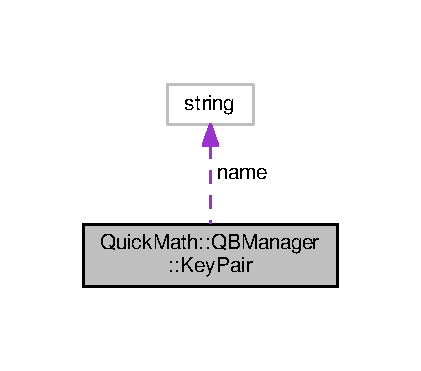
\includegraphics[width=202pt]{structQuickMath_1_1QBManager_1_1KeyPair__coll__graph}
\end{center}
\end{figure}
\subsection*{Public Member Functions}
\begin{DoxyCompactItemize}
\item 
\hyperlink{structQuickMath_1_1QBManager_1_1KeyPair_a1a0c2d088d2a4bc3eea9fc78a349db24}{Key\+Pair} ()=default
\item 
\hyperlink{structQuickMath_1_1QBManager_1_1KeyPair_a855867a1bc271998f22c91e683c49c79}{Key\+Pair} (std\+::string \hyperlink{structQuickMath_1_1QBManager_1_1KeyPair_a037ae369491b33991f062884f5f91c95}{name}, unsigned int \hyperlink{structQuickMath_1_1QBManager_1_1KeyPair_ab7f95fb28b5564fc80f6fa6923f22d5b}{idx})
\item 
bool \hyperlink{structQuickMath_1_1QBManager_1_1KeyPair_ab11227be6b4ff77384a916bedb7db6aa}{operator$<$} (const \hyperlink{structQuickMath_1_1QBManager_1_1KeyPair}{Key\+Pair} \&other) const 
\end{DoxyCompactItemize}
\subsection*{Public Attributes}
\begin{DoxyCompactItemize}
\item 
std\+::string \hyperlink{structQuickMath_1_1QBManager_1_1KeyPair_a037ae369491b33991f062884f5f91c95}{name}
\item 
int \hyperlink{structQuickMath_1_1QBManager_1_1KeyPair_ab7f95fb28b5564fc80f6fa6923f22d5b}{idx} = 0
\end{DoxyCompactItemize}


\subsection{Constructor \& Destructor Documentation}
\hypertarget{structQuickMath_1_1QBManager_1_1KeyPair_a1a0c2d088d2a4bc3eea9fc78a349db24}{}\index{Quick\+Math\+::\+Q\+B\+Manager\+::\+Key\+Pair@{Quick\+Math\+::\+Q\+B\+Manager\+::\+Key\+Pair}!Key\+Pair@{Key\+Pair}}
\index{Key\+Pair@{Key\+Pair}!Quick\+Math\+::\+Q\+B\+Manager\+::\+Key\+Pair@{Quick\+Math\+::\+Q\+B\+Manager\+::\+Key\+Pair}}
\subsubsection[{Key\+Pair}]{\setlength{\rightskip}{0pt plus 5cm}Quick\+Math\+::\+Q\+B\+Manager\+::\+Key\+Pair\+::\+Key\+Pair (
\begin{DoxyParamCaption}
{}
\end{DoxyParamCaption}
)\hspace{0.3cm}{\ttfamily [default]}}\label{structQuickMath_1_1QBManager_1_1KeyPair_a1a0c2d088d2a4bc3eea9fc78a349db24}
\hypertarget{structQuickMath_1_1QBManager_1_1KeyPair_a855867a1bc271998f22c91e683c49c79}{}\index{Quick\+Math\+::\+Q\+B\+Manager\+::\+Key\+Pair@{Quick\+Math\+::\+Q\+B\+Manager\+::\+Key\+Pair}!Key\+Pair@{Key\+Pair}}
\index{Key\+Pair@{Key\+Pair}!Quick\+Math\+::\+Q\+B\+Manager\+::\+Key\+Pair@{Quick\+Math\+::\+Q\+B\+Manager\+::\+Key\+Pair}}
\subsubsection[{Key\+Pair}]{\setlength{\rightskip}{0pt plus 5cm}Quick\+Math\+::\+Q\+B\+Manager\+::\+Key\+Pair\+::\+Key\+Pair (
\begin{DoxyParamCaption}
\item[{std\+::string}]{name, }
\item[{unsigned int}]{idx}
\end{DoxyParamCaption}
)\hspace{0.3cm}{\ttfamily [inline]}}\label{structQuickMath_1_1QBManager_1_1KeyPair_a855867a1bc271998f22c91e683c49c79}


\subsection{Member Function Documentation}
\hypertarget{structQuickMath_1_1QBManager_1_1KeyPair_ab11227be6b4ff77384a916bedb7db6aa}{}\index{Quick\+Math\+::\+Q\+B\+Manager\+::\+Key\+Pair@{Quick\+Math\+::\+Q\+B\+Manager\+::\+Key\+Pair}!operator$<$@{operator$<$}}
\index{operator$<$@{operator$<$}!Quick\+Math\+::\+Q\+B\+Manager\+::\+Key\+Pair@{Quick\+Math\+::\+Q\+B\+Manager\+::\+Key\+Pair}}
\subsubsection[{operator$<$}]{\setlength{\rightskip}{0pt plus 5cm}bool Quick\+Math\+::\+Q\+B\+Manager\+::\+Key\+Pair\+::operator$<$ (
\begin{DoxyParamCaption}
\item[{const {\bf Key\+Pair} \&}]{other}
\end{DoxyParamCaption}
) const\hspace{0.3cm}{\ttfamily [inline]}}\label{structQuickMath_1_1QBManager_1_1KeyPair_ab11227be6b4ff77384a916bedb7db6aa}


\subsection{Member Data Documentation}
\hypertarget{structQuickMath_1_1QBManager_1_1KeyPair_ab7f95fb28b5564fc80f6fa6923f22d5b}{}\index{Quick\+Math\+::\+Q\+B\+Manager\+::\+Key\+Pair@{Quick\+Math\+::\+Q\+B\+Manager\+::\+Key\+Pair}!idx@{idx}}
\index{idx@{idx}!Quick\+Math\+::\+Q\+B\+Manager\+::\+Key\+Pair@{Quick\+Math\+::\+Q\+B\+Manager\+::\+Key\+Pair}}
\subsubsection[{idx}]{\setlength{\rightskip}{0pt plus 5cm}int Quick\+Math\+::\+Q\+B\+Manager\+::\+Key\+Pair\+::idx = 0}\label{structQuickMath_1_1QBManager_1_1KeyPair_ab7f95fb28b5564fc80f6fa6923f22d5b}
\hypertarget{structQuickMath_1_1QBManager_1_1KeyPair_a037ae369491b33991f062884f5f91c95}{}\index{Quick\+Math\+::\+Q\+B\+Manager\+::\+Key\+Pair@{Quick\+Math\+::\+Q\+B\+Manager\+::\+Key\+Pair}!name@{name}}
\index{name@{name}!Quick\+Math\+::\+Q\+B\+Manager\+::\+Key\+Pair@{Quick\+Math\+::\+Q\+B\+Manager\+::\+Key\+Pair}}
\subsubsection[{name}]{\setlength{\rightskip}{0pt plus 5cm}std\+::string Quick\+Math\+::\+Q\+B\+Manager\+::\+Key\+Pair\+::name}\label{structQuickMath_1_1QBManager_1_1KeyPair_a037ae369491b33991f062884f5f91c95}


The documentation for this struct was generated from the following file\+:\begin{DoxyCompactItemize}
\item 
include/\+Q\+Bool/\hyperlink{QBManager_8h}{Q\+B\+Manager.\+h}\end{DoxyCompactItemize}

\hypertarget{classQuickMath_1_1QBAnd}{}\section{Quick\+Math\+:\+:Q\+B\+And Class Reference}
\label{classQuickMath_1_1QBAnd}\index{Quick\+Math\+::\+Q\+B\+And@{Quick\+Math\+::\+Q\+B\+And}}


{\ttfamily \#include $<$Q\+B\+And.\+h$>$}



Inheritance diagram for Quick\+Math\+:\+:Q\+B\+And\+:
\nopagebreak
\begin{figure}[H]
\begin{center}
\leavevmode
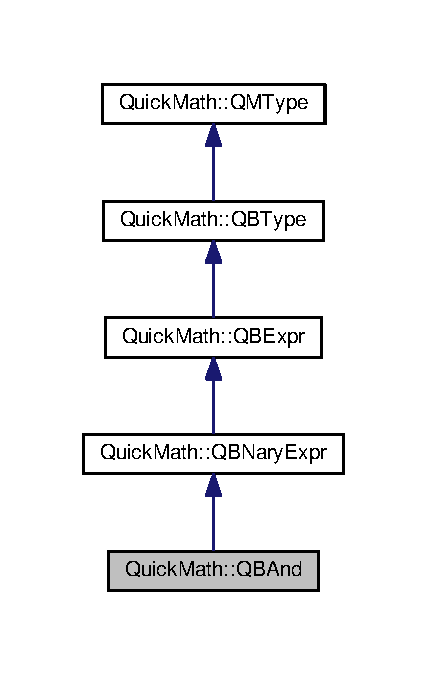
\includegraphics[width=205pt]{classQuickMath_1_1QBAnd__inherit__graph}
\end{center}
\end{figure}


Collaboration diagram for Quick\+Math\+:\+:Q\+B\+And\+:
\nopagebreak
\begin{figure}[H]
\begin{center}
\leavevmode
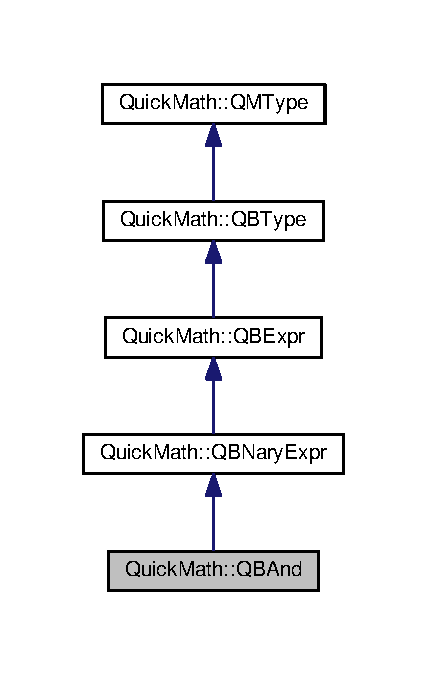
\includegraphics[width=205pt]{classQuickMath_1_1QBAnd__coll__graph}
\end{center}
\end{figure}
\subsection*{Public Member Functions}
\begin{DoxyCompactItemize}
\item 
\hyperlink{classQuickMath_1_1QBAnd_a77f6a049fa5aed5e5e0891ab786a302d}{Q\+B\+And} ()=default
\item 
\hyperlink{classQuickMath_1_1QBAnd_a826a9fd7bf5bb6b2a11f0b72efe48683}{Q\+B\+And} (const \hyperlink{classQuickMath_1_1QBType}{Q\+B\+Type} \&a, const \hyperlink{classQuickMath_1_1QBType}{Q\+B\+Type} \&b)
\item 
\hyperlink{classQuickMath_1_1QBAnd_ac40420b64b8eafda7d8f0f5098665d46}{Q\+B\+And} (std\+::unique\+\_\+ptr$<$ \hyperlink{classQuickMath_1_1QBType}{Q\+B\+Type} $>$ a, const \hyperlink{classQuickMath_1_1QBType}{Q\+B\+Type} \&b)
\item 
\hyperlink{classQuickMath_1_1QBAnd_a95861de48ff7878bb513037bd70f80d1}{Q\+B\+And} (const \hyperlink{classQuickMath_1_1QBType}{Q\+B\+Type} \&a, std\+::unique\+\_\+ptr$<$ \hyperlink{classQuickMath_1_1QBType}{Q\+B\+Type} $>$ b)
\item 
\hyperlink{classQuickMath_1_1QBAnd_a5e7578afa55e126db11feaf5139119a7}{Q\+B\+And} (std\+::unique\+\_\+ptr$<$ \hyperlink{classQuickMath_1_1QBType}{Q\+B\+Type} $>$ a, std\+::unique\+\_\+ptr$<$ \hyperlink{classQuickMath_1_1QBType}{Q\+B\+Type} $>$ b)
\item 
\hyperlink{classQuickMath_1_1QBAnd_a687345007975f87155350b33be4da198}{Q\+B\+And} (const \hyperlink{classQuickMath_1_1QBAnd}{Q\+B\+And} \&other)
\item 
std\+::string \hyperlink{classQuickMath_1_1QBAnd_abf6c063e663077fdddc4aae96bfbca27}{to\+String} () const 
\item 
\hyperlink{namespaceQuickMath_aec13b08c42d9f8e688241623c8b379a0}{Q\+B\+Value} \hyperlink{classQuickMath_1_1QBAnd_abd8953fcd0d25729cec8c7d78355d217}{value} () const 
\item 
std\+::unique\+\_\+ptr$<$ \hyperlink{classQuickMath_1_1QMType}{Q\+M\+Type} $>$ \hyperlink{classQuickMath_1_1QBAnd_a2a2957570e1b333c6190ecf1526c3124}{clone} () const 
\item 
bool \hyperlink{classQuickMath_1_1QBAnd_a9c722c8c7f3826faded75d70dd0f406c}{is\+And} () const 
\end{DoxyCompactItemize}
\subsection*{Additional Inherited Members}


\subsection{Constructor \& Destructor Documentation}
\hypertarget{classQuickMath_1_1QBAnd_a77f6a049fa5aed5e5e0891ab786a302d}{}\index{Quick\+Math\+::\+Q\+B\+And@{Quick\+Math\+::\+Q\+B\+And}!Q\+B\+And@{Q\+B\+And}}
\index{Q\+B\+And@{Q\+B\+And}!Quick\+Math\+::\+Q\+B\+And@{Quick\+Math\+::\+Q\+B\+And}}
\subsubsection[{Q\+B\+And}]{\setlength{\rightskip}{0pt plus 5cm}Quick\+Math\+::\+Q\+B\+And\+::\+Q\+B\+And (
\begin{DoxyParamCaption}
{}
\end{DoxyParamCaption}
)\hspace{0.3cm}{\ttfamily [default]}}\label{classQuickMath_1_1QBAnd_a77f6a049fa5aed5e5e0891ab786a302d}
\hypertarget{classQuickMath_1_1QBAnd_a826a9fd7bf5bb6b2a11f0b72efe48683}{}\index{Quick\+Math\+::\+Q\+B\+And@{Quick\+Math\+::\+Q\+B\+And}!Q\+B\+And@{Q\+B\+And}}
\index{Q\+B\+And@{Q\+B\+And}!Quick\+Math\+::\+Q\+B\+And@{Quick\+Math\+::\+Q\+B\+And}}
\subsubsection[{Q\+B\+And}]{\setlength{\rightskip}{0pt plus 5cm}Quick\+Math\+::\+Q\+B\+And\+::\+Q\+B\+And (
\begin{DoxyParamCaption}
\item[{const {\bf Q\+B\+Type} \&}]{a, }
\item[{const {\bf Q\+B\+Type} \&}]{b}
\end{DoxyParamCaption}
)}\label{classQuickMath_1_1QBAnd_a826a9fd7bf5bb6b2a11f0b72efe48683}
\hypertarget{classQuickMath_1_1QBAnd_ac40420b64b8eafda7d8f0f5098665d46}{}\index{Quick\+Math\+::\+Q\+B\+And@{Quick\+Math\+::\+Q\+B\+And}!Q\+B\+And@{Q\+B\+And}}
\index{Q\+B\+And@{Q\+B\+And}!Quick\+Math\+::\+Q\+B\+And@{Quick\+Math\+::\+Q\+B\+And}}
\subsubsection[{Q\+B\+And}]{\setlength{\rightskip}{0pt plus 5cm}Quick\+Math\+::\+Q\+B\+And\+::\+Q\+B\+And (
\begin{DoxyParamCaption}
\item[{std\+::unique\+\_\+ptr$<$ {\bf Q\+B\+Type} $>$}]{a, }
\item[{const {\bf Q\+B\+Type} \&}]{b}
\end{DoxyParamCaption}
)}\label{classQuickMath_1_1QBAnd_ac40420b64b8eafda7d8f0f5098665d46}
\hypertarget{classQuickMath_1_1QBAnd_a95861de48ff7878bb513037bd70f80d1}{}\index{Quick\+Math\+::\+Q\+B\+And@{Quick\+Math\+::\+Q\+B\+And}!Q\+B\+And@{Q\+B\+And}}
\index{Q\+B\+And@{Q\+B\+And}!Quick\+Math\+::\+Q\+B\+And@{Quick\+Math\+::\+Q\+B\+And}}
\subsubsection[{Q\+B\+And}]{\setlength{\rightskip}{0pt plus 5cm}Quick\+Math\+::\+Q\+B\+And\+::\+Q\+B\+And (
\begin{DoxyParamCaption}
\item[{const {\bf Q\+B\+Type} \&}]{a, }
\item[{std\+::unique\+\_\+ptr$<$ {\bf Q\+B\+Type} $>$}]{b}
\end{DoxyParamCaption}
)}\label{classQuickMath_1_1QBAnd_a95861de48ff7878bb513037bd70f80d1}
\hypertarget{classQuickMath_1_1QBAnd_a5e7578afa55e126db11feaf5139119a7}{}\index{Quick\+Math\+::\+Q\+B\+And@{Quick\+Math\+::\+Q\+B\+And}!Q\+B\+And@{Q\+B\+And}}
\index{Q\+B\+And@{Q\+B\+And}!Quick\+Math\+::\+Q\+B\+And@{Quick\+Math\+::\+Q\+B\+And}}
\subsubsection[{Q\+B\+And}]{\setlength{\rightskip}{0pt plus 5cm}Quick\+Math\+::\+Q\+B\+And\+::\+Q\+B\+And (
\begin{DoxyParamCaption}
\item[{std\+::unique\+\_\+ptr$<$ {\bf Q\+B\+Type} $>$}]{a, }
\item[{std\+::unique\+\_\+ptr$<$ {\bf Q\+B\+Type} $>$}]{b}
\end{DoxyParamCaption}
)}\label{classQuickMath_1_1QBAnd_a5e7578afa55e126db11feaf5139119a7}
\hypertarget{classQuickMath_1_1QBAnd_a687345007975f87155350b33be4da198}{}\index{Quick\+Math\+::\+Q\+B\+And@{Quick\+Math\+::\+Q\+B\+And}!Q\+B\+And@{Q\+B\+And}}
\index{Q\+B\+And@{Q\+B\+And}!Quick\+Math\+::\+Q\+B\+And@{Quick\+Math\+::\+Q\+B\+And}}
\subsubsection[{Q\+B\+And}]{\setlength{\rightskip}{0pt plus 5cm}Quick\+Math\+::\+Q\+B\+And\+::\+Q\+B\+And (
\begin{DoxyParamCaption}
\item[{const {\bf Q\+B\+And} \&}]{other}
\end{DoxyParamCaption}
)}\label{classQuickMath_1_1QBAnd_a687345007975f87155350b33be4da198}


\subsection{Member Function Documentation}
\hypertarget{classQuickMath_1_1QBAnd_a2a2957570e1b333c6190ecf1526c3124}{}\index{Quick\+Math\+::\+Q\+B\+And@{Quick\+Math\+::\+Q\+B\+And}!clone@{clone}}
\index{clone@{clone}!Quick\+Math\+::\+Q\+B\+And@{Quick\+Math\+::\+Q\+B\+And}}
\subsubsection[{clone}]{\setlength{\rightskip}{0pt plus 5cm}std\+::unique\+\_\+ptr$<$ {\bf Q\+M\+Type} $>$ Quick\+Math\+::\+Q\+B\+And\+::clone (
\begin{DoxyParamCaption}
{}
\end{DoxyParamCaption}
) const\hspace{0.3cm}{\ttfamily [virtual]}}\label{classQuickMath_1_1QBAnd_a2a2957570e1b333c6190ecf1526c3124}


Implements \hyperlink{classQuickMath_1_1QMType_a15b2a74a662417da99c6da9b7aaeff77}{Quick\+Math\+::\+Q\+M\+Type}.

\hypertarget{classQuickMath_1_1QBAnd_a9c722c8c7f3826faded75d70dd0f406c}{}\index{Quick\+Math\+::\+Q\+B\+And@{Quick\+Math\+::\+Q\+B\+And}!is\+And@{is\+And}}
\index{is\+And@{is\+And}!Quick\+Math\+::\+Q\+B\+And@{Quick\+Math\+::\+Q\+B\+And}}
\subsubsection[{is\+And}]{\setlength{\rightskip}{0pt plus 5cm}bool Quick\+Math\+::\+Q\+B\+And\+::is\+And (
\begin{DoxyParamCaption}
{}
\end{DoxyParamCaption}
) const\hspace{0.3cm}{\ttfamily [virtual]}}\label{classQuickMath_1_1QBAnd_a9c722c8c7f3826faded75d70dd0f406c}


Reimplemented from \hyperlink{classQuickMath_1_1QBType_a25cfa48db30dac38ace41b0997c089ab}{Quick\+Math\+::\+Q\+B\+Type}.

\hypertarget{classQuickMath_1_1QBAnd_abf6c063e663077fdddc4aae96bfbca27}{}\index{Quick\+Math\+::\+Q\+B\+And@{Quick\+Math\+::\+Q\+B\+And}!to\+String@{to\+String}}
\index{to\+String@{to\+String}!Quick\+Math\+::\+Q\+B\+And@{Quick\+Math\+::\+Q\+B\+And}}
\subsubsection[{to\+String}]{\setlength{\rightskip}{0pt plus 5cm}std\+::string Quick\+Math\+::\+Q\+B\+And\+::to\+String (
\begin{DoxyParamCaption}
{}
\end{DoxyParamCaption}
) const\hspace{0.3cm}{\ttfamily [virtual]}}\label{classQuickMath_1_1QBAnd_abf6c063e663077fdddc4aae96bfbca27}


Implements \hyperlink{classQuickMath_1_1QBType_a12a08061a73649a9f79995469f8297d2}{Quick\+Math\+::\+Q\+B\+Type}.

\hypertarget{classQuickMath_1_1QBAnd_abd8953fcd0d25729cec8c7d78355d217}{}\index{Quick\+Math\+::\+Q\+B\+And@{Quick\+Math\+::\+Q\+B\+And}!value@{value}}
\index{value@{value}!Quick\+Math\+::\+Q\+B\+And@{Quick\+Math\+::\+Q\+B\+And}}
\subsubsection[{value}]{\setlength{\rightskip}{0pt plus 5cm}{\bf Q\+B\+Value} Quick\+Math\+::\+Q\+B\+And\+::value (
\begin{DoxyParamCaption}
{}
\end{DoxyParamCaption}
) const\hspace{0.3cm}{\ttfamily [virtual]}}\label{classQuickMath_1_1QBAnd_abd8953fcd0d25729cec8c7d78355d217}


Implements \hyperlink{classQuickMath_1_1QBType_a3fa2589c7d1fa4a52e79193bef845eeb}{Quick\+Math\+::\+Q\+B\+Type}.



The documentation for this class was generated from the following files\+:\begin{DoxyCompactItemize}
\item 
include/\+Q\+Bool/\hyperlink{QBAnd_8h}{Q\+B\+And.\+h}\item 
src/\+Q\+Bool/\hyperlink{QBAnd_8cpp}{Q\+B\+And.\+cpp}\end{DoxyCompactItemize}

\hypertarget{classQuickMath_1_1QBBit}{}\section{Quick\+Math\+:\+:Q\+B\+Bit Class Reference}
\label{classQuickMath_1_1QBBit}\index{Quick\+Math\+::\+Q\+B\+Bit@{Quick\+Math\+::\+Q\+B\+Bit}}


{\ttfamily \#include $<$Q\+B\+Bit.\+h$>$}



Inheritance diagram for Quick\+Math\+:\+:Q\+B\+Bit\+:
\nopagebreak
\begin{figure}[H]
\begin{center}
\leavevmode
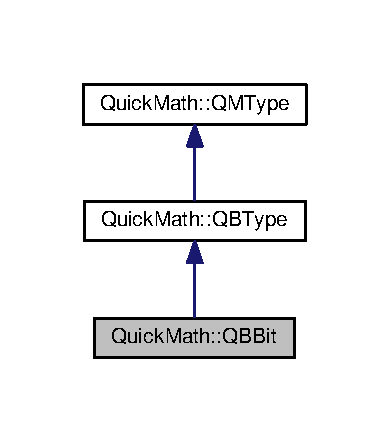
\includegraphics[width=187pt]{classQuickMath_1_1QBBit__inherit__graph}
\end{center}
\end{figure}


Collaboration diagram for Quick\+Math\+:\+:Q\+B\+Bit\+:
\nopagebreak
\begin{figure}[H]
\begin{center}
\leavevmode
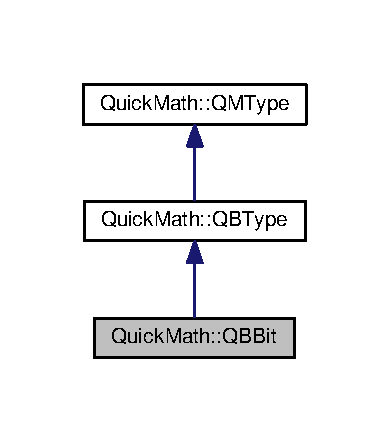
\includegraphics[width=187pt]{classQuickMath_1_1QBBit__coll__graph}
\end{center}
\end{figure}
\subsection*{Public Member Functions}
\begin{DoxyCompactItemize}
\item 
\hyperlink{classQuickMath_1_1QBBit_a5e11e1f0aa39500e8a9e6a2c69cddfa4}{Q\+B\+Bit} (std\+::shared\+\_\+ptr$<$ \hyperlink{classQuickMath_1_1QBBitShared}{Q\+B\+Bit\+Shared} $>$ \hyperlink{classQuickMath_1_1QBBit_ac2d748c7aa8ad849b2bdd5bc98d24caa}{bb})
\item 
void \hyperlink{classQuickMath_1_1QBBit_a4ec9d377770f994b72a3e23aee6a1314}{set\+Value} (\hyperlink{namespaceQuickMath_aec13b08c42d9f8e688241623c8b379a0}{Q\+B\+Value} val)
\item 
bool \hyperlink{classQuickMath_1_1QBBit_a6f570086177786f5bf8191505f9216c1}{is\+Var} () const 
\item 
std\+::string \hyperlink{classQuickMath_1_1QBBit_acf69bfd78922571f1f0ac146c4eed56f}{to\+String} () const 
\item 
\hyperlink{namespaceQuickMath_aec13b08c42d9f8e688241623c8b379a0}{Q\+B\+Value} \hyperlink{classQuickMath_1_1QBBit_add83657ec02a247eeb3883f8140d3223}{value} () const 
\item 
int64\+\_\+t \hyperlink{classQuickMath_1_1QBBit_a436915618ae2bc50324d5783b2d61f9c}{get\+Ref} () const 
\item 
std\+::unique\+\_\+ptr$<$ \hyperlink{classQuickMath_1_1QMType}{Q\+M\+Type} $>$ \hyperlink{classQuickMath_1_1QBBit_a5104a43946ee33625bc7b7ad02850d7a}{clone} () const 
\item 
unsigned int \hyperlink{classQuickMath_1_1QBBit_a14a19b5e9f00aa884eee8f54d111ec7a}{get\+Index} () const 
\item 
const std\+::string \& \hyperlink{classQuickMath_1_1QBBit_a7a314546144d02b0053374405d24d2b6}{get\+Name} () const 
\end{DoxyCompactItemize}
\subsection*{Private Attributes}
\begin{DoxyCompactItemize}
\item 
std\+::shared\+\_\+ptr$<$ \hyperlink{classQuickMath_1_1QBBitShared}{Q\+B\+Bit\+Shared} $>$ \hyperlink{classQuickMath_1_1QBBit_ac2d748c7aa8ad849b2bdd5bc98d24caa}{bb}
\end{DoxyCompactItemize}


\subsection{Constructor \& Destructor Documentation}
\hypertarget{classQuickMath_1_1QBBit_a5e11e1f0aa39500e8a9e6a2c69cddfa4}{}\index{Quick\+Math\+::\+Q\+B\+Bit@{Quick\+Math\+::\+Q\+B\+Bit}!Q\+B\+Bit@{Q\+B\+Bit}}
\index{Q\+B\+Bit@{Q\+B\+Bit}!Quick\+Math\+::\+Q\+B\+Bit@{Quick\+Math\+::\+Q\+B\+Bit}}
\subsubsection[{Q\+B\+Bit}]{\setlength{\rightskip}{0pt plus 5cm}Quick\+Math\+::\+Q\+B\+Bit\+::\+Q\+B\+Bit (
\begin{DoxyParamCaption}
\item[{std\+::shared\+\_\+ptr$<$ {\bf Q\+B\+Bit\+Shared} $>$}]{bb}
\end{DoxyParamCaption}
)}\label{classQuickMath_1_1QBBit_a5e11e1f0aa39500e8a9e6a2c69cddfa4}


\subsection{Member Function Documentation}
\hypertarget{classQuickMath_1_1QBBit_a5104a43946ee33625bc7b7ad02850d7a}{}\index{Quick\+Math\+::\+Q\+B\+Bit@{Quick\+Math\+::\+Q\+B\+Bit}!clone@{clone}}
\index{clone@{clone}!Quick\+Math\+::\+Q\+B\+Bit@{Quick\+Math\+::\+Q\+B\+Bit}}
\subsubsection[{clone}]{\setlength{\rightskip}{0pt plus 5cm}std\+::unique\+\_\+ptr$<$ {\bf Q\+M\+Type} $>$ Quick\+Math\+::\+Q\+B\+Bit\+::clone (
\begin{DoxyParamCaption}
{}
\end{DoxyParamCaption}
) const\hspace{0.3cm}{\ttfamily [virtual]}}\label{classQuickMath_1_1QBBit_a5104a43946ee33625bc7b7ad02850d7a}


Implements \hyperlink{classQuickMath_1_1QMType_a15b2a74a662417da99c6da9b7aaeff77}{Quick\+Math\+::\+Q\+M\+Type}.

\hypertarget{classQuickMath_1_1QBBit_a14a19b5e9f00aa884eee8f54d111ec7a}{}\index{Quick\+Math\+::\+Q\+B\+Bit@{Quick\+Math\+::\+Q\+B\+Bit}!get\+Index@{get\+Index}}
\index{get\+Index@{get\+Index}!Quick\+Math\+::\+Q\+B\+Bit@{Quick\+Math\+::\+Q\+B\+Bit}}
\subsubsection[{get\+Index}]{\setlength{\rightskip}{0pt plus 5cm}unsigned int Quick\+Math\+::\+Q\+B\+Bit\+::get\+Index (
\begin{DoxyParamCaption}
{}
\end{DoxyParamCaption}
) const}\label{classQuickMath_1_1QBBit_a14a19b5e9f00aa884eee8f54d111ec7a}
\hypertarget{classQuickMath_1_1QBBit_a7a314546144d02b0053374405d24d2b6}{}\index{Quick\+Math\+::\+Q\+B\+Bit@{Quick\+Math\+::\+Q\+B\+Bit}!get\+Name@{get\+Name}}
\index{get\+Name@{get\+Name}!Quick\+Math\+::\+Q\+B\+Bit@{Quick\+Math\+::\+Q\+B\+Bit}}
\subsubsection[{get\+Name}]{\setlength{\rightskip}{0pt plus 5cm}const std\+::string \& Quick\+Math\+::\+Q\+B\+Bit\+::get\+Name (
\begin{DoxyParamCaption}
{}
\end{DoxyParamCaption}
) const}\label{classQuickMath_1_1QBBit_a7a314546144d02b0053374405d24d2b6}
\hypertarget{classQuickMath_1_1QBBit_a436915618ae2bc50324d5783b2d61f9c}{}\index{Quick\+Math\+::\+Q\+B\+Bit@{Quick\+Math\+::\+Q\+B\+Bit}!get\+Ref@{get\+Ref}}
\index{get\+Ref@{get\+Ref}!Quick\+Math\+::\+Q\+B\+Bit@{Quick\+Math\+::\+Q\+B\+Bit}}
\subsubsection[{get\+Ref}]{\setlength{\rightskip}{0pt plus 5cm}int64\+\_\+t Quick\+Math\+::\+Q\+B\+Bit\+::get\+Ref (
\begin{DoxyParamCaption}
{}
\end{DoxyParamCaption}
) const}\label{classQuickMath_1_1QBBit_a436915618ae2bc50324d5783b2d61f9c}
\hypertarget{classQuickMath_1_1QBBit_a6f570086177786f5bf8191505f9216c1}{}\index{Quick\+Math\+::\+Q\+B\+Bit@{Quick\+Math\+::\+Q\+B\+Bit}!is\+Var@{is\+Var}}
\index{is\+Var@{is\+Var}!Quick\+Math\+::\+Q\+B\+Bit@{Quick\+Math\+::\+Q\+B\+Bit}}
\subsubsection[{is\+Var}]{\setlength{\rightskip}{0pt plus 5cm}bool Quick\+Math\+::\+Q\+B\+Bit\+::is\+Var (
\begin{DoxyParamCaption}
{}
\end{DoxyParamCaption}
) const\hspace{0.3cm}{\ttfamily [virtual]}}\label{classQuickMath_1_1QBBit_a6f570086177786f5bf8191505f9216c1}


Reimplemented from \hyperlink{classQuickMath_1_1QBType_a0f612bd5695bf0e1cc56ebb98b18cf18}{Quick\+Math\+::\+Q\+B\+Type}.

\hypertarget{classQuickMath_1_1QBBit_a4ec9d377770f994b72a3e23aee6a1314}{}\index{Quick\+Math\+::\+Q\+B\+Bit@{Quick\+Math\+::\+Q\+B\+Bit}!set\+Value@{set\+Value}}
\index{set\+Value@{set\+Value}!Quick\+Math\+::\+Q\+B\+Bit@{Quick\+Math\+::\+Q\+B\+Bit}}
\subsubsection[{set\+Value}]{\setlength{\rightskip}{0pt plus 5cm}void Quick\+Math\+::\+Q\+B\+Bit\+::set\+Value (
\begin{DoxyParamCaption}
\item[{{\bf Q\+B\+Value}}]{val}
\end{DoxyParamCaption}
)}\label{classQuickMath_1_1QBBit_a4ec9d377770f994b72a3e23aee6a1314}
\hypertarget{classQuickMath_1_1QBBit_acf69bfd78922571f1f0ac146c4eed56f}{}\index{Quick\+Math\+::\+Q\+B\+Bit@{Quick\+Math\+::\+Q\+B\+Bit}!to\+String@{to\+String}}
\index{to\+String@{to\+String}!Quick\+Math\+::\+Q\+B\+Bit@{Quick\+Math\+::\+Q\+B\+Bit}}
\subsubsection[{to\+String}]{\setlength{\rightskip}{0pt plus 5cm}std\+::string Quick\+Math\+::\+Q\+B\+Bit\+::to\+String (
\begin{DoxyParamCaption}
{}
\end{DoxyParamCaption}
) const\hspace{0.3cm}{\ttfamily [virtual]}}\label{classQuickMath_1_1QBBit_acf69bfd78922571f1f0ac146c4eed56f}


Implements \hyperlink{classQuickMath_1_1QBType_a12a08061a73649a9f79995469f8297d2}{Quick\+Math\+::\+Q\+B\+Type}.

\hypertarget{classQuickMath_1_1QBBit_add83657ec02a247eeb3883f8140d3223}{}\index{Quick\+Math\+::\+Q\+B\+Bit@{Quick\+Math\+::\+Q\+B\+Bit}!value@{value}}
\index{value@{value}!Quick\+Math\+::\+Q\+B\+Bit@{Quick\+Math\+::\+Q\+B\+Bit}}
\subsubsection[{value}]{\setlength{\rightskip}{0pt plus 5cm}{\bf Q\+B\+Value} Quick\+Math\+::\+Q\+B\+Bit\+::value (
\begin{DoxyParamCaption}
{}
\end{DoxyParamCaption}
) const\hspace{0.3cm}{\ttfamily [virtual]}}\label{classQuickMath_1_1QBBit_add83657ec02a247eeb3883f8140d3223}


Implements \hyperlink{classQuickMath_1_1QBType_a3fa2589c7d1fa4a52e79193bef845eeb}{Quick\+Math\+::\+Q\+B\+Type}.



\subsection{Member Data Documentation}
\hypertarget{classQuickMath_1_1QBBit_ac2d748c7aa8ad849b2bdd5bc98d24caa}{}\index{Quick\+Math\+::\+Q\+B\+Bit@{Quick\+Math\+::\+Q\+B\+Bit}!bb@{bb}}
\index{bb@{bb}!Quick\+Math\+::\+Q\+B\+Bit@{Quick\+Math\+::\+Q\+B\+Bit}}
\subsubsection[{bb}]{\setlength{\rightskip}{0pt plus 5cm}std\+::shared\+\_\+ptr$<${\bf Q\+B\+Bit\+Shared}$>$ Quick\+Math\+::\+Q\+B\+Bit\+::bb\hspace{0.3cm}{\ttfamily [private]}}\label{classQuickMath_1_1QBBit_ac2d748c7aa8ad849b2bdd5bc98d24caa}


The documentation for this class was generated from the following files\+:\begin{DoxyCompactItemize}
\item 
include/\+Q\+Bool/\hyperlink{QBBit_8h}{Q\+B\+Bit.\+h}\item 
src/\+Q\+Bool/\hyperlink{QBBit_8cpp}{Q\+B\+Bit.\+cpp}\end{DoxyCompactItemize}

\hypertarget{structQuickMath_1_1QBAlgo_1_1QBBitCmp}{}\section{Quick\+Math\+:\+:Q\+B\+Algo\+:\+:Q\+B\+Bit\+Cmp Struct Reference}
\label{structQuickMath_1_1QBAlgo_1_1QBBitCmp}\index{Quick\+Math\+::\+Q\+B\+Algo\+::\+Q\+B\+Bit\+Cmp@{Quick\+Math\+::\+Q\+B\+Algo\+::\+Q\+B\+Bit\+Cmp}}
\subsection*{Public Member Functions}
\begin{DoxyCompactItemize}
\item 
bool \hyperlink{structQuickMath_1_1QBAlgo_1_1QBBitCmp_afd6abeb29f6a01c51a2d31c214bbdb3a}{operator()} (const \hyperlink{classQuickMath_1_1QBBit}{Q\+B\+Bit} $\ast$a, const \hyperlink{classQuickMath_1_1QBBit}{Q\+B\+Bit} $\ast$b)
\end{DoxyCompactItemize}


\subsection{Member Function Documentation}
\hypertarget{structQuickMath_1_1QBAlgo_1_1QBBitCmp_afd6abeb29f6a01c51a2d31c214bbdb3a}{}\index{Quick\+Math\+::\+Q\+B\+Algo\+::\+Q\+B\+Bit\+Cmp@{Quick\+Math\+::\+Q\+B\+Algo\+::\+Q\+B\+Bit\+Cmp}!operator()@{operator()}}
\index{operator()@{operator()}!Quick\+Math\+::\+Q\+B\+Algo\+::\+Q\+B\+Bit\+Cmp@{Quick\+Math\+::\+Q\+B\+Algo\+::\+Q\+B\+Bit\+Cmp}}
\subsubsection[{operator()}]{\setlength{\rightskip}{0pt plus 5cm}bool Quick\+Math\+::\+Q\+B\+Algo\+::\+Q\+B\+Bit\+Cmp\+::operator() (
\begin{DoxyParamCaption}
\item[{const {\bf Q\+B\+Bit} $\ast$}]{a, }
\item[{const {\bf Q\+B\+Bit} $\ast$}]{b}
\end{DoxyParamCaption}
)\hspace{0.3cm}{\ttfamily [inline]}}\label{structQuickMath_1_1QBAlgo_1_1QBBitCmp_afd6abeb29f6a01c51a2d31c214bbdb3a}


The documentation for this struct was generated from the following file\+:\begin{DoxyCompactItemize}
\item 
src/\+Q\+Bool/\hyperlink{QBAlgorithms_8cpp}{Q\+B\+Algorithms.\+cpp}\end{DoxyCompactItemize}

\hypertarget{classQuickMath_1_1QBBitShared}{}\section{Quick\+Math\+:\+:Q\+B\+Bit\+Shared Class Reference}
\label{classQuickMath_1_1QBBitShared}\index{Quick\+Math\+::\+Q\+B\+Bit\+Shared@{Quick\+Math\+::\+Q\+B\+Bit\+Shared}}


{\ttfamily \#include $<$Q\+B\+Bit.\+h$>$}



Inheritance diagram for Quick\+Math\+:\+:Q\+B\+Bit\+Shared\+:
\nopagebreak
\begin{figure}[H]
\begin{center}
\leavevmode
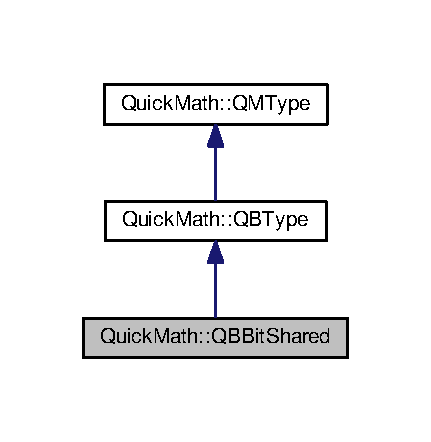
\includegraphics[width=207pt]{classQuickMath_1_1QBBitShared__inherit__graph}
\end{center}
\end{figure}


Collaboration diagram for Quick\+Math\+:\+:Q\+B\+Bit\+Shared\+:
\nopagebreak
\begin{figure}[H]
\begin{center}
\leavevmode
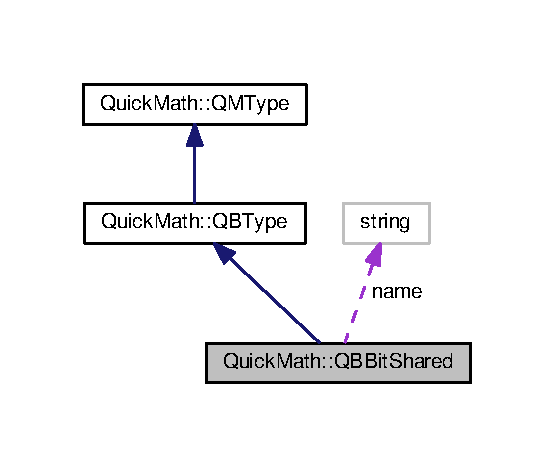
\includegraphics[width=266pt]{classQuickMath_1_1QBBitShared__coll__graph}
\end{center}
\end{figure}
\subsection*{Public Member Functions}
\begin{DoxyCompactItemize}
\item 
\hyperlink{classQuickMath_1_1QBBitShared_ad3a01433a2fe1d6689c61c0c0842d238}{Q\+B\+Bit\+Shared} (const std\+::string \&\hyperlink{classQuickMath_1_1QBBitShared_aa56ea4ce760dc0b941619974eb3ff626}{name}, unsigned int index=0, \hyperlink{namespaceQuickMath_aec13b08c42d9f8e688241623c8b379a0}{Q\+B\+Value} \hyperlink{classQuickMath_1_1QBBitShared_ae31aef3bff69da20dbc21799840c3b55}{val}=\hyperlink{namespaceQuickMath_aec13b08c42d9f8e688241623c8b379a0a88183b946cc5f0e8c96b2e66e1c74a7e}{Q\+B\+Value\+::\+Unknown})
\item 
\hyperlink{classQuickMath_1_1QBBitShared_ae6f5b0b474a37cd4ce4615d160713ac6}{Q\+B\+Bit\+Shared} (const \hyperlink{classQuickMath_1_1QBBitShared}{Q\+B\+Bit\+Shared} \&other)
\item 
virtual bool \hyperlink{classQuickMath_1_1QBBitShared_a69af2dec5fd73109c43f22c4230aa359}{is\+Var} () const 
\item 
virtual std\+::string \hyperlink{classQuickMath_1_1QBBitShared_ab1b3be4ae9548eac373e17038393f8a5}{to\+String} () const 
\item 
virtual \hyperlink{namespaceQuickMath_aec13b08c42d9f8e688241623c8b379a0}{Q\+B\+Value} \hyperlink{classQuickMath_1_1QBBitShared_a27cbff4bed10a2e1f0f958f07d2f3485}{value} () const 
\item 
unsigned int \hyperlink{classQuickMath_1_1QBBitShared_a98fb49161971cc3d78d2985fb94880b9}{get\+Index} () const 
\item 
int64\+\_\+t \hyperlink{classQuickMath_1_1QBBitShared_a158d2c15f27b1b5e2d25757a497bf178}{get\+Ref} () const 
\item 
const std\+::string \& \hyperlink{classQuickMath_1_1QBBitShared_adb5a57410ff5faf4add199a8ca7153be}{get\+Name} () const 
\item 
void \hyperlink{classQuickMath_1_1QBBitShared_a97bc55fd78add03023d69806b4df7723}{set\+Var} (\hyperlink{namespaceQuickMath_aec13b08c42d9f8e688241623c8b379a0}{Q\+B\+Value} \hyperlink{classQuickMath_1_1QBBitShared_ae31aef3bff69da20dbc21799840c3b55}{val})
\item 
std\+::unique\+\_\+ptr$<$ \hyperlink{classQuickMath_1_1QMType}{Q\+M\+Type} $>$ \hyperlink{classQuickMath_1_1QBBitShared_a8664352f6b5fa48070ffc4fa237a394e}{clone} () const 
\end{DoxyCompactItemize}
\subsection*{Private Attributes}
\begin{DoxyCompactItemize}
\item 
\hyperlink{namespaceQuickMath_aec13b08c42d9f8e688241623c8b379a0}{Q\+B\+Value} \hyperlink{classQuickMath_1_1QBBitShared_ae31aef3bff69da20dbc21799840c3b55}{val} = \hyperlink{namespaceQuickMath_aec13b08c42d9f8e688241623c8b379a0a88183b946cc5f0e8c96b2e66e1c74a7e}{Q\+B\+Value\+::\+Unknown}
\item 
unsigned int \hyperlink{classQuickMath_1_1QBBitShared_aa59b2fc1ed73d6170a9a26a5b7aa866c}{idx} = 0
\item 
int64\+\_\+t \hyperlink{classQuickMath_1_1QBBitShared_a0b5f238b3b0c959e54c5aeb9a6d4958b}{ref} = 0
\item 
std\+::string \hyperlink{classQuickMath_1_1QBBitShared_aa56ea4ce760dc0b941619974eb3ff626}{name} = \char`\"{}\char`\"{}
\end{DoxyCompactItemize}
\subsection*{Static Private Attributes}
\begin{DoxyCompactItemize}
\item 
static int64\+\_\+t \hyperlink{classQuickMath_1_1QBBitShared_a049ce447fd2651cf1985874e03a76430}{ref\+Cnt} = 0
\end{DoxyCompactItemize}


\subsection{Constructor \& Destructor Documentation}
\hypertarget{classQuickMath_1_1QBBitShared_ad3a01433a2fe1d6689c61c0c0842d238}{}\index{Quick\+Math\+::\+Q\+B\+Bit\+Shared@{Quick\+Math\+::\+Q\+B\+Bit\+Shared}!Q\+B\+Bit\+Shared@{Q\+B\+Bit\+Shared}}
\index{Q\+B\+Bit\+Shared@{Q\+B\+Bit\+Shared}!Quick\+Math\+::\+Q\+B\+Bit\+Shared@{Quick\+Math\+::\+Q\+B\+Bit\+Shared}}
\subsubsection[{Q\+B\+Bit\+Shared}]{\setlength{\rightskip}{0pt plus 5cm}Quick\+Math\+::\+Q\+B\+Bit\+Shared\+::\+Q\+B\+Bit\+Shared (
\begin{DoxyParamCaption}
\item[{const std\+::string \&}]{name, }
\item[{unsigned int}]{index = {\ttfamily 0}, }
\item[{{\bf Q\+B\+Value}}]{val = {\ttfamily {\bf Q\+B\+Value\+::\+Unknown}}}
\end{DoxyParamCaption}
)}\label{classQuickMath_1_1QBBitShared_ad3a01433a2fe1d6689c61c0c0842d238}
\hypertarget{classQuickMath_1_1QBBitShared_ae6f5b0b474a37cd4ce4615d160713ac6}{}\index{Quick\+Math\+::\+Q\+B\+Bit\+Shared@{Quick\+Math\+::\+Q\+B\+Bit\+Shared}!Q\+B\+Bit\+Shared@{Q\+B\+Bit\+Shared}}
\index{Q\+B\+Bit\+Shared@{Q\+B\+Bit\+Shared}!Quick\+Math\+::\+Q\+B\+Bit\+Shared@{Quick\+Math\+::\+Q\+B\+Bit\+Shared}}
\subsubsection[{Q\+B\+Bit\+Shared}]{\setlength{\rightskip}{0pt plus 5cm}Quick\+Math\+::\+Q\+B\+Bit\+Shared\+::\+Q\+B\+Bit\+Shared (
\begin{DoxyParamCaption}
\item[{const {\bf Q\+B\+Bit\+Shared} \&}]{other}
\end{DoxyParamCaption}
)}\label{classQuickMath_1_1QBBitShared_ae6f5b0b474a37cd4ce4615d160713ac6}


\subsection{Member Function Documentation}
\hypertarget{classQuickMath_1_1QBBitShared_a8664352f6b5fa48070ffc4fa237a394e}{}\index{Quick\+Math\+::\+Q\+B\+Bit\+Shared@{Quick\+Math\+::\+Q\+B\+Bit\+Shared}!clone@{clone}}
\index{clone@{clone}!Quick\+Math\+::\+Q\+B\+Bit\+Shared@{Quick\+Math\+::\+Q\+B\+Bit\+Shared}}
\subsubsection[{clone}]{\setlength{\rightskip}{0pt plus 5cm}std\+::unique\+\_\+ptr$<$ {\bf Q\+M\+Type} $>$ Quick\+Math\+::\+Q\+B\+Bit\+Shared\+::clone (
\begin{DoxyParamCaption}
{}
\end{DoxyParamCaption}
) const\hspace{0.3cm}{\ttfamily [virtual]}}\label{classQuickMath_1_1QBBitShared_a8664352f6b5fa48070ffc4fa237a394e}


Implements \hyperlink{classQuickMath_1_1QMType_a15b2a74a662417da99c6da9b7aaeff77}{Quick\+Math\+::\+Q\+M\+Type}.

\hypertarget{classQuickMath_1_1QBBitShared_a98fb49161971cc3d78d2985fb94880b9}{}\index{Quick\+Math\+::\+Q\+B\+Bit\+Shared@{Quick\+Math\+::\+Q\+B\+Bit\+Shared}!get\+Index@{get\+Index}}
\index{get\+Index@{get\+Index}!Quick\+Math\+::\+Q\+B\+Bit\+Shared@{Quick\+Math\+::\+Q\+B\+Bit\+Shared}}
\subsubsection[{get\+Index}]{\setlength{\rightskip}{0pt plus 5cm}unsigned int Quick\+Math\+::\+Q\+B\+Bit\+Shared\+::get\+Index (
\begin{DoxyParamCaption}
{}
\end{DoxyParamCaption}
) const}\label{classQuickMath_1_1QBBitShared_a98fb49161971cc3d78d2985fb94880b9}
\hypertarget{classQuickMath_1_1QBBitShared_adb5a57410ff5faf4add199a8ca7153be}{}\index{Quick\+Math\+::\+Q\+B\+Bit\+Shared@{Quick\+Math\+::\+Q\+B\+Bit\+Shared}!get\+Name@{get\+Name}}
\index{get\+Name@{get\+Name}!Quick\+Math\+::\+Q\+B\+Bit\+Shared@{Quick\+Math\+::\+Q\+B\+Bit\+Shared}}
\subsubsection[{get\+Name}]{\setlength{\rightskip}{0pt plus 5cm}const std\+::string \& Quick\+Math\+::\+Q\+B\+Bit\+Shared\+::get\+Name (
\begin{DoxyParamCaption}
{}
\end{DoxyParamCaption}
) const}\label{classQuickMath_1_1QBBitShared_adb5a57410ff5faf4add199a8ca7153be}
\hypertarget{classQuickMath_1_1QBBitShared_a158d2c15f27b1b5e2d25757a497bf178}{}\index{Quick\+Math\+::\+Q\+B\+Bit\+Shared@{Quick\+Math\+::\+Q\+B\+Bit\+Shared}!get\+Ref@{get\+Ref}}
\index{get\+Ref@{get\+Ref}!Quick\+Math\+::\+Q\+B\+Bit\+Shared@{Quick\+Math\+::\+Q\+B\+Bit\+Shared}}
\subsubsection[{get\+Ref}]{\setlength{\rightskip}{0pt plus 5cm}int64\+\_\+t Quick\+Math\+::\+Q\+B\+Bit\+Shared\+::get\+Ref (
\begin{DoxyParamCaption}
{}
\end{DoxyParamCaption}
) const}\label{classQuickMath_1_1QBBitShared_a158d2c15f27b1b5e2d25757a497bf178}
\hypertarget{classQuickMath_1_1QBBitShared_a69af2dec5fd73109c43f22c4230aa359}{}\index{Quick\+Math\+::\+Q\+B\+Bit\+Shared@{Quick\+Math\+::\+Q\+B\+Bit\+Shared}!is\+Var@{is\+Var}}
\index{is\+Var@{is\+Var}!Quick\+Math\+::\+Q\+B\+Bit\+Shared@{Quick\+Math\+::\+Q\+B\+Bit\+Shared}}
\subsubsection[{is\+Var}]{\setlength{\rightskip}{0pt plus 5cm}bool Quick\+Math\+::\+Q\+B\+Bit\+Shared\+::is\+Var (
\begin{DoxyParamCaption}
{}
\end{DoxyParamCaption}
) const\hspace{0.3cm}{\ttfamily [virtual]}}\label{classQuickMath_1_1QBBitShared_a69af2dec5fd73109c43f22c4230aa359}


Reimplemented from \hyperlink{classQuickMath_1_1QBType_a0f612bd5695bf0e1cc56ebb98b18cf18}{Quick\+Math\+::\+Q\+B\+Type}.

\hypertarget{classQuickMath_1_1QBBitShared_a97bc55fd78add03023d69806b4df7723}{}\index{Quick\+Math\+::\+Q\+B\+Bit\+Shared@{Quick\+Math\+::\+Q\+B\+Bit\+Shared}!set\+Var@{set\+Var}}
\index{set\+Var@{set\+Var}!Quick\+Math\+::\+Q\+B\+Bit\+Shared@{Quick\+Math\+::\+Q\+B\+Bit\+Shared}}
\subsubsection[{set\+Var}]{\setlength{\rightskip}{0pt plus 5cm}void Quick\+Math\+::\+Q\+B\+Bit\+Shared\+::set\+Var (
\begin{DoxyParamCaption}
\item[{{\bf Q\+B\+Value}}]{val}
\end{DoxyParamCaption}
)}\label{classQuickMath_1_1QBBitShared_a97bc55fd78add03023d69806b4df7723}
\hypertarget{classQuickMath_1_1QBBitShared_ab1b3be4ae9548eac373e17038393f8a5}{}\index{Quick\+Math\+::\+Q\+B\+Bit\+Shared@{Quick\+Math\+::\+Q\+B\+Bit\+Shared}!to\+String@{to\+String}}
\index{to\+String@{to\+String}!Quick\+Math\+::\+Q\+B\+Bit\+Shared@{Quick\+Math\+::\+Q\+B\+Bit\+Shared}}
\subsubsection[{to\+String}]{\setlength{\rightskip}{0pt plus 5cm}std\+::string Quick\+Math\+::\+Q\+B\+Bit\+Shared\+::to\+String (
\begin{DoxyParamCaption}
{}
\end{DoxyParamCaption}
) const\hspace{0.3cm}{\ttfamily [virtual]}}\label{classQuickMath_1_1QBBitShared_ab1b3be4ae9548eac373e17038393f8a5}


Implements \hyperlink{classQuickMath_1_1QBType_a12a08061a73649a9f79995469f8297d2}{Quick\+Math\+::\+Q\+B\+Type}.

\hypertarget{classQuickMath_1_1QBBitShared_a27cbff4bed10a2e1f0f958f07d2f3485}{}\index{Quick\+Math\+::\+Q\+B\+Bit\+Shared@{Quick\+Math\+::\+Q\+B\+Bit\+Shared}!value@{value}}
\index{value@{value}!Quick\+Math\+::\+Q\+B\+Bit\+Shared@{Quick\+Math\+::\+Q\+B\+Bit\+Shared}}
\subsubsection[{value}]{\setlength{\rightskip}{0pt plus 5cm}{\bf Q\+B\+Value} Quick\+Math\+::\+Q\+B\+Bit\+Shared\+::value (
\begin{DoxyParamCaption}
{}
\end{DoxyParamCaption}
) const\hspace{0.3cm}{\ttfamily [virtual]}}\label{classQuickMath_1_1QBBitShared_a27cbff4bed10a2e1f0f958f07d2f3485}


Implements \hyperlink{classQuickMath_1_1QBType_a3fa2589c7d1fa4a52e79193bef845eeb}{Quick\+Math\+::\+Q\+B\+Type}.



\subsection{Member Data Documentation}
\hypertarget{classQuickMath_1_1QBBitShared_aa59b2fc1ed73d6170a9a26a5b7aa866c}{}\index{Quick\+Math\+::\+Q\+B\+Bit\+Shared@{Quick\+Math\+::\+Q\+B\+Bit\+Shared}!idx@{idx}}
\index{idx@{idx}!Quick\+Math\+::\+Q\+B\+Bit\+Shared@{Quick\+Math\+::\+Q\+B\+Bit\+Shared}}
\subsubsection[{idx}]{\setlength{\rightskip}{0pt plus 5cm}unsigned int Quick\+Math\+::\+Q\+B\+Bit\+Shared\+::idx = 0\hspace{0.3cm}{\ttfamily [private]}}\label{classQuickMath_1_1QBBitShared_aa59b2fc1ed73d6170a9a26a5b7aa866c}
\hypertarget{classQuickMath_1_1QBBitShared_aa56ea4ce760dc0b941619974eb3ff626}{}\index{Quick\+Math\+::\+Q\+B\+Bit\+Shared@{Quick\+Math\+::\+Q\+B\+Bit\+Shared}!name@{name}}
\index{name@{name}!Quick\+Math\+::\+Q\+B\+Bit\+Shared@{Quick\+Math\+::\+Q\+B\+Bit\+Shared}}
\subsubsection[{name}]{\setlength{\rightskip}{0pt plus 5cm}std\+::string Quick\+Math\+::\+Q\+B\+Bit\+Shared\+::name = \char`\"{}\char`\"{}\hspace{0.3cm}{\ttfamily [private]}}\label{classQuickMath_1_1QBBitShared_aa56ea4ce760dc0b941619974eb3ff626}
\hypertarget{classQuickMath_1_1QBBitShared_a0b5f238b3b0c959e54c5aeb9a6d4958b}{}\index{Quick\+Math\+::\+Q\+B\+Bit\+Shared@{Quick\+Math\+::\+Q\+B\+Bit\+Shared}!ref@{ref}}
\index{ref@{ref}!Quick\+Math\+::\+Q\+B\+Bit\+Shared@{Quick\+Math\+::\+Q\+B\+Bit\+Shared}}
\subsubsection[{ref}]{\setlength{\rightskip}{0pt plus 5cm}int64\+\_\+t Quick\+Math\+::\+Q\+B\+Bit\+Shared\+::ref = 0\hspace{0.3cm}{\ttfamily [private]}}\label{classQuickMath_1_1QBBitShared_a0b5f238b3b0c959e54c5aeb9a6d4958b}
\hypertarget{classQuickMath_1_1QBBitShared_a049ce447fd2651cf1985874e03a76430}{}\index{Quick\+Math\+::\+Q\+B\+Bit\+Shared@{Quick\+Math\+::\+Q\+B\+Bit\+Shared}!ref\+Cnt@{ref\+Cnt}}
\index{ref\+Cnt@{ref\+Cnt}!Quick\+Math\+::\+Q\+B\+Bit\+Shared@{Quick\+Math\+::\+Q\+B\+Bit\+Shared}}
\subsubsection[{ref\+Cnt}]{\setlength{\rightskip}{0pt plus 5cm}int64\+\_\+t Quick\+Math\+::\+Q\+B\+Bit\+Shared\+::ref\+Cnt = 0\hspace{0.3cm}{\ttfamily [static]}, {\ttfamily [private]}}\label{classQuickMath_1_1QBBitShared_a049ce447fd2651cf1985874e03a76430}
\hypertarget{classQuickMath_1_1QBBitShared_ae31aef3bff69da20dbc21799840c3b55}{}\index{Quick\+Math\+::\+Q\+B\+Bit\+Shared@{Quick\+Math\+::\+Q\+B\+Bit\+Shared}!val@{val}}
\index{val@{val}!Quick\+Math\+::\+Q\+B\+Bit\+Shared@{Quick\+Math\+::\+Q\+B\+Bit\+Shared}}
\subsubsection[{val}]{\setlength{\rightskip}{0pt plus 5cm}{\bf Q\+B\+Value} Quick\+Math\+::\+Q\+B\+Bit\+Shared\+::val = {\bf Q\+B\+Value\+::\+Unknown}\hspace{0.3cm}{\ttfamily [private]}}\label{classQuickMath_1_1QBBitShared_ae31aef3bff69da20dbc21799840c3b55}


The documentation for this class was generated from the following files\+:\begin{DoxyCompactItemize}
\item 
include/\+Q\+Bool/\hyperlink{QBBit_8h}{Q\+B\+Bit.\+h}\item 
src/\+Q\+Bool/\hyperlink{QBBit_8cpp}{Q\+B\+Bit.\+cpp}\end{DoxyCompactItemize}

\hypertarget{classQuickMath_1_1QBConstant}{}\section{Quick\+Math\+:\+:Q\+B\+Constant Class Reference}
\label{classQuickMath_1_1QBConstant}\index{Quick\+Math\+::\+Q\+B\+Constant@{Quick\+Math\+::\+Q\+B\+Constant}}


{\ttfamily \#include $<$Q\+B\+Constants.\+h$>$}



Inheritance diagram for Quick\+Math\+:\+:Q\+B\+Constant\+:
\nopagebreak
\begin{figure}[H]
\begin{center}
\leavevmode
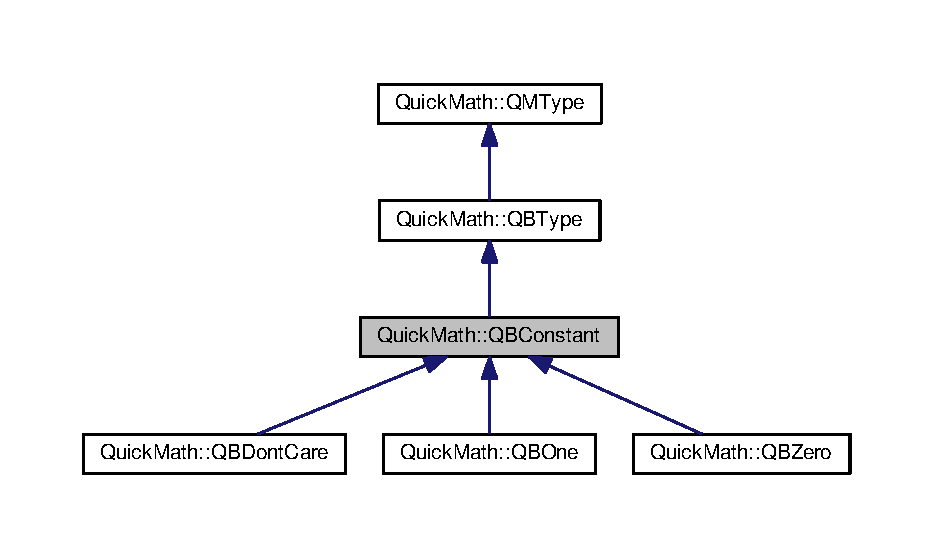
\includegraphics[width=350pt]{classQuickMath_1_1QBConstant__inherit__graph}
\end{center}
\end{figure}


Collaboration diagram for Quick\+Math\+:\+:Q\+B\+Constant\+:
\nopagebreak
\begin{figure}[H]
\begin{center}
\leavevmode
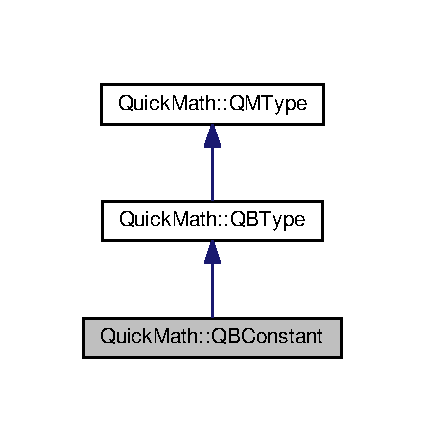
\includegraphics[width=204pt]{classQuickMath_1_1QBConstant__coll__graph}
\end{center}
\end{figure}
\subsection*{Public Member Functions}
\begin{DoxyCompactItemize}
\item 
bool \hyperlink{classQuickMath_1_1QBConstant_ac9ca2e6c87214135a275364956c66bae}{is\+Var} () const 
\item 
bool \hyperlink{classQuickMath_1_1QBConstant_a6e7ee651a6a0436a16575064f401a941}{is\+Expr} () const 
\item 
virtual std\+::string \hyperlink{classQuickMath_1_1QBConstant_a4e277add258b38b9f43da6dde48cd468}{to\+String} () const 
\item 
virtual \hyperlink{namespaceQuickMath_aec13b08c42d9f8e688241623c8b379a0}{Q\+B\+Value} \hyperlink{classQuickMath_1_1QBConstant_a399a700088d6327765b88652cea43c0e}{value} () const =0
\item 
bool \hyperlink{classQuickMath_1_1QBConstant_a750e108df9ba76a91a2e1096f01c5113}{is\+And} () const 
\item 
virtual bool \hyperlink{classQuickMath_1_1QBConstant_ad9da48094fec1db5dbba35d362d56bf6}{is\+Or} () const 
\item 
virtual bool \hyperlink{classQuickMath_1_1QBConstant_ae940dddd20874cec5c10b3fe6faf8bb2}{is\+Not} () const 
\end{DoxyCompactItemize}


\subsection{Member Function Documentation}
\hypertarget{classQuickMath_1_1QBConstant_a750e108df9ba76a91a2e1096f01c5113}{}\index{Quick\+Math\+::\+Q\+B\+Constant@{Quick\+Math\+::\+Q\+B\+Constant}!is\+And@{is\+And}}
\index{is\+And@{is\+And}!Quick\+Math\+::\+Q\+B\+Constant@{Quick\+Math\+::\+Q\+B\+Constant}}
\subsubsection[{is\+And}]{\setlength{\rightskip}{0pt plus 5cm}bool Quick\+Math\+::\+Q\+B\+Constant\+::is\+And (
\begin{DoxyParamCaption}
{}
\end{DoxyParamCaption}
) const\hspace{0.3cm}{\ttfamily [inline]}, {\ttfamily [virtual]}}\label{classQuickMath_1_1QBConstant_a750e108df9ba76a91a2e1096f01c5113}


Reimplemented from \hyperlink{classQuickMath_1_1QBType_a25cfa48db30dac38ace41b0997c089ab}{Quick\+Math\+::\+Q\+B\+Type}.

\hypertarget{classQuickMath_1_1QBConstant_a6e7ee651a6a0436a16575064f401a941}{}\index{Quick\+Math\+::\+Q\+B\+Constant@{Quick\+Math\+::\+Q\+B\+Constant}!is\+Expr@{is\+Expr}}
\index{is\+Expr@{is\+Expr}!Quick\+Math\+::\+Q\+B\+Constant@{Quick\+Math\+::\+Q\+B\+Constant}}
\subsubsection[{is\+Expr}]{\setlength{\rightskip}{0pt plus 5cm}bool Quick\+Math\+::\+Q\+B\+Constant\+::is\+Expr (
\begin{DoxyParamCaption}
{}
\end{DoxyParamCaption}
) const\hspace{0.3cm}{\ttfamily [virtual]}}\label{classQuickMath_1_1QBConstant_a6e7ee651a6a0436a16575064f401a941}


Reimplemented from \hyperlink{classQuickMath_1_1QBType_a773a28a659747ec2a5c13d2a6f401404}{Quick\+Math\+::\+Q\+B\+Type}.

\hypertarget{classQuickMath_1_1QBConstant_ae940dddd20874cec5c10b3fe6faf8bb2}{}\index{Quick\+Math\+::\+Q\+B\+Constant@{Quick\+Math\+::\+Q\+B\+Constant}!is\+Not@{is\+Not}}
\index{is\+Not@{is\+Not}!Quick\+Math\+::\+Q\+B\+Constant@{Quick\+Math\+::\+Q\+B\+Constant}}
\subsubsection[{is\+Not}]{\setlength{\rightskip}{0pt plus 5cm}virtual bool Quick\+Math\+::\+Q\+B\+Constant\+::is\+Not (
\begin{DoxyParamCaption}
{}
\end{DoxyParamCaption}
) const\hspace{0.3cm}{\ttfamily [inline]}, {\ttfamily [virtual]}}\label{classQuickMath_1_1QBConstant_ae940dddd20874cec5c10b3fe6faf8bb2}


Reimplemented from \hyperlink{classQuickMath_1_1QBType_a34cdcf8324b2091eae169992c1fcfa5b}{Quick\+Math\+::\+Q\+B\+Type}.

\hypertarget{classQuickMath_1_1QBConstant_ad9da48094fec1db5dbba35d362d56bf6}{}\index{Quick\+Math\+::\+Q\+B\+Constant@{Quick\+Math\+::\+Q\+B\+Constant}!is\+Or@{is\+Or}}
\index{is\+Or@{is\+Or}!Quick\+Math\+::\+Q\+B\+Constant@{Quick\+Math\+::\+Q\+B\+Constant}}
\subsubsection[{is\+Or}]{\setlength{\rightskip}{0pt plus 5cm}virtual bool Quick\+Math\+::\+Q\+B\+Constant\+::is\+Or (
\begin{DoxyParamCaption}
{}
\end{DoxyParamCaption}
) const\hspace{0.3cm}{\ttfamily [inline]}, {\ttfamily [virtual]}}\label{classQuickMath_1_1QBConstant_ad9da48094fec1db5dbba35d362d56bf6}


Reimplemented from \hyperlink{classQuickMath_1_1QBType_a7c76be740f838beb84ea0b6b7c8cfeda}{Quick\+Math\+::\+Q\+B\+Type}.

\hypertarget{classQuickMath_1_1QBConstant_ac9ca2e6c87214135a275364956c66bae}{}\index{Quick\+Math\+::\+Q\+B\+Constant@{Quick\+Math\+::\+Q\+B\+Constant}!is\+Var@{is\+Var}}
\index{is\+Var@{is\+Var}!Quick\+Math\+::\+Q\+B\+Constant@{Quick\+Math\+::\+Q\+B\+Constant}}
\subsubsection[{is\+Var}]{\setlength{\rightskip}{0pt plus 5cm}bool Quick\+Math\+::\+Q\+B\+Constant\+::is\+Var (
\begin{DoxyParamCaption}
{}
\end{DoxyParamCaption}
) const\hspace{0.3cm}{\ttfamily [virtual]}}\label{classQuickMath_1_1QBConstant_ac9ca2e6c87214135a275364956c66bae}


Reimplemented from \hyperlink{classQuickMath_1_1QBType_a0f612bd5695bf0e1cc56ebb98b18cf18}{Quick\+Math\+::\+Q\+B\+Type}.

\hypertarget{classQuickMath_1_1QBConstant_a4e277add258b38b9f43da6dde48cd468}{}\index{Quick\+Math\+::\+Q\+B\+Constant@{Quick\+Math\+::\+Q\+B\+Constant}!to\+String@{to\+String}}
\index{to\+String@{to\+String}!Quick\+Math\+::\+Q\+B\+Constant@{Quick\+Math\+::\+Q\+B\+Constant}}
\subsubsection[{to\+String}]{\setlength{\rightskip}{0pt plus 5cm}std\+::string Quick\+Math\+::\+Q\+B\+Constant\+::to\+String (
\begin{DoxyParamCaption}
{}
\end{DoxyParamCaption}
) const\hspace{0.3cm}{\ttfamily [virtual]}}\label{classQuickMath_1_1QBConstant_a4e277add258b38b9f43da6dde48cd468}


Implements \hyperlink{classQuickMath_1_1QBType_a12a08061a73649a9f79995469f8297d2}{Quick\+Math\+::\+Q\+B\+Type}.

\hypertarget{classQuickMath_1_1QBConstant_a399a700088d6327765b88652cea43c0e}{}\index{Quick\+Math\+::\+Q\+B\+Constant@{Quick\+Math\+::\+Q\+B\+Constant}!value@{value}}
\index{value@{value}!Quick\+Math\+::\+Q\+B\+Constant@{Quick\+Math\+::\+Q\+B\+Constant}}
\subsubsection[{value}]{\setlength{\rightskip}{0pt plus 5cm}virtual {\bf Q\+B\+Value} Quick\+Math\+::\+Q\+B\+Constant\+::value (
\begin{DoxyParamCaption}
{}
\end{DoxyParamCaption}
) const\hspace{0.3cm}{\ttfamily [pure virtual]}}\label{classQuickMath_1_1QBConstant_a399a700088d6327765b88652cea43c0e}


Implements \hyperlink{classQuickMath_1_1QBType_a3fa2589c7d1fa4a52e79193bef845eeb}{Quick\+Math\+::\+Q\+B\+Type}.



Implemented in \hyperlink{classQuickMath_1_1QBDontCare_a40a7cfa35c7e91d392493277d3e5078e}{Quick\+Math\+::\+Q\+B\+Dont\+Care}, \hyperlink{classQuickMath_1_1QBZero_a1e7a0a5ca21ee665eccfc59ac7702403}{Quick\+Math\+::\+Q\+B\+Zero}, and \hyperlink{classQuickMath_1_1QBOne_a2cc8ebd48be0d6edbfe0356d54d14919}{Quick\+Math\+::\+Q\+B\+One}.



The documentation for this class was generated from the following files\+:\begin{DoxyCompactItemize}
\item 
include/\+Q\+Bool/\hyperlink{QBConstants_8h}{Q\+B\+Constants.\+h}\item 
src/\+Q\+Bool/\hyperlink{QBConstants_8cpp}{Q\+B\+Constants.\+cpp}\end{DoxyCompactItemize}

\hypertarget{classQuickMath_1_1QBDontCare}{}\section{Quick\+Math\+:\+:Q\+B\+Dont\+Care Class Reference}
\label{classQuickMath_1_1QBDontCare}\index{Quick\+Math\+::\+Q\+B\+Dont\+Care@{Quick\+Math\+::\+Q\+B\+Dont\+Care}}


{\ttfamily \#include $<$Q\+B\+Constants.\+h$>$}



Inheritance diagram for Quick\+Math\+:\+:Q\+B\+Dont\+Care\+:
\nopagebreak
\begin{figure}[H]
\begin{center}
\leavevmode
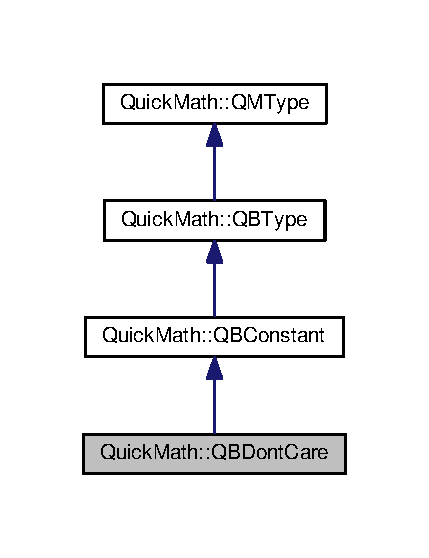
\includegraphics[width=206pt]{classQuickMath_1_1QBDontCare__inherit__graph}
\end{center}
\end{figure}


Collaboration diagram for Quick\+Math\+:\+:Q\+B\+Dont\+Care\+:
\nopagebreak
\begin{figure}[H]
\begin{center}
\leavevmode
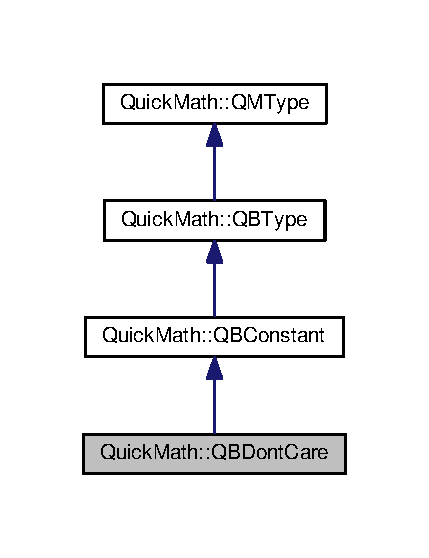
\includegraphics[width=206pt]{classQuickMath_1_1QBDontCare__coll__graph}
\end{center}
\end{figure}
\subsection*{Public Member Functions}
\begin{DoxyCompactItemize}
\item 
\hyperlink{namespaceQuickMath_aec13b08c42d9f8e688241623c8b379a0}{Q\+B\+Value} \hyperlink{classQuickMath_1_1QBDontCare_a40a7cfa35c7e91d392493277d3e5078e}{value} () const 
\item 
std\+::unique\+\_\+ptr$<$ \hyperlink{classQuickMath_1_1QMType}{Q\+M\+Type} $>$ \hyperlink{classQuickMath_1_1QBDontCare_a9faa0a15db6993b62efe04632dee9534}{clone} () const 
\end{DoxyCompactItemize}


\subsection{Member Function Documentation}
\hypertarget{classQuickMath_1_1QBDontCare_a9faa0a15db6993b62efe04632dee9534}{}\index{Quick\+Math\+::\+Q\+B\+Dont\+Care@{Quick\+Math\+::\+Q\+B\+Dont\+Care}!clone@{clone}}
\index{clone@{clone}!Quick\+Math\+::\+Q\+B\+Dont\+Care@{Quick\+Math\+::\+Q\+B\+Dont\+Care}}
\subsubsection[{clone}]{\setlength{\rightskip}{0pt plus 5cm}std\+::unique\+\_\+ptr$<$ {\bf Q\+M\+Type} $>$ Quick\+Math\+::\+Q\+B\+Dont\+Care\+::clone (
\begin{DoxyParamCaption}
{}
\end{DoxyParamCaption}
) const\hspace{0.3cm}{\ttfamily [virtual]}}\label{classQuickMath_1_1QBDontCare_a9faa0a15db6993b62efe04632dee9534}


Implements \hyperlink{classQuickMath_1_1QMType_a15b2a74a662417da99c6da9b7aaeff77}{Quick\+Math\+::\+Q\+M\+Type}.

\hypertarget{classQuickMath_1_1QBDontCare_a40a7cfa35c7e91d392493277d3e5078e}{}\index{Quick\+Math\+::\+Q\+B\+Dont\+Care@{Quick\+Math\+::\+Q\+B\+Dont\+Care}!value@{value}}
\index{value@{value}!Quick\+Math\+::\+Q\+B\+Dont\+Care@{Quick\+Math\+::\+Q\+B\+Dont\+Care}}
\subsubsection[{value}]{\setlength{\rightskip}{0pt plus 5cm}{\bf Q\+B\+Value} Quick\+Math\+::\+Q\+B\+Dont\+Care\+::value (
\begin{DoxyParamCaption}
{}
\end{DoxyParamCaption}
) const\hspace{0.3cm}{\ttfamily [virtual]}}\label{classQuickMath_1_1QBDontCare_a40a7cfa35c7e91d392493277d3e5078e}


Implements \hyperlink{classQuickMath_1_1QBConstant_a399a700088d6327765b88652cea43c0e}{Quick\+Math\+::\+Q\+B\+Constant}.



The documentation for this class was generated from the following files\+:\begin{DoxyCompactItemize}
\item 
include/\+Q\+Bool/\hyperlink{QBConstants_8h}{Q\+B\+Constants.\+h}\item 
src/\+Q\+Bool/\hyperlink{QBConstants_8cpp}{Q\+B\+Constants.\+cpp}\end{DoxyCompactItemize}

\hypertarget{classQuickMath_1_1QBExpr}{}\section{Quick\+Math\+:\+:Q\+B\+Expr Class Reference}
\label{classQuickMath_1_1QBExpr}\index{Quick\+Math\+::\+Q\+B\+Expr@{Quick\+Math\+::\+Q\+B\+Expr}}


{\ttfamily \#include $<$Q\+B\+Expr.\+h$>$}



Inheritance diagram for Quick\+Math\+:\+:Q\+B\+Expr\+:
\nopagebreak
\begin{figure}[H]
\begin{center}
\leavevmode
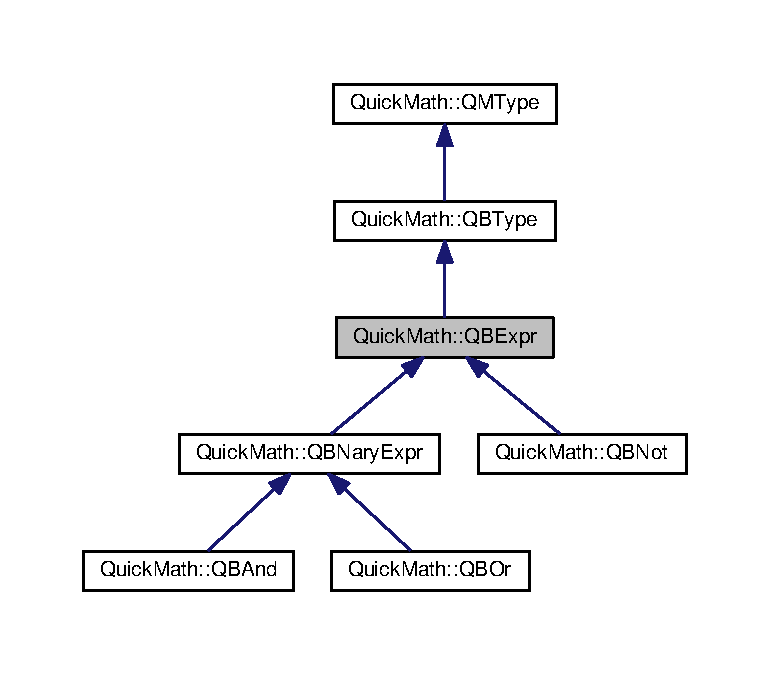
\includegraphics[width=350pt]{classQuickMath_1_1QBExpr__inherit__graph}
\end{center}
\end{figure}


Collaboration diagram for Quick\+Math\+:\+:Q\+B\+Expr\+:
\nopagebreak
\begin{figure}[H]
\begin{center}
\leavevmode
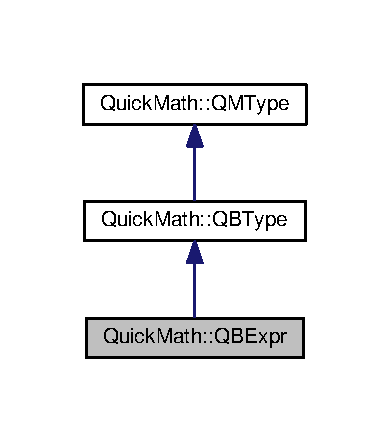
\includegraphics[width=187pt]{classQuickMath_1_1QBExpr__coll__graph}
\end{center}
\end{figure}
\subsection*{Public Member Functions}
\begin{DoxyCompactItemize}
\item 
virtual std\+::vector$<$ \hyperlink{namespaceQuickMath_af54af2708effd817452548da857ba076}{U\+Q\+B\+Type} $>$\+::iterator \hyperlink{classQuickMath_1_1QBExpr_a9f06f1ffed9764fe1ad22f2188bfd2e6}{begin} ()
\item 
virtual std\+::vector$<$ \hyperlink{namespaceQuickMath_af54af2708effd817452548da857ba076}{U\+Q\+B\+Type} $>$\+::iterator \hyperlink{classQuickMath_1_1QBExpr_a5ada70c2592cbd4f5fae81d675d52c5e}{end} ()
\item 
virtual std\+::vector$<$ \hyperlink{namespaceQuickMath_af54af2708effd817452548da857ba076}{U\+Q\+B\+Type} $>$\+::const\+\_\+iterator \hyperlink{classQuickMath_1_1QBExpr_a211c9edaff75febc84dd902ad3d3e110}{begin} () const 
\item 
virtual std\+::vector$<$ \hyperlink{namespaceQuickMath_af54af2708effd817452548da857ba076}{U\+Q\+B\+Type} $>$\+::const\+\_\+iterator \hyperlink{classQuickMath_1_1QBExpr_ab086e39434c516344e860457078dd529}{end} () const 
\item 
virtual unsigned int \hyperlink{classQuickMath_1_1QBExpr_a96b0038b62c74a0cb0d89885c0858168}{size} () const 
\item 
bool \hyperlink{classQuickMath_1_1QBExpr_a08e89c086e7cafce312c5766691a404a}{is\+Expr} () const 
\end{DoxyCompactItemize}
\subsection*{Protected Attributes}
\begin{DoxyCompactItemize}
\item 
std\+::vector$<$ \hyperlink{namespaceQuickMath_af54af2708effd817452548da857ba076}{U\+Q\+B\+Type} $>$ \hyperlink{classQuickMath_1_1QBExpr_ad3cff7ae0f5496d8e09990a66a395237}{operands}
\end{DoxyCompactItemize}


\subsection{Member Function Documentation}
\hypertarget{classQuickMath_1_1QBExpr_a9f06f1ffed9764fe1ad22f2188bfd2e6}{}\index{Quick\+Math\+::\+Q\+B\+Expr@{Quick\+Math\+::\+Q\+B\+Expr}!begin@{begin}}
\index{begin@{begin}!Quick\+Math\+::\+Q\+B\+Expr@{Quick\+Math\+::\+Q\+B\+Expr}}
\subsubsection[{begin}]{\setlength{\rightskip}{0pt plus 5cm}virtual std\+::vector$<${\bf U\+Q\+B\+Type}$>$\+::iterator Quick\+Math\+::\+Q\+B\+Expr\+::begin (
\begin{DoxyParamCaption}
{}
\end{DoxyParamCaption}
)\hspace{0.3cm}{\ttfamily [inline]}, {\ttfamily [virtual]}}\label{classQuickMath_1_1QBExpr_a9f06f1ffed9764fe1ad22f2188bfd2e6}
\hypertarget{classQuickMath_1_1QBExpr_a211c9edaff75febc84dd902ad3d3e110}{}\index{Quick\+Math\+::\+Q\+B\+Expr@{Quick\+Math\+::\+Q\+B\+Expr}!begin@{begin}}
\index{begin@{begin}!Quick\+Math\+::\+Q\+B\+Expr@{Quick\+Math\+::\+Q\+B\+Expr}}
\subsubsection[{begin}]{\setlength{\rightskip}{0pt plus 5cm}virtual std\+::vector$<${\bf U\+Q\+B\+Type}$>$\+::const\+\_\+iterator Quick\+Math\+::\+Q\+B\+Expr\+::begin (
\begin{DoxyParamCaption}
{}
\end{DoxyParamCaption}
) const\hspace{0.3cm}{\ttfamily [inline]}, {\ttfamily [virtual]}}\label{classQuickMath_1_1QBExpr_a211c9edaff75febc84dd902ad3d3e110}
\hypertarget{classQuickMath_1_1QBExpr_a5ada70c2592cbd4f5fae81d675d52c5e}{}\index{Quick\+Math\+::\+Q\+B\+Expr@{Quick\+Math\+::\+Q\+B\+Expr}!end@{end}}
\index{end@{end}!Quick\+Math\+::\+Q\+B\+Expr@{Quick\+Math\+::\+Q\+B\+Expr}}
\subsubsection[{end}]{\setlength{\rightskip}{0pt plus 5cm}virtual std\+::vector$<${\bf U\+Q\+B\+Type}$>$\+::iterator Quick\+Math\+::\+Q\+B\+Expr\+::end (
\begin{DoxyParamCaption}
{}
\end{DoxyParamCaption}
)\hspace{0.3cm}{\ttfamily [inline]}, {\ttfamily [virtual]}}\label{classQuickMath_1_1QBExpr_a5ada70c2592cbd4f5fae81d675d52c5e}
\hypertarget{classQuickMath_1_1QBExpr_ab086e39434c516344e860457078dd529}{}\index{Quick\+Math\+::\+Q\+B\+Expr@{Quick\+Math\+::\+Q\+B\+Expr}!end@{end}}
\index{end@{end}!Quick\+Math\+::\+Q\+B\+Expr@{Quick\+Math\+::\+Q\+B\+Expr}}
\subsubsection[{end}]{\setlength{\rightskip}{0pt plus 5cm}virtual std\+::vector$<${\bf U\+Q\+B\+Type}$>$\+::const\+\_\+iterator Quick\+Math\+::\+Q\+B\+Expr\+::end (
\begin{DoxyParamCaption}
{}
\end{DoxyParamCaption}
) const\hspace{0.3cm}{\ttfamily [inline]}, {\ttfamily [virtual]}}\label{classQuickMath_1_1QBExpr_ab086e39434c516344e860457078dd529}
\hypertarget{classQuickMath_1_1QBExpr_a08e89c086e7cafce312c5766691a404a}{}\index{Quick\+Math\+::\+Q\+B\+Expr@{Quick\+Math\+::\+Q\+B\+Expr}!is\+Expr@{is\+Expr}}
\index{is\+Expr@{is\+Expr}!Quick\+Math\+::\+Q\+B\+Expr@{Quick\+Math\+::\+Q\+B\+Expr}}
\subsubsection[{is\+Expr}]{\setlength{\rightskip}{0pt plus 5cm}bool Quick\+Math\+::\+Q\+B\+Expr\+::is\+Expr (
\begin{DoxyParamCaption}
{}
\end{DoxyParamCaption}
) const\hspace{0.3cm}{\ttfamily [inline]}, {\ttfamily [virtual]}}\label{classQuickMath_1_1QBExpr_a08e89c086e7cafce312c5766691a404a}


Reimplemented from \hyperlink{classQuickMath_1_1QBType_a773a28a659747ec2a5c13d2a6f401404}{Quick\+Math\+::\+Q\+B\+Type}.

\hypertarget{classQuickMath_1_1QBExpr_a96b0038b62c74a0cb0d89885c0858168}{}\index{Quick\+Math\+::\+Q\+B\+Expr@{Quick\+Math\+::\+Q\+B\+Expr}!size@{size}}
\index{size@{size}!Quick\+Math\+::\+Q\+B\+Expr@{Quick\+Math\+::\+Q\+B\+Expr}}
\subsubsection[{size}]{\setlength{\rightskip}{0pt plus 5cm}virtual unsigned int Quick\+Math\+::\+Q\+B\+Expr\+::size (
\begin{DoxyParamCaption}
{}
\end{DoxyParamCaption}
) const\hspace{0.3cm}{\ttfamily [inline]}, {\ttfamily [virtual]}}\label{classQuickMath_1_1QBExpr_a96b0038b62c74a0cb0d89885c0858168}


\subsection{Member Data Documentation}
\hypertarget{classQuickMath_1_1QBExpr_ad3cff7ae0f5496d8e09990a66a395237}{}\index{Quick\+Math\+::\+Q\+B\+Expr@{Quick\+Math\+::\+Q\+B\+Expr}!operands@{operands}}
\index{operands@{operands}!Quick\+Math\+::\+Q\+B\+Expr@{Quick\+Math\+::\+Q\+B\+Expr}}
\subsubsection[{operands}]{\setlength{\rightskip}{0pt plus 5cm}std\+::vector$<${\bf U\+Q\+B\+Type}$>$ Quick\+Math\+::\+Q\+B\+Expr\+::operands\hspace{0.3cm}{\ttfamily [protected]}}\label{classQuickMath_1_1QBExpr_ad3cff7ae0f5496d8e09990a66a395237}


The documentation for this class was generated from the following file\+:\begin{DoxyCompactItemize}
\item 
include/\+Q\+Bool/\hyperlink{QBExpr_8h}{Q\+B\+Expr.\+h}\end{DoxyCompactItemize}

\hypertarget{classQuickMath_1_1QBFunc}{}\section{Quick\+Math\+:\+:Q\+B\+Func Class Reference}
\label{classQuickMath_1_1QBFunc}\index{Quick\+Math\+::\+Q\+B\+Func@{Quick\+Math\+::\+Q\+B\+Func}}


{\ttfamily \#include $<$Q\+B\+Func.\+h$>$}

\subsection*{Public Member Functions}
\begin{DoxyCompactItemize}
\item 
\hyperlink{classQuickMath_1_1QBFunc_ab9f410bcd30f0096b51ddf2ecb4005f0}{Q\+B\+Func} ()=default
\item 
\hyperlink{classQuickMath_1_1QBFunc_abe40a3b2f47a147a3d6da555c058593b}{Q\+B\+Func} (std\+::unique\+\_\+ptr$<$ \hyperlink{classQuickMath_1_1QBType}{Q\+B\+Type} $>$ p\+Val)
\item 
\hyperlink{classQuickMath_1_1QBFunc_adca4b4fa0ce85f65c55d423a755af660}{Q\+B\+Func} (const \hyperlink{classQuickMath_1_1QBType}{Q\+B\+Type} $\ast$p\+Val)
\item 
\hyperlink{classQuickMath_1_1QBFunc_ac6ed36ac2f44e0c7e31df7838f6df9d6}{Q\+B\+Func} (bool val)
\item 
\hyperlink{classQuickMath_1_1QBFunc_a6e40b9a774151a60bd3821375376ea10}{Q\+B\+Func} (const \hyperlink{classQuickMath_1_1QBFunc}{Q\+B\+Func} \&func)
\item 
\hyperlink{classQuickMath_1_1QBFunc_a2938201b7b3e97644ececf58b040620a}{Q\+B\+Func} (\hyperlink{classQuickMath_1_1QBFunc}{Q\+B\+Func} \&\&func)
\item 
\hyperlink{classQuickMath_1_1QBFunc}{Q\+B\+Func} \hyperlink{classQuickMath_1_1QBFunc_a2161ea28eba3812d044c34ab4b4bce14}{operator=} (const \hyperlink{classQuickMath_1_1QBFunc}{Q\+B\+Func} \&func)
\item 
\hyperlink{classQuickMath_1_1QBFunc}{Q\+B\+Func} \& \hyperlink{classQuickMath_1_1QBFunc_a18fa3391066aba1c62ad8f29fe6a7c2b}{operator=} (\hyperlink{classQuickMath_1_1QBFunc}{Q\+B\+Func} \&\&func)
\item 
\hyperlink{classQuickMath_1_1QBFunc}{Q\+B\+Func} \& \hyperlink{classQuickMath_1_1QBFunc_a577c7d41b9b2ac1288b7f31a3cd2fda0}{operator\&=} (const \hyperlink{classQuickMath_1_1QBFunc}{Q\+B\+Func} \&func)
\item 
\hyperlink{classQuickMath_1_1QBFunc}{Q\+B\+Func} \& \hyperlink{classQuickMath_1_1QBFunc_abd44f26a6b8db3694a1caef95278220f}{operator\&=} (\hyperlink{classQuickMath_1_1QBFunc}{Q\+B\+Func} \&\&func)
\item 
\hyperlink{classQuickMath_1_1QBFunc}{Q\+B\+Func} \& \hyperlink{classQuickMath_1_1QBFunc_a830fc921fb1ca579bd174ce3477bb1b0}{operator$\vert$=} (\hyperlink{classQuickMath_1_1QBFunc}{Q\+B\+Func} \&\&func)
\item 
\hyperlink{classQuickMath_1_1QBFunc}{Q\+B\+Func} \& \hyperlink{classQuickMath_1_1QBFunc_a377042ac0c178a209c38603f4031952a}{operator$\vert$=} (const \hyperlink{classQuickMath_1_1QBFunc}{Q\+B\+Func} \&func)
\item 
\hyperlink{classQuickMath_1_1QBFunc}{Q\+B\+Func} \hyperlink{classQuickMath_1_1QBFunc_ad6a4a1ad9c0b1a157ffc2079b993e99c}{operator$\vert$=} (const \hyperlink{classQuickMath_1_1QBType}{Q\+B\+Type} \&func)
\item 
\hyperlink{namespaceQuickMath_aec13b08c42d9f8e688241623c8b379a0}{Q\+B\+Value} \hyperlink{classQuickMath_1_1QBFunc_a916d28b606961e501f417b507f8c8636}{evaluate} () const 
\item 
bool \hyperlink{classQuickMath_1_1QBFunc_aa9de5d9970a0045720c34e6bf3e302da}{is\+Expr} () const 
\item 
bool \hyperlink{classQuickMath_1_1QBFunc_a5eed8d5849a3374dd0eb054bb5b2df53}{is\+Var} () const 
\item 
const \hyperlink{classQuickMath_1_1QBType}{Q\+B\+Type} $\ast$ \hyperlink{classQuickMath_1_1QBFunc_aecfc380fec5a717235001086c614f13f}{get} () const 
\item 
\hyperlink{classQuickMath_1_1QBType}{Q\+B\+Type} $\ast$ \hyperlink{classQuickMath_1_1QBFunc_a9da6494f27c467275d1bf66c57e0871e}{get} ()
\item 
std\+::string \hyperlink{classQuickMath_1_1QBFunc_a2598989f19cf9260b93db7840bb87922}{to\+String} () const 
\end{DoxyCompactItemize}
\subsection*{Private Attributes}
\begin{DoxyCompactItemize}
\item 
\hyperlink{namespaceQuickMath_af54af2708effd817452548da857ba076}{U\+Q\+B\+Type} \hyperlink{classQuickMath_1_1QBFunc_af53f2f11b453fbb4e55310d9a34f5da2}{b\+Value}
\end{DoxyCompactItemize}
\subsection*{Friends}
\begin{DoxyCompactItemize}
\item 
\hyperlink{classQuickMath_1_1QBFunc}{Q\+B\+Func} \hyperlink{classQuickMath_1_1QBFunc_ab5ddbe52d9e3c77edaccf5dc984611c0}{operator$\vert$} (\hyperlink{classQuickMath_1_1QBFunc}{Q\+B\+Func} \&\&a\+Func, \hyperlink{classQuickMath_1_1QBFunc}{Q\+B\+Func} \&\&b\+Func)
\item 
\hyperlink{classQuickMath_1_1QBFunc}{Q\+B\+Func} \hyperlink{classQuickMath_1_1QBFunc_a4ffb75b9e72172624ef4ab5bba5f7f30}{operator$\vert$} (const \hyperlink{classQuickMath_1_1QBFunc}{Q\+B\+Func} \&a\+Func, \hyperlink{classQuickMath_1_1QBFunc}{Q\+B\+Func} \&\&b\+Func)
\item 
\hyperlink{classQuickMath_1_1QBFunc}{Q\+B\+Func} \hyperlink{classQuickMath_1_1QBFunc_a9076b9b85f7f2a91292956e80cbba9bc}{operator$\vert$} (\hyperlink{classQuickMath_1_1QBFunc}{Q\+B\+Func} \&\&a\+Func, const \hyperlink{classQuickMath_1_1QBFunc}{Q\+B\+Func} \&b\+Func)
\item 
\hyperlink{classQuickMath_1_1QBFunc}{Q\+B\+Func} \hyperlink{classQuickMath_1_1QBFunc_adc04fcf3b6ca182c537429de8b5503a3}{operator$\vert$} (const \hyperlink{classQuickMath_1_1QBFunc}{Q\+B\+Func} \&a\+Func, const \hyperlink{classQuickMath_1_1QBFunc}{Q\+B\+Func} \&b\+Func)
\item 
\hyperlink{classQuickMath_1_1QBFunc}{Q\+B\+Func} \hyperlink{classQuickMath_1_1QBFunc_a031286a681bc932973710fa5605099e3}{operator\&} (\hyperlink{classQuickMath_1_1QBFunc}{Q\+B\+Func} \&\&a\+Func, \hyperlink{classQuickMath_1_1QBFunc}{Q\+B\+Func} \&\&b\+Func)
\item 
\hyperlink{classQuickMath_1_1QBFunc}{Q\+B\+Func} \hyperlink{classQuickMath_1_1QBFunc_aeb45759e52c5c774050571a45103d512}{operator\&} (const \hyperlink{classQuickMath_1_1QBFunc}{Q\+B\+Func} \&a\+Func, \hyperlink{classQuickMath_1_1QBFunc}{Q\+B\+Func} \&\&b\+Func)
\item 
\hyperlink{classQuickMath_1_1QBFunc}{Q\+B\+Func} \hyperlink{classQuickMath_1_1QBFunc_a73bf3e8152a5065c9737541866334c94}{operator\&} (\hyperlink{classQuickMath_1_1QBFunc}{Q\+B\+Func} \&\&a\+Func, const \hyperlink{classQuickMath_1_1QBFunc}{Q\+B\+Func} \&b\+Func)
\item 
\hyperlink{classQuickMath_1_1QBFunc}{Q\+B\+Func} \hyperlink{classQuickMath_1_1QBFunc_a317711026cc82cd1a77e03c7b0c8dc4d}{operator\&} (const \hyperlink{classQuickMath_1_1QBFunc}{Q\+B\+Func} \&a\+Func, const \hyperlink{classQuickMath_1_1QBFunc}{Q\+B\+Func} \&b\+Func)
\item 
\hyperlink{classQuickMath_1_1QBFunc}{Q\+B\+Func} \hyperlink{classQuickMath_1_1QBFunc_ae7e0f0891f80732785ce12adff811f16}{operator!} (const \hyperlink{classQuickMath_1_1QBFunc}{Q\+B\+Func} \&func)
\item 
\hyperlink{classQuickMath_1_1QBFunc}{Q\+B\+Func} \hyperlink{classQuickMath_1_1QBFunc_ae22543f7ed9f2df4351f065afbc743b8}{operator!} (\hyperlink{classQuickMath_1_1QBFunc}{Q\+B\+Func} \&\&func)
\item 
\hyperlink{classQuickMath_1_1QBFunc}{Q\+B\+Func} \hyperlink{classQuickMath_1_1QBFunc_a7b66a9509b349058613309586610903a}{bi\+Conditional} (const \hyperlink{classQuickMath_1_1QBFunc}{Q\+B\+Func} \&antecedent, const \hyperlink{classQuickMath_1_1QBFunc}{Q\+B\+Func} \&consequent)
\item 
\hyperlink{classQuickMath_1_1QBFunc}{Q\+B\+Func} \hyperlink{classQuickMath_1_1QBFunc_afe30b33000c76760dc1dbcd9f9e02b6e}{implication} (const \hyperlink{classQuickMath_1_1QBFunc}{Q\+B\+Func} \&antecedent, const \hyperlink{classQuickMath_1_1QBFunc}{Q\+B\+Func} \&consequent)
\end{DoxyCompactItemize}


\subsection{Constructor \& Destructor Documentation}
\hypertarget{classQuickMath_1_1QBFunc_ab9f410bcd30f0096b51ddf2ecb4005f0}{}\index{Quick\+Math\+::\+Q\+B\+Func@{Quick\+Math\+::\+Q\+B\+Func}!Q\+B\+Func@{Q\+B\+Func}}
\index{Q\+B\+Func@{Q\+B\+Func}!Quick\+Math\+::\+Q\+B\+Func@{Quick\+Math\+::\+Q\+B\+Func}}
\subsubsection[{Q\+B\+Func}]{\setlength{\rightskip}{0pt plus 5cm}Quick\+Math\+::\+Q\+B\+Func\+::\+Q\+B\+Func (
\begin{DoxyParamCaption}
{}
\end{DoxyParamCaption}
)\hspace{0.3cm}{\ttfamily [default]}}\label{classQuickMath_1_1QBFunc_ab9f410bcd30f0096b51ddf2ecb4005f0}
\hypertarget{classQuickMath_1_1QBFunc_abe40a3b2f47a147a3d6da555c058593b}{}\index{Quick\+Math\+::\+Q\+B\+Func@{Quick\+Math\+::\+Q\+B\+Func}!Q\+B\+Func@{Q\+B\+Func}}
\index{Q\+B\+Func@{Q\+B\+Func}!Quick\+Math\+::\+Q\+B\+Func@{Quick\+Math\+::\+Q\+B\+Func}}
\subsubsection[{Q\+B\+Func}]{\setlength{\rightskip}{0pt plus 5cm}Quick\+Math\+::\+Q\+B\+Func\+::\+Q\+B\+Func (
\begin{DoxyParamCaption}
\item[{std\+::unique\+\_\+ptr$<$ {\bf Q\+B\+Type} $>$}]{p\+Val}
\end{DoxyParamCaption}
)}\label{classQuickMath_1_1QBFunc_abe40a3b2f47a147a3d6da555c058593b}
\hypertarget{classQuickMath_1_1QBFunc_adca4b4fa0ce85f65c55d423a755af660}{}\index{Quick\+Math\+::\+Q\+B\+Func@{Quick\+Math\+::\+Q\+B\+Func}!Q\+B\+Func@{Q\+B\+Func}}
\index{Q\+B\+Func@{Q\+B\+Func}!Quick\+Math\+::\+Q\+B\+Func@{Quick\+Math\+::\+Q\+B\+Func}}
\subsubsection[{Q\+B\+Func}]{\setlength{\rightskip}{0pt plus 5cm}Quick\+Math\+::\+Q\+B\+Func\+::\+Q\+B\+Func (
\begin{DoxyParamCaption}
\item[{const {\bf Q\+B\+Type} $\ast$}]{p\+Val}
\end{DoxyParamCaption}
)}\label{classQuickMath_1_1QBFunc_adca4b4fa0ce85f65c55d423a755af660}
\hypertarget{classQuickMath_1_1QBFunc_ac6ed36ac2f44e0c7e31df7838f6df9d6}{}\index{Quick\+Math\+::\+Q\+B\+Func@{Quick\+Math\+::\+Q\+B\+Func}!Q\+B\+Func@{Q\+B\+Func}}
\index{Q\+B\+Func@{Q\+B\+Func}!Quick\+Math\+::\+Q\+B\+Func@{Quick\+Math\+::\+Q\+B\+Func}}
\subsubsection[{Q\+B\+Func}]{\setlength{\rightskip}{0pt plus 5cm}Quick\+Math\+::\+Q\+B\+Func\+::\+Q\+B\+Func (
\begin{DoxyParamCaption}
\item[{bool}]{val}
\end{DoxyParamCaption}
)}\label{classQuickMath_1_1QBFunc_ac6ed36ac2f44e0c7e31df7838f6df9d6}
\hypertarget{classQuickMath_1_1QBFunc_a6e40b9a774151a60bd3821375376ea10}{}\index{Quick\+Math\+::\+Q\+B\+Func@{Quick\+Math\+::\+Q\+B\+Func}!Q\+B\+Func@{Q\+B\+Func}}
\index{Q\+B\+Func@{Q\+B\+Func}!Quick\+Math\+::\+Q\+B\+Func@{Quick\+Math\+::\+Q\+B\+Func}}
\subsubsection[{Q\+B\+Func}]{\setlength{\rightskip}{0pt plus 5cm}Quick\+Math\+::\+Q\+B\+Func\+::\+Q\+B\+Func (
\begin{DoxyParamCaption}
\item[{const {\bf Q\+B\+Func} \&}]{func}
\end{DoxyParamCaption}
)}\label{classQuickMath_1_1QBFunc_a6e40b9a774151a60bd3821375376ea10}
\hypertarget{classQuickMath_1_1QBFunc_a2938201b7b3e97644ececf58b040620a}{}\index{Quick\+Math\+::\+Q\+B\+Func@{Quick\+Math\+::\+Q\+B\+Func}!Q\+B\+Func@{Q\+B\+Func}}
\index{Q\+B\+Func@{Q\+B\+Func}!Quick\+Math\+::\+Q\+B\+Func@{Quick\+Math\+::\+Q\+B\+Func}}
\subsubsection[{Q\+B\+Func}]{\setlength{\rightskip}{0pt plus 5cm}Quick\+Math\+::\+Q\+B\+Func\+::\+Q\+B\+Func (
\begin{DoxyParamCaption}
\item[{{\bf Q\+B\+Func} \&\&}]{func}
\end{DoxyParamCaption}
)}\label{classQuickMath_1_1QBFunc_a2938201b7b3e97644ececf58b040620a}


\subsection{Member Function Documentation}
\hypertarget{classQuickMath_1_1QBFunc_a916d28b606961e501f417b507f8c8636}{}\index{Quick\+Math\+::\+Q\+B\+Func@{Quick\+Math\+::\+Q\+B\+Func}!evaluate@{evaluate}}
\index{evaluate@{evaluate}!Quick\+Math\+::\+Q\+B\+Func@{Quick\+Math\+::\+Q\+B\+Func}}
\subsubsection[{evaluate}]{\setlength{\rightskip}{0pt plus 5cm}{\bf Q\+B\+Value} Quick\+Math\+::\+Q\+B\+Func\+::evaluate (
\begin{DoxyParamCaption}
{}
\end{DoxyParamCaption}
) const}\label{classQuickMath_1_1QBFunc_a916d28b606961e501f417b507f8c8636}
\hypertarget{classQuickMath_1_1QBFunc_aecfc380fec5a717235001086c614f13f}{}\index{Quick\+Math\+::\+Q\+B\+Func@{Quick\+Math\+::\+Q\+B\+Func}!get@{get}}
\index{get@{get}!Quick\+Math\+::\+Q\+B\+Func@{Quick\+Math\+::\+Q\+B\+Func}}
\subsubsection[{get}]{\setlength{\rightskip}{0pt plus 5cm}const {\bf Q\+B\+Type} $\ast$ Quick\+Math\+::\+Q\+B\+Func\+::get (
\begin{DoxyParamCaption}
{}
\end{DoxyParamCaption}
) const}\label{classQuickMath_1_1QBFunc_aecfc380fec5a717235001086c614f13f}
\hypertarget{classQuickMath_1_1QBFunc_a9da6494f27c467275d1bf66c57e0871e}{}\index{Quick\+Math\+::\+Q\+B\+Func@{Quick\+Math\+::\+Q\+B\+Func}!get@{get}}
\index{get@{get}!Quick\+Math\+::\+Q\+B\+Func@{Quick\+Math\+::\+Q\+B\+Func}}
\subsubsection[{get}]{\setlength{\rightskip}{0pt plus 5cm}{\bf Q\+B\+Type} $\ast$ Quick\+Math\+::\+Q\+B\+Func\+::get (
\begin{DoxyParamCaption}
{}
\end{DoxyParamCaption}
)}\label{classQuickMath_1_1QBFunc_a9da6494f27c467275d1bf66c57e0871e}
\hypertarget{classQuickMath_1_1QBFunc_aa9de5d9970a0045720c34e6bf3e302da}{}\index{Quick\+Math\+::\+Q\+B\+Func@{Quick\+Math\+::\+Q\+B\+Func}!is\+Expr@{is\+Expr}}
\index{is\+Expr@{is\+Expr}!Quick\+Math\+::\+Q\+B\+Func@{Quick\+Math\+::\+Q\+B\+Func}}
\subsubsection[{is\+Expr}]{\setlength{\rightskip}{0pt plus 5cm}bool Quick\+Math\+::\+Q\+B\+Func\+::is\+Expr (
\begin{DoxyParamCaption}
{}
\end{DoxyParamCaption}
) const}\label{classQuickMath_1_1QBFunc_aa9de5d9970a0045720c34e6bf3e302da}
\hypertarget{classQuickMath_1_1QBFunc_a5eed8d5849a3374dd0eb054bb5b2df53}{}\index{Quick\+Math\+::\+Q\+B\+Func@{Quick\+Math\+::\+Q\+B\+Func}!is\+Var@{is\+Var}}
\index{is\+Var@{is\+Var}!Quick\+Math\+::\+Q\+B\+Func@{Quick\+Math\+::\+Q\+B\+Func}}
\subsubsection[{is\+Var}]{\setlength{\rightskip}{0pt plus 5cm}bool Quick\+Math\+::\+Q\+B\+Func\+::is\+Var (
\begin{DoxyParamCaption}
{}
\end{DoxyParamCaption}
) const}\label{classQuickMath_1_1QBFunc_a5eed8d5849a3374dd0eb054bb5b2df53}
\hypertarget{classQuickMath_1_1QBFunc_a577c7d41b9b2ac1288b7f31a3cd2fda0}{}\index{Quick\+Math\+::\+Q\+B\+Func@{Quick\+Math\+::\+Q\+B\+Func}!operator\&=@{operator\&=}}
\index{operator\&=@{operator\&=}!Quick\+Math\+::\+Q\+B\+Func@{Quick\+Math\+::\+Q\+B\+Func}}
\subsubsection[{operator\&=}]{\setlength{\rightskip}{0pt plus 5cm}{\bf Q\+B\+Func} \& Quick\+Math\+::\+Q\+B\+Func\+::operator\&= (
\begin{DoxyParamCaption}
\item[{const {\bf Q\+B\+Func} \&}]{func}
\end{DoxyParamCaption}
)}\label{classQuickMath_1_1QBFunc_a577c7d41b9b2ac1288b7f31a3cd2fda0}
\hypertarget{classQuickMath_1_1QBFunc_abd44f26a6b8db3694a1caef95278220f}{}\index{Quick\+Math\+::\+Q\+B\+Func@{Quick\+Math\+::\+Q\+B\+Func}!operator\&=@{operator\&=}}
\index{operator\&=@{operator\&=}!Quick\+Math\+::\+Q\+B\+Func@{Quick\+Math\+::\+Q\+B\+Func}}
\subsubsection[{operator\&=}]{\setlength{\rightskip}{0pt plus 5cm}{\bf Q\+B\+Func} \& Quick\+Math\+::\+Q\+B\+Func\+::operator\&= (
\begin{DoxyParamCaption}
\item[{{\bf Q\+B\+Func} \&\&}]{func}
\end{DoxyParamCaption}
)}\label{classQuickMath_1_1QBFunc_abd44f26a6b8db3694a1caef95278220f}
\hypertarget{classQuickMath_1_1QBFunc_a2161ea28eba3812d044c34ab4b4bce14}{}\index{Quick\+Math\+::\+Q\+B\+Func@{Quick\+Math\+::\+Q\+B\+Func}!operator=@{operator=}}
\index{operator=@{operator=}!Quick\+Math\+::\+Q\+B\+Func@{Quick\+Math\+::\+Q\+B\+Func}}
\subsubsection[{operator=}]{\setlength{\rightskip}{0pt plus 5cm}{\bf Q\+B\+Func} Quick\+Math\+::\+Q\+B\+Func\+::operator= (
\begin{DoxyParamCaption}
\item[{const {\bf Q\+B\+Func} \&}]{func}
\end{DoxyParamCaption}
)}\label{classQuickMath_1_1QBFunc_a2161ea28eba3812d044c34ab4b4bce14}
\hypertarget{classQuickMath_1_1QBFunc_a18fa3391066aba1c62ad8f29fe6a7c2b}{}\index{Quick\+Math\+::\+Q\+B\+Func@{Quick\+Math\+::\+Q\+B\+Func}!operator=@{operator=}}
\index{operator=@{operator=}!Quick\+Math\+::\+Q\+B\+Func@{Quick\+Math\+::\+Q\+B\+Func}}
\subsubsection[{operator=}]{\setlength{\rightskip}{0pt plus 5cm}{\bf Q\+B\+Func} \& Quick\+Math\+::\+Q\+B\+Func\+::operator= (
\begin{DoxyParamCaption}
\item[{{\bf Q\+B\+Func} \&\&}]{func}
\end{DoxyParamCaption}
)}\label{classQuickMath_1_1QBFunc_a18fa3391066aba1c62ad8f29fe6a7c2b}
\hypertarget{classQuickMath_1_1QBFunc_a830fc921fb1ca579bd174ce3477bb1b0}{}\index{Quick\+Math\+::\+Q\+B\+Func@{Quick\+Math\+::\+Q\+B\+Func}!operator\texttt{"|}=@{operator\texttt{"|}=}}
\index{operator\texttt{"|}=@{operator\texttt{"|}=}!Quick\+Math\+::\+Q\+B\+Func@{Quick\+Math\+::\+Q\+B\+Func}}
\subsubsection[{operator\texttt{"|}=}]{\setlength{\rightskip}{0pt plus 5cm}{\bf Q\+B\+Func} \& Quick\+Math\+::\+Q\+B\+Func\+::operator$\vert$= (
\begin{DoxyParamCaption}
\item[{{\bf Q\+B\+Func} \&\&}]{func}
\end{DoxyParamCaption}
)}\label{classQuickMath_1_1QBFunc_a830fc921fb1ca579bd174ce3477bb1b0}
\hypertarget{classQuickMath_1_1QBFunc_a377042ac0c178a209c38603f4031952a}{}\index{Quick\+Math\+::\+Q\+B\+Func@{Quick\+Math\+::\+Q\+B\+Func}!operator\texttt{"|}=@{operator\texttt{"|}=}}
\index{operator\texttt{"|}=@{operator\texttt{"|}=}!Quick\+Math\+::\+Q\+B\+Func@{Quick\+Math\+::\+Q\+B\+Func}}
\subsubsection[{operator\texttt{"|}=}]{\setlength{\rightskip}{0pt plus 5cm}{\bf Q\+B\+Func} \& Quick\+Math\+::\+Q\+B\+Func\+::operator$\vert$= (
\begin{DoxyParamCaption}
\item[{const {\bf Q\+B\+Func} \&}]{func}
\end{DoxyParamCaption}
)}\label{classQuickMath_1_1QBFunc_a377042ac0c178a209c38603f4031952a}
\hypertarget{classQuickMath_1_1QBFunc_ad6a4a1ad9c0b1a157ffc2079b993e99c}{}\index{Quick\+Math\+::\+Q\+B\+Func@{Quick\+Math\+::\+Q\+B\+Func}!operator\texttt{"|}=@{operator\texttt{"|}=}}
\index{operator\texttt{"|}=@{operator\texttt{"|}=}!Quick\+Math\+::\+Q\+B\+Func@{Quick\+Math\+::\+Q\+B\+Func}}
\subsubsection[{operator\texttt{"|}=}]{\setlength{\rightskip}{0pt plus 5cm}{\bf Q\+B\+Func} Quick\+Math\+::\+Q\+B\+Func\+::operator$\vert$= (
\begin{DoxyParamCaption}
\item[{const {\bf Q\+B\+Type} \&}]{func}
\end{DoxyParamCaption}
)}\label{classQuickMath_1_1QBFunc_ad6a4a1ad9c0b1a157ffc2079b993e99c}
\hypertarget{classQuickMath_1_1QBFunc_a2598989f19cf9260b93db7840bb87922}{}\index{Quick\+Math\+::\+Q\+B\+Func@{Quick\+Math\+::\+Q\+B\+Func}!to\+String@{to\+String}}
\index{to\+String@{to\+String}!Quick\+Math\+::\+Q\+B\+Func@{Quick\+Math\+::\+Q\+B\+Func}}
\subsubsection[{to\+String}]{\setlength{\rightskip}{0pt plus 5cm}std\+::string Quick\+Math\+::\+Q\+B\+Func\+::to\+String (
\begin{DoxyParamCaption}
{}
\end{DoxyParamCaption}
) const}\label{classQuickMath_1_1QBFunc_a2598989f19cf9260b93db7840bb87922}


\subsection{Friends And Related Function Documentation}
\hypertarget{classQuickMath_1_1QBFunc_a7b66a9509b349058613309586610903a}{}\index{Quick\+Math\+::\+Q\+B\+Func@{Quick\+Math\+::\+Q\+B\+Func}!bi\+Conditional@{bi\+Conditional}}
\index{bi\+Conditional@{bi\+Conditional}!Quick\+Math\+::\+Q\+B\+Func@{Quick\+Math\+::\+Q\+B\+Func}}
\subsubsection[{bi\+Conditional}]{\setlength{\rightskip}{0pt plus 5cm}{\bf Q\+B\+Func} bi\+Conditional (
\begin{DoxyParamCaption}
\item[{const {\bf Q\+B\+Func} \&}]{antecedent, }
\item[{const {\bf Q\+B\+Func} \&}]{consequent}
\end{DoxyParamCaption}
)\hspace{0.3cm}{\ttfamily [friend]}}\label{classQuickMath_1_1QBFunc_a7b66a9509b349058613309586610903a}
\hypertarget{classQuickMath_1_1QBFunc_afe30b33000c76760dc1dbcd9f9e02b6e}{}\index{Quick\+Math\+::\+Q\+B\+Func@{Quick\+Math\+::\+Q\+B\+Func}!implication@{implication}}
\index{implication@{implication}!Quick\+Math\+::\+Q\+B\+Func@{Quick\+Math\+::\+Q\+B\+Func}}
\subsubsection[{implication}]{\setlength{\rightskip}{0pt plus 5cm}{\bf Q\+B\+Func} implication (
\begin{DoxyParamCaption}
\item[{const {\bf Q\+B\+Func} \&}]{antecedent, }
\item[{const {\bf Q\+B\+Func} \&}]{consequent}
\end{DoxyParamCaption}
)\hspace{0.3cm}{\ttfamily [friend]}}\label{classQuickMath_1_1QBFunc_afe30b33000c76760dc1dbcd9f9e02b6e}
\hypertarget{classQuickMath_1_1QBFunc_ae7e0f0891f80732785ce12adff811f16}{}\index{Quick\+Math\+::\+Q\+B\+Func@{Quick\+Math\+::\+Q\+B\+Func}!operator"!@{operator"!}}
\index{operator"!@{operator"!}!Quick\+Math\+::\+Q\+B\+Func@{Quick\+Math\+::\+Q\+B\+Func}}
\subsubsection[{operator"!}]{\setlength{\rightskip}{0pt plus 5cm}{\bf Q\+B\+Func} operator! (
\begin{DoxyParamCaption}
\item[{const {\bf Q\+B\+Func} \&}]{func}
\end{DoxyParamCaption}
)\hspace{0.3cm}{\ttfamily [friend]}}\label{classQuickMath_1_1QBFunc_ae7e0f0891f80732785ce12adff811f16}
\hypertarget{classQuickMath_1_1QBFunc_ae22543f7ed9f2df4351f065afbc743b8}{}\index{Quick\+Math\+::\+Q\+B\+Func@{Quick\+Math\+::\+Q\+B\+Func}!operator"!@{operator"!}}
\index{operator"!@{operator"!}!Quick\+Math\+::\+Q\+B\+Func@{Quick\+Math\+::\+Q\+B\+Func}}
\subsubsection[{operator"!}]{\setlength{\rightskip}{0pt plus 5cm}{\bf Q\+B\+Func} operator! (
\begin{DoxyParamCaption}
\item[{{\bf Q\+B\+Func} \&\&}]{func}
\end{DoxyParamCaption}
)\hspace{0.3cm}{\ttfamily [friend]}}\label{classQuickMath_1_1QBFunc_ae22543f7ed9f2df4351f065afbc743b8}
\hypertarget{classQuickMath_1_1QBFunc_a031286a681bc932973710fa5605099e3}{}\index{Quick\+Math\+::\+Q\+B\+Func@{Quick\+Math\+::\+Q\+B\+Func}!operator\&@{operator\&}}
\index{operator\&@{operator\&}!Quick\+Math\+::\+Q\+B\+Func@{Quick\+Math\+::\+Q\+B\+Func}}
\subsubsection[{operator\&}]{\setlength{\rightskip}{0pt plus 5cm}{\bf Q\+B\+Func} operator\& (
\begin{DoxyParamCaption}
\item[{{\bf Q\+B\+Func} \&\&}]{a\+Func, }
\item[{{\bf Q\+B\+Func} \&\&}]{b\+Func}
\end{DoxyParamCaption}
)\hspace{0.3cm}{\ttfamily [friend]}}\label{classQuickMath_1_1QBFunc_a031286a681bc932973710fa5605099e3}
\hypertarget{classQuickMath_1_1QBFunc_aeb45759e52c5c774050571a45103d512}{}\index{Quick\+Math\+::\+Q\+B\+Func@{Quick\+Math\+::\+Q\+B\+Func}!operator\&@{operator\&}}
\index{operator\&@{operator\&}!Quick\+Math\+::\+Q\+B\+Func@{Quick\+Math\+::\+Q\+B\+Func}}
\subsubsection[{operator\&}]{\setlength{\rightskip}{0pt plus 5cm}{\bf Q\+B\+Func} operator\& (
\begin{DoxyParamCaption}
\item[{const {\bf Q\+B\+Func} \&}]{a\+Func, }
\item[{{\bf Q\+B\+Func} \&\&}]{b\+Func}
\end{DoxyParamCaption}
)\hspace{0.3cm}{\ttfamily [friend]}}\label{classQuickMath_1_1QBFunc_aeb45759e52c5c774050571a45103d512}
\hypertarget{classQuickMath_1_1QBFunc_a73bf3e8152a5065c9737541866334c94}{}\index{Quick\+Math\+::\+Q\+B\+Func@{Quick\+Math\+::\+Q\+B\+Func}!operator\&@{operator\&}}
\index{operator\&@{operator\&}!Quick\+Math\+::\+Q\+B\+Func@{Quick\+Math\+::\+Q\+B\+Func}}
\subsubsection[{operator\&}]{\setlength{\rightskip}{0pt plus 5cm}{\bf Q\+B\+Func} operator\& (
\begin{DoxyParamCaption}
\item[{{\bf Q\+B\+Func} \&\&}]{a\+Func, }
\item[{const {\bf Q\+B\+Func} \&}]{b\+Func}
\end{DoxyParamCaption}
)\hspace{0.3cm}{\ttfamily [friend]}}\label{classQuickMath_1_1QBFunc_a73bf3e8152a5065c9737541866334c94}
\hypertarget{classQuickMath_1_1QBFunc_a317711026cc82cd1a77e03c7b0c8dc4d}{}\index{Quick\+Math\+::\+Q\+B\+Func@{Quick\+Math\+::\+Q\+B\+Func}!operator\&@{operator\&}}
\index{operator\&@{operator\&}!Quick\+Math\+::\+Q\+B\+Func@{Quick\+Math\+::\+Q\+B\+Func}}
\subsubsection[{operator\&}]{\setlength{\rightskip}{0pt plus 5cm}{\bf Q\+B\+Func} operator\& (
\begin{DoxyParamCaption}
\item[{const {\bf Q\+B\+Func} \&}]{a\+Func, }
\item[{const {\bf Q\+B\+Func} \&}]{b\+Func}
\end{DoxyParamCaption}
)\hspace{0.3cm}{\ttfamily [friend]}}\label{classQuickMath_1_1QBFunc_a317711026cc82cd1a77e03c7b0c8dc4d}
\hypertarget{classQuickMath_1_1QBFunc_ab5ddbe52d9e3c77edaccf5dc984611c0}{}\index{Quick\+Math\+::\+Q\+B\+Func@{Quick\+Math\+::\+Q\+B\+Func}!operator\texttt{"|}@{operator\texttt{"|}}}
\index{operator\texttt{"|}@{operator\texttt{"|}}!Quick\+Math\+::\+Q\+B\+Func@{Quick\+Math\+::\+Q\+B\+Func}}
\subsubsection[{operator\texttt{"|}}]{\setlength{\rightskip}{0pt plus 5cm}{\bf Q\+B\+Func} operator$\vert$ (
\begin{DoxyParamCaption}
\item[{{\bf Q\+B\+Func} \&\&}]{a\+Func, }
\item[{{\bf Q\+B\+Func} \&\&}]{b\+Func}
\end{DoxyParamCaption}
)\hspace{0.3cm}{\ttfamily [friend]}}\label{classQuickMath_1_1QBFunc_ab5ddbe52d9e3c77edaccf5dc984611c0}
\hypertarget{classQuickMath_1_1QBFunc_a4ffb75b9e72172624ef4ab5bba5f7f30}{}\index{Quick\+Math\+::\+Q\+B\+Func@{Quick\+Math\+::\+Q\+B\+Func}!operator\texttt{"|}@{operator\texttt{"|}}}
\index{operator\texttt{"|}@{operator\texttt{"|}}!Quick\+Math\+::\+Q\+B\+Func@{Quick\+Math\+::\+Q\+B\+Func}}
\subsubsection[{operator\texttt{"|}}]{\setlength{\rightskip}{0pt plus 5cm}{\bf Q\+B\+Func} operator$\vert$ (
\begin{DoxyParamCaption}
\item[{const {\bf Q\+B\+Func} \&}]{a\+Func, }
\item[{{\bf Q\+B\+Func} \&\&}]{b\+Func}
\end{DoxyParamCaption}
)\hspace{0.3cm}{\ttfamily [friend]}}\label{classQuickMath_1_1QBFunc_a4ffb75b9e72172624ef4ab5bba5f7f30}
\hypertarget{classQuickMath_1_1QBFunc_a9076b9b85f7f2a91292956e80cbba9bc}{}\index{Quick\+Math\+::\+Q\+B\+Func@{Quick\+Math\+::\+Q\+B\+Func}!operator\texttt{"|}@{operator\texttt{"|}}}
\index{operator\texttt{"|}@{operator\texttt{"|}}!Quick\+Math\+::\+Q\+B\+Func@{Quick\+Math\+::\+Q\+B\+Func}}
\subsubsection[{operator\texttt{"|}}]{\setlength{\rightskip}{0pt plus 5cm}{\bf Q\+B\+Func} operator$\vert$ (
\begin{DoxyParamCaption}
\item[{{\bf Q\+B\+Func} \&\&}]{a\+Func, }
\item[{const {\bf Q\+B\+Func} \&}]{b\+Func}
\end{DoxyParamCaption}
)\hspace{0.3cm}{\ttfamily [friend]}}\label{classQuickMath_1_1QBFunc_a9076b9b85f7f2a91292956e80cbba9bc}
\hypertarget{classQuickMath_1_1QBFunc_adc04fcf3b6ca182c537429de8b5503a3}{}\index{Quick\+Math\+::\+Q\+B\+Func@{Quick\+Math\+::\+Q\+B\+Func}!operator\texttt{"|}@{operator\texttt{"|}}}
\index{operator\texttt{"|}@{operator\texttt{"|}}!Quick\+Math\+::\+Q\+B\+Func@{Quick\+Math\+::\+Q\+B\+Func}}
\subsubsection[{operator\texttt{"|}}]{\setlength{\rightskip}{0pt plus 5cm}{\bf Q\+B\+Func} operator$\vert$ (
\begin{DoxyParamCaption}
\item[{const {\bf Q\+B\+Func} \&}]{a\+Func, }
\item[{const {\bf Q\+B\+Func} \&}]{b\+Func}
\end{DoxyParamCaption}
)\hspace{0.3cm}{\ttfamily [friend]}}\label{classQuickMath_1_1QBFunc_adc04fcf3b6ca182c537429de8b5503a3}


\subsection{Member Data Documentation}
\hypertarget{classQuickMath_1_1QBFunc_af53f2f11b453fbb4e55310d9a34f5da2}{}\index{Quick\+Math\+::\+Q\+B\+Func@{Quick\+Math\+::\+Q\+B\+Func}!b\+Value@{b\+Value}}
\index{b\+Value@{b\+Value}!Quick\+Math\+::\+Q\+B\+Func@{Quick\+Math\+::\+Q\+B\+Func}}
\subsubsection[{b\+Value}]{\setlength{\rightskip}{0pt plus 5cm}{\bf U\+Q\+B\+Type} Quick\+Math\+::\+Q\+B\+Func\+::b\+Value\hspace{0.3cm}{\ttfamily [private]}}\label{classQuickMath_1_1QBFunc_af53f2f11b453fbb4e55310d9a34f5da2}


The documentation for this class was generated from the following files\+:\begin{DoxyCompactItemize}
\item 
include/\+Q\+Bool/\hyperlink{QBFunc_8h}{Q\+B\+Func.\+h}\item 
src/\+Q\+Bool/\hyperlink{QBFunc_8cpp}{Q\+B\+Func.\+cpp}\end{DoxyCompactItemize}

\hypertarget{classQuickMath_1_1QBinaryExpr}{}\section{Quick\+Math\+:\+:Q\+Binary\+Expr Class Reference}
\label{classQuickMath_1_1QBinaryExpr}\index{Quick\+Math\+::\+Q\+Binary\+Expr@{Quick\+Math\+::\+Q\+Binary\+Expr}}


{\ttfamily \#include $<$Q\+Binary\+Expr.\+h$>$}



Inheritance diagram for Quick\+Math\+:\+:Q\+Binary\+Expr\+:
\nopagebreak
\begin{figure}[H]
\begin{center}
\leavevmode
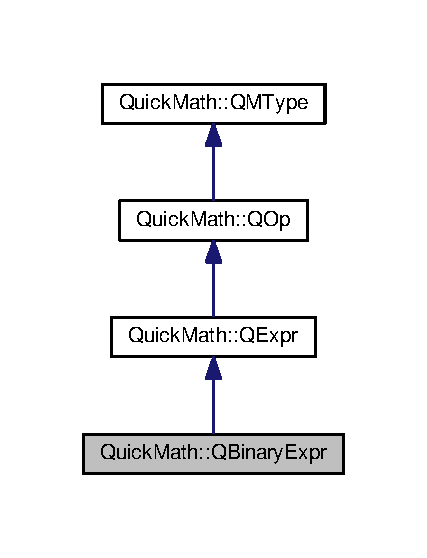
\includegraphics[width=205pt]{classQuickMath_1_1QBinaryExpr__inherit__graph}
\end{center}
\end{figure}


Collaboration diagram for Quick\+Math\+:\+:Q\+Binary\+Expr\+:
\nopagebreak
\begin{figure}[H]
\begin{center}
\leavevmode
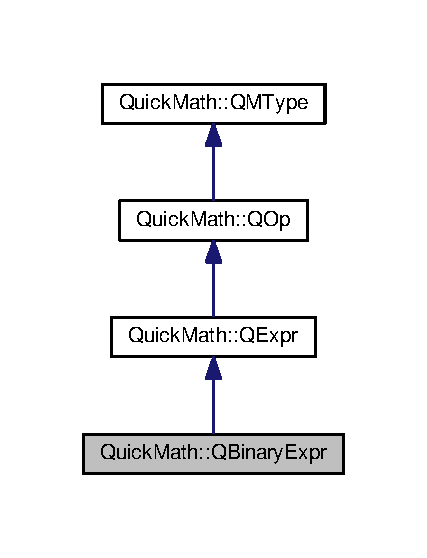
\includegraphics[width=205pt]{classQuickMath_1_1QBinaryExpr__coll__graph}
\end{center}
\end{figure}
\subsection*{Public Member Functions}
\begin{DoxyCompactItemize}
\item 
\hyperlink{classQuickMath_1_1QBinaryExpr_ae3e8ea0c221e7638af664ca6ce1f73bb}{Q\+Binary\+Expr} ()=default
\item 
\hyperlink{classQuickMath_1_1QBinaryExpr_a7d82ba57de6234fefe3becafa1537b80}{Q\+Binary\+Expr} (const \hyperlink{classQuickMath_1_1QBinaryExpr}{Q\+Binary\+Expr} \&other)
\item 
\hyperlink{classQuickMath_1_1QBinaryExpr_ad7bef4aa782a97b2a42e368dba19ed12}{Q\+Binary\+Expr} (\hyperlink{namespaceQuickMath_a0a6c67b9dab0cfd5f3e711b0573545cb}{Q\+M\+Op\+Type} type, std\+::unique\+\_\+ptr$<$ \hyperlink{classQuickMath_1_1QMType}{Q\+M\+Type} $>$ \&\&a, std\+::unique\+\_\+ptr$<$ \hyperlink{classQuickMath_1_1QMType}{Q\+M\+Type} $>$ \&\&b)
\item 
\hyperlink{classQuickMath_1_1QBinaryExpr_acd2a34c2332a67f3e00e56ab12b6e50f}{Q\+Binary\+Expr} (\hyperlink{namespaceQuickMath_a0a6c67b9dab0cfd5f3e711b0573545cb}{Q\+M\+Op\+Type} type, const \hyperlink{classQuickMath_1_1QMType}{Q\+M\+Type} \&a, const \hyperlink{classQuickMath_1_1QMType}{Q\+M\+Type} \&b)
\item 
\hyperlink{classQuickMath_1_1QBinaryExpr}{Q\+Binary\+Expr} \& \hyperlink{classQuickMath_1_1QBinaryExpr_a78895218c64c48c434bed0e80e732bcc}{operator=} (const \hyperlink{classQuickMath_1_1QBinaryExpr}{Q\+Binary\+Expr} \&other)
\item 
\hyperlink{classQuickMath_1_1QBinaryExpr}{Q\+Binary\+Expr} \& \hyperlink{classQuickMath_1_1QBinaryExpr_a0bc73ff4a6cd65d152c80a2259b4288b}{operator=} (\hyperlink{classQuickMath_1_1QBinaryExpr}{Q\+Binary\+Expr} \&\&other)
\item 
std\+::string \hyperlink{classQuickMath_1_1QBinaryExpr_ac253a522b55817ceeff36229d976dc79}{to\+String} () const 
\item 
const \hyperlink{classQuickMath_1_1QMType}{Q\+M\+Type} $\ast$ \hyperlink{classQuickMath_1_1QBinaryExpr_a89a08e6e8e83a664faafcb0ff984c94d}{left\+Operand} () const 
\item 
const \hyperlink{classQuickMath_1_1QMType}{Q\+M\+Type} $\ast$ \hyperlink{classQuickMath_1_1QBinaryExpr_a08d4732282c676dc8a57ee3bd2260a04}{right\+Operand} () const 
\item 
virtual std\+::array$<$ std\+::unique\+\_\+ptr$<$ \hyperlink{classQuickMath_1_1QMType}{Q\+M\+Type} $>$, 2 $>$\+::const\+\_\+iterator \hyperlink{classQuickMath_1_1QBinaryExpr_a28625c412a7c22d5c1060fa9f3db7877}{begin} () const 
\item 
virtual std\+::array$<$ std\+::unique\+\_\+ptr$<$ \hyperlink{classQuickMath_1_1QMType}{Q\+M\+Type} $>$, 2 $>$\+::const\+\_\+iterator \hyperlink{classQuickMath_1_1QBinaryExpr_a14f50114683fddb39cf74f2e82805672}{end} () const 
\item 
virtual std\+::unique\+\_\+ptr$<$ \hyperlink{classQuickMath_1_1QMType}{Q\+M\+Type} $>$ \hyperlink{classQuickMath_1_1QBinaryExpr_a1a13bf258ab921b56b63914b40a07909}{clone} () const 
\end{DoxyCompactItemize}
\subsection*{Protected Attributes}
\begin{DoxyCompactItemize}
\item 
std\+::array$<$ std\+::unique\+\_\+ptr$<$ \hyperlink{classQuickMath_1_1QMType}{Q\+M\+Type} $>$, 2 $>$ \hyperlink{classQuickMath_1_1QBinaryExpr_a9d788140e4b0eb6d635be7981bc8e60d}{operands}
\end{DoxyCompactItemize}


\subsection{Constructor \& Destructor Documentation}
\hypertarget{classQuickMath_1_1QBinaryExpr_ae3e8ea0c221e7638af664ca6ce1f73bb}{}\index{Quick\+Math\+::\+Q\+Binary\+Expr@{Quick\+Math\+::\+Q\+Binary\+Expr}!Q\+Binary\+Expr@{Q\+Binary\+Expr}}
\index{Q\+Binary\+Expr@{Q\+Binary\+Expr}!Quick\+Math\+::\+Q\+Binary\+Expr@{Quick\+Math\+::\+Q\+Binary\+Expr}}
\subsubsection[{Q\+Binary\+Expr}]{\setlength{\rightskip}{0pt plus 5cm}Quick\+Math\+::\+Q\+Binary\+Expr\+::\+Q\+Binary\+Expr (
\begin{DoxyParamCaption}
{}
\end{DoxyParamCaption}
)\hspace{0.3cm}{\ttfamily [default]}}\label{classQuickMath_1_1QBinaryExpr_ae3e8ea0c221e7638af664ca6ce1f73bb}
\hypertarget{classQuickMath_1_1QBinaryExpr_a7d82ba57de6234fefe3becafa1537b80}{}\index{Quick\+Math\+::\+Q\+Binary\+Expr@{Quick\+Math\+::\+Q\+Binary\+Expr}!Q\+Binary\+Expr@{Q\+Binary\+Expr}}
\index{Q\+Binary\+Expr@{Q\+Binary\+Expr}!Quick\+Math\+::\+Q\+Binary\+Expr@{Quick\+Math\+::\+Q\+Binary\+Expr}}
\subsubsection[{Q\+Binary\+Expr}]{\setlength{\rightskip}{0pt plus 5cm}Quick\+Math\+::\+Q\+Binary\+Expr\+::\+Q\+Binary\+Expr (
\begin{DoxyParamCaption}
\item[{const {\bf Q\+Binary\+Expr} \&}]{other}
\end{DoxyParamCaption}
)}\label{classQuickMath_1_1QBinaryExpr_a7d82ba57de6234fefe3becafa1537b80}
\hypertarget{classQuickMath_1_1QBinaryExpr_ad7bef4aa782a97b2a42e368dba19ed12}{}\index{Quick\+Math\+::\+Q\+Binary\+Expr@{Quick\+Math\+::\+Q\+Binary\+Expr}!Q\+Binary\+Expr@{Q\+Binary\+Expr}}
\index{Q\+Binary\+Expr@{Q\+Binary\+Expr}!Quick\+Math\+::\+Q\+Binary\+Expr@{Quick\+Math\+::\+Q\+Binary\+Expr}}
\subsubsection[{Q\+Binary\+Expr}]{\setlength{\rightskip}{0pt plus 5cm}Quick\+Math\+::\+Q\+Binary\+Expr\+::\+Q\+Binary\+Expr (
\begin{DoxyParamCaption}
\item[{{\bf Q\+M\+Op\+Type}}]{type, }
\item[{std\+::unique\+\_\+ptr$<$ {\bf Q\+M\+Type} $>$ \&\&}]{a, }
\item[{std\+::unique\+\_\+ptr$<$ {\bf Q\+M\+Type} $>$ \&\&}]{b}
\end{DoxyParamCaption}
)}\label{classQuickMath_1_1QBinaryExpr_ad7bef4aa782a97b2a42e368dba19ed12}
\hypertarget{classQuickMath_1_1QBinaryExpr_acd2a34c2332a67f3e00e56ab12b6e50f}{}\index{Quick\+Math\+::\+Q\+Binary\+Expr@{Quick\+Math\+::\+Q\+Binary\+Expr}!Q\+Binary\+Expr@{Q\+Binary\+Expr}}
\index{Q\+Binary\+Expr@{Q\+Binary\+Expr}!Quick\+Math\+::\+Q\+Binary\+Expr@{Quick\+Math\+::\+Q\+Binary\+Expr}}
\subsubsection[{Q\+Binary\+Expr}]{\setlength{\rightskip}{0pt plus 5cm}Quick\+Math\+::\+Q\+Binary\+Expr\+::\+Q\+Binary\+Expr (
\begin{DoxyParamCaption}
\item[{{\bf Q\+M\+Op\+Type}}]{type, }
\item[{const {\bf Q\+M\+Type} \&}]{a, }
\item[{const {\bf Q\+M\+Type} \&}]{b}
\end{DoxyParamCaption}
)}\label{classQuickMath_1_1QBinaryExpr_acd2a34c2332a67f3e00e56ab12b6e50f}


\subsection{Member Function Documentation}
\hypertarget{classQuickMath_1_1QBinaryExpr_a28625c412a7c22d5c1060fa9f3db7877}{}\index{Quick\+Math\+::\+Q\+Binary\+Expr@{Quick\+Math\+::\+Q\+Binary\+Expr}!begin@{begin}}
\index{begin@{begin}!Quick\+Math\+::\+Q\+Binary\+Expr@{Quick\+Math\+::\+Q\+Binary\+Expr}}
\subsubsection[{begin}]{\setlength{\rightskip}{0pt plus 5cm}std\+::array$<$ std\+::unique\+\_\+ptr$<$ {\bf Q\+M\+Type} $>$, 2 $>$\+::const\+\_\+iterator Quick\+Math\+::\+Q\+Binary\+Expr\+::begin (
\begin{DoxyParamCaption}
{}
\end{DoxyParamCaption}
) const\hspace{0.3cm}{\ttfamily [virtual]}}\label{classQuickMath_1_1QBinaryExpr_a28625c412a7c22d5c1060fa9f3db7877}
\hypertarget{classQuickMath_1_1QBinaryExpr_a1a13bf258ab921b56b63914b40a07909}{}\index{Quick\+Math\+::\+Q\+Binary\+Expr@{Quick\+Math\+::\+Q\+Binary\+Expr}!clone@{clone}}
\index{clone@{clone}!Quick\+Math\+::\+Q\+Binary\+Expr@{Quick\+Math\+::\+Q\+Binary\+Expr}}
\subsubsection[{clone}]{\setlength{\rightskip}{0pt plus 5cm}std\+::unique\+\_\+ptr$<$ {\bf Q\+M\+Type} $>$ Quick\+Math\+::\+Q\+Binary\+Expr\+::clone (
\begin{DoxyParamCaption}
{}
\end{DoxyParamCaption}
) const\hspace{0.3cm}{\ttfamily [virtual]}}\label{classQuickMath_1_1QBinaryExpr_a1a13bf258ab921b56b63914b40a07909}


Implements \hyperlink{classQuickMath_1_1QMType_a15b2a74a662417da99c6da9b7aaeff77}{Quick\+Math\+::\+Q\+M\+Type}.

\hypertarget{classQuickMath_1_1QBinaryExpr_a14f50114683fddb39cf74f2e82805672}{}\index{Quick\+Math\+::\+Q\+Binary\+Expr@{Quick\+Math\+::\+Q\+Binary\+Expr}!end@{end}}
\index{end@{end}!Quick\+Math\+::\+Q\+Binary\+Expr@{Quick\+Math\+::\+Q\+Binary\+Expr}}
\subsubsection[{end}]{\setlength{\rightskip}{0pt plus 5cm}std\+::array$<$ std\+::unique\+\_\+ptr$<$ {\bf Q\+M\+Type} $>$, 2 $>$\+::const\+\_\+iterator Quick\+Math\+::\+Q\+Binary\+Expr\+::end (
\begin{DoxyParamCaption}
{}
\end{DoxyParamCaption}
) const\hspace{0.3cm}{\ttfamily [virtual]}}\label{classQuickMath_1_1QBinaryExpr_a14f50114683fddb39cf74f2e82805672}
\hypertarget{classQuickMath_1_1QBinaryExpr_a89a08e6e8e83a664faafcb0ff984c94d}{}\index{Quick\+Math\+::\+Q\+Binary\+Expr@{Quick\+Math\+::\+Q\+Binary\+Expr}!left\+Operand@{left\+Operand}}
\index{left\+Operand@{left\+Operand}!Quick\+Math\+::\+Q\+Binary\+Expr@{Quick\+Math\+::\+Q\+Binary\+Expr}}
\subsubsection[{left\+Operand}]{\setlength{\rightskip}{0pt plus 5cm}const {\bf Q\+M\+Type} $\ast$ Quick\+Math\+::\+Q\+Binary\+Expr\+::left\+Operand (
\begin{DoxyParamCaption}
{}
\end{DoxyParamCaption}
) const}\label{classQuickMath_1_1QBinaryExpr_a89a08e6e8e83a664faafcb0ff984c94d}
\hypertarget{classQuickMath_1_1QBinaryExpr_a78895218c64c48c434bed0e80e732bcc}{}\index{Quick\+Math\+::\+Q\+Binary\+Expr@{Quick\+Math\+::\+Q\+Binary\+Expr}!operator=@{operator=}}
\index{operator=@{operator=}!Quick\+Math\+::\+Q\+Binary\+Expr@{Quick\+Math\+::\+Q\+Binary\+Expr}}
\subsubsection[{operator=}]{\setlength{\rightskip}{0pt plus 5cm}{\bf Q\+Binary\+Expr} \& Quick\+Math\+::\+Q\+Binary\+Expr\+::operator= (
\begin{DoxyParamCaption}
\item[{const {\bf Q\+Binary\+Expr} \&}]{other}
\end{DoxyParamCaption}
)}\label{classQuickMath_1_1QBinaryExpr_a78895218c64c48c434bed0e80e732bcc}
\hypertarget{classQuickMath_1_1QBinaryExpr_a0bc73ff4a6cd65d152c80a2259b4288b}{}\index{Quick\+Math\+::\+Q\+Binary\+Expr@{Quick\+Math\+::\+Q\+Binary\+Expr}!operator=@{operator=}}
\index{operator=@{operator=}!Quick\+Math\+::\+Q\+Binary\+Expr@{Quick\+Math\+::\+Q\+Binary\+Expr}}
\subsubsection[{operator=}]{\setlength{\rightskip}{0pt plus 5cm}{\bf Q\+Binary\+Expr} \& Quick\+Math\+::\+Q\+Binary\+Expr\+::operator= (
\begin{DoxyParamCaption}
\item[{{\bf Q\+Binary\+Expr} \&\&}]{other}
\end{DoxyParamCaption}
)}\label{classQuickMath_1_1QBinaryExpr_a0bc73ff4a6cd65d152c80a2259b4288b}
\hypertarget{classQuickMath_1_1QBinaryExpr_a08d4732282c676dc8a57ee3bd2260a04}{}\index{Quick\+Math\+::\+Q\+Binary\+Expr@{Quick\+Math\+::\+Q\+Binary\+Expr}!right\+Operand@{right\+Operand}}
\index{right\+Operand@{right\+Operand}!Quick\+Math\+::\+Q\+Binary\+Expr@{Quick\+Math\+::\+Q\+Binary\+Expr}}
\subsubsection[{right\+Operand}]{\setlength{\rightskip}{0pt plus 5cm}const {\bf Q\+M\+Type} $\ast$ Quick\+Math\+::\+Q\+Binary\+Expr\+::right\+Operand (
\begin{DoxyParamCaption}
{}
\end{DoxyParamCaption}
) const}\label{classQuickMath_1_1QBinaryExpr_a08d4732282c676dc8a57ee3bd2260a04}
\hypertarget{classQuickMath_1_1QBinaryExpr_ac253a522b55817ceeff36229d976dc79}{}\index{Quick\+Math\+::\+Q\+Binary\+Expr@{Quick\+Math\+::\+Q\+Binary\+Expr}!to\+String@{to\+String}}
\index{to\+String@{to\+String}!Quick\+Math\+::\+Q\+Binary\+Expr@{Quick\+Math\+::\+Q\+Binary\+Expr}}
\subsubsection[{to\+String}]{\setlength{\rightskip}{0pt plus 5cm}std\+::string Quick\+Math\+::\+Q\+Binary\+Expr\+::to\+String (
\begin{DoxyParamCaption}
{}
\end{DoxyParamCaption}
) const\hspace{0.3cm}{\ttfamily [virtual]}}\label{classQuickMath_1_1QBinaryExpr_ac253a522b55817ceeff36229d976dc79}


Implements \hyperlink{classQuickMath_1_1QMType_a031b83c87e4edae28c65adf8e268442b}{Quick\+Math\+::\+Q\+M\+Type}.



\subsection{Member Data Documentation}
\hypertarget{classQuickMath_1_1QBinaryExpr_a9d788140e4b0eb6d635be7981bc8e60d}{}\index{Quick\+Math\+::\+Q\+Binary\+Expr@{Quick\+Math\+::\+Q\+Binary\+Expr}!operands@{operands}}
\index{operands@{operands}!Quick\+Math\+::\+Q\+Binary\+Expr@{Quick\+Math\+::\+Q\+Binary\+Expr}}
\subsubsection[{operands}]{\setlength{\rightskip}{0pt plus 5cm}std\+::array$<$std\+::unique\+\_\+ptr$<${\bf Q\+M\+Type}$>$, 2$>$ Quick\+Math\+::\+Q\+Binary\+Expr\+::operands\hspace{0.3cm}{\ttfamily [protected]}}\label{classQuickMath_1_1QBinaryExpr_a9d788140e4b0eb6d635be7981bc8e60d}


The documentation for this class was generated from the following files\+:\begin{DoxyCompactItemize}
\item 
include/\+Q\+Mix/\hyperlink{QBinaryExpr_8h}{Q\+Binary\+Expr.\+h}\item 
src/\+Q\+Mix/\hyperlink{QBinaryExpr_8cpp}{Q\+Binary\+Expr.\+cpp}\end{DoxyCompactItemize}

\hypertarget{classQuickMath_1_1QBManager}{}\section{Quick\+Math\+:\+:Q\+B\+Manager Class Reference}
\label{classQuickMath_1_1QBManager}\index{Quick\+Math\+::\+Q\+B\+Manager@{Quick\+Math\+::\+Q\+B\+Manager}}


{\ttfamily \#include $<$Q\+B\+Manager.\+h$>$}

\subsection*{Classes}
\begin{DoxyCompactItemize}
\item 
struct \hyperlink{structQuickMath_1_1QBManager_1_1KeyPair}{Key\+Pair}
\end{DoxyCompactItemize}
\subsection*{Public Member Functions}
\begin{DoxyCompactItemize}
\item 
\hyperlink{classQuickMath_1_1QBManager_a732b5922caec8fefe2b343adc13bc04b}{Q\+B\+Manager} ()=default
\item 
\hyperlink{classQuickMath_1_1QBFunc}{Q\+B\+Func} \hyperlink{classQuickMath_1_1QBManager_add834cd3b142721a06844a206fa1bd6d}{get\+Bit} (const std\+::string \&name, int idx=0)
\item 
\hyperlink{classQuickMath_1_1QBVector}{Q\+B\+Vector} \hyperlink{classQuickMath_1_1QBManager_ac5ce2080c5adc4d69014059f6eb6f619}{get\+Bit\+Vector} (const std\+::string \&name, unsigned int size)
\item 
void \hyperlink{classQuickMath_1_1QBManager_ab2e146d1e4e93f80d8ba832e511f7042}{set\+Value} (\hyperlink{namespaceQuickMath_aec13b08c42d9f8e688241623c8b379a0}{Q\+B\+Value} val, const std\+::string \&name, int idx=0)
\item 
unsigned int \hyperlink{classQuickMath_1_1QBManager_ad45c81146ce1daf119529be6927ce8fd}{number\+Vars} () const 
\end{DoxyCompactItemize}
\subsection*{Private Attributes}
\begin{DoxyCompactItemize}
\item 
std\+::map$<$ \hyperlink{structQuickMath_1_1QBManager_1_1KeyPair}{Key\+Pair}, std\+::shared\+\_\+ptr$<$ \hyperlink{classQuickMath_1_1QBBitShared}{Q\+B\+Bit\+Shared} $>$ $>$ \hyperlink{classQuickMath_1_1QBManager_a0c6ad5951835017e18664c9ec10f67bd}{vars}
\end{DoxyCompactItemize}


\subsection{Constructor \& Destructor Documentation}
\hypertarget{classQuickMath_1_1QBManager_a732b5922caec8fefe2b343adc13bc04b}{}\index{Quick\+Math\+::\+Q\+B\+Manager@{Quick\+Math\+::\+Q\+B\+Manager}!Q\+B\+Manager@{Q\+B\+Manager}}
\index{Q\+B\+Manager@{Q\+B\+Manager}!Quick\+Math\+::\+Q\+B\+Manager@{Quick\+Math\+::\+Q\+B\+Manager}}
\subsubsection[{Q\+B\+Manager}]{\setlength{\rightskip}{0pt plus 5cm}Quick\+Math\+::\+Q\+B\+Manager\+::\+Q\+B\+Manager (
\begin{DoxyParamCaption}
{}
\end{DoxyParamCaption}
)\hspace{0.3cm}{\ttfamily [default]}}\label{classQuickMath_1_1QBManager_a732b5922caec8fefe2b343adc13bc04b}


\subsection{Member Function Documentation}
\hypertarget{classQuickMath_1_1QBManager_add834cd3b142721a06844a206fa1bd6d}{}\index{Quick\+Math\+::\+Q\+B\+Manager@{Quick\+Math\+::\+Q\+B\+Manager}!get\+Bit@{get\+Bit}}
\index{get\+Bit@{get\+Bit}!Quick\+Math\+::\+Q\+B\+Manager@{Quick\+Math\+::\+Q\+B\+Manager}}
\subsubsection[{get\+Bit}]{\setlength{\rightskip}{0pt plus 5cm}{\bf Q\+B\+Func} Quick\+Math\+::\+Q\+B\+Manager\+::get\+Bit (
\begin{DoxyParamCaption}
\item[{const std\+::string \&}]{name, }
\item[{int}]{idx = {\ttfamily 0}}
\end{DoxyParamCaption}
)}\label{classQuickMath_1_1QBManager_add834cd3b142721a06844a206fa1bd6d}
\hypertarget{classQuickMath_1_1QBManager_ac5ce2080c5adc4d69014059f6eb6f619}{}\index{Quick\+Math\+::\+Q\+B\+Manager@{Quick\+Math\+::\+Q\+B\+Manager}!get\+Bit\+Vector@{get\+Bit\+Vector}}
\index{get\+Bit\+Vector@{get\+Bit\+Vector}!Quick\+Math\+::\+Q\+B\+Manager@{Quick\+Math\+::\+Q\+B\+Manager}}
\subsubsection[{get\+Bit\+Vector}]{\setlength{\rightskip}{0pt plus 5cm}{\bf Q\+B\+Vector} Quick\+Math\+::\+Q\+B\+Manager\+::get\+Bit\+Vector (
\begin{DoxyParamCaption}
\item[{const std\+::string \&}]{name, }
\item[{unsigned int}]{size}
\end{DoxyParamCaption}
)}\label{classQuickMath_1_1QBManager_ac5ce2080c5adc4d69014059f6eb6f619}
\hypertarget{classQuickMath_1_1QBManager_ad45c81146ce1daf119529be6927ce8fd}{}\index{Quick\+Math\+::\+Q\+B\+Manager@{Quick\+Math\+::\+Q\+B\+Manager}!number\+Vars@{number\+Vars}}
\index{number\+Vars@{number\+Vars}!Quick\+Math\+::\+Q\+B\+Manager@{Quick\+Math\+::\+Q\+B\+Manager}}
\subsubsection[{number\+Vars}]{\setlength{\rightskip}{0pt plus 5cm}unsigned int Quick\+Math\+::\+Q\+B\+Manager\+::number\+Vars (
\begin{DoxyParamCaption}
{}
\end{DoxyParamCaption}
) const}\label{classQuickMath_1_1QBManager_ad45c81146ce1daf119529be6927ce8fd}
\hypertarget{classQuickMath_1_1QBManager_ab2e146d1e4e93f80d8ba832e511f7042}{}\index{Quick\+Math\+::\+Q\+B\+Manager@{Quick\+Math\+::\+Q\+B\+Manager}!set\+Value@{set\+Value}}
\index{set\+Value@{set\+Value}!Quick\+Math\+::\+Q\+B\+Manager@{Quick\+Math\+::\+Q\+B\+Manager}}
\subsubsection[{set\+Value}]{\setlength{\rightskip}{0pt plus 5cm}void Quick\+Math\+::\+Q\+B\+Manager\+::set\+Value (
\begin{DoxyParamCaption}
\item[{{\bf Q\+B\+Value}}]{val, }
\item[{const std\+::string \&}]{name, }
\item[{int}]{idx = {\ttfamily 0}}
\end{DoxyParamCaption}
)}\label{classQuickMath_1_1QBManager_ab2e146d1e4e93f80d8ba832e511f7042}


\subsection{Member Data Documentation}
\hypertarget{classQuickMath_1_1QBManager_a0c6ad5951835017e18664c9ec10f67bd}{}\index{Quick\+Math\+::\+Q\+B\+Manager@{Quick\+Math\+::\+Q\+B\+Manager}!vars@{vars}}
\index{vars@{vars}!Quick\+Math\+::\+Q\+B\+Manager@{Quick\+Math\+::\+Q\+B\+Manager}}
\subsubsection[{vars}]{\setlength{\rightskip}{0pt plus 5cm}std\+::map$<${\bf Key\+Pair}, std\+::shared\+\_\+ptr$<${\bf Q\+B\+Bit\+Shared}$>$ $>$ Quick\+Math\+::\+Q\+B\+Manager\+::vars\hspace{0.3cm}{\ttfamily [private]}}\label{classQuickMath_1_1QBManager_a0c6ad5951835017e18664c9ec10f67bd}


The documentation for this class was generated from the following files\+:\begin{DoxyCompactItemize}
\item 
include/\+Q\+Bool/\hyperlink{QBManager_8h}{Q\+B\+Manager.\+h}\item 
src/\+Q\+Bool/\hyperlink{QBManager_8cpp}{Q\+B\+Manager.\+cpp}\end{DoxyCompactItemize}

\hypertarget{classQuickMath_1_1QBNaryExpr}{}\section{Quick\+Math\+:\+:Q\+B\+Nary\+Expr Class Reference}
\label{classQuickMath_1_1QBNaryExpr}\index{Quick\+Math\+::\+Q\+B\+Nary\+Expr@{Quick\+Math\+::\+Q\+B\+Nary\+Expr}}


{\ttfamily \#include $<$Q\+B\+Nary\+Expr.\+h$>$}



Inheritance diagram for Quick\+Math\+:\+:Q\+B\+Nary\+Expr\+:
\nopagebreak
\begin{figure}[H]
\begin{center}
\leavevmode
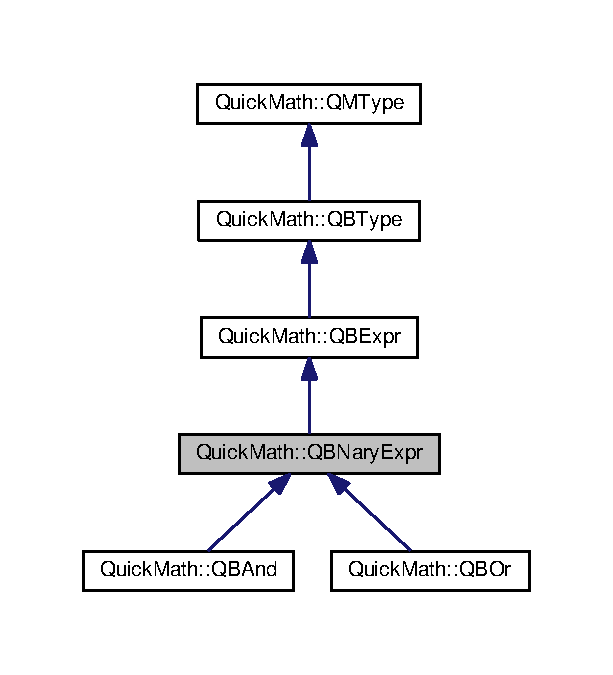
\includegraphics[width=294pt]{classQuickMath_1_1QBNaryExpr__inherit__graph}
\end{center}
\end{figure}


Collaboration diagram for Quick\+Math\+:\+:Q\+B\+Nary\+Expr\+:
\nopagebreak
\begin{figure}[H]
\begin{center}
\leavevmode
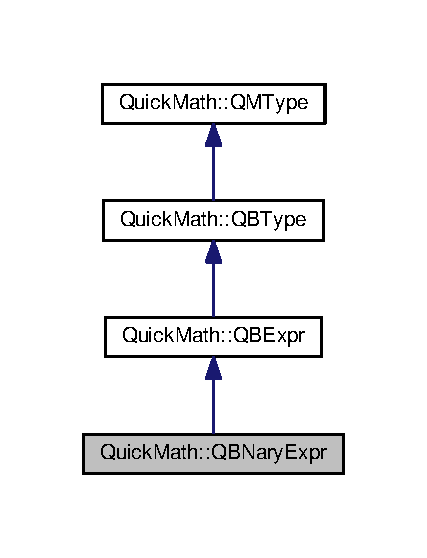
\includegraphics[width=205pt]{classQuickMath_1_1QBNaryExpr__coll__graph}
\end{center}
\end{figure}
\subsection*{Public Member Functions}
\begin{DoxyCompactItemize}
\item 
void \hyperlink{classQuickMath_1_1QBNaryExpr_ac213d52063e0a785bc7964783db6049a}{add\+Operand} (const \hyperlink{classQuickMath_1_1QBType}{Q\+B\+Type} \&func)
\item 
void \hyperlink{classQuickMath_1_1QBNaryExpr_a0499f0f103c0eae2bf39093dc4f74958}{add\+Operand} (\hyperlink{classQuickMath_1_1QBType}{Q\+B\+Type} \&\&func)
\end{DoxyCompactItemize}
\subsection*{Additional Inherited Members}


\subsection{Member Function Documentation}
\hypertarget{classQuickMath_1_1QBNaryExpr_ac213d52063e0a785bc7964783db6049a}{}\index{Quick\+Math\+::\+Q\+B\+Nary\+Expr@{Quick\+Math\+::\+Q\+B\+Nary\+Expr}!add\+Operand@{add\+Operand}}
\index{add\+Operand@{add\+Operand}!Quick\+Math\+::\+Q\+B\+Nary\+Expr@{Quick\+Math\+::\+Q\+B\+Nary\+Expr}}
\subsubsection[{add\+Operand}]{\setlength{\rightskip}{0pt plus 5cm}void Quick\+Math\+::\+Q\+B\+Nary\+Expr\+::add\+Operand (
\begin{DoxyParamCaption}
\item[{const {\bf Q\+B\+Type} \&}]{func}
\end{DoxyParamCaption}
)}\label{classQuickMath_1_1QBNaryExpr_ac213d52063e0a785bc7964783db6049a}
\hypertarget{classQuickMath_1_1QBNaryExpr_a0499f0f103c0eae2bf39093dc4f74958}{}\index{Quick\+Math\+::\+Q\+B\+Nary\+Expr@{Quick\+Math\+::\+Q\+B\+Nary\+Expr}!add\+Operand@{add\+Operand}}
\index{add\+Operand@{add\+Operand}!Quick\+Math\+::\+Q\+B\+Nary\+Expr@{Quick\+Math\+::\+Q\+B\+Nary\+Expr}}
\subsubsection[{add\+Operand}]{\setlength{\rightskip}{0pt plus 5cm}void Quick\+Math\+::\+Q\+B\+Nary\+Expr\+::add\+Operand (
\begin{DoxyParamCaption}
\item[{{\bf Q\+B\+Type} \&\&}]{func}
\end{DoxyParamCaption}
)}\label{classQuickMath_1_1QBNaryExpr_a0499f0f103c0eae2bf39093dc4f74958}


The documentation for this class was generated from the following files\+:\begin{DoxyCompactItemize}
\item 
include/\+Q\+Bool/\hyperlink{QBNaryExpr_8h}{Q\+B\+Nary\+Expr.\+h}\item 
src/\+Q\+Bool/\hyperlink{QBNaryExpr_8cpp}{Q\+B\+Nary\+Expr.\+cpp}\end{DoxyCompactItemize}

\hypertarget{classQuickMath_1_1QBNot}{}\section{Quick\+Math\+:\+:Q\+B\+Not Class Reference}
\label{classQuickMath_1_1QBNot}\index{Quick\+Math\+::\+Q\+B\+Not@{Quick\+Math\+::\+Q\+B\+Not}}


{\ttfamily \#include $<$Q\+B\+Not.\+h$>$}



Inheritance diagram for Quick\+Math\+:\+:Q\+B\+Not\+:
\nopagebreak
\begin{figure}[H]
\begin{center}
\leavevmode
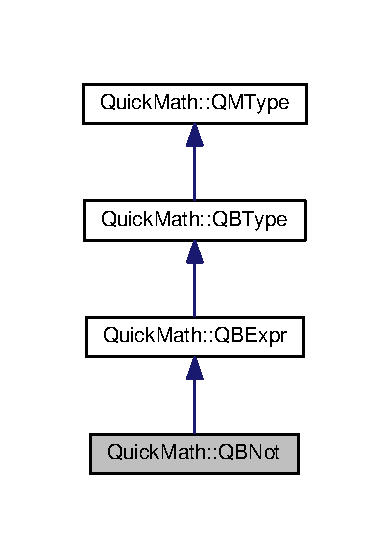
\includegraphics[width=187pt]{classQuickMath_1_1QBNot__inherit__graph}
\end{center}
\end{figure}


Collaboration diagram for Quick\+Math\+:\+:Q\+B\+Not\+:
\nopagebreak
\begin{figure}[H]
\begin{center}
\leavevmode
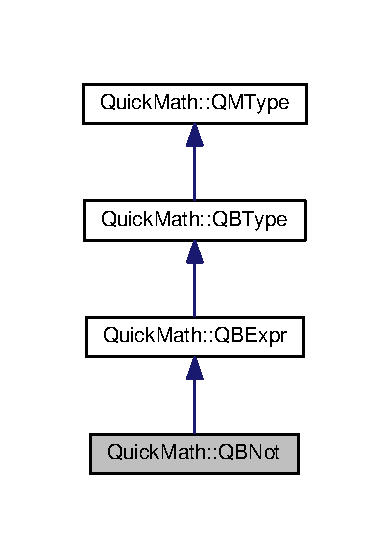
\includegraphics[width=187pt]{classQuickMath_1_1QBNot__coll__graph}
\end{center}
\end{figure}
\subsection*{Public Member Functions}
\begin{DoxyCompactItemize}
\item 
\hyperlink{classQuickMath_1_1QBNot_a105aa9b45a99277943f494fae83c72e4}{Q\+B\+Not} ()=default
\item 
\hyperlink{classQuickMath_1_1QBNot_abf0efd07e4cd81671abcc28046c55b2a}{Q\+B\+Not} (const \hyperlink{classQuickMath_1_1QBNot}{Q\+B\+Not} \&a)
\item 
\hyperlink{classQuickMath_1_1QBNot_a05f8d4a6031346145732d1beb23be454}{Q\+B\+Not} (\hyperlink{classQuickMath_1_1QBType}{Q\+B\+Type} \&a)
\item 
\hyperlink{classQuickMath_1_1QBNot_a1670154b87bae9f90ab7be2ccd9b7d99}{Q\+B\+Not} (std\+::unique\+\_\+ptr$<$ \hyperlink{classQuickMath_1_1QBType}{Q\+B\+Type} $>$ a)
\item 
std\+::string \hyperlink{classQuickMath_1_1QBNot_a946bcf1c86e2f59ea99537cb0fce2a80}{to\+String} () const 
\item 
\hyperlink{namespaceQuickMath_aec13b08c42d9f8e688241623c8b379a0}{Q\+B\+Value} \hyperlink{classQuickMath_1_1QBNot_a1b65e0c045a6ffb063a998b5751552d1}{value} () const 
\item 
std\+::unique\+\_\+ptr$<$ \hyperlink{classQuickMath_1_1QMType}{Q\+M\+Type} $>$ \hyperlink{classQuickMath_1_1QBNot_a89d67da57ae064f7ca0f38be07acce50}{clone} () const 
\item 
bool \hyperlink{classQuickMath_1_1QBNot_ab39947bbca2904d4678eef80dae58145}{is\+Not} () const 
\end{DoxyCompactItemize}
\subsection*{Additional Inherited Members}


\subsection{Constructor \& Destructor Documentation}
\hypertarget{classQuickMath_1_1QBNot_a105aa9b45a99277943f494fae83c72e4}{}\index{Quick\+Math\+::\+Q\+B\+Not@{Quick\+Math\+::\+Q\+B\+Not}!Q\+B\+Not@{Q\+B\+Not}}
\index{Q\+B\+Not@{Q\+B\+Not}!Quick\+Math\+::\+Q\+B\+Not@{Quick\+Math\+::\+Q\+B\+Not}}
\subsubsection[{Q\+B\+Not}]{\setlength{\rightskip}{0pt plus 5cm}Quick\+Math\+::\+Q\+B\+Not\+::\+Q\+B\+Not (
\begin{DoxyParamCaption}
{}
\end{DoxyParamCaption}
)\hspace{0.3cm}{\ttfamily [default]}}\label{classQuickMath_1_1QBNot_a105aa9b45a99277943f494fae83c72e4}
\hypertarget{classQuickMath_1_1QBNot_abf0efd07e4cd81671abcc28046c55b2a}{}\index{Quick\+Math\+::\+Q\+B\+Not@{Quick\+Math\+::\+Q\+B\+Not}!Q\+B\+Not@{Q\+B\+Not}}
\index{Q\+B\+Not@{Q\+B\+Not}!Quick\+Math\+::\+Q\+B\+Not@{Quick\+Math\+::\+Q\+B\+Not}}
\subsubsection[{Q\+B\+Not}]{\setlength{\rightskip}{0pt plus 5cm}Quick\+Math\+::\+Q\+B\+Not\+::\+Q\+B\+Not (
\begin{DoxyParamCaption}
\item[{const {\bf Q\+B\+Not} \&}]{a}
\end{DoxyParamCaption}
)}\label{classQuickMath_1_1QBNot_abf0efd07e4cd81671abcc28046c55b2a}
\hypertarget{classQuickMath_1_1QBNot_a05f8d4a6031346145732d1beb23be454}{}\index{Quick\+Math\+::\+Q\+B\+Not@{Quick\+Math\+::\+Q\+B\+Not}!Q\+B\+Not@{Q\+B\+Not}}
\index{Q\+B\+Not@{Q\+B\+Not}!Quick\+Math\+::\+Q\+B\+Not@{Quick\+Math\+::\+Q\+B\+Not}}
\subsubsection[{Q\+B\+Not}]{\setlength{\rightskip}{0pt plus 5cm}Quick\+Math\+::\+Q\+B\+Not\+::\+Q\+B\+Not (
\begin{DoxyParamCaption}
\item[{{\bf Q\+B\+Type} \&}]{a}
\end{DoxyParamCaption}
)}\label{classQuickMath_1_1QBNot_a05f8d4a6031346145732d1beb23be454}
\hypertarget{classQuickMath_1_1QBNot_a1670154b87bae9f90ab7be2ccd9b7d99}{}\index{Quick\+Math\+::\+Q\+B\+Not@{Quick\+Math\+::\+Q\+B\+Not}!Q\+B\+Not@{Q\+B\+Not}}
\index{Q\+B\+Not@{Q\+B\+Not}!Quick\+Math\+::\+Q\+B\+Not@{Quick\+Math\+::\+Q\+B\+Not}}
\subsubsection[{Q\+B\+Not}]{\setlength{\rightskip}{0pt plus 5cm}Quick\+Math\+::\+Q\+B\+Not\+::\+Q\+B\+Not (
\begin{DoxyParamCaption}
\item[{std\+::unique\+\_\+ptr$<$ {\bf Q\+B\+Type} $>$}]{a}
\end{DoxyParamCaption}
)}\label{classQuickMath_1_1QBNot_a1670154b87bae9f90ab7be2ccd9b7d99}


\subsection{Member Function Documentation}
\hypertarget{classQuickMath_1_1QBNot_a89d67da57ae064f7ca0f38be07acce50}{}\index{Quick\+Math\+::\+Q\+B\+Not@{Quick\+Math\+::\+Q\+B\+Not}!clone@{clone}}
\index{clone@{clone}!Quick\+Math\+::\+Q\+B\+Not@{Quick\+Math\+::\+Q\+B\+Not}}
\subsubsection[{clone}]{\setlength{\rightskip}{0pt plus 5cm}std\+::unique\+\_\+ptr$<$ {\bf Q\+M\+Type} $>$ Quick\+Math\+::\+Q\+B\+Not\+::clone (
\begin{DoxyParamCaption}
{}
\end{DoxyParamCaption}
) const\hspace{0.3cm}{\ttfamily [virtual]}}\label{classQuickMath_1_1QBNot_a89d67da57ae064f7ca0f38be07acce50}


Implements \hyperlink{classQuickMath_1_1QMType_a15b2a74a662417da99c6da9b7aaeff77}{Quick\+Math\+::\+Q\+M\+Type}.

\hypertarget{classQuickMath_1_1QBNot_ab39947bbca2904d4678eef80dae58145}{}\index{Quick\+Math\+::\+Q\+B\+Not@{Quick\+Math\+::\+Q\+B\+Not}!is\+Not@{is\+Not}}
\index{is\+Not@{is\+Not}!Quick\+Math\+::\+Q\+B\+Not@{Quick\+Math\+::\+Q\+B\+Not}}
\subsubsection[{is\+Not}]{\setlength{\rightskip}{0pt plus 5cm}bool Quick\+Math\+::\+Q\+B\+Not\+::is\+Not (
\begin{DoxyParamCaption}
{}
\end{DoxyParamCaption}
) const\hspace{0.3cm}{\ttfamily [virtual]}}\label{classQuickMath_1_1QBNot_ab39947bbca2904d4678eef80dae58145}


Reimplemented from \hyperlink{classQuickMath_1_1QBType_a34cdcf8324b2091eae169992c1fcfa5b}{Quick\+Math\+::\+Q\+B\+Type}.

\hypertarget{classQuickMath_1_1QBNot_a946bcf1c86e2f59ea99537cb0fce2a80}{}\index{Quick\+Math\+::\+Q\+B\+Not@{Quick\+Math\+::\+Q\+B\+Not}!to\+String@{to\+String}}
\index{to\+String@{to\+String}!Quick\+Math\+::\+Q\+B\+Not@{Quick\+Math\+::\+Q\+B\+Not}}
\subsubsection[{to\+String}]{\setlength{\rightskip}{0pt plus 5cm}std\+::string Quick\+Math\+::\+Q\+B\+Not\+::to\+String (
\begin{DoxyParamCaption}
{}
\end{DoxyParamCaption}
) const\hspace{0.3cm}{\ttfamily [virtual]}}\label{classQuickMath_1_1QBNot_a946bcf1c86e2f59ea99537cb0fce2a80}


Implements \hyperlink{classQuickMath_1_1QBType_a12a08061a73649a9f79995469f8297d2}{Quick\+Math\+::\+Q\+B\+Type}.

\hypertarget{classQuickMath_1_1QBNot_a1b65e0c045a6ffb063a998b5751552d1}{}\index{Quick\+Math\+::\+Q\+B\+Not@{Quick\+Math\+::\+Q\+B\+Not}!value@{value}}
\index{value@{value}!Quick\+Math\+::\+Q\+B\+Not@{Quick\+Math\+::\+Q\+B\+Not}}
\subsubsection[{value}]{\setlength{\rightskip}{0pt plus 5cm}{\bf Q\+B\+Value} Quick\+Math\+::\+Q\+B\+Not\+::value (
\begin{DoxyParamCaption}
{}
\end{DoxyParamCaption}
) const\hspace{0.3cm}{\ttfamily [virtual]}}\label{classQuickMath_1_1QBNot_a1b65e0c045a6ffb063a998b5751552d1}


Implements \hyperlink{classQuickMath_1_1QBType_a3fa2589c7d1fa4a52e79193bef845eeb}{Quick\+Math\+::\+Q\+B\+Type}.



The documentation for this class was generated from the following files\+:\begin{DoxyCompactItemize}
\item 
include/\+Q\+Bool/\hyperlink{QBNot_8h}{Q\+B\+Not.\+h}\item 
src/\+Q\+Bool/\hyperlink{QBNot_8cpp}{Q\+B\+Not.\+cpp}\end{DoxyCompactItemize}

\hypertarget{classQuickMath_1_1QBOne}{}\section{Quick\+Math\+:\+:Q\+B\+One Class Reference}
\label{classQuickMath_1_1QBOne}\index{Quick\+Math\+::\+Q\+B\+One@{Quick\+Math\+::\+Q\+B\+One}}


{\ttfamily \#include $<$Q\+B\+Constants.\+h$>$}



Inheritance diagram for Quick\+Math\+:\+:Q\+B\+One\+:
\nopagebreak
\begin{figure}[H]
\begin{center}
\leavevmode
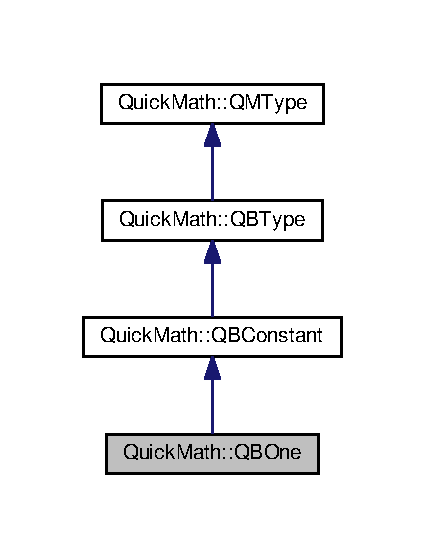
\includegraphics[width=204pt]{classQuickMath_1_1QBOne__inherit__graph}
\end{center}
\end{figure}


Collaboration diagram for Quick\+Math\+:\+:Q\+B\+One\+:
\nopagebreak
\begin{figure}[H]
\begin{center}
\leavevmode
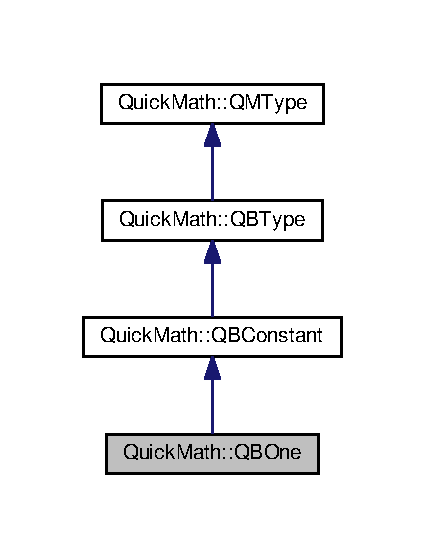
\includegraphics[width=204pt]{classQuickMath_1_1QBOne__coll__graph}
\end{center}
\end{figure}
\subsection*{Public Member Functions}
\begin{DoxyCompactItemize}
\item 
\hyperlink{namespaceQuickMath_aec13b08c42d9f8e688241623c8b379a0}{Q\+B\+Value} \hyperlink{classQuickMath_1_1QBOne_a2cc8ebd48be0d6edbfe0356d54d14919}{value} () const 
\item 
std\+::unique\+\_\+ptr$<$ \hyperlink{classQuickMath_1_1QMType}{Q\+M\+Type} $>$ \hyperlink{classQuickMath_1_1QBOne_ad6247a6496a23cc7025434149d7116fd}{clone} () const 
\item 
bool \hyperlink{classQuickMath_1_1QBOne_a2feb41d768849c7e1cc16a64898a2151}{is\+One} () const 
\end{DoxyCompactItemize}


\subsection{Member Function Documentation}
\hypertarget{classQuickMath_1_1QBOne_ad6247a6496a23cc7025434149d7116fd}{}\index{Quick\+Math\+::\+Q\+B\+One@{Quick\+Math\+::\+Q\+B\+One}!clone@{clone}}
\index{clone@{clone}!Quick\+Math\+::\+Q\+B\+One@{Quick\+Math\+::\+Q\+B\+One}}
\subsubsection[{clone}]{\setlength{\rightskip}{0pt plus 5cm}std\+::unique\+\_\+ptr$<$ {\bf Q\+M\+Type} $>$ Quick\+Math\+::\+Q\+B\+One\+::clone (
\begin{DoxyParamCaption}
{}
\end{DoxyParamCaption}
) const\hspace{0.3cm}{\ttfamily [virtual]}}\label{classQuickMath_1_1QBOne_ad6247a6496a23cc7025434149d7116fd}


Implements \hyperlink{classQuickMath_1_1QMType_a15b2a74a662417da99c6da9b7aaeff77}{Quick\+Math\+::\+Q\+M\+Type}.

\hypertarget{classQuickMath_1_1QBOne_a2feb41d768849c7e1cc16a64898a2151}{}\index{Quick\+Math\+::\+Q\+B\+One@{Quick\+Math\+::\+Q\+B\+One}!is\+One@{is\+One}}
\index{is\+One@{is\+One}!Quick\+Math\+::\+Q\+B\+One@{Quick\+Math\+::\+Q\+B\+One}}
\subsubsection[{is\+One}]{\setlength{\rightskip}{0pt plus 5cm}bool Quick\+Math\+::\+Q\+B\+One\+::is\+One (
\begin{DoxyParamCaption}
{}
\end{DoxyParamCaption}
) const\hspace{0.3cm}{\ttfamily [virtual]}}\label{classQuickMath_1_1QBOne_a2feb41d768849c7e1cc16a64898a2151}


Reimplemented from \hyperlink{classQuickMath_1_1QBType_acf934f5d9bc0974db2ca1294b3d2f864}{Quick\+Math\+::\+Q\+B\+Type}.

\hypertarget{classQuickMath_1_1QBOne_a2cc8ebd48be0d6edbfe0356d54d14919}{}\index{Quick\+Math\+::\+Q\+B\+One@{Quick\+Math\+::\+Q\+B\+One}!value@{value}}
\index{value@{value}!Quick\+Math\+::\+Q\+B\+One@{Quick\+Math\+::\+Q\+B\+One}}
\subsubsection[{value}]{\setlength{\rightskip}{0pt plus 5cm}{\bf Q\+B\+Value} Quick\+Math\+::\+Q\+B\+One\+::value (
\begin{DoxyParamCaption}
{}
\end{DoxyParamCaption}
) const\hspace{0.3cm}{\ttfamily [virtual]}}\label{classQuickMath_1_1QBOne_a2cc8ebd48be0d6edbfe0356d54d14919}


Implements \hyperlink{classQuickMath_1_1QBConstant_a399a700088d6327765b88652cea43c0e}{Quick\+Math\+::\+Q\+B\+Constant}.



The documentation for this class was generated from the following files\+:\begin{DoxyCompactItemize}
\item 
include/\+Q\+Bool/\hyperlink{QBConstants_8h}{Q\+B\+Constants.\+h}\item 
src/\+Q\+Bool/\hyperlink{QBConstants_8cpp}{Q\+B\+Constants.\+cpp}\end{DoxyCompactItemize}

\hypertarget{classQuickMath_1_1QBOr}{}\section{Quick\+Math\+:\+:Q\+B\+Or Class Reference}
\label{classQuickMath_1_1QBOr}\index{Quick\+Math\+::\+Q\+B\+Or@{Quick\+Math\+::\+Q\+B\+Or}}


{\ttfamily \#include $<$Q\+B\+Or.\+h$>$}



Inheritance diagram for Quick\+Math\+:\+:Q\+B\+Or\+:
\nopagebreak
\begin{figure}[H]
\begin{center}
\leavevmode
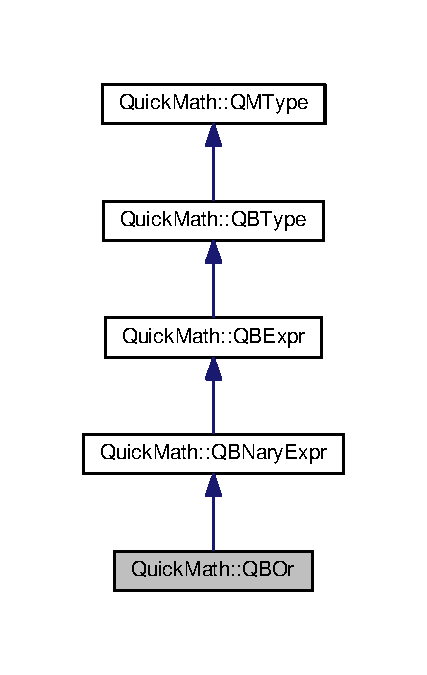
\includegraphics[width=205pt]{classQuickMath_1_1QBOr__inherit__graph}
\end{center}
\end{figure}


Collaboration diagram for Quick\+Math\+:\+:Q\+B\+Or\+:
\nopagebreak
\begin{figure}[H]
\begin{center}
\leavevmode
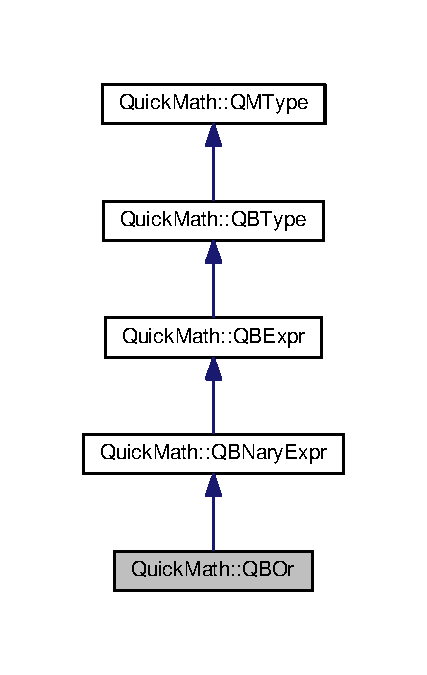
\includegraphics[width=205pt]{classQuickMath_1_1QBOr__coll__graph}
\end{center}
\end{figure}
\subsection*{Public Member Functions}
\begin{DoxyCompactItemize}
\item 
\hyperlink{classQuickMath_1_1QBOr_aaae4140dc674df41797504cacb9eb24f}{Q\+B\+Or} ()=default
\item 
\hyperlink{classQuickMath_1_1QBOr_ae02fedbf26450dabb879ca86f0cfda96}{Q\+B\+Or} (std\+::unique\+\_\+ptr$<$ \hyperlink{classQuickMath_1_1QBType}{Q\+B\+Type} $>$ a, const \hyperlink{classQuickMath_1_1QBType}{Q\+B\+Type} \&b)
\item 
\hyperlink{classQuickMath_1_1QBOr_a7f092c34224329a48ac9ea697200744f}{Q\+B\+Or} (const \hyperlink{classQuickMath_1_1QBType}{Q\+B\+Type} \&a, std\+::unique\+\_\+ptr$<$ \hyperlink{classQuickMath_1_1QBType}{Q\+B\+Type} $>$ b)
\item 
\hyperlink{classQuickMath_1_1QBOr_a07a3f4f70492e1c1c994e59c96ebaa6b}{Q\+B\+Or} (std\+::unique\+\_\+ptr$<$ \hyperlink{classQuickMath_1_1QBType}{Q\+B\+Type} $>$ a, std\+::unique\+\_\+ptr$<$ \hyperlink{classQuickMath_1_1QBType}{Q\+B\+Type} $>$ b)
\item 
\hyperlink{classQuickMath_1_1QBOr_a061922981120c55cff4ac1ee0b0abeb4}{Q\+B\+Or} (const \hyperlink{classQuickMath_1_1QBType}{Q\+B\+Type} \&a, const \hyperlink{classQuickMath_1_1QBType}{Q\+B\+Type} \&b)
\item 
\hyperlink{classQuickMath_1_1QBOr_af6f38dbcafdfbca22cefd966fc5deca8}{Q\+B\+Or} (const \hyperlink{classQuickMath_1_1QBOr}{Q\+B\+Or} \&other)
\item 
std\+::string \hyperlink{classQuickMath_1_1QBOr_ae835a7fda64bca20388ff3a869a9c928}{to\+String} () const 
\item 
\hyperlink{namespaceQuickMath_aec13b08c42d9f8e688241623c8b379a0}{Q\+B\+Value} \hyperlink{classQuickMath_1_1QBOr_a385b6b29141e89e46629da29a8e38c8f}{value} () const 
\item 
std\+::unique\+\_\+ptr$<$ \hyperlink{classQuickMath_1_1QMType}{Q\+M\+Type} $>$ \hyperlink{classQuickMath_1_1QBOr_af1ef65aaf163785db31aefa43253cb6c}{clone} () const 
\item 
bool \hyperlink{classQuickMath_1_1QBOr_ab8f447a7b5fdcbde53cd69e79d4e552d}{is\+Or} () const 
\end{DoxyCompactItemize}
\subsection*{Additional Inherited Members}


\subsection{Constructor \& Destructor Documentation}
\hypertarget{classQuickMath_1_1QBOr_aaae4140dc674df41797504cacb9eb24f}{}\index{Quick\+Math\+::\+Q\+B\+Or@{Quick\+Math\+::\+Q\+B\+Or}!Q\+B\+Or@{Q\+B\+Or}}
\index{Q\+B\+Or@{Q\+B\+Or}!Quick\+Math\+::\+Q\+B\+Or@{Quick\+Math\+::\+Q\+B\+Or}}
\subsubsection[{Q\+B\+Or}]{\setlength{\rightskip}{0pt plus 5cm}Quick\+Math\+::\+Q\+B\+Or\+::\+Q\+B\+Or (
\begin{DoxyParamCaption}
{}
\end{DoxyParamCaption}
)\hspace{0.3cm}{\ttfamily [default]}}\label{classQuickMath_1_1QBOr_aaae4140dc674df41797504cacb9eb24f}
\hypertarget{classQuickMath_1_1QBOr_ae02fedbf26450dabb879ca86f0cfda96}{}\index{Quick\+Math\+::\+Q\+B\+Or@{Quick\+Math\+::\+Q\+B\+Or}!Q\+B\+Or@{Q\+B\+Or}}
\index{Q\+B\+Or@{Q\+B\+Or}!Quick\+Math\+::\+Q\+B\+Or@{Quick\+Math\+::\+Q\+B\+Or}}
\subsubsection[{Q\+B\+Or}]{\setlength{\rightskip}{0pt plus 5cm}Quick\+Math\+::\+Q\+B\+Or\+::\+Q\+B\+Or (
\begin{DoxyParamCaption}
\item[{std\+::unique\+\_\+ptr$<$ {\bf Q\+B\+Type} $>$}]{a, }
\item[{const {\bf Q\+B\+Type} \&}]{b}
\end{DoxyParamCaption}
)}\label{classQuickMath_1_1QBOr_ae02fedbf26450dabb879ca86f0cfda96}
\hypertarget{classQuickMath_1_1QBOr_a7f092c34224329a48ac9ea697200744f}{}\index{Quick\+Math\+::\+Q\+B\+Or@{Quick\+Math\+::\+Q\+B\+Or}!Q\+B\+Or@{Q\+B\+Or}}
\index{Q\+B\+Or@{Q\+B\+Or}!Quick\+Math\+::\+Q\+B\+Or@{Quick\+Math\+::\+Q\+B\+Or}}
\subsubsection[{Q\+B\+Or}]{\setlength{\rightskip}{0pt plus 5cm}Quick\+Math\+::\+Q\+B\+Or\+::\+Q\+B\+Or (
\begin{DoxyParamCaption}
\item[{const {\bf Q\+B\+Type} \&}]{a, }
\item[{std\+::unique\+\_\+ptr$<$ {\bf Q\+B\+Type} $>$}]{b}
\end{DoxyParamCaption}
)}\label{classQuickMath_1_1QBOr_a7f092c34224329a48ac9ea697200744f}
\hypertarget{classQuickMath_1_1QBOr_a07a3f4f70492e1c1c994e59c96ebaa6b}{}\index{Quick\+Math\+::\+Q\+B\+Or@{Quick\+Math\+::\+Q\+B\+Or}!Q\+B\+Or@{Q\+B\+Or}}
\index{Q\+B\+Or@{Q\+B\+Or}!Quick\+Math\+::\+Q\+B\+Or@{Quick\+Math\+::\+Q\+B\+Or}}
\subsubsection[{Q\+B\+Or}]{\setlength{\rightskip}{0pt plus 5cm}Quick\+Math\+::\+Q\+B\+Or\+::\+Q\+B\+Or (
\begin{DoxyParamCaption}
\item[{std\+::unique\+\_\+ptr$<$ {\bf Q\+B\+Type} $>$}]{a, }
\item[{std\+::unique\+\_\+ptr$<$ {\bf Q\+B\+Type} $>$}]{b}
\end{DoxyParamCaption}
)}\label{classQuickMath_1_1QBOr_a07a3f4f70492e1c1c994e59c96ebaa6b}
\hypertarget{classQuickMath_1_1QBOr_a061922981120c55cff4ac1ee0b0abeb4}{}\index{Quick\+Math\+::\+Q\+B\+Or@{Quick\+Math\+::\+Q\+B\+Or}!Q\+B\+Or@{Q\+B\+Or}}
\index{Q\+B\+Or@{Q\+B\+Or}!Quick\+Math\+::\+Q\+B\+Or@{Quick\+Math\+::\+Q\+B\+Or}}
\subsubsection[{Q\+B\+Or}]{\setlength{\rightskip}{0pt plus 5cm}Quick\+Math\+::\+Q\+B\+Or\+::\+Q\+B\+Or (
\begin{DoxyParamCaption}
\item[{const {\bf Q\+B\+Type} \&}]{a, }
\item[{const {\bf Q\+B\+Type} \&}]{b}
\end{DoxyParamCaption}
)}\label{classQuickMath_1_1QBOr_a061922981120c55cff4ac1ee0b0abeb4}
\hypertarget{classQuickMath_1_1QBOr_af6f38dbcafdfbca22cefd966fc5deca8}{}\index{Quick\+Math\+::\+Q\+B\+Or@{Quick\+Math\+::\+Q\+B\+Or}!Q\+B\+Or@{Q\+B\+Or}}
\index{Q\+B\+Or@{Q\+B\+Or}!Quick\+Math\+::\+Q\+B\+Or@{Quick\+Math\+::\+Q\+B\+Or}}
\subsubsection[{Q\+B\+Or}]{\setlength{\rightskip}{0pt plus 5cm}Quick\+Math\+::\+Q\+B\+Or\+::\+Q\+B\+Or (
\begin{DoxyParamCaption}
\item[{const {\bf Q\+B\+Or} \&}]{other}
\end{DoxyParamCaption}
)}\label{classQuickMath_1_1QBOr_af6f38dbcafdfbca22cefd966fc5deca8}


\subsection{Member Function Documentation}
\hypertarget{classQuickMath_1_1QBOr_af1ef65aaf163785db31aefa43253cb6c}{}\index{Quick\+Math\+::\+Q\+B\+Or@{Quick\+Math\+::\+Q\+B\+Or}!clone@{clone}}
\index{clone@{clone}!Quick\+Math\+::\+Q\+B\+Or@{Quick\+Math\+::\+Q\+B\+Or}}
\subsubsection[{clone}]{\setlength{\rightskip}{0pt plus 5cm}std\+::unique\+\_\+ptr$<$ {\bf Q\+M\+Type} $>$ Quick\+Math\+::\+Q\+B\+Or\+::clone (
\begin{DoxyParamCaption}
{}
\end{DoxyParamCaption}
) const\hspace{0.3cm}{\ttfamily [virtual]}}\label{classQuickMath_1_1QBOr_af1ef65aaf163785db31aefa43253cb6c}


Implements \hyperlink{classQuickMath_1_1QMType_a15b2a74a662417da99c6da9b7aaeff77}{Quick\+Math\+::\+Q\+M\+Type}.

\hypertarget{classQuickMath_1_1QBOr_ab8f447a7b5fdcbde53cd69e79d4e552d}{}\index{Quick\+Math\+::\+Q\+B\+Or@{Quick\+Math\+::\+Q\+B\+Or}!is\+Or@{is\+Or}}
\index{is\+Or@{is\+Or}!Quick\+Math\+::\+Q\+B\+Or@{Quick\+Math\+::\+Q\+B\+Or}}
\subsubsection[{is\+Or}]{\setlength{\rightskip}{0pt plus 5cm}bool Quick\+Math\+::\+Q\+B\+Or\+::is\+Or (
\begin{DoxyParamCaption}
{}
\end{DoxyParamCaption}
) const\hspace{0.3cm}{\ttfamily [virtual]}}\label{classQuickMath_1_1QBOr_ab8f447a7b5fdcbde53cd69e79d4e552d}


Reimplemented from \hyperlink{classQuickMath_1_1QBType_a7c76be740f838beb84ea0b6b7c8cfeda}{Quick\+Math\+::\+Q\+B\+Type}.

\hypertarget{classQuickMath_1_1QBOr_ae835a7fda64bca20388ff3a869a9c928}{}\index{Quick\+Math\+::\+Q\+B\+Or@{Quick\+Math\+::\+Q\+B\+Or}!to\+String@{to\+String}}
\index{to\+String@{to\+String}!Quick\+Math\+::\+Q\+B\+Or@{Quick\+Math\+::\+Q\+B\+Or}}
\subsubsection[{to\+String}]{\setlength{\rightskip}{0pt plus 5cm}std\+::string Quick\+Math\+::\+Q\+B\+Or\+::to\+String (
\begin{DoxyParamCaption}
{}
\end{DoxyParamCaption}
) const\hspace{0.3cm}{\ttfamily [virtual]}}\label{classQuickMath_1_1QBOr_ae835a7fda64bca20388ff3a869a9c928}


Implements \hyperlink{classQuickMath_1_1QBType_a12a08061a73649a9f79995469f8297d2}{Quick\+Math\+::\+Q\+B\+Type}.

\hypertarget{classQuickMath_1_1QBOr_a385b6b29141e89e46629da29a8e38c8f}{}\index{Quick\+Math\+::\+Q\+B\+Or@{Quick\+Math\+::\+Q\+B\+Or}!value@{value}}
\index{value@{value}!Quick\+Math\+::\+Q\+B\+Or@{Quick\+Math\+::\+Q\+B\+Or}}
\subsubsection[{value}]{\setlength{\rightskip}{0pt plus 5cm}{\bf Q\+B\+Value} Quick\+Math\+::\+Q\+B\+Or\+::value (
\begin{DoxyParamCaption}
{}
\end{DoxyParamCaption}
) const\hspace{0.3cm}{\ttfamily [virtual]}}\label{classQuickMath_1_1QBOr_a385b6b29141e89e46629da29a8e38c8f}


Implements \hyperlink{classQuickMath_1_1QBType_a3fa2589c7d1fa4a52e79193bef845eeb}{Quick\+Math\+::\+Q\+B\+Type}.



The documentation for this class was generated from the following files\+:\begin{DoxyCompactItemize}
\item 
include/\+Q\+Bool/\hyperlink{QBOr_8h}{Q\+B\+Or.\+h}\item 
src/\+Q\+Bool/\hyperlink{QBOr_8cpp}{Q\+B\+Or.\+cpp}\end{DoxyCompactItemize}

\hypertarget{classQuickMath_1_1QBType}{}\section{Quick\+Math\+:\+:Q\+B\+Type Class Reference}
\label{classQuickMath_1_1QBType}\index{Quick\+Math\+::\+Q\+B\+Type@{Quick\+Math\+::\+Q\+B\+Type}}


{\ttfamily \#include $<$Q\+B\+Type.\+h$>$}



Inheritance diagram for Quick\+Math\+:\+:Q\+B\+Type\+:
\nopagebreak
\begin{figure}[H]
\begin{center}
\leavevmode
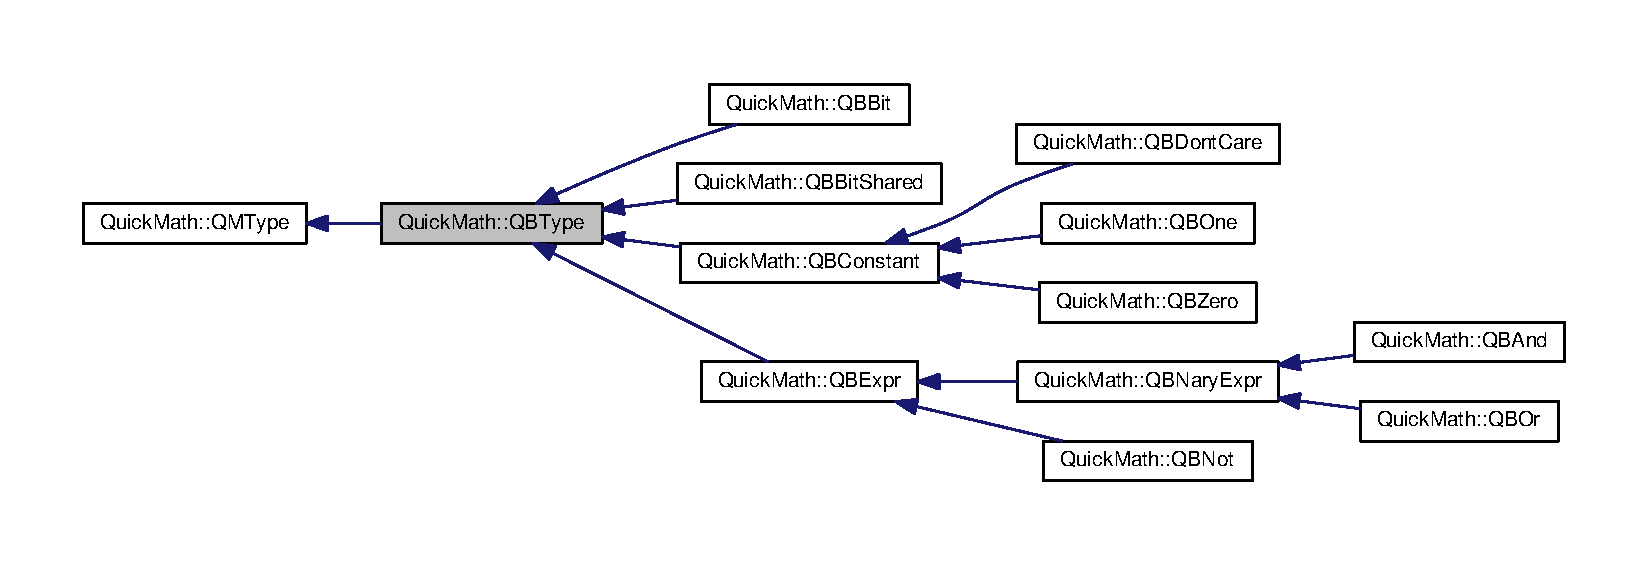
\includegraphics[width=350pt]{classQuickMath_1_1QBType__inherit__graph}
\end{center}
\end{figure}


Collaboration diagram for Quick\+Math\+:\+:Q\+B\+Type\+:
\nopagebreak
\begin{figure}[H]
\begin{center}
\leavevmode
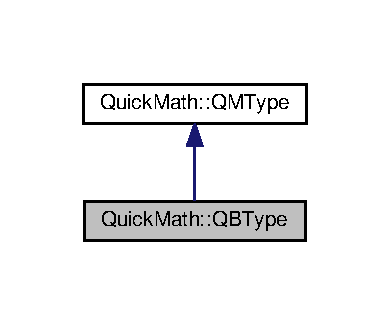
\includegraphics[width=187pt]{classQuickMath_1_1QBType__coll__graph}
\end{center}
\end{figure}
\subsection*{Public Member Functions}
\begin{DoxyCompactItemize}
\item 
virtual std\+::string \hyperlink{classQuickMath_1_1QBType_a12a08061a73649a9f79995469f8297d2}{to\+String} () const =0
\item 
virtual \hyperlink{namespaceQuickMath_aec13b08c42d9f8e688241623c8b379a0}{Q\+B\+Value} \hyperlink{classQuickMath_1_1QBType_a3fa2589c7d1fa4a52e79193bef845eeb}{value} () const =0
\item 
bool \hyperlink{classQuickMath_1_1QBType_a9d80f09c8d35de02d0cbb9317d1d326d}{is\+Bool\+Type} () const 
\item 
virtual bool \hyperlink{classQuickMath_1_1QBType_a0f612bd5695bf0e1cc56ebb98b18cf18}{is\+Var} () const 
\item 
virtual bool \hyperlink{classQuickMath_1_1QBType_a773a28a659747ec2a5c13d2a6f401404}{is\+Expr} () const 
\item 
virtual bool \hyperlink{classQuickMath_1_1QBType_a25cfa48db30dac38ace41b0997c089ab}{is\+And} () const 
\item 
virtual bool \hyperlink{classQuickMath_1_1QBType_a7c76be740f838beb84ea0b6b7c8cfeda}{is\+Or} () const 
\item 
virtual bool \hyperlink{classQuickMath_1_1QBType_a34cdcf8324b2091eae169992c1fcfa5b}{is\+Not} () const 
\item 
virtual bool \hyperlink{classQuickMath_1_1QBType_acf934f5d9bc0974db2ca1294b3d2f864}{is\+One} () const 
\item 
virtual bool \hyperlink{classQuickMath_1_1QBType_afcfd4750207efc2ac49bb87f45d315f3}{is\+Zero} () const 
\end{DoxyCompactItemize}


\subsection{Member Function Documentation}
\hypertarget{classQuickMath_1_1QBType_a25cfa48db30dac38ace41b0997c089ab}{}\index{Quick\+Math\+::\+Q\+B\+Type@{Quick\+Math\+::\+Q\+B\+Type}!is\+And@{is\+And}}
\index{is\+And@{is\+And}!Quick\+Math\+::\+Q\+B\+Type@{Quick\+Math\+::\+Q\+B\+Type}}
\subsubsection[{is\+And}]{\setlength{\rightskip}{0pt plus 5cm}virtual bool Quick\+Math\+::\+Q\+B\+Type\+::is\+And (
\begin{DoxyParamCaption}
{}
\end{DoxyParamCaption}
) const\hspace{0.3cm}{\ttfamily [inline]}, {\ttfamily [virtual]}}\label{classQuickMath_1_1QBType_a25cfa48db30dac38ace41b0997c089ab}


Reimplemented in \hyperlink{classQuickMath_1_1QBAnd_a9c722c8c7f3826faded75d70dd0f406c}{Quick\+Math\+::\+Q\+B\+And}, and \hyperlink{classQuickMath_1_1QBConstant_a750e108df9ba76a91a2e1096f01c5113}{Quick\+Math\+::\+Q\+B\+Constant}.

\hypertarget{classQuickMath_1_1QBType_a9d80f09c8d35de02d0cbb9317d1d326d}{}\index{Quick\+Math\+::\+Q\+B\+Type@{Quick\+Math\+::\+Q\+B\+Type}!is\+Bool\+Type@{is\+Bool\+Type}}
\index{is\+Bool\+Type@{is\+Bool\+Type}!Quick\+Math\+::\+Q\+B\+Type@{Quick\+Math\+::\+Q\+B\+Type}}
\subsubsection[{is\+Bool\+Type}]{\setlength{\rightskip}{0pt plus 5cm}bool Quick\+Math\+::\+Q\+B\+Type\+::is\+Bool\+Type (
\begin{DoxyParamCaption}
{}
\end{DoxyParamCaption}
) const\hspace{0.3cm}{\ttfamily [inline]}, {\ttfamily [virtual]}}\label{classQuickMath_1_1QBType_a9d80f09c8d35de02d0cbb9317d1d326d}


Reimplemented from \hyperlink{classQuickMath_1_1QMType_acb5baa3c93ea3cc6a25c358139b45dd5}{Quick\+Math\+::\+Q\+M\+Type}.

\hypertarget{classQuickMath_1_1QBType_a773a28a659747ec2a5c13d2a6f401404}{}\index{Quick\+Math\+::\+Q\+B\+Type@{Quick\+Math\+::\+Q\+B\+Type}!is\+Expr@{is\+Expr}}
\index{is\+Expr@{is\+Expr}!Quick\+Math\+::\+Q\+B\+Type@{Quick\+Math\+::\+Q\+B\+Type}}
\subsubsection[{is\+Expr}]{\setlength{\rightskip}{0pt plus 5cm}virtual bool Quick\+Math\+::\+Q\+B\+Type\+::is\+Expr (
\begin{DoxyParamCaption}
{}
\end{DoxyParamCaption}
) const\hspace{0.3cm}{\ttfamily [inline]}, {\ttfamily [virtual]}}\label{classQuickMath_1_1QBType_a773a28a659747ec2a5c13d2a6f401404}


Reimplemented in \hyperlink{classQuickMath_1_1QBExpr_a08e89c086e7cafce312c5766691a404a}{Quick\+Math\+::\+Q\+B\+Expr}, and \hyperlink{classQuickMath_1_1QBConstant_a6e7ee651a6a0436a16575064f401a941}{Quick\+Math\+::\+Q\+B\+Constant}.

\hypertarget{classQuickMath_1_1QBType_a34cdcf8324b2091eae169992c1fcfa5b}{}\index{Quick\+Math\+::\+Q\+B\+Type@{Quick\+Math\+::\+Q\+B\+Type}!is\+Not@{is\+Not}}
\index{is\+Not@{is\+Not}!Quick\+Math\+::\+Q\+B\+Type@{Quick\+Math\+::\+Q\+B\+Type}}
\subsubsection[{is\+Not}]{\setlength{\rightskip}{0pt plus 5cm}virtual bool Quick\+Math\+::\+Q\+B\+Type\+::is\+Not (
\begin{DoxyParamCaption}
{}
\end{DoxyParamCaption}
) const\hspace{0.3cm}{\ttfamily [inline]}, {\ttfamily [virtual]}}\label{classQuickMath_1_1QBType_a34cdcf8324b2091eae169992c1fcfa5b}


Reimplemented in \hyperlink{classQuickMath_1_1QBConstant_ae940dddd20874cec5c10b3fe6faf8bb2}{Quick\+Math\+::\+Q\+B\+Constant}, and \hyperlink{classQuickMath_1_1QBNot_ab39947bbca2904d4678eef80dae58145}{Quick\+Math\+::\+Q\+B\+Not}.

\hypertarget{classQuickMath_1_1QBType_acf934f5d9bc0974db2ca1294b3d2f864}{}\index{Quick\+Math\+::\+Q\+B\+Type@{Quick\+Math\+::\+Q\+B\+Type}!is\+One@{is\+One}}
\index{is\+One@{is\+One}!Quick\+Math\+::\+Q\+B\+Type@{Quick\+Math\+::\+Q\+B\+Type}}
\subsubsection[{is\+One}]{\setlength{\rightskip}{0pt plus 5cm}virtual bool Quick\+Math\+::\+Q\+B\+Type\+::is\+One (
\begin{DoxyParamCaption}
{}
\end{DoxyParamCaption}
) const\hspace{0.3cm}{\ttfamily [inline]}, {\ttfamily [virtual]}}\label{classQuickMath_1_1QBType_acf934f5d9bc0974db2ca1294b3d2f864}


Reimplemented in \hyperlink{classQuickMath_1_1QBOne_a2feb41d768849c7e1cc16a64898a2151}{Quick\+Math\+::\+Q\+B\+One}.

\hypertarget{classQuickMath_1_1QBType_a7c76be740f838beb84ea0b6b7c8cfeda}{}\index{Quick\+Math\+::\+Q\+B\+Type@{Quick\+Math\+::\+Q\+B\+Type}!is\+Or@{is\+Or}}
\index{is\+Or@{is\+Or}!Quick\+Math\+::\+Q\+B\+Type@{Quick\+Math\+::\+Q\+B\+Type}}
\subsubsection[{is\+Or}]{\setlength{\rightskip}{0pt plus 5cm}virtual bool Quick\+Math\+::\+Q\+B\+Type\+::is\+Or (
\begin{DoxyParamCaption}
{}
\end{DoxyParamCaption}
) const\hspace{0.3cm}{\ttfamily [inline]}, {\ttfamily [virtual]}}\label{classQuickMath_1_1QBType_a7c76be740f838beb84ea0b6b7c8cfeda}


Reimplemented in \hyperlink{classQuickMath_1_1QBConstant_ad9da48094fec1db5dbba35d362d56bf6}{Quick\+Math\+::\+Q\+B\+Constant}, and \hyperlink{classQuickMath_1_1QBOr_ab8f447a7b5fdcbde53cd69e79d4e552d}{Quick\+Math\+::\+Q\+B\+Or}.

\hypertarget{classQuickMath_1_1QBType_a0f612bd5695bf0e1cc56ebb98b18cf18}{}\index{Quick\+Math\+::\+Q\+B\+Type@{Quick\+Math\+::\+Q\+B\+Type}!is\+Var@{is\+Var}}
\index{is\+Var@{is\+Var}!Quick\+Math\+::\+Q\+B\+Type@{Quick\+Math\+::\+Q\+B\+Type}}
\subsubsection[{is\+Var}]{\setlength{\rightskip}{0pt plus 5cm}virtual bool Quick\+Math\+::\+Q\+B\+Type\+::is\+Var (
\begin{DoxyParamCaption}
{}
\end{DoxyParamCaption}
) const\hspace{0.3cm}{\ttfamily [inline]}, {\ttfamily [virtual]}}\label{classQuickMath_1_1QBType_a0f612bd5695bf0e1cc56ebb98b18cf18}


Reimplemented in \hyperlink{classQuickMath_1_1QBBit_a6f570086177786f5bf8191505f9216c1}{Quick\+Math\+::\+Q\+B\+Bit}, \hyperlink{classQuickMath_1_1QBBitShared_a69af2dec5fd73109c43f22c4230aa359}{Quick\+Math\+::\+Q\+B\+Bit\+Shared}, and \hyperlink{classQuickMath_1_1QBConstant_ac9ca2e6c87214135a275364956c66bae}{Quick\+Math\+::\+Q\+B\+Constant}.

\hypertarget{classQuickMath_1_1QBType_afcfd4750207efc2ac49bb87f45d315f3}{}\index{Quick\+Math\+::\+Q\+B\+Type@{Quick\+Math\+::\+Q\+B\+Type}!is\+Zero@{is\+Zero}}
\index{is\+Zero@{is\+Zero}!Quick\+Math\+::\+Q\+B\+Type@{Quick\+Math\+::\+Q\+B\+Type}}
\subsubsection[{is\+Zero}]{\setlength{\rightskip}{0pt plus 5cm}virtual bool Quick\+Math\+::\+Q\+B\+Type\+::is\+Zero (
\begin{DoxyParamCaption}
{}
\end{DoxyParamCaption}
) const\hspace{0.3cm}{\ttfamily [inline]}, {\ttfamily [virtual]}}\label{classQuickMath_1_1QBType_afcfd4750207efc2ac49bb87f45d315f3}


Reimplemented in \hyperlink{classQuickMath_1_1QBZero_afc6f5f8502d3f4eb19d1d2fe6dd5d1e4}{Quick\+Math\+::\+Q\+B\+Zero}.

\hypertarget{classQuickMath_1_1QBType_a12a08061a73649a9f79995469f8297d2}{}\index{Quick\+Math\+::\+Q\+B\+Type@{Quick\+Math\+::\+Q\+B\+Type}!to\+String@{to\+String}}
\index{to\+String@{to\+String}!Quick\+Math\+::\+Q\+B\+Type@{Quick\+Math\+::\+Q\+B\+Type}}
\subsubsection[{to\+String}]{\setlength{\rightskip}{0pt plus 5cm}virtual std\+::string Quick\+Math\+::\+Q\+B\+Type\+::to\+String (
\begin{DoxyParamCaption}
{}
\end{DoxyParamCaption}
) const\hspace{0.3cm}{\ttfamily [pure virtual]}}\label{classQuickMath_1_1QBType_a12a08061a73649a9f79995469f8297d2}


Implements \hyperlink{classQuickMath_1_1QMType_a031b83c87e4edae28c65adf8e268442b}{Quick\+Math\+::\+Q\+M\+Type}.



Implemented in \hyperlink{classQuickMath_1_1QBBit_acf69bfd78922571f1f0ac146c4eed56f}{Quick\+Math\+::\+Q\+B\+Bit}, \hyperlink{classQuickMath_1_1QBAnd_abf6c063e663077fdddc4aae96bfbca27}{Quick\+Math\+::\+Q\+B\+And}, \hyperlink{classQuickMath_1_1QBOr_ae835a7fda64bca20388ff3a869a9c928}{Quick\+Math\+::\+Q\+B\+Or}, \hyperlink{classQuickMath_1_1QBBitShared_ab1b3be4ae9548eac373e17038393f8a5}{Quick\+Math\+::\+Q\+B\+Bit\+Shared}, \hyperlink{classQuickMath_1_1QBConstant_a4e277add258b38b9f43da6dde48cd468}{Quick\+Math\+::\+Q\+B\+Constant}, and \hyperlink{classQuickMath_1_1QBNot_a946bcf1c86e2f59ea99537cb0fce2a80}{Quick\+Math\+::\+Q\+B\+Not}.

\hypertarget{classQuickMath_1_1QBType_a3fa2589c7d1fa4a52e79193bef845eeb}{}\index{Quick\+Math\+::\+Q\+B\+Type@{Quick\+Math\+::\+Q\+B\+Type}!value@{value}}
\index{value@{value}!Quick\+Math\+::\+Q\+B\+Type@{Quick\+Math\+::\+Q\+B\+Type}}
\subsubsection[{value}]{\setlength{\rightskip}{0pt plus 5cm}virtual {\bf Q\+B\+Value} Quick\+Math\+::\+Q\+B\+Type\+::value (
\begin{DoxyParamCaption}
{}
\end{DoxyParamCaption}
) const\hspace{0.3cm}{\ttfamily [pure virtual]}}\label{classQuickMath_1_1QBType_a3fa2589c7d1fa4a52e79193bef845eeb}


Implemented in \hyperlink{classQuickMath_1_1QBDontCare_a40a7cfa35c7e91d392493277d3e5078e}{Quick\+Math\+::\+Q\+B\+Dont\+Care}, \hyperlink{classQuickMath_1_1QBBit_add83657ec02a247eeb3883f8140d3223}{Quick\+Math\+::\+Q\+B\+Bit}, \hyperlink{classQuickMath_1_1QBZero_a1e7a0a5ca21ee665eccfc59ac7702403}{Quick\+Math\+::\+Q\+B\+Zero}, \hyperlink{classQuickMath_1_1QBOne_a2cc8ebd48be0d6edbfe0356d54d14919}{Quick\+Math\+::\+Q\+B\+One}, \hyperlink{classQuickMath_1_1QBAnd_abd8953fcd0d25729cec8c7d78355d217}{Quick\+Math\+::\+Q\+B\+And}, \hyperlink{classQuickMath_1_1QBOr_a385b6b29141e89e46629da29a8e38c8f}{Quick\+Math\+::\+Q\+B\+Or}, \hyperlink{classQuickMath_1_1QBBitShared_a27cbff4bed10a2e1f0f958f07d2f3485}{Quick\+Math\+::\+Q\+B\+Bit\+Shared}, \hyperlink{classQuickMath_1_1QBConstant_a399a700088d6327765b88652cea43c0e}{Quick\+Math\+::\+Q\+B\+Constant}, and \hyperlink{classQuickMath_1_1QBNot_a1b65e0c045a6ffb063a998b5751552d1}{Quick\+Math\+::\+Q\+B\+Not}.



The documentation for this class was generated from the following file\+:\begin{DoxyCompactItemize}
\item 
include/\+Q\+Bool/\hyperlink{QBType_8h}{Q\+B\+Type.\+h}\end{DoxyCompactItemize}

\hypertarget{classQuickMath_1_1QBVector}{}\section{Quick\+Math\+:\+:Q\+B\+Vector Class Reference}
\label{classQuickMath_1_1QBVector}\index{Quick\+Math\+::\+Q\+B\+Vector@{Quick\+Math\+::\+Q\+B\+Vector}}


{\ttfamily \#include $<$Q\+B\+Vector.\+h$>$}

\subsection*{Public Member Functions}
\begin{DoxyCompactItemize}
\item 
\hyperlink{classQuickMath_1_1QBVector_acc9096f5b85f712f8b6b135e0602cdc3}{Q\+B\+Vector} ()=default
\item 
\hyperlink{classQuickMath_1_1QBVector_a3127e531f0fa4359b9ef9e40b143feb6}{Q\+B\+Vector} (const std\+::vector$<$ \hyperlink{classQuickMath_1_1QBFunc}{Q\+B\+Func} $>$ \&\hyperlink{classQuickMath_1_1QBVector_a6e017544e097d563950754952fa42825}{bits})
\item 
\hyperlink{classQuickMath_1_1QBVector_a9bb76c4861cb54ab76f5cf11ffd3d7f5}{Q\+B\+Vector} (const std\+::vector$<$ \hyperlink{classQuickMath_1_1QBFunc}{Q\+B\+Func} $>$ \&\&\hyperlink{classQuickMath_1_1QBVector_a6e017544e097d563950754952fa42825}{bits})
\item 
\hyperlink{classQuickMath_1_1QBFunc}{Q\+B\+Func} \hyperlink{classQuickMath_1_1QBVector_a7ea835cb224b451dc0527007e668cf71}{operator\&} (const \hyperlink{classQuickMath_1_1QBVector}{Q\+B\+Vector} \&other) const 
\item 
\hyperlink{classQuickMath_1_1QBFunc}{Q\+B\+Func} \hyperlink{classQuickMath_1_1QBVector_ac5e95502680482c2f3b0bbe48f0563d6}{operator$\vert$} (const \hyperlink{classQuickMath_1_1QBVector}{Q\+B\+Vector} \&other) const 
\item 
\hyperlink{classQuickMath_1_1QBFunc}{Q\+B\+Func} \hyperlink{classQuickMath_1_1QBVector_a5246d8a7f9db8da8bc93c305bd1f7ca9}{operator$<$} (const \hyperlink{classQuickMath_1_1QBVector}{Q\+B\+Vector} \&other) const 
\item 
\hyperlink{classQuickMath_1_1QBFunc}{Q\+B\+Func} \hyperlink{classQuickMath_1_1QBVector_a6eecd7ac64f312a95fdfc18f0afdb9a9}{operator$<$=} (const \hyperlink{classQuickMath_1_1QBVector}{Q\+B\+Vector} \&other) const 
\item 
\hyperlink{classQuickMath_1_1QBFunc}{Q\+B\+Func} \hyperlink{classQuickMath_1_1QBVector_a112d9f6bdea9b694624521ec245dcae4}{operator$>$} (const \hyperlink{classQuickMath_1_1QBVector}{Q\+B\+Vector} \&other) const 
\item 
\hyperlink{classQuickMath_1_1QBFunc}{Q\+B\+Func} \hyperlink{classQuickMath_1_1QBVector_a553bbd02da9f430a1655a82ea1c230cc}{operator$>$=} (const \hyperlink{classQuickMath_1_1QBVector}{Q\+B\+Vector} \&other) const 
\item 
\hyperlink{classQuickMath_1_1QBFunc}{Q\+B\+Func} \hyperlink{classQuickMath_1_1QBVector_a57945ed39797ce903ca579524b50b2fd}{operator==} (const \hyperlink{classQuickMath_1_1QBVector}{Q\+B\+Vector} \&other) const 
\item 
\hyperlink{classQuickMath_1_1QBFunc}{Q\+B\+Func} \hyperlink{classQuickMath_1_1QBVector_a3b17560e6aa7f715274f9fb507c68007}{operator!=} (const \hyperlink{classQuickMath_1_1QBVector}{Q\+B\+Vector} \&other) const 
\item 
std\+::vector$<$ \hyperlink{classQuickMath_1_1QBFunc}{Q\+B\+Func} $>$\+::iterator \hyperlink{classQuickMath_1_1QBVector_aefa38c71c1d50322ffa9b5d9162b1054}{begin} ()
\item 
std\+::vector$<$ \hyperlink{classQuickMath_1_1QBFunc}{Q\+B\+Func} $>$\+::iterator \hyperlink{classQuickMath_1_1QBVector_ae92252e45c6fd308e28d85f554f5fb94}{end} ()
\item 
std\+::vector$<$ \hyperlink{classQuickMath_1_1QBFunc}{Q\+B\+Func} $>$\+::const\+\_\+iterator \hyperlink{classQuickMath_1_1QBVector_a79199571a7786d1ecb10122ddabbad8f}{begin} () const 
\item 
std\+::vector$<$ \hyperlink{classQuickMath_1_1QBFunc}{Q\+B\+Func} $>$\+::const\+\_\+iterator \hyperlink{classQuickMath_1_1QBVector_a2ca9b0a69061b150c1b6ce463f403481}{end} () const 
\item 
unsigned int \hyperlink{classQuickMath_1_1QBVector_a245af50766475e7d62c51c1e69b55caa}{size} () const 
\end{DoxyCompactItemize}
\subsection*{Private Attributes}
\begin{DoxyCompactItemize}
\item 
std\+::vector$<$ \hyperlink{classQuickMath_1_1QBFunc}{Q\+B\+Func} $>$ \hyperlink{classQuickMath_1_1QBVector_a6e017544e097d563950754952fa42825}{bits}
\end{DoxyCompactItemize}


\subsection{Constructor \& Destructor Documentation}
\hypertarget{classQuickMath_1_1QBVector_acc9096f5b85f712f8b6b135e0602cdc3}{}\index{Quick\+Math\+::\+Q\+B\+Vector@{Quick\+Math\+::\+Q\+B\+Vector}!Q\+B\+Vector@{Q\+B\+Vector}}
\index{Q\+B\+Vector@{Q\+B\+Vector}!Quick\+Math\+::\+Q\+B\+Vector@{Quick\+Math\+::\+Q\+B\+Vector}}
\subsubsection[{Q\+B\+Vector}]{\setlength{\rightskip}{0pt plus 5cm}Quick\+Math\+::\+Q\+B\+Vector\+::\+Q\+B\+Vector (
\begin{DoxyParamCaption}
{}
\end{DoxyParamCaption}
)\hspace{0.3cm}{\ttfamily [default]}}\label{classQuickMath_1_1QBVector_acc9096f5b85f712f8b6b135e0602cdc3}
\hypertarget{classQuickMath_1_1QBVector_a3127e531f0fa4359b9ef9e40b143feb6}{}\index{Quick\+Math\+::\+Q\+B\+Vector@{Quick\+Math\+::\+Q\+B\+Vector}!Q\+B\+Vector@{Q\+B\+Vector}}
\index{Q\+B\+Vector@{Q\+B\+Vector}!Quick\+Math\+::\+Q\+B\+Vector@{Quick\+Math\+::\+Q\+B\+Vector}}
\subsubsection[{Q\+B\+Vector}]{\setlength{\rightskip}{0pt plus 5cm}Quick\+Math\+::\+Q\+B\+Vector\+::\+Q\+B\+Vector (
\begin{DoxyParamCaption}
\item[{const std\+::vector$<$ {\bf Q\+B\+Func} $>$ \&}]{bits}
\end{DoxyParamCaption}
)}\label{classQuickMath_1_1QBVector_a3127e531f0fa4359b9ef9e40b143feb6}
\hypertarget{classQuickMath_1_1QBVector_a9bb76c4861cb54ab76f5cf11ffd3d7f5}{}\index{Quick\+Math\+::\+Q\+B\+Vector@{Quick\+Math\+::\+Q\+B\+Vector}!Q\+B\+Vector@{Q\+B\+Vector}}
\index{Q\+B\+Vector@{Q\+B\+Vector}!Quick\+Math\+::\+Q\+B\+Vector@{Quick\+Math\+::\+Q\+B\+Vector}}
\subsubsection[{Q\+B\+Vector}]{\setlength{\rightskip}{0pt plus 5cm}Quick\+Math\+::\+Q\+B\+Vector\+::\+Q\+B\+Vector (
\begin{DoxyParamCaption}
\item[{const std\+::vector$<$ {\bf Q\+B\+Func} $>$ \&\&}]{bits}
\end{DoxyParamCaption}
)}\label{classQuickMath_1_1QBVector_a9bb76c4861cb54ab76f5cf11ffd3d7f5}


\subsection{Member Function Documentation}
\hypertarget{classQuickMath_1_1QBVector_aefa38c71c1d50322ffa9b5d9162b1054}{}\index{Quick\+Math\+::\+Q\+B\+Vector@{Quick\+Math\+::\+Q\+B\+Vector}!begin@{begin}}
\index{begin@{begin}!Quick\+Math\+::\+Q\+B\+Vector@{Quick\+Math\+::\+Q\+B\+Vector}}
\subsubsection[{begin}]{\setlength{\rightskip}{0pt plus 5cm}std\+::vector$<$ {\bf Q\+B\+Func} $>$\+::iterator Quick\+Math\+::\+Q\+B\+Vector\+::begin (
\begin{DoxyParamCaption}
{}
\end{DoxyParamCaption}
)}\label{classQuickMath_1_1QBVector_aefa38c71c1d50322ffa9b5d9162b1054}
\hypertarget{classQuickMath_1_1QBVector_a79199571a7786d1ecb10122ddabbad8f}{}\index{Quick\+Math\+::\+Q\+B\+Vector@{Quick\+Math\+::\+Q\+B\+Vector}!begin@{begin}}
\index{begin@{begin}!Quick\+Math\+::\+Q\+B\+Vector@{Quick\+Math\+::\+Q\+B\+Vector}}
\subsubsection[{begin}]{\setlength{\rightskip}{0pt plus 5cm}std\+::vector$<$ {\bf Q\+B\+Func} $>$\+::const\+\_\+iterator Quick\+Math\+::\+Q\+B\+Vector\+::begin (
\begin{DoxyParamCaption}
{}
\end{DoxyParamCaption}
) const}\label{classQuickMath_1_1QBVector_a79199571a7786d1ecb10122ddabbad8f}
\hypertarget{classQuickMath_1_1QBVector_ae92252e45c6fd308e28d85f554f5fb94}{}\index{Quick\+Math\+::\+Q\+B\+Vector@{Quick\+Math\+::\+Q\+B\+Vector}!end@{end}}
\index{end@{end}!Quick\+Math\+::\+Q\+B\+Vector@{Quick\+Math\+::\+Q\+B\+Vector}}
\subsubsection[{end}]{\setlength{\rightskip}{0pt plus 5cm}std\+::vector$<$ {\bf Q\+B\+Func} $>$\+::iterator Quick\+Math\+::\+Q\+B\+Vector\+::end (
\begin{DoxyParamCaption}
{}
\end{DoxyParamCaption}
)}\label{classQuickMath_1_1QBVector_ae92252e45c6fd308e28d85f554f5fb94}
\hypertarget{classQuickMath_1_1QBVector_a2ca9b0a69061b150c1b6ce463f403481}{}\index{Quick\+Math\+::\+Q\+B\+Vector@{Quick\+Math\+::\+Q\+B\+Vector}!end@{end}}
\index{end@{end}!Quick\+Math\+::\+Q\+B\+Vector@{Quick\+Math\+::\+Q\+B\+Vector}}
\subsubsection[{end}]{\setlength{\rightskip}{0pt plus 5cm}std\+::vector$<$ {\bf Q\+B\+Func} $>$\+::const\+\_\+iterator Quick\+Math\+::\+Q\+B\+Vector\+::end (
\begin{DoxyParamCaption}
{}
\end{DoxyParamCaption}
) const}\label{classQuickMath_1_1QBVector_a2ca9b0a69061b150c1b6ce463f403481}
\hypertarget{classQuickMath_1_1QBVector_a3b17560e6aa7f715274f9fb507c68007}{}\index{Quick\+Math\+::\+Q\+B\+Vector@{Quick\+Math\+::\+Q\+B\+Vector}!operator"!=@{operator"!=}}
\index{operator"!=@{operator"!=}!Quick\+Math\+::\+Q\+B\+Vector@{Quick\+Math\+::\+Q\+B\+Vector}}
\subsubsection[{operator"!=}]{\setlength{\rightskip}{0pt plus 5cm}{\bf Q\+B\+Func} Quick\+Math\+::\+Q\+B\+Vector\+::operator!= (
\begin{DoxyParamCaption}
\item[{const {\bf Q\+B\+Vector} \&}]{other}
\end{DoxyParamCaption}
) const}\label{classQuickMath_1_1QBVector_a3b17560e6aa7f715274f9fb507c68007}
\hypertarget{classQuickMath_1_1QBVector_a7ea835cb224b451dc0527007e668cf71}{}\index{Quick\+Math\+::\+Q\+B\+Vector@{Quick\+Math\+::\+Q\+B\+Vector}!operator\&@{operator\&}}
\index{operator\&@{operator\&}!Quick\+Math\+::\+Q\+B\+Vector@{Quick\+Math\+::\+Q\+B\+Vector}}
\subsubsection[{operator\&}]{\setlength{\rightskip}{0pt plus 5cm}{\bf Q\+B\+Func} Quick\+Math\+::\+Q\+B\+Vector\+::operator\& (
\begin{DoxyParamCaption}
\item[{const {\bf Q\+B\+Vector} \&}]{other}
\end{DoxyParamCaption}
) const}\label{classQuickMath_1_1QBVector_a7ea835cb224b451dc0527007e668cf71}
\hypertarget{classQuickMath_1_1QBVector_a5246d8a7f9db8da8bc93c305bd1f7ca9}{}\index{Quick\+Math\+::\+Q\+B\+Vector@{Quick\+Math\+::\+Q\+B\+Vector}!operator$<$@{operator$<$}}
\index{operator$<$@{operator$<$}!Quick\+Math\+::\+Q\+B\+Vector@{Quick\+Math\+::\+Q\+B\+Vector}}
\subsubsection[{operator$<$}]{\setlength{\rightskip}{0pt plus 5cm}{\bf Q\+B\+Func} Quick\+Math\+::\+Q\+B\+Vector\+::operator$<$ (
\begin{DoxyParamCaption}
\item[{const {\bf Q\+B\+Vector} \&}]{other}
\end{DoxyParamCaption}
) const}\label{classQuickMath_1_1QBVector_a5246d8a7f9db8da8bc93c305bd1f7ca9}
\hypertarget{classQuickMath_1_1QBVector_a6eecd7ac64f312a95fdfc18f0afdb9a9}{}\index{Quick\+Math\+::\+Q\+B\+Vector@{Quick\+Math\+::\+Q\+B\+Vector}!operator$<$=@{operator$<$=}}
\index{operator$<$=@{operator$<$=}!Quick\+Math\+::\+Q\+B\+Vector@{Quick\+Math\+::\+Q\+B\+Vector}}
\subsubsection[{operator$<$=}]{\setlength{\rightskip}{0pt plus 5cm}{\bf Q\+B\+Func} Quick\+Math\+::\+Q\+B\+Vector\+::operator$<$= (
\begin{DoxyParamCaption}
\item[{const {\bf Q\+B\+Vector} \&}]{other}
\end{DoxyParamCaption}
) const}\label{classQuickMath_1_1QBVector_a6eecd7ac64f312a95fdfc18f0afdb9a9}
\hypertarget{classQuickMath_1_1QBVector_a57945ed39797ce903ca579524b50b2fd}{}\index{Quick\+Math\+::\+Q\+B\+Vector@{Quick\+Math\+::\+Q\+B\+Vector}!operator==@{operator==}}
\index{operator==@{operator==}!Quick\+Math\+::\+Q\+B\+Vector@{Quick\+Math\+::\+Q\+B\+Vector}}
\subsubsection[{operator==}]{\setlength{\rightskip}{0pt plus 5cm}{\bf Q\+B\+Func} Quick\+Math\+::\+Q\+B\+Vector\+::operator== (
\begin{DoxyParamCaption}
\item[{const {\bf Q\+B\+Vector} \&}]{other}
\end{DoxyParamCaption}
) const}\label{classQuickMath_1_1QBVector_a57945ed39797ce903ca579524b50b2fd}
\hypertarget{classQuickMath_1_1QBVector_a112d9f6bdea9b694624521ec245dcae4}{}\index{Quick\+Math\+::\+Q\+B\+Vector@{Quick\+Math\+::\+Q\+B\+Vector}!operator$>$@{operator$>$}}
\index{operator$>$@{operator$>$}!Quick\+Math\+::\+Q\+B\+Vector@{Quick\+Math\+::\+Q\+B\+Vector}}
\subsubsection[{operator$>$}]{\setlength{\rightskip}{0pt plus 5cm}{\bf Q\+B\+Func} Quick\+Math\+::\+Q\+B\+Vector\+::operator$>$ (
\begin{DoxyParamCaption}
\item[{const {\bf Q\+B\+Vector} \&}]{other}
\end{DoxyParamCaption}
) const}\label{classQuickMath_1_1QBVector_a112d9f6bdea9b694624521ec245dcae4}
\hypertarget{classQuickMath_1_1QBVector_a553bbd02da9f430a1655a82ea1c230cc}{}\index{Quick\+Math\+::\+Q\+B\+Vector@{Quick\+Math\+::\+Q\+B\+Vector}!operator$>$=@{operator$>$=}}
\index{operator$>$=@{operator$>$=}!Quick\+Math\+::\+Q\+B\+Vector@{Quick\+Math\+::\+Q\+B\+Vector}}
\subsubsection[{operator$>$=}]{\setlength{\rightskip}{0pt plus 5cm}{\bf Q\+B\+Func} Quick\+Math\+::\+Q\+B\+Vector\+::operator$>$= (
\begin{DoxyParamCaption}
\item[{const {\bf Q\+B\+Vector} \&}]{other}
\end{DoxyParamCaption}
) const}\label{classQuickMath_1_1QBVector_a553bbd02da9f430a1655a82ea1c230cc}
\hypertarget{classQuickMath_1_1QBVector_ac5e95502680482c2f3b0bbe48f0563d6}{}\index{Quick\+Math\+::\+Q\+B\+Vector@{Quick\+Math\+::\+Q\+B\+Vector}!operator\texttt{"|}@{operator\texttt{"|}}}
\index{operator\texttt{"|}@{operator\texttt{"|}}!Quick\+Math\+::\+Q\+B\+Vector@{Quick\+Math\+::\+Q\+B\+Vector}}
\subsubsection[{operator\texttt{"|}}]{\setlength{\rightskip}{0pt plus 5cm}{\bf Q\+B\+Func} Quick\+Math\+::\+Q\+B\+Vector\+::operator$\vert$ (
\begin{DoxyParamCaption}
\item[{const {\bf Q\+B\+Vector} \&}]{other}
\end{DoxyParamCaption}
) const}\label{classQuickMath_1_1QBVector_ac5e95502680482c2f3b0bbe48f0563d6}
\hypertarget{classQuickMath_1_1QBVector_a245af50766475e7d62c51c1e69b55caa}{}\index{Quick\+Math\+::\+Q\+B\+Vector@{Quick\+Math\+::\+Q\+B\+Vector}!size@{size}}
\index{size@{size}!Quick\+Math\+::\+Q\+B\+Vector@{Quick\+Math\+::\+Q\+B\+Vector}}
\subsubsection[{size}]{\setlength{\rightskip}{0pt plus 5cm}unsigned int Quick\+Math\+::\+Q\+B\+Vector\+::size (
\begin{DoxyParamCaption}
{}
\end{DoxyParamCaption}
) const}\label{classQuickMath_1_1QBVector_a245af50766475e7d62c51c1e69b55caa}


\subsection{Member Data Documentation}
\hypertarget{classQuickMath_1_1QBVector_a6e017544e097d563950754952fa42825}{}\index{Quick\+Math\+::\+Q\+B\+Vector@{Quick\+Math\+::\+Q\+B\+Vector}!bits@{bits}}
\index{bits@{bits}!Quick\+Math\+::\+Q\+B\+Vector@{Quick\+Math\+::\+Q\+B\+Vector}}
\subsubsection[{bits}]{\setlength{\rightskip}{0pt plus 5cm}std\+::vector$<${\bf Q\+B\+Func}$>$ Quick\+Math\+::\+Q\+B\+Vector\+::bits\hspace{0.3cm}{\ttfamily [private]}}\label{classQuickMath_1_1QBVector_a6e017544e097d563950754952fa42825}


The documentation for this class was generated from the following files\+:\begin{DoxyCompactItemize}
\item 
include/\+Q\+Bool/\hyperlink{QBVector_8h}{Q\+B\+Vector.\+h}\item 
src/\+Q\+Bool/\hyperlink{QBVector_8cpp}{Q\+B\+Vector.\+cpp}\end{DoxyCompactItemize}

\hypertarget{classQuickMath_1_1QBZero}{}\section{Quick\+Math\+:\+:Q\+B\+Zero Class Reference}
\label{classQuickMath_1_1QBZero}\index{Quick\+Math\+::\+Q\+B\+Zero@{Quick\+Math\+::\+Q\+B\+Zero}}


{\ttfamily \#include $<$Q\+B\+Constants.\+h$>$}



Inheritance diagram for Quick\+Math\+:\+:Q\+B\+Zero\+:
\nopagebreak
\begin{figure}[H]
\begin{center}
\leavevmode
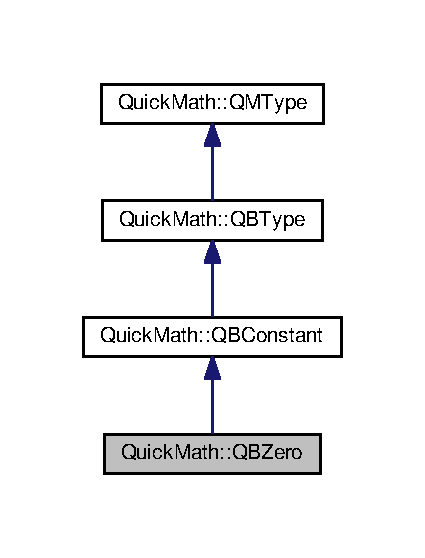
\includegraphics[width=204pt]{classQuickMath_1_1QBZero__inherit__graph}
\end{center}
\end{figure}


Collaboration diagram for Quick\+Math\+:\+:Q\+B\+Zero\+:
\nopagebreak
\begin{figure}[H]
\begin{center}
\leavevmode
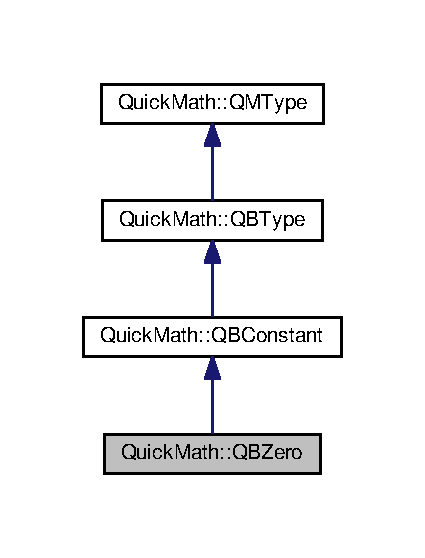
\includegraphics[width=204pt]{classQuickMath_1_1QBZero__coll__graph}
\end{center}
\end{figure}
\subsection*{Public Member Functions}
\begin{DoxyCompactItemize}
\item 
\hyperlink{namespaceQuickMath_aec13b08c42d9f8e688241623c8b379a0}{Q\+B\+Value} \hyperlink{classQuickMath_1_1QBZero_a1e7a0a5ca21ee665eccfc59ac7702403}{value} () const 
\item 
std\+::unique\+\_\+ptr$<$ \hyperlink{classQuickMath_1_1QMType}{Q\+M\+Type} $>$ \hyperlink{classQuickMath_1_1QBZero_ab2bff50f0df2163ffff4cc07d207df1e}{clone} () const 
\item 
bool \hyperlink{classQuickMath_1_1QBZero_afc6f5f8502d3f4eb19d1d2fe6dd5d1e4}{is\+Zero} () const 
\end{DoxyCompactItemize}


\subsection{Member Function Documentation}
\hypertarget{classQuickMath_1_1QBZero_ab2bff50f0df2163ffff4cc07d207df1e}{}\index{Quick\+Math\+::\+Q\+B\+Zero@{Quick\+Math\+::\+Q\+B\+Zero}!clone@{clone}}
\index{clone@{clone}!Quick\+Math\+::\+Q\+B\+Zero@{Quick\+Math\+::\+Q\+B\+Zero}}
\subsubsection[{clone}]{\setlength{\rightskip}{0pt plus 5cm}std\+::unique\+\_\+ptr$<$ {\bf Q\+M\+Type} $>$ Quick\+Math\+::\+Q\+B\+Zero\+::clone (
\begin{DoxyParamCaption}
{}
\end{DoxyParamCaption}
) const\hspace{0.3cm}{\ttfamily [virtual]}}\label{classQuickMath_1_1QBZero_ab2bff50f0df2163ffff4cc07d207df1e}


Implements \hyperlink{classQuickMath_1_1QMType_a15b2a74a662417da99c6da9b7aaeff77}{Quick\+Math\+::\+Q\+M\+Type}.

\hypertarget{classQuickMath_1_1QBZero_afc6f5f8502d3f4eb19d1d2fe6dd5d1e4}{}\index{Quick\+Math\+::\+Q\+B\+Zero@{Quick\+Math\+::\+Q\+B\+Zero}!is\+Zero@{is\+Zero}}
\index{is\+Zero@{is\+Zero}!Quick\+Math\+::\+Q\+B\+Zero@{Quick\+Math\+::\+Q\+B\+Zero}}
\subsubsection[{is\+Zero}]{\setlength{\rightskip}{0pt plus 5cm}bool Quick\+Math\+::\+Q\+B\+Zero\+::is\+Zero (
\begin{DoxyParamCaption}
{}
\end{DoxyParamCaption}
) const\hspace{0.3cm}{\ttfamily [virtual]}}\label{classQuickMath_1_1QBZero_afc6f5f8502d3f4eb19d1d2fe6dd5d1e4}


Reimplemented from \hyperlink{classQuickMath_1_1QBType_afcfd4750207efc2ac49bb87f45d315f3}{Quick\+Math\+::\+Q\+B\+Type}.

\hypertarget{classQuickMath_1_1QBZero_a1e7a0a5ca21ee665eccfc59ac7702403}{}\index{Quick\+Math\+::\+Q\+B\+Zero@{Quick\+Math\+::\+Q\+B\+Zero}!value@{value}}
\index{value@{value}!Quick\+Math\+::\+Q\+B\+Zero@{Quick\+Math\+::\+Q\+B\+Zero}}
\subsubsection[{value}]{\setlength{\rightskip}{0pt plus 5cm}{\bf Q\+B\+Value} Quick\+Math\+::\+Q\+B\+Zero\+::value (
\begin{DoxyParamCaption}
{}
\end{DoxyParamCaption}
) const\hspace{0.3cm}{\ttfamily [virtual]}}\label{classQuickMath_1_1QBZero_a1e7a0a5ca21ee665eccfc59ac7702403}


Implements \hyperlink{classQuickMath_1_1QBConstant_a399a700088d6327765b88652cea43c0e}{Quick\+Math\+::\+Q\+B\+Constant}.



The documentation for this class was generated from the following files\+:\begin{DoxyCompactItemize}
\item 
include/\+Q\+Bool/\hyperlink{QBConstants_8h}{Q\+B\+Constants.\+h}\item 
src/\+Q\+Bool/\hyperlink{QBConstants_8cpp}{Q\+B\+Constants.\+cpp}\end{DoxyCompactItemize}

\hypertarget{classQuickMath_1_1QExpr}{}\section{Quick\+Math\+:\+:Q\+Expr Class Reference}
\label{classQuickMath_1_1QExpr}\index{Quick\+Math\+::\+Q\+Expr@{Quick\+Math\+::\+Q\+Expr}}


{\ttfamily \#include $<$Q\+Expr.\+h$>$}



Inheritance diagram for Quick\+Math\+:\+:Q\+Expr\+:
\nopagebreak
\begin{figure}[H]
\begin{center}
\leavevmode
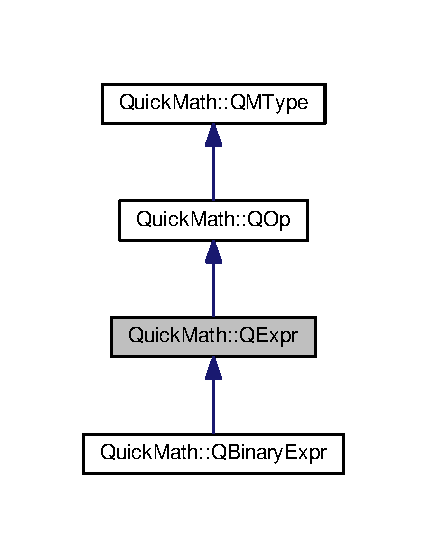
\includegraphics[width=205pt]{classQuickMath_1_1QExpr__inherit__graph}
\end{center}
\end{figure}


Collaboration diagram for Quick\+Math\+:\+:Q\+Expr\+:
\nopagebreak
\begin{figure}[H]
\begin{center}
\leavevmode
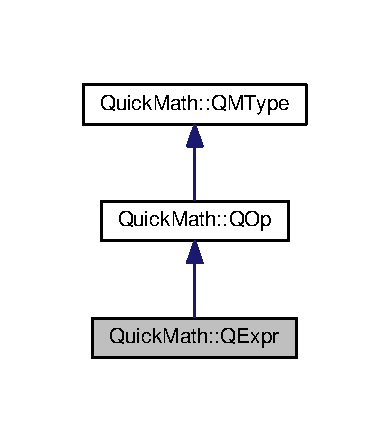
\includegraphics[width=187pt]{classQuickMath_1_1QExpr__coll__graph}
\end{center}
\end{figure}
\subsection*{Public Member Functions}
\begin{DoxyCompactItemize}
\item 
bool \hyperlink{classQuickMath_1_1QExpr_a405e53844f259aae5d4cc989afd0eb70}{is\+Expr} () const 
\item 
virtual \hyperlink{namespaceQuickMath_a0a6c67b9dab0cfd5f3e711b0573545cb}{Q\+M\+Op\+Type} \hyperlink{classQuickMath_1_1QExpr_aa58e1151560eff36439d1a55562c07d7}{op\+Type} () const 
\end{DoxyCompactItemize}
\subsection*{Protected Attributes}
\begin{DoxyCompactItemize}
\item 
\hyperlink{namespaceQuickMath_a0a6c67b9dab0cfd5f3e711b0573545cb}{Q\+M\+Op\+Type} \hyperlink{classQuickMath_1_1QExpr_adb14b90658bcec8024881371b9b87c10}{op}
\end{DoxyCompactItemize}


\subsection{Member Function Documentation}
\hypertarget{classQuickMath_1_1QExpr_a405e53844f259aae5d4cc989afd0eb70}{}\index{Quick\+Math\+::\+Q\+Expr@{Quick\+Math\+::\+Q\+Expr}!is\+Expr@{is\+Expr}}
\index{is\+Expr@{is\+Expr}!Quick\+Math\+::\+Q\+Expr@{Quick\+Math\+::\+Q\+Expr}}
\subsubsection[{is\+Expr}]{\setlength{\rightskip}{0pt plus 5cm}bool Quick\+Math\+::\+Q\+Expr\+::is\+Expr (
\begin{DoxyParamCaption}
{}
\end{DoxyParamCaption}
) const}\label{classQuickMath_1_1QExpr_a405e53844f259aae5d4cc989afd0eb70}
\hypertarget{classQuickMath_1_1QExpr_aa58e1151560eff36439d1a55562c07d7}{}\index{Quick\+Math\+::\+Q\+Expr@{Quick\+Math\+::\+Q\+Expr}!op\+Type@{op\+Type}}
\index{op\+Type@{op\+Type}!Quick\+Math\+::\+Q\+Expr@{Quick\+Math\+::\+Q\+Expr}}
\subsubsection[{op\+Type}]{\setlength{\rightskip}{0pt plus 5cm}{\bf Q\+M\+Op\+Type} Quick\+Math\+::\+Q\+Expr\+::op\+Type (
\begin{DoxyParamCaption}
{}
\end{DoxyParamCaption}
) const\hspace{0.3cm}{\ttfamily [virtual]}}\label{classQuickMath_1_1QExpr_aa58e1151560eff36439d1a55562c07d7}


\subsection{Member Data Documentation}
\hypertarget{classQuickMath_1_1QExpr_adb14b90658bcec8024881371b9b87c10}{}\index{Quick\+Math\+::\+Q\+Expr@{Quick\+Math\+::\+Q\+Expr}!op@{op}}
\index{op@{op}!Quick\+Math\+::\+Q\+Expr@{Quick\+Math\+::\+Q\+Expr}}
\subsubsection[{op}]{\setlength{\rightskip}{0pt plus 5cm}{\bf Q\+M\+Op\+Type} Quick\+Math\+::\+Q\+Expr\+::op\hspace{0.3cm}{\ttfamily [protected]}}\label{classQuickMath_1_1QExpr_adb14b90658bcec8024881371b9b87c10}


The documentation for this class was generated from the following files\+:\begin{DoxyCompactItemize}
\item 
include/\+Q\+Mix/\hyperlink{QExpr_8h}{Q\+Expr.\+h}\item 
src/\+Q\+Mix/\hyperlink{QExpr_8cpp}{Q\+Expr.\+cpp}\end{DoxyCompactItemize}

\hypertarget{classQuickMath_1_1QFBinaryExpr}{}\section{Quick\+Math\+:\+:Q\+F\+Binary\+Expr Class Reference}
\label{classQuickMath_1_1QFBinaryExpr}\index{Quick\+Math\+::\+Q\+F\+Binary\+Expr@{Quick\+Math\+::\+Q\+F\+Binary\+Expr}}


{\ttfamily \#include $<$Q\+F\+Binary\+Expr.\+h$>$}



Inheritance diagram for Quick\+Math\+:\+:Q\+F\+Binary\+Expr\+:
\nopagebreak
\begin{figure}[H]
\begin{center}
\leavevmode
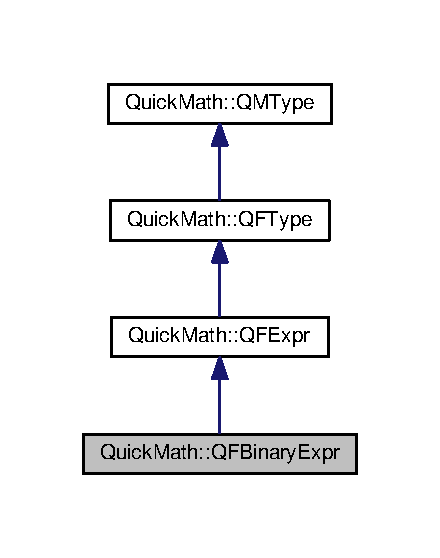
\includegraphics[width=211pt]{classQuickMath_1_1QFBinaryExpr__inherit__graph}
\end{center}
\end{figure}


Collaboration diagram for Quick\+Math\+:\+:Q\+F\+Binary\+Expr\+:
\nopagebreak
\begin{figure}[H]
\begin{center}
\leavevmode
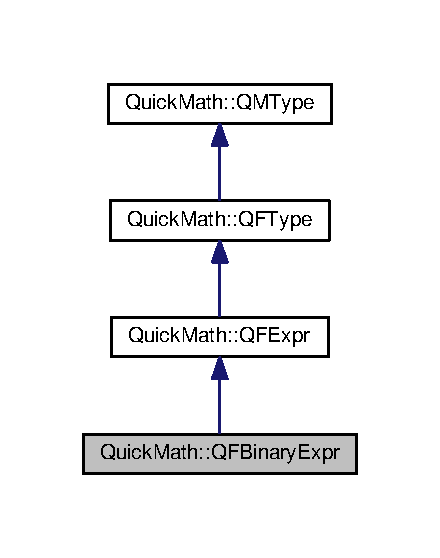
\includegraphics[width=211pt]{classQuickMath_1_1QFBinaryExpr__coll__graph}
\end{center}
\end{figure}
\subsection*{Public Member Functions}
\begin{DoxyCompactItemize}
\item 
\hyperlink{classQuickMath_1_1QFBinaryExpr_ae6ec6206deb318cf4b2865c879aa9fc6}{Q\+F\+Binary\+Expr} ()=default
\item 
\hyperlink{classQuickMath_1_1QFBinaryExpr_af88afa909437217a78f67c8cf617e244}{Q\+F\+Binary\+Expr} (const \hyperlink{classQuickMath_1_1QFBinaryExpr}{Q\+F\+Binary\+Expr} \&other)
\item 
\hyperlink{classQuickMath_1_1QFBinaryExpr_a61d5fbfee98a7795dc1837db4482cc76}{Q\+F\+Binary\+Expr} (\hyperlink{namespaceQuickMath_a0a6c67b9dab0cfd5f3e711b0573545cb}{Q\+M\+Op\+Type} type, std\+::unique\+\_\+ptr$<$ \hyperlink{classQuickMath_1_1QFType}{Q\+F\+Type} $>$ a, std\+::unique\+\_\+ptr$<$ \hyperlink{classQuickMath_1_1QFType}{Q\+F\+Type} $>$ b)
\item 
\hyperlink{classQuickMath_1_1QFBinaryExpr_a8bff2704629a1ccc2050933709ce21b5}{Q\+F\+Binary\+Expr} (\hyperlink{namespaceQuickMath_a0a6c67b9dab0cfd5f3e711b0573545cb}{Q\+M\+Op\+Type} type, const \hyperlink{classQuickMath_1_1QFType}{Q\+F\+Type} \&a, const \hyperlink{classQuickMath_1_1QFType}{Q\+F\+Type} \&b)
\item 
\hyperlink{classQuickMath_1_1QFBinaryExpr}{Q\+F\+Binary\+Expr} \& \hyperlink{classQuickMath_1_1QFBinaryExpr_a2bda8f3570dc2b9e926d0b6efe9efcfd}{operator=} (const \hyperlink{classQuickMath_1_1QFBinaryExpr}{Q\+F\+Binary\+Expr} \&other)
\item 
\hyperlink{classQuickMath_1_1QFBinaryExpr}{Q\+F\+Binary\+Expr} \& \hyperlink{classQuickMath_1_1QFBinaryExpr_a615303d5a9e584de83ae489578aefe04}{operator=} (\hyperlink{classQuickMath_1_1QFBinaryExpr}{Q\+F\+Binary\+Expr} \&\&other)
\item 
std\+::string \hyperlink{classQuickMath_1_1QFBinaryExpr_a676c949b30d14f919dcdf20151a5b3fe}{to\+String} () const 
\item 
const \hyperlink{classQuickMath_1_1QFType}{Q\+F\+Type} $\ast$ \hyperlink{classQuickMath_1_1QFBinaryExpr_a1b68ff06a8386d1c1f95a1a781660d98}{left\+Operand} () const 
\item 
const \hyperlink{classQuickMath_1_1QFType}{Q\+F\+Type} $\ast$ \hyperlink{classQuickMath_1_1QFBinaryExpr_aead11f57ff726fba3e6227d567737bf9}{right\+Operand} () const 
\item 
virtual std\+::array$<$ std\+::unique\+\_\+ptr$<$ \hyperlink{classQuickMath_1_1QFType}{Q\+F\+Type} $>$, 2 $>$\+::const\+\_\+iterator \hyperlink{classQuickMath_1_1QFBinaryExpr_a0f9c25472343592ffbd3337da671a25a}{begin} () const 
\item 
virtual std\+::array$<$ std\+::unique\+\_\+ptr$<$ \hyperlink{classQuickMath_1_1QFType}{Q\+F\+Type} $>$, 2 $>$\+::const\+\_\+iterator \hyperlink{classQuickMath_1_1QFBinaryExpr_ad22a3e71d2f7170528a499c994439a7b}{end} () const 
\item 
virtual std\+::unique\+\_\+ptr$<$ \hyperlink{classQuickMath_1_1QMType}{Q\+M\+Type} $>$ \hyperlink{classQuickMath_1_1QFBinaryExpr_a7f49aef7dd9b8b4c144bbf30395d9051}{clone} () const 
\end{DoxyCompactItemize}
\subsection*{Protected Attributes}
\begin{DoxyCompactItemize}
\item 
std\+::array$<$ std\+::unique\+\_\+ptr$<$ \hyperlink{classQuickMath_1_1QFType}{Q\+F\+Type} $>$, 2 $>$ \hyperlink{classQuickMath_1_1QFBinaryExpr_a9cf52ed63874809fd4244c5ff5ac441d}{operands}
\end{DoxyCompactItemize}


\subsection{Constructor \& Destructor Documentation}
\hypertarget{classQuickMath_1_1QFBinaryExpr_ae6ec6206deb318cf4b2865c879aa9fc6}{}\index{Quick\+Math\+::\+Q\+F\+Binary\+Expr@{Quick\+Math\+::\+Q\+F\+Binary\+Expr}!Q\+F\+Binary\+Expr@{Q\+F\+Binary\+Expr}}
\index{Q\+F\+Binary\+Expr@{Q\+F\+Binary\+Expr}!Quick\+Math\+::\+Q\+F\+Binary\+Expr@{Quick\+Math\+::\+Q\+F\+Binary\+Expr}}
\subsubsection[{Q\+F\+Binary\+Expr}]{\setlength{\rightskip}{0pt plus 5cm}Quick\+Math\+::\+Q\+F\+Binary\+Expr\+::\+Q\+F\+Binary\+Expr (
\begin{DoxyParamCaption}
{}
\end{DoxyParamCaption}
)\hspace{0.3cm}{\ttfamily [default]}}\label{classQuickMath_1_1QFBinaryExpr_ae6ec6206deb318cf4b2865c879aa9fc6}
\hypertarget{classQuickMath_1_1QFBinaryExpr_af88afa909437217a78f67c8cf617e244}{}\index{Quick\+Math\+::\+Q\+F\+Binary\+Expr@{Quick\+Math\+::\+Q\+F\+Binary\+Expr}!Q\+F\+Binary\+Expr@{Q\+F\+Binary\+Expr}}
\index{Q\+F\+Binary\+Expr@{Q\+F\+Binary\+Expr}!Quick\+Math\+::\+Q\+F\+Binary\+Expr@{Quick\+Math\+::\+Q\+F\+Binary\+Expr}}
\subsubsection[{Q\+F\+Binary\+Expr}]{\setlength{\rightskip}{0pt plus 5cm}Quick\+Math\+::\+Q\+F\+Binary\+Expr\+::\+Q\+F\+Binary\+Expr (
\begin{DoxyParamCaption}
\item[{const {\bf Q\+F\+Binary\+Expr} \&}]{other}
\end{DoxyParamCaption}
)}\label{classQuickMath_1_1QFBinaryExpr_af88afa909437217a78f67c8cf617e244}
\hypertarget{classQuickMath_1_1QFBinaryExpr_a61d5fbfee98a7795dc1837db4482cc76}{}\index{Quick\+Math\+::\+Q\+F\+Binary\+Expr@{Quick\+Math\+::\+Q\+F\+Binary\+Expr}!Q\+F\+Binary\+Expr@{Q\+F\+Binary\+Expr}}
\index{Q\+F\+Binary\+Expr@{Q\+F\+Binary\+Expr}!Quick\+Math\+::\+Q\+F\+Binary\+Expr@{Quick\+Math\+::\+Q\+F\+Binary\+Expr}}
\subsubsection[{Q\+F\+Binary\+Expr}]{\setlength{\rightskip}{0pt plus 5cm}Quick\+Math\+::\+Q\+F\+Binary\+Expr\+::\+Q\+F\+Binary\+Expr (
\begin{DoxyParamCaption}
\item[{{\bf Q\+M\+Op\+Type}}]{type, }
\item[{std\+::unique\+\_\+ptr$<$ {\bf Q\+F\+Type} $>$}]{a, }
\item[{std\+::unique\+\_\+ptr$<$ {\bf Q\+F\+Type} $>$}]{b}
\end{DoxyParamCaption}
)}\label{classQuickMath_1_1QFBinaryExpr_a61d5fbfee98a7795dc1837db4482cc76}
\hypertarget{classQuickMath_1_1QFBinaryExpr_a8bff2704629a1ccc2050933709ce21b5}{}\index{Quick\+Math\+::\+Q\+F\+Binary\+Expr@{Quick\+Math\+::\+Q\+F\+Binary\+Expr}!Q\+F\+Binary\+Expr@{Q\+F\+Binary\+Expr}}
\index{Q\+F\+Binary\+Expr@{Q\+F\+Binary\+Expr}!Quick\+Math\+::\+Q\+F\+Binary\+Expr@{Quick\+Math\+::\+Q\+F\+Binary\+Expr}}
\subsubsection[{Q\+F\+Binary\+Expr}]{\setlength{\rightskip}{0pt plus 5cm}Quick\+Math\+::\+Q\+F\+Binary\+Expr\+::\+Q\+F\+Binary\+Expr (
\begin{DoxyParamCaption}
\item[{{\bf Q\+M\+Op\+Type}}]{type, }
\item[{const {\bf Q\+F\+Type} \&}]{a, }
\item[{const {\bf Q\+F\+Type} \&}]{b}
\end{DoxyParamCaption}
)}\label{classQuickMath_1_1QFBinaryExpr_a8bff2704629a1ccc2050933709ce21b5}


\subsection{Member Function Documentation}
\hypertarget{classQuickMath_1_1QFBinaryExpr_a0f9c25472343592ffbd3337da671a25a}{}\index{Quick\+Math\+::\+Q\+F\+Binary\+Expr@{Quick\+Math\+::\+Q\+F\+Binary\+Expr}!begin@{begin}}
\index{begin@{begin}!Quick\+Math\+::\+Q\+F\+Binary\+Expr@{Quick\+Math\+::\+Q\+F\+Binary\+Expr}}
\subsubsection[{begin}]{\setlength{\rightskip}{0pt plus 5cm}std\+::array$<$ std\+::unique\+\_\+ptr$<$ {\bf Q\+F\+Type} $>$, 2 $>$\+::const\+\_\+iterator Quick\+Math\+::\+Q\+F\+Binary\+Expr\+::begin (
\begin{DoxyParamCaption}
{}
\end{DoxyParamCaption}
) const\hspace{0.3cm}{\ttfamily [virtual]}}\label{classQuickMath_1_1QFBinaryExpr_a0f9c25472343592ffbd3337da671a25a}
\hypertarget{classQuickMath_1_1QFBinaryExpr_a7f49aef7dd9b8b4c144bbf30395d9051}{}\index{Quick\+Math\+::\+Q\+F\+Binary\+Expr@{Quick\+Math\+::\+Q\+F\+Binary\+Expr}!clone@{clone}}
\index{clone@{clone}!Quick\+Math\+::\+Q\+F\+Binary\+Expr@{Quick\+Math\+::\+Q\+F\+Binary\+Expr}}
\subsubsection[{clone}]{\setlength{\rightskip}{0pt plus 5cm}std\+::unique\+\_\+ptr$<$ {\bf Q\+M\+Type} $>$ Quick\+Math\+::\+Q\+F\+Binary\+Expr\+::clone (
\begin{DoxyParamCaption}
{}
\end{DoxyParamCaption}
) const\hspace{0.3cm}{\ttfamily [virtual]}}\label{classQuickMath_1_1QFBinaryExpr_a7f49aef7dd9b8b4c144bbf30395d9051}


Implements \hyperlink{classQuickMath_1_1QMType_a15b2a74a662417da99c6da9b7aaeff77}{Quick\+Math\+::\+Q\+M\+Type}.

\hypertarget{classQuickMath_1_1QFBinaryExpr_ad22a3e71d2f7170528a499c994439a7b}{}\index{Quick\+Math\+::\+Q\+F\+Binary\+Expr@{Quick\+Math\+::\+Q\+F\+Binary\+Expr}!end@{end}}
\index{end@{end}!Quick\+Math\+::\+Q\+F\+Binary\+Expr@{Quick\+Math\+::\+Q\+F\+Binary\+Expr}}
\subsubsection[{end}]{\setlength{\rightskip}{0pt plus 5cm}std\+::array$<$ std\+::unique\+\_\+ptr$<$ {\bf Q\+F\+Type} $>$, 2 $>$\+::const\+\_\+iterator Quick\+Math\+::\+Q\+F\+Binary\+Expr\+::end (
\begin{DoxyParamCaption}
{}
\end{DoxyParamCaption}
) const\hspace{0.3cm}{\ttfamily [virtual]}}\label{classQuickMath_1_1QFBinaryExpr_ad22a3e71d2f7170528a499c994439a7b}
\hypertarget{classQuickMath_1_1QFBinaryExpr_a1b68ff06a8386d1c1f95a1a781660d98}{}\index{Quick\+Math\+::\+Q\+F\+Binary\+Expr@{Quick\+Math\+::\+Q\+F\+Binary\+Expr}!left\+Operand@{left\+Operand}}
\index{left\+Operand@{left\+Operand}!Quick\+Math\+::\+Q\+F\+Binary\+Expr@{Quick\+Math\+::\+Q\+F\+Binary\+Expr}}
\subsubsection[{left\+Operand}]{\setlength{\rightskip}{0pt plus 5cm}const {\bf Q\+F\+Type} $\ast$ Quick\+Math\+::\+Q\+F\+Binary\+Expr\+::left\+Operand (
\begin{DoxyParamCaption}
{}
\end{DoxyParamCaption}
) const}\label{classQuickMath_1_1QFBinaryExpr_a1b68ff06a8386d1c1f95a1a781660d98}
\hypertarget{classQuickMath_1_1QFBinaryExpr_a2bda8f3570dc2b9e926d0b6efe9efcfd}{}\index{Quick\+Math\+::\+Q\+F\+Binary\+Expr@{Quick\+Math\+::\+Q\+F\+Binary\+Expr}!operator=@{operator=}}
\index{operator=@{operator=}!Quick\+Math\+::\+Q\+F\+Binary\+Expr@{Quick\+Math\+::\+Q\+F\+Binary\+Expr}}
\subsubsection[{operator=}]{\setlength{\rightskip}{0pt plus 5cm}{\bf Q\+F\+Binary\+Expr} \& Quick\+Math\+::\+Q\+F\+Binary\+Expr\+::operator= (
\begin{DoxyParamCaption}
\item[{const {\bf Q\+F\+Binary\+Expr} \&}]{other}
\end{DoxyParamCaption}
)}\label{classQuickMath_1_1QFBinaryExpr_a2bda8f3570dc2b9e926d0b6efe9efcfd}
\hypertarget{classQuickMath_1_1QFBinaryExpr_a615303d5a9e584de83ae489578aefe04}{}\index{Quick\+Math\+::\+Q\+F\+Binary\+Expr@{Quick\+Math\+::\+Q\+F\+Binary\+Expr}!operator=@{operator=}}
\index{operator=@{operator=}!Quick\+Math\+::\+Q\+F\+Binary\+Expr@{Quick\+Math\+::\+Q\+F\+Binary\+Expr}}
\subsubsection[{operator=}]{\setlength{\rightskip}{0pt plus 5cm}{\bf Q\+F\+Binary\+Expr} \& Quick\+Math\+::\+Q\+F\+Binary\+Expr\+::operator= (
\begin{DoxyParamCaption}
\item[{{\bf Q\+F\+Binary\+Expr} \&\&}]{other}
\end{DoxyParamCaption}
)}\label{classQuickMath_1_1QFBinaryExpr_a615303d5a9e584de83ae489578aefe04}
\hypertarget{classQuickMath_1_1QFBinaryExpr_aead11f57ff726fba3e6227d567737bf9}{}\index{Quick\+Math\+::\+Q\+F\+Binary\+Expr@{Quick\+Math\+::\+Q\+F\+Binary\+Expr}!right\+Operand@{right\+Operand}}
\index{right\+Operand@{right\+Operand}!Quick\+Math\+::\+Q\+F\+Binary\+Expr@{Quick\+Math\+::\+Q\+F\+Binary\+Expr}}
\subsubsection[{right\+Operand}]{\setlength{\rightskip}{0pt plus 5cm}const {\bf Q\+F\+Type} $\ast$ Quick\+Math\+::\+Q\+F\+Binary\+Expr\+::right\+Operand (
\begin{DoxyParamCaption}
{}
\end{DoxyParamCaption}
) const}\label{classQuickMath_1_1QFBinaryExpr_aead11f57ff726fba3e6227d567737bf9}
\hypertarget{classQuickMath_1_1QFBinaryExpr_a676c949b30d14f919dcdf20151a5b3fe}{}\index{Quick\+Math\+::\+Q\+F\+Binary\+Expr@{Quick\+Math\+::\+Q\+F\+Binary\+Expr}!to\+String@{to\+String}}
\index{to\+String@{to\+String}!Quick\+Math\+::\+Q\+F\+Binary\+Expr@{Quick\+Math\+::\+Q\+F\+Binary\+Expr}}
\subsubsection[{to\+String}]{\setlength{\rightskip}{0pt plus 5cm}std\+::string Quick\+Math\+::\+Q\+F\+Binary\+Expr\+::to\+String (
\begin{DoxyParamCaption}
{}
\end{DoxyParamCaption}
) const\hspace{0.3cm}{\ttfamily [virtual]}}\label{classQuickMath_1_1QFBinaryExpr_a676c949b30d14f919dcdf20151a5b3fe}


Implements \hyperlink{classQuickMath_1_1QMType_a031b83c87e4edae28c65adf8e268442b}{Quick\+Math\+::\+Q\+M\+Type}.



\subsection{Member Data Documentation}
\hypertarget{classQuickMath_1_1QFBinaryExpr_a9cf52ed63874809fd4244c5ff5ac441d}{}\index{Quick\+Math\+::\+Q\+F\+Binary\+Expr@{Quick\+Math\+::\+Q\+F\+Binary\+Expr}!operands@{operands}}
\index{operands@{operands}!Quick\+Math\+::\+Q\+F\+Binary\+Expr@{Quick\+Math\+::\+Q\+F\+Binary\+Expr}}
\subsubsection[{operands}]{\setlength{\rightskip}{0pt plus 5cm}std\+::array$<$std\+::unique\+\_\+ptr$<${\bf Q\+F\+Type}$>$, 2$>$ Quick\+Math\+::\+Q\+F\+Binary\+Expr\+::operands\hspace{0.3cm}{\ttfamily [protected]}}\label{classQuickMath_1_1QFBinaryExpr_a9cf52ed63874809fd4244c5ff5ac441d}


The documentation for this class was generated from the following files\+:\begin{DoxyCompactItemize}
\item 
include/\+Q\+Func/\hyperlink{QFBinaryExpr_8h}{Q\+F\+Binary\+Expr.\+h}\item 
src/\+Q\+Func/\hyperlink{QFBinaryExpr_8cpp}{Q\+F\+Binary\+Expr.\+cpp}\end{DoxyCompactItemize}

\hypertarget{classQuickMath_1_1QFConstant}{}\section{Quick\+Math\+:\+:Q\+F\+Constant Class Reference}
\label{classQuickMath_1_1QFConstant}\index{Quick\+Math\+::\+Q\+F\+Constant@{Quick\+Math\+::\+Q\+F\+Constant}}


{\ttfamily \#include $<$Q\+F\+Constant.\+h$>$}



Inheritance diagram for Quick\+Math\+:\+:Q\+F\+Constant\+:
\nopagebreak
\begin{figure}[H]
\begin{center}
\leavevmode
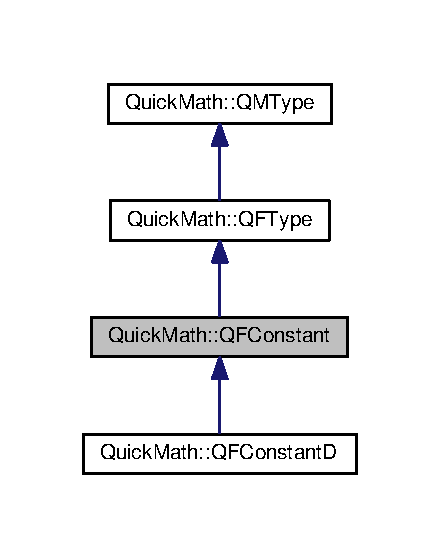
\includegraphics[width=211pt]{classQuickMath_1_1QFConstant__inherit__graph}
\end{center}
\end{figure}


Collaboration diagram for Quick\+Math\+:\+:Q\+F\+Constant\+:
\nopagebreak
\begin{figure}[H]
\begin{center}
\leavevmode
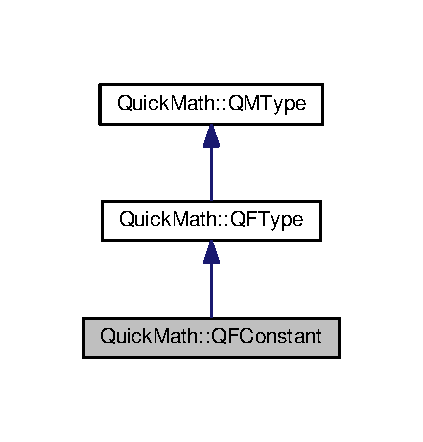
\includegraphics[width=203pt]{classQuickMath_1_1QFConstant__coll__graph}
\end{center}
\end{figure}
\subsection*{Private Member Functions}
\begin{DoxyCompactItemize}
\item 
bool \hyperlink{classQuickMath_1_1QFConstant_a399cf24d028b1536b4174ce9722834a4}{is\+Constant} () const 
\end{DoxyCompactItemize}
\subsection*{Additional Inherited Members}


\subsection{Member Function Documentation}
\hypertarget{classQuickMath_1_1QFConstant_a399cf24d028b1536b4174ce9722834a4}{}\index{Quick\+Math\+::\+Q\+F\+Constant@{Quick\+Math\+::\+Q\+F\+Constant}!is\+Constant@{is\+Constant}}
\index{is\+Constant@{is\+Constant}!Quick\+Math\+::\+Q\+F\+Constant@{Quick\+Math\+::\+Q\+F\+Constant}}
\subsubsection[{is\+Constant}]{\setlength{\rightskip}{0pt plus 5cm}bool Quick\+Math\+::\+Q\+F\+Constant\+::is\+Constant (
\begin{DoxyParamCaption}
{}
\end{DoxyParamCaption}
) const\hspace{0.3cm}{\ttfamily [private]}, {\ttfamily [virtual]}}\label{classQuickMath_1_1QFConstant_a399cf24d028b1536b4174ce9722834a4}


Reimplemented from \hyperlink{classQuickMath_1_1QFType_afe73e0f8bf974bccb2585f21f96375dc}{Quick\+Math\+::\+Q\+F\+Type}.



The documentation for this class was generated from the following files\+:\begin{DoxyCompactItemize}
\item 
include/\+Q\+Func/\hyperlink{QFConstant_8h}{Q\+F\+Constant.\+h}\item 
src/\+Q\+Func/\hyperlink{QFConstant_8cpp}{Q\+F\+Constant.\+cpp}\end{DoxyCompactItemize}

\hypertarget{classQuickMath_1_1QFConstantD}{}\section{Quick\+Math\+:\+:Q\+F\+Constant\+D Class Reference}
\label{classQuickMath_1_1QFConstantD}\index{Quick\+Math\+::\+Q\+F\+Constant\+D@{Quick\+Math\+::\+Q\+F\+Constant\+D}}


{\ttfamily \#include $<$Q\+F\+Constant\+D.\+h$>$}



Inheritance diagram for Quick\+Math\+:\+:Q\+F\+Constant\+D\+:
\nopagebreak
\begin{figure}[H]
\begin{center}
\leavevmode
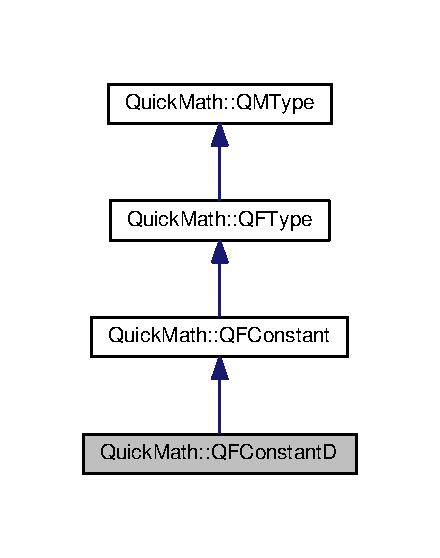
\includegraphics[width=211pt]{classQuickMath_1_1QFConstantD__inherit__graph}
\end{center}
\end{figure}


Collaboration diagram for Quick\+Math\+:\+:Q\+F\+Constant\+D\+:
\nopagebreak
\begin{figure}[H]
\begin{center}
\leavevmode
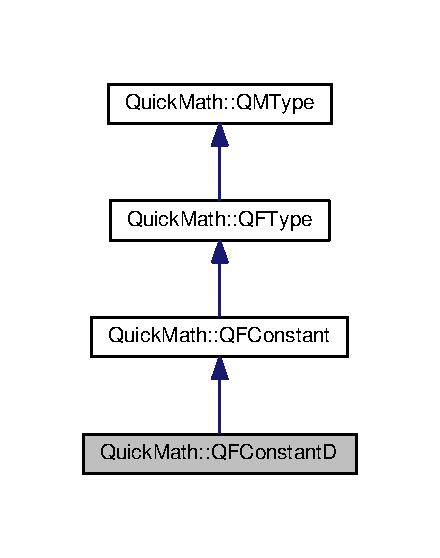
\includegraphics[width=211pt]{classQuickMath_1_1QFConstantD__coll__graph}
\end{center}
\end{figure}
\subsection*{Public Member Functions}
\begin{DoxyCompactItemize}
\item 
\hyperlink{classQuickMath_1_1QFConstantD_a1cdc74540910676597be00225bc30b01}{Q\+F\+Constant\+D} ()=default
\item 
\hyperlink{classQuickMath_1_1QFConstantD_a635e674bb35718825c2f8ae9238ac35a}{Q\+F\+Constant\+D} (double val)
\item 
\hyperlink{classQuickMath_1_1QFConstantD_af9be7ec600ff665ca734ac34cd4fd7d9}{Q\+F\+Constant\+D} (const \hyperlink{classQuickMath_1_1QFConstantD}{Q\+F\+Constant\+D} \&other)
\item 
std\+::unique\+\_\+ptr$<$ \hyperlink{classQuickMath_1_1QMType}{Q\+M\+Type} $>$ \hyperlink{classQuickMath_1_1QFConstantD_ae169fdb14208a3edb0d736051d9e096c}{clone} () const 
\item 
std\+::string \hyperlink{classQuickMath_1_1QFConstantD_a355ad05761ac9e917517eeb9762bceab}{to\+String} () const 
\end{DoxyCompactItemize}
\subsection*{Private Attributes}
\begin{DoxyCompactItemize}
\item 
double \hyperlink{classQuickMath_1_1QFConstantD_a781fcdc69f914d33771c406dc0497ad6}{value}
\end{DoxyCompactItemize}


\subsection{Constructor \& Destructor Documentation}
\hypertarget{classQuickMath_1_1QFConstantD_a1cdc74540910676597be00225bc30b01}{}\index{Quick\+Math\+::\+Q\+F\+Constant\+D@{Quick\+Math\+::\+Q\+F\+Constant\+D}!Q\+F\+Constant\+D@{Q\+F\+Constant\+D}}
\index{Q\+F\+Constant\+D@{Q\+F\+Constant\+D}!Quick\+Math\+::\+Q\+F\+Constant\+D@{Quick\+Math\+::\+Q\+F\+Constant\+D}}
\subsubsection[{Q\+F\+Constant\+D}]{\setlength{\rightskip}{0pt plus 5cm}Quick\+Math\+::\+Q\+F\+Constant\+D\+::\+Q\+F\+Constant\+D (
\begin{DoxyParamCaption}
{}
\end{DoxyParamCaption}
)\hspace{0.3cm}{\ttfamily [default]}}\label{classQuickMath_1_1QFConstantD_a1cdc74540910676597be00225bc30b01}
\hypertarget{classQuickMath_1_1QFConstantD_a635e674bb35718825c2f8ae9238ac35a}{}\index{Quick\+Math\+::\+Q\+F\+Constant\+D@{Quick\+Math\+::\+Q\+F\+Constant\+D}!Q\+F\+Constant\+D@{Q\+F\+Constant\+D}}
\index{Q\+F\+Constant\+D@{Q\+F\+Constant\+D}!Quick\+Math\+::\+Q\+F\+Constant\+D@{Quick\+Math\+::\+Q\+F\+Constant\+D}}
\subsubsection[{Q\+F\+Constant\+D}]{\setlength{\rightskip}{0pt plus 5cm}Quick\+Math\+::\+Q\+F\+Constant\+D\+::\+Q\+F\+Constant\+D (
\begin{DoxyParamCaption}
\item[{double}]{val}
\end{DoxyParamCaption}
)}\label{classQuickMath_1_1QFConstantD_a635e674bb35718825c2f8ae9238ac35a}
\hypertarget{classQuickMath_1_1QFConstantD_af9be7ec600ff665ca734ac34cd4fd7d9}{}\index{Quick\+Math\+::\+Q\+F\+Constant\+D@{Quick\+Math\+::\+Q\+F\+Constant\+D}!Q\+F\+Constant\+D@{Q\+F\+Constant\+D}}
\index{Q\+F\+Constant\+D@{Q\+F\+Constant\+D}!Quick\+Math\+::\+Q\+F\+Constant\+D@{Quick\+Math\+::\+Q\+F\+Constant\+D}}
\subsubsection[{Q\+F\+Constant\+D}]{\setlength{\rightskip}{0pt plus 5cm}Quick\+Math\+::\+Q\+F\+Constant\+D\+::\+Q\+F\+Constant\+D (
\begin{DoxyParamCaption}
\item[{const {\bf Q\+F\+Constant\+D} \&}]{other}
\end{DoxyParamCaption}
)}\label{classQuickMath_1_1QFConstantD_af9be7ec600ff665ca734ac34cd4fd7d9}


\subsection{Member Function Documentation}
\hypertarget{classQuickMath_1_1QFConstantD_ae169fdb14208a3edb0d736051d9e096c}{}\index{Quick\+Math\+::\+Q\+F\+Constant\+D@{Quick\+Math\+::\+Q\+F\+Constant\+D}!clone@{clone}}
\index{clone@{clone}!Quick\+Math\+::\+Q\+F\+Constant\+D@{Quick\+Math\+::\+Q\+F\+Constant\+D}}
\subsubsection[{clone}]{\setlength{\rightskip}{0pt plus 5cm}std\+::unique\+\_\+ptr$<$ {\bf Q\+M\+Type} $>$ Quick\+Math\+::\+Q\+F\+Constant\+D\+::clone (
\begin{DoxyParamCaption}
{}
\end{DoxyParamCaption}
) const\hspace{0.3cm}{\ttfamily [virtual]}}\label{classQuickMath_1_1QFConstantD_ae169fdb14208a3edb0d736051d9e096c}


Implements \hyperlink{classQuickMath_1_1QMType_a15b2a74a662417da99c6da9b7aaeff77}{Quick\+Math\+::\+Q\+M\+Type}.

\hypertarget{classQuickMath_1_1QFConstantD_a355ad05761ac9e917517eeb9762bceab}{}\index{Quick\+Math\+::\+Q\+F\+Constant\+D@{Quick\+Math\+::\+Q\+F\+Constant\+D}!to\+String@{to\+String}}
\index{to\+String@{to\+String}!Quick\+Math\+::\+Q\+F\+Constant\+D@{Quick\+Math\+::\+Q\+F\+Constant\+D}}
\subsubsection[{to\+String}]{\setlength{\rightskip}{0pt plus 5cm}std\+::string Quick\+Math\+::\+Q\+F\+Constant\+D\+::to\+String (
\begin{DoxyParamCaption}
{}
\end{DoxyParamCaption}
) const\hspace{0.3cm}{\ttfamily [virtual]}}\label{classQuickMath_1_1QFConstantD_a355ad05761ac9e917517eeb9762bceab}


Implements \hyperlink{classQuickMath_1_1QMType_a031b83c87e4edae28c65adf8e268442b}{Quick\+Math\+::\+Q\+M\+Type}.



\subsection{Member Data Documentation}
\hypertarget{classQuickMath_1_1QFConstantD_a781fcdc69f914d33771c406dc0497ad6}{}\index{Quick\+Math\+::\+Q\+F\+Constant\+D@{Quick\+Math\+::\+Q\+F\+Constant\+D}!value@{value}}
\index{value@{value}!Quick\+Math\+::\+Q\+F\+Constant\+D@{Quick\+Math\+::\+Q\+F\+Constant\+D}}
\subsubsection[{value}]{\setlength{\rightskip}{0pt plus 5cm}double Quick\+Math\+::\+Q\+F\+Constant\+D\+::value\hspace{0.3cm}{\ttfamily [private]}}\label{classQuickMath_1_1QFConstantD_a781fcdc69f914d33771c406dc0497ad6}


The documentation for this class was generated from the following files\+:\begin{DoxyCompactItemize}
\item 
include/\+Q\+Func/\hyperlink{QFConstantD_8h}{Q\+F\+Constant\+D.\+h}\item 
src/\+Q\+Func/\hyperlink{QFConstantD_8cpp}{Q\+F\+Constant\+D.\+cpp}\end{DoxyCompactItemize}

\hypertarget{classQuickMath_1_1QFExpr}{}\section{Quick\+Math\+:\+:Q\+F\+Expr Class Reference}
\label{classQuickMath_1_1QFExpr}\index{Quick\+Math\+::\+Q\+F\+Expr@{Quick\+Math\+::\+Q\+F\+Expr}}


{\ttfamily \#include $<$Q\+F\+Expr.\+h$>$}



Inheritance diagram for Quick\+Math\+:\+:Q\+F\+Expr\+:
\nopagebreak
\begin{figure}[H]
\begin{center}
\leavevmode
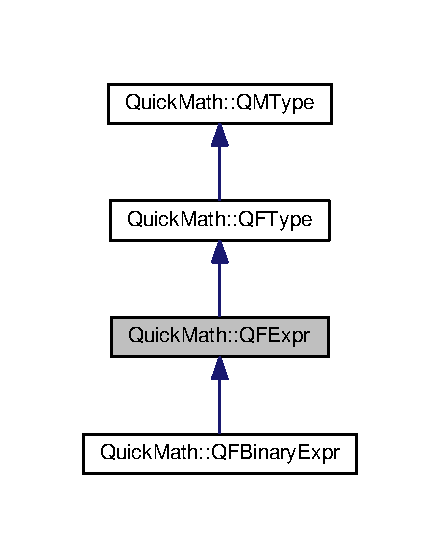
\includegraphics[width=211pt]{classQuickMath_1_1QFExpr__inherit__graph}
\end{center}
\end{figure}


Collaboration diagram for Quick\+Math\+:\+:Q\+F\+Expr\+:
\nopagebreak
\begin{figure}[H]
\begin{center}
\leavevmode
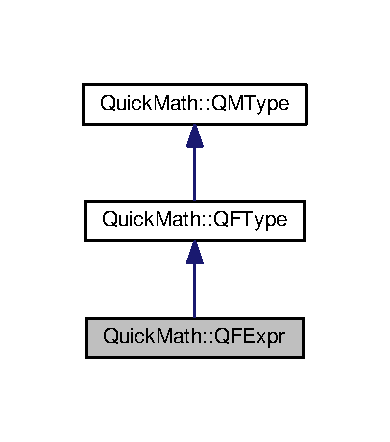
\includegraphics[width=187pt]{classQuickMath_1_1QFExpr__coll__graph}
\end{center}
\end{figure}
\subsection*{Public Member Functions}
\begin{DoxyCompactItemize}
\item 
bool \hyperlink{classQuickMath_1_1QFExpr_a71774ec9d7ae0aa7d06b2db9a4d20334}{is\+Expr} () const 
\item 
virtual \hyperlink{namespaceQuickMath_a0a6c67b9dab0cfd5f3e711b0573545cb}{Q\+M\+Op\+Type} \hyperlink{classQuickMath_1_1QFExpr_a9a91cb4d8269ad109591c8311288f487}{op\+Type} () const 
\end{DoxyCompactItemize}
\subsection*{Protected Attributes}
\begin{DoxyCompactItemize}
\item 
\hyperlink{namespaceQuickMath_a0a6c67b9dab0cfd5f3e711b0573545cb}{Q\+M\+Op\+Type} \hyperlink{classQuickMath_1_1QFExpr_afbd5672bd261cdf4d60a4c0b5a142820}{op}
\end{DoxyCompactItemize}


\subsection{Member Function Documentation}
\hypertarget{classQuickMath_1_1QFExpr_a71774ec9d7ae0aa7d06b2db9a4d20334}{}\index{Quick\+Math\+::\+Q\+F\+Expr@{Quick\+Math\+::\+Q\+F\+Expr}!is\+Expr@{is\+Expr}}
\index{is\+Expr@{is\+Expr}!Quick\+Math\+::\+Q\+F\+Expr@{Quick\+Math\+::\+Q\+F\+Expr}}
\subsubsection[{is\+Expr}]{\setlength{\rightskip}{0pt plus 5cm}bool Quick\+Math\+::\+Q\+F\+Expr\+::is\+Expr (
\begin{DoxyParamCaption}
{}
\end{DoxyParamCaption}
) const\hspace{0.3cm}{\ttfamily [virtual]}}\label{classQuickMath_1_1QFExpr_a71774ec9d7ae0aa7d06b2db9a4d20334}


Reimplemented from \hyperlink{classQuickMath_1_1QFType_aedcccde5d0e2b2b8b52545bc511a6b1a}{Quick\+Math\+::\+Q\+F\+Type}.

\hypertarget{classQuickMath_1_1QFExpr_a9a91cb4d8269ad109591c8311288f487}{}\index{Quick\+Math\+::\+Q\+F\+Expr@{Quick\+Math\+::\+Q\+F\+Expr}!op\+Type@{op\+Type}}
\index{op\+Type@{op\+Type}!Quick\+Math\+::\+Q\+F\+Expr@{Quick\+Math\+::\+Q\+F\+Expr}}
\subsubsection[{op\+Type}]{\setlength{\rightskip}{0pt plus 5cm}{\bf Q\+M\+Op\+Type} Quick\+Math\+::\+Q\+F\+Expr\+::op\+Type (
\begin{DoxyParamCaption}
{}
\end{DoxyParamCaption}
) const\hspace{0.3cm}{\ttfamily [virtual]}}\label{classQuickMath_1_1QFExpr_a9a91cb4d8269ad109591c8311288f487}


\subsection{Member Data Documentation}
\hypertarget{classQuickMath_1_1QFExpr_afbd5672bd261cdf4d60a4c0b5a142820}{}\index{Quick\+Math\+::\+Q\+F\+Expr@{Quick\+Math\+::\+Q\+F\+Expr}!op@{op}}
\index{op@{op}!Quick\+Math\+::\+Q\+F\+Expr@{Quick\+Math\+::\+Q\+F\+Expr}}
\subsubsection[{op}]{\setlength{\rightskip}{0pt plus 5cm}{\bf Q\+M\+Op\+Type} Quick\+Math\+::\+Q\+F\+Expr\+::op\hspace{0.3cm}{\ttfamily [protected]}}\label{classQuickMath_1_1QFExpr_afbd5672bd261cdf4d60a4c0b5a142820}


The documentation for this class was generated from the following files\+:\begin{DoxyCompactItemize}
\item 
include/\+Q\+Func/\hyperlink{QFExpr_8h}{Q\+F\+Expr.\+h}\item 
src/\+Q\+Func/\hyperlink{QFExpr_8cpp}{Q\+F\+Expr.\+cpp}\end{DoxyCompactItemize}

\hypertarget{classQuickMath_1_1QFType}{}\section{Quick\+Math\+:\+:Q\+F\+Type Class Reference}
\label{classQuickMath_1_1QFType}\index{Quick\+Math\+::\+Q\+F\+Type@{Quick\+Math\+::\+Q\+F\+Type}}


{\ttfamily \#include $<$Q\+F\+Type.\+h$>$}



Inheritance diagram for Quick\+Math\+:\+:Q\+F\+Type\+:
\nopagebreak
\begin{figure}[H]
\begin{center}
\leavevmode
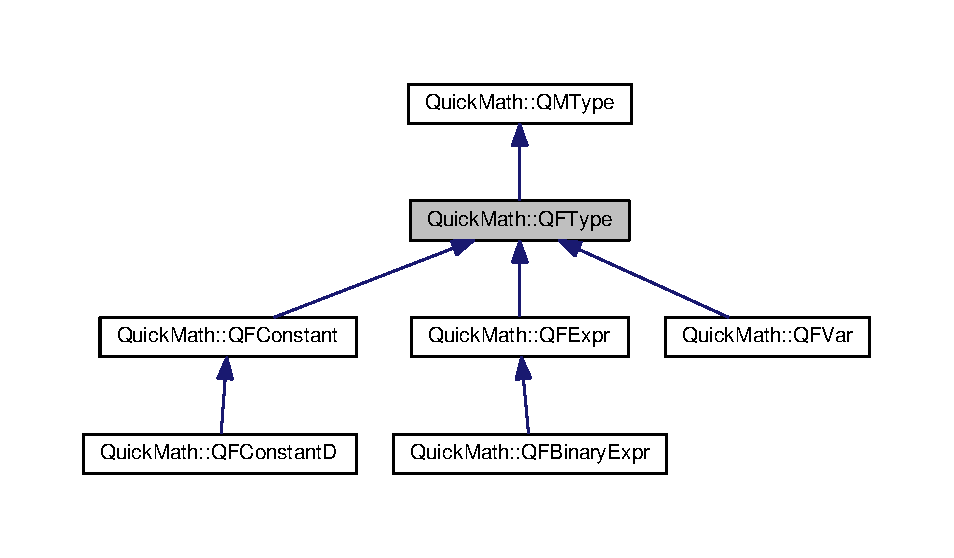
\includegraphics[width=350pt]{classQuickMath_1_1QFType__inherit__graph}
\end{center}
\end{figure}


Collaboration diagram for Quick\+Math\+:\+:Q\+F\+Type\+:
\nopagebreak
\begin{figure}[H]
\begin{center}
\leavevmode
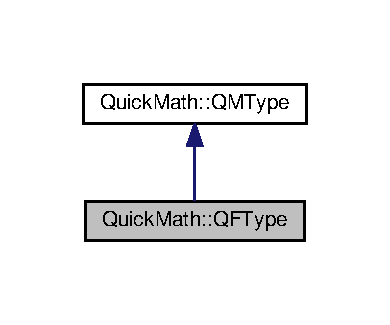
\includegraphics[width=187pt]{classQuickMath_1_1QFType__coll__graph}
\end{center}
\end{figure}
\subsection*{Public Member Functions}
\begin{DoxyCompactItemize}
\item 
bool \hyperlink{classQuickMath_1_1QFType_a827446c95b66123a6f6cb31087b71ffd}{is\+Func\+Type} () const 
\item 
virtual bool \hyperlink{classQuickMath_1_1QFType_ad78ec900922425e3a7d6249107704379}{is\+Var} () const 
\item 
virtual bool \hyperlink{classQuickMath_1_1QFType_aedcccde5d0e2b2b8b52545bc511a6b1a}{is\+Expr} () const 
\item 
virtual bool \hyperlink{classQuickMath_1_1QFType_afe73e0f8bf974bccb2585f21f96375dc}{is\+Constant} () const 
\end{DoxyCompactItemize}


\subsection{Member Function Documentation}
\hypertarget{classQuickMath_1_1QFType_afe73e0f8bf974bccb2585f21f96375dc}{}\index{Quick\+Math\+::\+Q\+F\+Type@{Quick\+Math\+::\+Q\+F\+Type}!is\+Constant@{is\+Constant}}
\index{is\+Constant@{is\+Constant}!Quick\+Math\+::\+Q\+F\+Type@{Quick\+Math\+::\+Q\+F\+Type}}
\subsubsection[{is\+Constant}]{\setlength{\rightskip}{0pt plus 5cm}virtual bool Quick\+Math\+::\+Q\+F\+Type\+::is\+Constant (
\begin{DoxyParamCaption}
{}
\end{DoxyParamCaption}
) const\hspace{0.3cm}{\ttfamily [inline]}, {\ttfamily [virtual]}}\label{classQuickMath_1_1QFType_afe73e0f8bf974bccb2585f21f96375dc}


Reimplemented in \hyperlink{classQuickMath_1_1QFConstant_a399cf24d028b1536b4174ce9722834a4}{Quick\+Math\+::\+Q\+F\+Constant}.

\hypertarget{classQuickMath_1_1QFType_aedcccde5d0e2b2b8b52545bc511a6b1a}{}\index{Quick\+Math\+::\+Q\+F\+Type@{Quick\+Math\+::\+Q\+F\+Type}!is\+Expr@{is\+Expr}}
\index{is\+Expr@{is\+Expr}!Quick\+Math\+::\+Q\+F\+Type@{Quick\+Math\+::\+Q\+F\+Type}}
\subsubsection[{is\+Expr}]{\setlength{\rightskip}{0pt plus 5cm}virtual bool Quick\+Math\+::\+Q\+F\+Type\+::is\+Expr (
\begin{DoxyParamCaption}
{}
\end{DoxyParamCaption}
) const\hspace{0.3cm}{\ttfamily [inline]}, {\ttfamily [virtual]}}\label{classQuickMath_1_1QFType_aedcccde5d0e2b2b8b52545bc511a6b1a}


Reimplemented in \hyperlink{classQuickMath_1_1QFExpr_a71774ec9d7ae0aa7d06b2db9a4d20334}{Quick\+Math\+::\+Q\+F\+Expr}.

\hypertarget{classQuickMath_1_1QFType_a827446c95b66123a6f6cb31087b71ffd}{}\index{Quick\+Math\+::\+Q\+F\+Type@{Quick\+Math\+::\+Q\+F\+Type}!is\+Func\+Type@{is\+Func\+Type}}
\index{is\+Func\+Type@{is\+Func\+Type}!Quick\+Math\+::\+Q\+F\+Type@{Quick\+Math\+::\+Q\+F\+Type}}
\subsubsection[{is\+Func\+Type}]{\setlength{\rightskip}{0pt plus 5cm}bool Quick\+Math\+::\+Q\+F\+Type\+::is\+Func\+Type (
\begin{DoxyParamCaption}
{}
\end{DoxyParamCaption}
) const\hspace{0.3cm}{\ttfamily [inline]}, {\ttfamily [virtual]}}\label{classQuickMath_1_1QFType_a827446c95b66123a6f6cb31087b71ffd}


Reimplemented from \hyperlink{classQuickMath_1_1QMType_ae9dc3e4b23d53df761e17625688ae404}{Quick\+Math\+::\+Q\+M\+Type}.

\hypertarget{classQuickMath_1_1QFType_ad78ec900922425e3a7d6249107704379}{}\index{Quick\+Math\+::\+Q\+F\+Type@{Quick\+Math\+::\+Q\+F\+Type}!is\+Var@{is\+Var}}
\index{is\+Var@{is\+Var}!Quick\+Math\+::\+Q\+F\+Type@{Quick\+Math\+::\+Q\+F\+Type}}
\subsubsection[{is\+Var}]{\setlength{\rightskip}{0pt plus 5cm}virtual bool Quick\+Math\+::\+Q\+F\+Type\+::is\+Var (
\begin{DoxyParamCaption}
{}
\end{DoxyParamCaption}
) const\hspace{0.3cm}{\ttfamily [inline]}, {\ttfamily [virtual]}}\label{classQuickMath_1_1QFType_ad78ec900922425e3a7d6249107704379}


Reimplemented in \hyperlink{classQuickMath_1_1QFVar_a1e5a49b3cce6d8d14af56f23a88ea01d}{Quick\+Math\+::\+Q\+F\+Var}.



The documentation for this class was generated from the following file\+:\begin{DoxyCompactItemize}
\item 
include/\+Q\+Func/\hyperlink{QFType_8h}{Q\+F\+Type.\+h}\end{DoxyCompactItemize}

\hypertarget{classQuickMath_1_1QFVar}{}\section{Quick\+Math\+:\+:Q\+F\+Var Class Reference}
\label{classQuickMath_1_1QFVar}\index{Quick\+Math\+::\+Q\+F\+Var@{Quick\+Math\+::\+Q\+F\+Var}}


{\ttfamily \#include $<$Q\+F\+Var.\+h$>$}



Inheritance diagram for Quick\+Math\+:\+:Q\+F\+Var\+:
\nopagebreak
\begin{figure}[H]
\begin{center}
\leavevmode
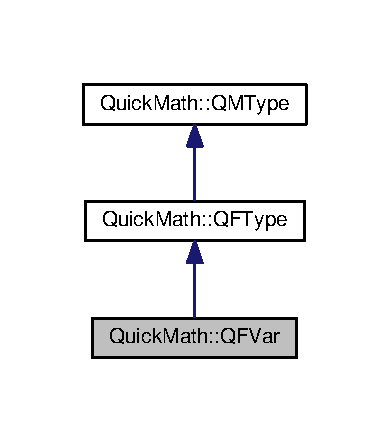
\includegraphics[width=187pt]{classQuickMath_1_1QFVar__inherit__graph}
\end{center}
\end{figure}


Collaboration diagram for Quick\+Math\+:\+:Q\+F\+Var\+:
\nopagebreak
\begin{figure}[H]
\begin{center}
\leavevmode
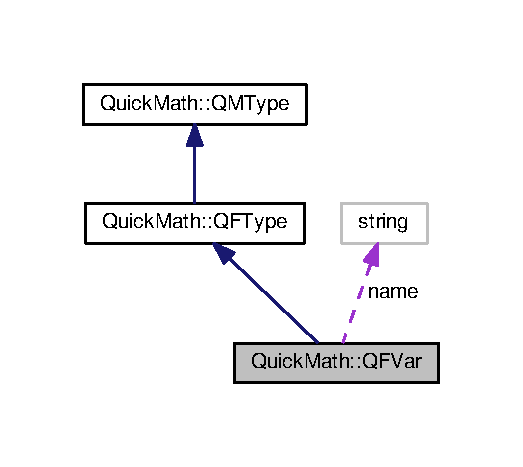
\includegraphics[width=251pt]{classQuickMath_1_1QFVar__coll__graph}
\end{center}
\end{figure}
\subsection*{Public Member Functions}
\begin{DoxyCompactItemize}
\item 
\hyperlink{classQuickMath_1_1QFVar_a676bc9879b6d6079800060d2554080b2}{Q\+F\+Var} ()=default
\item 
\hyperlink{classQuickMath_1_1QFVar_a9013e1baba39838798a9f5eaccb25e2a}{Q\+F\+Var} (const std\+::string \&\hyperlink{classQuickMath_1_1QFVar_a39703d5b8aa86d92e22b344e92ccfd77}{name}, int \hyperlink{classQuickMath_1_1QFVar_ac878e4d5217813ee3fca965a9f6a6b1c}{idx}=0)
\item 
\hyperlink{classQuickMath_1_1QFVar_af95d9389974eff58ac4422f0757835a2}{Q\+F\+Var} (const \hyperlink{classQuickMath_1_1QFVar}{Q\+F\+Var} \&var)
\item 
\hyperlink{classQuickMath_1_1QFVar_ad700d482b2e7a0d6c4d2a8b9dcf416a0}{Q\+F\+Var} (\hyperlink{classQuickMath_1_1QFVar}{Q\+F\+Var} \&\&var)
\item 
\hyperlink{classQuickMath_1_1QFVar}{Q\+F\+Var} \& \hyperlink{classQuickMath_1_1QFVar_a96ae8db7661f61f4e17e5c14cc1ff7c8}{operator=} (const \hyperlink{classQuickMath_1_1QFVar}{Q\+F\+Var} \&other)
\item 
\hyperlink{classQuickMath_1_1QFVar}{Q\+F\+Var} \& \hyperlink{classQuickMath_1_1QFVar_af4d5f5644a7b53cd4f5eb72a9a2df3f4}{operator=} (\hyperlink{classQuickMath_1_1QFVar}{Q\+F\+Var} \&\&other)
\item 
std\+::unique\+\_\+ptr$<$ \hyperlink{classQuickMath_1_1QMType}{Q\+M\+Type} $>$ \hyperlink{classQuickMath_1_1QFVar_a07f3155c995f0cd7dfee1dca2c8ca4d6}{clone} () const 
\item 
std\+::string \hyperlink{classQuickMath_1_1QFVar_a13ed0152f1920b3d7b0f4c86b64d0333}{to\+String} () const 
\item 
bool \hyperlink{classQuickMath_1_1QFVar_a1e5a49b3cce6d8d14af56f23a88ea01d}{is\+Var} () const 
\item 
const std\+::string \& \hyperlink{classQuickMath_1_1QFVar_a5940092ea947a3069a53a7a279062fbc}{get\+Name} () const 
\item 
int \hyperlink{classQuickMath_1_1QFVar_ae12ac2261ad4bf78ec5e21db5ca3b4e3}{get\+Index} () const 
\item 
bool \hyperlink{classQuickMath_1_1QFVar_a9a42646ecb85e763ce5eb5e0661df47a}{operator==} (const \hyperlink{classQuickMath_1_1QFVar}{Q\+F\+Var} \&rhs) const 
\item 
bool \hyperlink{classQuickMath_1_1QFVar_a37631d1bc1d43d0a26287caacb5996e1}{operator$<$} (const \hyperlink{classQuickMath_1_1QFVar}{Q\+F\+Var} \&rhs) const 
\item 
virtual \hyperlink{classQuickMath_1_1QFVar_aeddabc1cf78d984b41314eba81376b79}{$\sim$\+Q\+F\+Var} ()
\end{DoxyCompactItemize}
\subsection*{Private Attributes}
\begin{DoxyCompactItemize}
\item 
std\+::string \hyperlink{classQuickMath_1_1QFVar_a39703d5b8aa86d92e22b344e92ccfd77}{name}
\item 
int \hyperlink{classQuickMath_1_1QFVar_ac878e4d5217813ee3fca965a9f6a6b1c}{idx} = 0
\end{DoxyCompactItemize}


\subsection{Constructor \& Destructor Documentation}
\hypertarget{classQuickMath_1_1QFVar_a676bc9879b6d6079800060d2554080b2}{}\index{Quick\+Math\+::\+Q\+F\+Var@{Quick\+Math\+::\+Q\+F\+Var}!Q\+F\+Var@{Q\+F\+Var}}
\index{Q\+F\+Var@{Q\+F\+Var}!Quick\+Math\+::\+Q\+F\+Var@{Quick\+Math\+::\+Q\+F\+Var}}
\subsubsection[{Q\+F\+Var}]{\setlength{\rightskip}{0pt plus 5cm}Quick\+Math\+::\+Q\+F\+Var\+::\+Q\+F\+Var (
\begin{DoxyParamCaption}
{}
\end{DoxyParamCaption}
)\hspace{0.3cm}{\ttfamily [default]}}\label{classQuickMath_1_1QFVar_a676bc9879b6d6079800060d2554080b2}
\hypertarget{classQuickMath_1_1QFVar_a9013e1baba39838798a9f5eaccb25e2a}{}\index{Quick\+Math\+::\+Q\+F\+Var@{Quick\+Math\+::\+Q\+F\+Var}!Q\+F\+Var@{Q\+F\+Var}}
\index{Q\+F\+Var@{Q\+F\+Var}!Quick\+Math\+::\+Q\+F\+Var@{Quick\+Math\+::\+Q\+F\+Var}}
\subsubsection[{Q\+F\+Var}]{\setlength{\rightskip}{0pt plus 5cm}Quick\+Math\+::\+Q\+F\+Var\+::\+Q\+F\+Var (
\begin{DoxyParamCaption}
\item[{const std\+::string \&}]{name, }
\item[{int}]{idx = {\ttfamily 0}}
\end{DoxyParamCaption}
)}\label{classQuickMath_1_1QFVar_a9013e1baba39838798a9f5eaccb25e2a}
\hypertarget{classQuickMath_1_1QFVar_af95d9389974eff58ac4422f0757835a2}{}\index{Quick\+Math\+::\+Q\+F\+Var@{Quick\+Math\+::\+Q\+F\+Var}!Q\+F\+Var@{Q\+F\+Var}}
\index{Q\+F\+Var@{Q\+F\+Var}!Quick\+Math\+::\+Q\+F\+Var@{Quick\+Math\+::\+Q\+F\+Var}}
\subsubsection[{Q\+F\+Var}]{\setlength{\rightskip}{0pt plus 5cm}Quick\+Math\+::\+Q\+F\+Var\+::\+Q\+F\+Var (
\begin{DoxyParamCaption}
\item[{const {\bf Q\+F\+Var} \&}]{var}
\end{DoxyParamCaption}
)}\label{classQuickMath_1_1QFVar_af95d9389974eff58ac4422f0757835a2}
\hypertarget{classQuickMath_1_1QFVar_ad700d482b2e7a0d6c4d2a8b9dcf416a0}{}\index{Quick\+Math\+::\+Q\+F\+Var@{Quick\+Math\+::\+Q\+F\+Var}!Q\+F\+Var@{Q\+F\+Var}}
\index{Q\+F\+Var@{Q\+F\+Var}!Quick\+Math\+::\+Q\+F\+Var@{Quick\+Math\+::\+Q\+F\+Var}}
\subsubsection[{Q\+F\+Var}]{\setlength{\rightskip}{0pt plus 5cm}Quick\+Math\+::\+Q\+F\+Var\+::\+Q\+F\+Var (
\begin{DoxyParamCaption}
\item[{{\bf Q\+F\+Var} \&\&}]{var}
\end{DoxyParamCaption}
)}\label{classQuickMath_1_1QFVar_ad700d482b2e7a0d6c4d2a8b9dcf416a0}
\hypertarget{classQuickMath_1_1QFVar_aeddabc1cf78d984b41314eba81376b79}{}\index{Quick\+Math\+::\+Q\+F\+Var@{Quick\+Math\+::\+Q\+F\+Var}!````~Q\+F\+Var@{$\sim$\+Q\+F\+Var}}
\index{````~Q\+F\+Var@{$\sim$\+Q\+F\+Var}!Quick\+Math\+::\+Q\+F\+Var@{Quick\+Math\+::\+Q\+F\+Var}}
\subsubsection[{$\sim$\+Q\+F\+Var}]{\setlength{\rightskip}{0pt plus 5cm}Quick\+Math\+::\+Q\+F\+Var\+::$\sim$\+Q\+F\+Var (
\begin{DoxyParamCaption}
{}
\end{DoxyParamCaption}
)\hspace{0.3cm}{\ttfamily [virtual]}}\label{classQuickMath_1_1QFVar_aeddabc1cf78d984b41314eba81376b79}


\subsection{Member Function Documentation}
\hypertarget{classQuickMath_1_1QFVar_a07f3155c995f0cd7dfee1dca2c8ca4d6}{}\index{Quick\+Math\+::\+Q\+F\+Var@{Quick\+Math\+::\+Q\+F\+Var}!clone@{clone}}
\index{clone@{clone}!Quick\+Math\+::\+Q\+F\+Var@{Quick\+Math\+::\+Q\+F\+Var}}
\subsubsection[{clone}]{\setlength{\rightskip}{0pt plus 5cm}std\+::unique\+\_\+ptr$<$ {\bf Q\+M\+Type} $>$ Quick\+Math\+::\+Q\+F\+Var\+::clone (
\begin{DoxyParamCaption}
{}
\end{DoxyParamCaption}
) const\hspace{0.3cm}{\ttfamily [virtual]}}\label{classQuickMath_1_1QFVar_a07f3155c995f0cd7dfee1dca2c8ca4d6}


Implements \hyperlink{classQuickMath_1_1QMType_a15b2a74a662417da99c6da9b7aaeff77}{Quick\+Math\+::\+Q\+M\+Type}.

\hypertarget{classQuickMath_1_1QFVar_ae12ac2261ad4bf78ec5e21db5ca3b4e3}{}\index{Quick\+Math\+::\+Q\+F\+Var@{Quick\+Math\+::\+Q\+F\+Var}!get\+Index@{get\+Index}}
\index{get\+Index@{get\+Index}!Quick\+Math\+::\+Q\+F\+Var@{Quick\+Math\+::\+Q\+F\+Var}}
\subsubsection[{get\+Index}]{\setlength{\rightskip}{0pt plus 5cm}int Quick\+Math\+::\+Q\+F\+Var\+::get\+Index (
\begin{DoxyParamCaption}
{}
\end{DoxyParamCaption}
) const}\label{classQuickMath_1_1QFVar_ae12ac2261ad4bf78ec5e21db5ca3b4e3}
\hypertarget{classQuickMath_1_1QFVar_a5940092ea947a3069a53a7a279062fbc}{}\index{Quick\+Math\+::\+Q\+F\+Var@{Quick\+Math\+::\+Q\+F\+Var}!get\+Name@{get\+Name}}
\index{get\+Name@{get\+Name}!Quick\+Math\+::\+Q\+F\+Var@{Quick\+Math\+::\+Q\+F\+Var}}
\subsubsection[{get\+Name}]{\setlength{\rightskip}{0pt plus 5cm}const std\+::string \& Quick\+Math\+::\+Q\+F\+Var\+::get\+Name (
\begin{DoxyParamCaption}
{}
\end{DoxyParamCaption}
) const}\label{classQuickMath_1_1QFVar_a5940092ea947a3069a53a7a279062fbc}
\hypertarget{classQuickMath_1_1QFVar_a1e5a49b3cce6d8d14af56f23a88ea01d}{}\index{Quick\+Math\+::\+Q\+F\+Var@{Quick\+Math\+::\+Q\+F\+Var}!is\+Var@{is\+Var}}
\index{is\+Var@{is\+Var}!Quick\+Math\+::\+Q\+F\+Var@{Quick\+Math\+::\+Q\+F\+Var}}
\subsubsection[{is\+Var}]{\setlength{\rightskip}{0pt plus 5cm}bool Quick\+Math\+::\+Q\+F\+Var\+::is\+Var (
\begin{DoxyParamCaption}
{}
\end{DoxyParamCaption}
) const\hspace{0.3cm}{\ttfamily [virtual]}}\label{classQuickMath_1_1QFVar_a1e5a49b3cce6d8d14af56f23a88ea01d}


Reimplemented from \hyperlink{classQuickMath_1_1QFType_ad78ec900922425e3a7d6249107704379}{Quick\+Math\+::\+Q\+F\+Type}.

\hypertarget{classQuickMath_1_1QFVar_a37631d1bc1d43d0a26287caacb5996e1}{}\index{Quick\+Math\+::\+Q\+F\+Var@{Quick\+Math\+::\+Q\+F\+Var}!operator$<$@{operator$<$}}
\index{operator$<$@{operator$<$}!Quick\+Math\+::\+Q\+F\+Var@{Quick\+Math\+::\+Q\+F\+Var}}
\subsubsection[{operator$<$}]{\setlength{\rightskip}{0pt plus 5cm}bool Quick\+Math\+::\+Q\+F\+Var\+::operator$<$ (
\begin{DoxyParamCaption}
\item[{const {\bf Q\+F\+Var} \&}]{rhs}
\end{DoxyParamCaption}
) const}\label{classQuickMath_1_1QFVar_a37631d1bc1d43d0a26287caacb5996e1}
\hypertarget{classQuickMath_1_1QFVar_a96ae8db7661f61f4e17e5c14cc1ff7c8}{}\index{Quick\+Math\+::\+Q\+F\+Var@{Quick\+Math\+::\+Q\+F\+Var}!operator=@{operator=}}
\index{operator=@{operator=}!Quick\+Math\+::\+Q\+F\+Var@{Quick\+Math\+::\+Q\+F\+Var}}
\subsubsection[{operator=}]{\setlength{\rightskip}{0pt plus 5cm}{\bf Q\+F\+Var} \& Quick\+Math\+::\+Q\+F\+Var\+::operator= (
\begin{DoxyParamCaption}
\item[{const {\bf Q\+F\+Var} \&}]{other}
\end{DoxyParamCaption}
)}\label{classQuickMath_1_1QFVar_a96ae8db7661f61f4e17e5c14cc1ff7c8}
\hypertarget{classQuickMath_1_1QFVar_af4d5f5644a7b53cd4f5eb72a9a2df3f4}{}\index{Quick\+Math\+::\+Q\+F\+Var@{Quick\+Math\+::\+Q\+F\+Var}!operator=@{operator=}}
\index{operator=@{operator=}!Quick\+Math\+::\+Q\+F\+Var@{Quick\+Math\+::\+Q\+F\+Var}}
\subsubsection[{operator=}]{\setlength{\rightskip}{0pt plus 5cm}{\bf Q\+F\+Var} \& Quick\+Math\+::\+Q\+F\+Var\+::operator= (
\begin{DoxyParamCaption}
\item[{{\bf Q\+F\+Var} \&\&}]{other}
\end{DoxyParamCaption}
)}\label{classQuickMath_1_1QFVar_af4d5f5644a7b53cd4f5eb72a9a2df3f4}
\hypertarget{classQuickMath_1_1QFVar_a9a42646ecb85e763ce5eb5e0661df47a}{}\index{Quick\+Math\+::\+Q\+F\+Var@{Quick\+Math\+::\+Q\+F\+Var}!operator==@{operator==}}
\index{operator==@{operator==}!Quick\+Math\+::\+Q\+F\+Var@{Quick\+Math\+::\+Q\+F\+Var}}
\subsubsection[{operator==}]{\setlength{\rightskip}{0pt plus 5cm}bool Quick\+Math\+::\+Q\+F\+Var\+::operator== (
\begin{DoxyParamCaption}
\item[{const {\bf Q\+F\+Var} \&}]{rhs}
\end{DoxyParamCaption}
) const}\label{classQuickMath_1_1QFVar_a9a42646ecb85e763ce5eb5e0661df47a}
\hypertarget{classQuickMath_1_1QFVar_a13ed0152f1920b3d7b0f4c86b64d0333}{}\index{Quick\+Math\+::\+Q\+F\+Var@{Quick\+Math\+::\+Q\+F\+Var}!to\+String@{to\+String}}
\index{to\+String@{to\+String}!Quick\+Math\+::\+Q\+F\+Var@{Quick\+Math\+::\+Q\+F\+Var}}
\subsubsection[{to\+String}]{\setlength{\rightskip}{0pt plus 5cm}std\+::string Quick\+Math\+::\+Q\+F\+Var\+::to\+String (
\begin{DoxyParamCaption}
{}
\end{DoxyParamCaption}
) const\hspace{0.3cm}{\ttfamily [virtual]}}\label{classQuickMath_1_1QFVar_a13ed0152f1920b3d7b0f4c86b64d0333}


Implements \hyperlink{classQuickMath_1_1QMType_a031b83c87e4edae28c65adf8e268442b}{Quick\+Math\+::\+Q\+M\+Type}.



\subsection{Member Data Documentation}
\hypertarget{classQuickMath_1_1QFVar_ac878e4d5217813ee3fca965a9f6a6b1c}{}\index{Quick\+Math\+::\+Q\+F\+Var@{Quick\+Math\+::\+Q\+F\+Var}!idx@{idx}}
\index{idx@{idx}!Quick\+Math\+::\+Q\+F\+Var@{Quick\+Math\+::\+Q\+F\+Var}}
\subsubsection[{idx}]{\setlength{\rightskip}{0pt plus 5cm}int Quick\+Math\+::\+Q\+F\+Var\+::idx = 0\hspace{0.3cm}{\ttfamily [private]}}\label{classQuickMath_1_1QFVar_ac878e4d5217813ee3fca965a9f6a6b1c}
\hypertarget{classQuickMath_1_1QFVar_a39703d5b8aa86d92e22b344e92ccfd77}{}\index{Quick\+Math\+::\+Q\+F\+Var@{Quick\+Math\+::\+Q\+F\+Var}!name@{name}}
\index{name@{name}!Quick\+Math\+::\+Q\+F\+Var@{Quick\+Math\+::\+Q\+F\+Var}}
\subsubsection[{name}]{\setlength{\rightskip}{0pt plus 5cm}std\+::string Quick\+Math\+::\+Q\+F\+Var\+::name\hspace{0.3cm}{\ttfamily [private]}}\label{classQuickMath_1_1QFVar_a39703d5b8aa86d92e22b344e92ccfd77}


The documentation for this class was generated from the following files\+:\begin{DoxyCompactItemize}
\item 
include/\+Q\+Func/\hyperlink{QFVar_8h}{Q\+F\+Var.\+h}\item 
src/\+Q\+Func/\hyperlink{QFVar_8cpp}{Q\+F\+Var.\+cpp}\end{DoxyCompactItemize}

\hypertarget{classQuickMath_1_1QMType}{}\section{Quick\+Math\+:\+:Q\+M\+Type Class Reference}
\label{classQuickMath_1_1QMType}\index{Quick\+Math\+::\+Q\+M\+Type@{Quick\+Math\+::\+Q\+M\+Type}}


{\ttfamily \#include $<$Q\+M\+Type.\+h$>$}



Inheritance diagram for Quick\+Math\+:\+:Q\+M\+Type\+:
\nopagebreak
\begin{figure}[H]
\begin{center}
\leavevmode
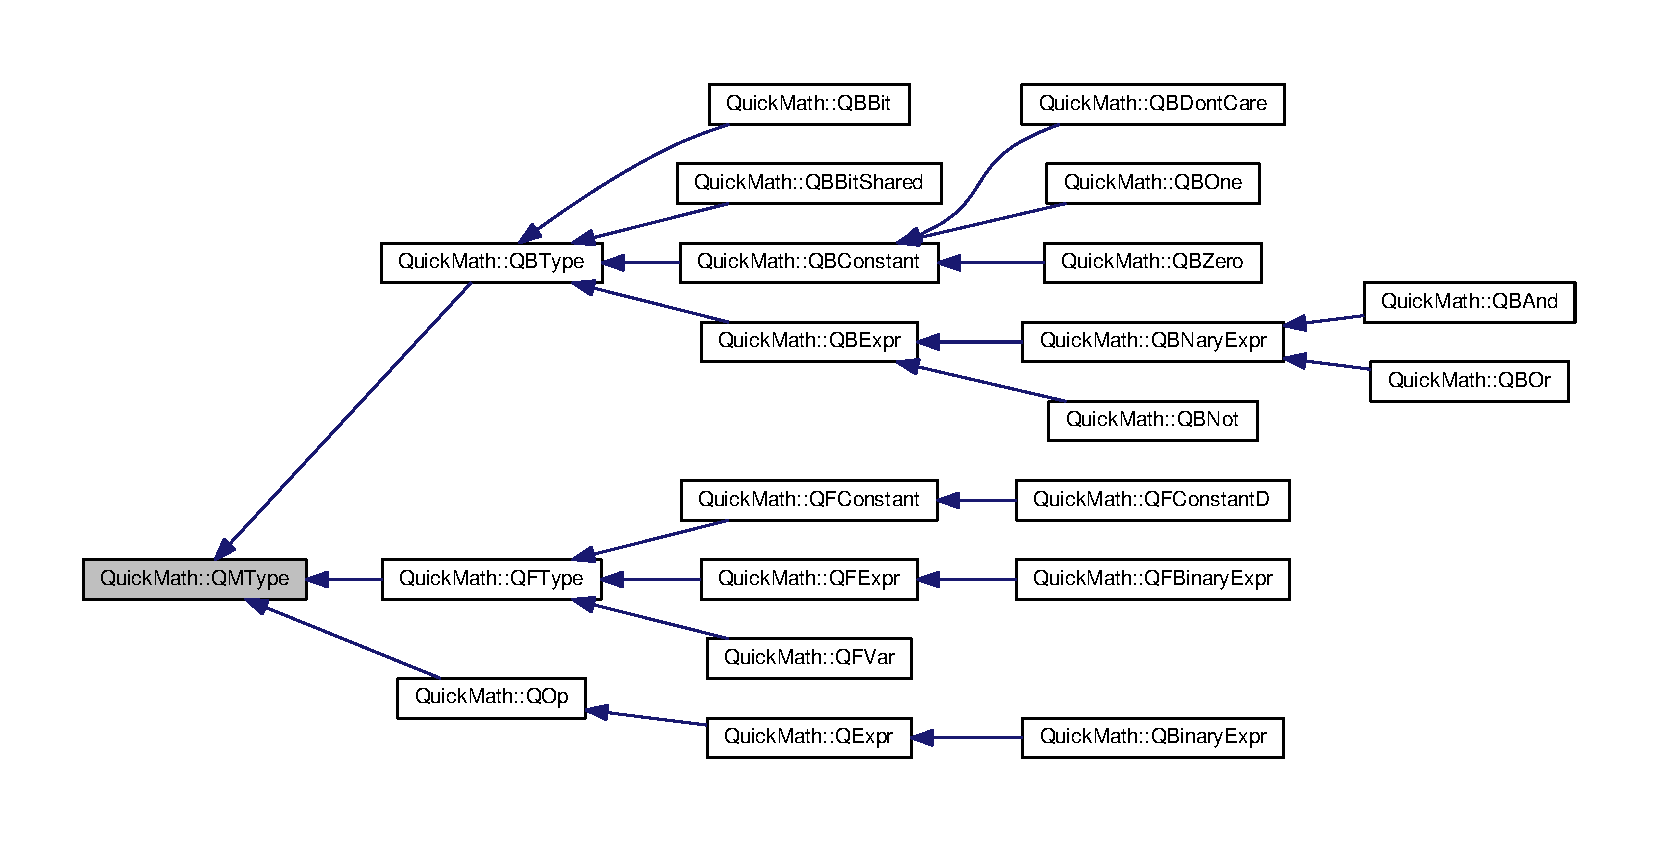
\includegraphics[width=350pt]{classQuickMath_1_1QMType__inherit__graph}
\end{center}
\end{figure}
\subsection*{Public Member Functions}
\begin{DoxyCompactItemize}
\item 
virtual std\+::string \hyperlink{classQuickMath_1_1QMType_a031b83c87e4edae28c65adf8e268442b}{to\+String} () const =0
\item 
virtual bool \hyperlink{classQuickMath_1_1QMType_acb5baa3c93ea3cc6a25c358139b45dd5}{is\+Bool\+Type} () const 
\item 
virtual bool \hyperlink{classQuickMath_1_1QMType_ae9dc3e4b23d53df761e17625688ae404}{is\+Func\+Type} () const 
\item 
virtual bool \hyperlink{classQuickMath_1_1QMType_a79c2716bf5a6b20b9a5bcece2552300b}{is\+Mixed\+Type} () const 
\item 
virtual std\+::unique\+\_\+ptr$<$ \hyperlink{classQuickMath_1_1QMType}{Q\+M\+Type} $>$ \hyperlink{classQuickMath_1_1QMType_a15b2a74a662417da99c6da9b7aaeff77}{clone} () const =0
\end{DoxyCompactItemize}
\subsection*{Friends}
\begin{DoxyCompactItemize}
\item 
std\+::ostream \& \hyperlink{classQuickMath_1_1QMType_ac7f71f6925606054af26eb0e0f98a4a7}{operator$<$$<$} (std\+::ostream \&out\+Stream, const \hyperlink{classQuickMath_1_1QMType}{Q\+M\+Type} \&val)
\end{DoxyCompactItemize}


\subsection{Member Function Documentation}
\hypertarget{classQuickMath_1_1QMType_a15b2a74a662417da99c6da9b7aaeff77}{}\index{Quick\+Math\+::\+Q\+M\+Type@{Quick\+Math\+::\+Q\+M\+Type}!clone@{clone}}
\index{clone@{clone}!Quick\+Math\+::\+Q\+M\+Type@{Quick\+Math\+::\+Q\+M\+Type}}
\subsubsection[{clone}]{\setlength{\rightskip}{0pt plus 5cm}virtual std\+::unique\+\_\+ptr$<${\bf Q\+M\+Type}$>$ Quick\+Math\+::\+Q\+M\+Type\+::clone (
\begin{DoxyParamCaption}
{}
\end{DoxyParamCaption}
) const\hspace{0.3cm}{\ttfamily [pure virtual]}}\label{classQuickMath_1_1QMType_a15b2a74a662417da99c6da9b7aaeff77}


Implemented in \hyperlink{classQuickMath_1_1QBDontCare_a9faa0a15db6993b62efe04632dee9534}{Quick\+Math\+::\+Q\+B\+Dont\+Care}, \hyperlink{classQuickMath_1_1QBBit_a5104a43946ee33625bc7b7ad02850d7a}{Quick\+Math\+::\+Q\+B\+Bit}, \hyperlink{classQuickMath_1_1QBZero_ab2bff50f0df2163ffff4cc07d207df1e}{Quick\+Math\+::\+Q\+B\+Zero}, \hyperlink{classQuickMath_1_1QBOne_ad6247a6496a23cc7025434149d7116fd}{Quick\+Math\+::\+Q\+B\+One}, \hyperlink{classQuickMath_1_1QBinaryExpr_a1a13bf258ab921b56b63914b40a07909}{Quick\+Math\+::\+Q\+Binary\+Expr}, \hyperlink{classQuickMath_1_1QFBinaryExpr_a7f49aef7dd9b8b4c144bbf30395d9051}{Quick\+Math\+::\+Q\+F\+Binary\+Expr}, \hyperlink{classQuickMath_1_1QBBitShared_a8664352f6b5fa48070ffc4fa237a394e}{Quick\+Math\+::\+Q\+B\+Bit\+Shared}, \hyperlink{classQuickMath_1_1QBAnd_a2a2957570e1b333c6190ecf1526c3124}{Quick\+Math\+::\+Q\+B\+And}, \hyperlink{classQuickMath_1_1QBOr_af1ef65aaf163785db31aefa43253cb6c}{Quick\+Math\+::\+Q\+B\+Or}, \hyperlink{classQuickMath_1_1QFVar_a07f3155c995f0cd7dfee1dca2c8ca4d6}{Quick\+Math\+::\+Q\+F\+Var}, \hyperlink{classQuickMath_1_1QBNot_a89d67da57ae064f7ca0f38be07acce50}{Quick\+Math\+::\+Q\+B\+Not}, and \hyperlink{classQuickMath_1_1QFConstantD_ae169fdb14208a3edb0d736051d9e096c}{Quick\+Math\+::\+Q\+F\+Constant\+D}.

\hypertarget{classQuickMath_1_1QMType_acb5baa3c93ea3cc6a25c358139b45dd5}{}\index{Quick\+Math\+::\+Q\+M\+Type@{Quick\+Math\+::\+Q\+M\+Type}!is\+Bool\+Type@{is\+Bool\+Type}}
\index{is\+Bool\+Type@{is\+Bool\+Type}!Quick\+Math\+::\+Q\+M\+Type@{Quick\+Math\+::\+Q\+M\+Type}}
\subsubsection[{is\+Bool\+Type}]{\setlength{\rightskip}{0pt plus 5cm}bool Quick\+Math\+::\+Q\+M\+Type\+::is\+Bool\+Type (
\begin{DoxyParamCaption}
{}
\end{DoxyParamCaption}
) const\hspace{0.3cm}{\ttfamily [virtual]}}\label{classQuickMath_1_1QMType_acb5baa3c93ea3cc6a25c358139b45dd5}


Reimplemented in \hyperlink{classQuickMath_1_1QBType_a9d80f09c8d35de02d0cbb9317d1d326d}{Quick\+Math\+::\+Q\+B\+Type}.

\hypertarget{classQuickMath_1_1QMType_ae9dc3e4b23d53df761e17625688ae404}{}\index{Quick\+Math\+::\+Q\+M\+Type@{Quick\+Math\+::\+Q\+M\+Type}!is\+Func\+Type@{is\+Func\+Type}}
\index{is\+Func\+Type@{is\+Func\+Type}!Quick\+Math\+::\+Q\+M\+Type@{Quick\+Math\+::\+Q\+M\+Type}}
\subsubsection[{is\+Func\+Type}]{\setlength{\rightskip}{0pt plus 5cm}bool Quick\+Math\+::\+Q\+M\+Type\+::is\+Func\+Type (
\begin{DoxyParamCaption}
{}
\end{DoxyParamCaption}
) const\hspace{0.3cm}{\ttfamily [virtual]}}\label{classQuickMath_1_1QMType_ae9dc3e4b23d53df761e17625688ae404}


Reimplemented in \hyperlink{classQuickMath_1_1QFType_a827446c95b66123a6f6cb31087b71ffd}{Quick\+Math\+::\+Q\+F\+Type}.

\hypertarget{classQuickMath_1_1QMType_a79c2716bf5a6b20b9a5bcece2552300b}{}\index{Quick\+Math\+::\+Q\+M\+Type@{Quick\+Math\+::\+Q\+M\+Type}!is\+Mixed\+Type@{is\+Mixed\+Type}}
\index{is\+Mixed\+Type@{is\+Mixed\+Type}!Quick\+Math\+::\+Q\+M\+Type@{Quick\+Math\+::\+Q\+M\+Type}}
\subsubsection[{is\+Mixed\+Type}]{\setlength{\rightskip}{0pt plus 5cm}bool Quick\+Math\+::\+Q\+M\+Type\+::is\+Mixed\+Type (
\begin{DoxyParamCaption}
{}
\end{DoxyParamCaption}
) const\hspace{0.3cm}{\ttfamily [virtual]}}\label{classQuickMath_1_1QMType_a79c2716bf5a6b20b9a5bcece2552300b}


Reimplemented in \hyperlink{classQuickMath_1_1QOp_adc670ad43d65a9dc0239bef089a975e7}{Quick\+Math\+::\+Q\+Op}.

\hypertarget{classQuickMath_1_1QMType_a031b83c87e4edae28c65adf8e268442b}{}\index{Quick\+Math\+::\+Q\+M\+Type@{Quick\+Math\+::\+Q\+M\+Type}!to\+String@{to\+String}}
\index{to\+String@{to\+String}!Quick\+Math\+::\+Q\+M\+Type@{Quick\+Math\+::\+Q\+M\+Type}}
\subsubsection[{to\+String}]{\setlength{\rightskip}{0pt plus 5cm}virtual std\+::string Quick\+Math\+::\+Q\+M\+Type\+::to\+String (
\begin{DoxyParamCaption}
{}
\end{DoxyParamCaption}
) const\hspace{0.3cm}{\ttfamily [pure virtual]}}\label{classQuickMath_1_1QMType_a031b83c87e4edae28c65adf8e268442b}


Implemented in \hyperlink{classQuickMath_1_1QBBit_acf69bfd78922571f1f0ac146c4eed56f}{Quick\+Math\+::\+Q\+B\+Bit}, \hyperlink{classQuickMath_1_1QBinaryExpr_ac253a522b55817ceeff36229d976dc79}{Quick\+Math\+::\+Q\+Binary\+Expr}, \hyperlink{classQuickMath_1_1QFBinaryExpr_a676c949b30d14f919dcdf20151a5b3fe}{Quick\+Math\+::\+Q\+F\+Binary\+Expr}, \hyperlink{classQuickMath_1_1QFVar_a13ed0152f1920b3d7b0f4c86b64d0333}{Quick\+Math\+::\+Q\+F\+Var}, \hyperlink{classQuickMath_1_1QBAnd_abf6c063e663077fdddc4aae96bfbca27}{Quick\+Math\+::\+Q\+B\+And}, \hyperlink{classQuickMath_1_1QBOr_ae835a7fda64bca20388ff3a869a9c928}{Quick\+Math\+::\+Q\+B\+Or}, \hyperlink{classQuickMath_1_1QBBitShared_ab1b3be4ae9548eac373e17038393f8a5}{Quick\+Math\+::\+Q\+B\+Bit\+Shared}, \hyperlink{classQuickMath_1_1QBConstant_a4e277add258b38b9f43da6dde48cd468}{Quick\+Math\+::\+Q\+B\+Constant}, \hyperlink{classQuickMath_1_1QBNot_a946bcf1c86e2f59ea99537cb0fce2a80}{Quick\+Math\+::\+Q\+B\+Not}, \hyperlink{classQuickMath_1_1QFConstantD_a355ad05761ac9e917517eeb9762bceab}{Quick\+Math\+::\+Q\+F\+Constant\+D}, and \hyperlink{classQuickMath_1_1QBType_a12a08061a73649a9f79995469f8297d2}{Quick\+Math\+::\+Q\+B\+Type}.



\subsection{Friends And Related Function Documentation}
\hypertarget{classQuickMath_1_1QMType_ac7f71f6925606054af26eb0e0f98a4a7}{}\index{Quick\+Math\+::\+Q\+M\+Type@{Quick\+Math\+::\+Q\+M\+Type}!operator$<$$<$@{operator$<$$<$}}
\index{operator$<$$<$@{operator$<$$<$}!Quick\+Math\+::\+Q\+M\+Type@{Quick\+Math\+::\+Q\+M\+Type}}
\subsubsection[{operator$<$$<$}]{\setlength{\rightskip}{0pt plus 5cm}std\+::ostream\& operator$<$$<$ (
\begin{DoxyParamCaption}
\item[{std\+::ostream \&}]{out\+Stream, }
\item[{const {\bf Q\+M\+Type} \&}]{val}
\end{DoxyParamCaption}
)\hspace{0.3cm}{\ttfamily [friend]}}\label{classQuickMath_1_1QMType_ac7f71f6925606054af26eb0e0f98a4a7}


The documentation for this class was generated from the following files\+:\begin{DoxyCompactItemize}
\item 
include/\hyperlink{QMType_8h}{Q\+M\+Type.\+h}\item 
src/\hyperlink{QMType_8cpp}{Q\+M\+Type.\+cpp}\end{DoxyCompactItemize}

\hypertarget{classQuickMath_1_1QOp}{}\section{Quick\+Math\+:\+:Q\+Op Class Reference}
\label{classQuickMath_1_1QOp}\index{Quick\+Math\+::\+Q\+Op@{Quick\+Math\+::\+Q\+Op}}


{\ttfamily \#include $<$Q\+Op.\+h$>$}



Inheritance diagram for Quick\+Math\+:\+:Q\+Op\+:
\nopagebreak
\begin{figure}[H]
\begin{center}
\leavevmode
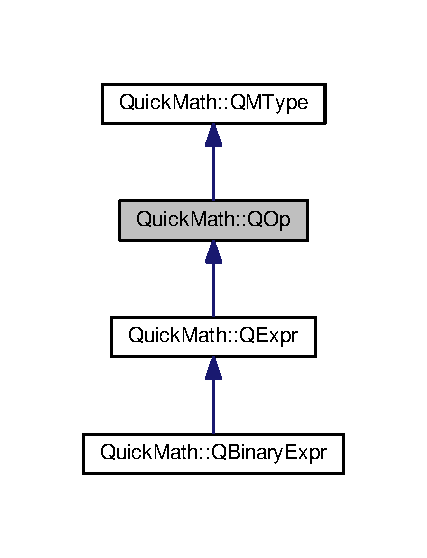
\includegraphics[width=205pt]{classQuickMath_1_1QOp__inherit__graph}
\end{center}
\end{figure}


Collaboration diagram for Quick\+Math\+:\+:Q\+Op\+:
\nopagebreak
\begin{figure}[H]
\begin{center}
\leavevmode
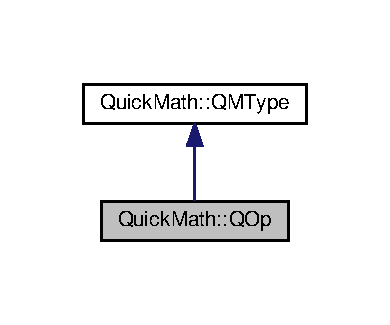
\includegraphics[width=187pt]{classQuickMath_1_1QOp__coll__graph}
\end{center}
\end{figure}
\subsection*{Public Member Functions}
\begin{DoxyCompactItemize}
\item 
bool \hyperlink{classQuickMath_1_1QOp_adc670ad43d65a9dc0239bef089a975e7}{is\+Mixed\+Type} () const 
\end{DoxyCompactItemize}


\subsection{Member Function Documentation}
\hypertarget{classQuickMath_1_1QOp_adc670ad43d65a9dc0239bef089a975e7}{}\index{Quick\+Math\+::\+Q\+Op@{Quick\+Math\+::\+Q\+Op}!is\+Mixed\+Type@{is\+Mixed\+Type}}
\index{is\+Mixed\+Type@{is\+Mixed\+Type}!Quick\+Math\+::\+Q\+Op@{Quick\+Math\+::\+Q\+Op}}
\subsubsection[{is\+Mixed\+Type}]{\setlength{\rightskip}{0pt plus 5cm}bool Quick\+Math\+::\+Q\+Op\+::is\+Mixed\+Type (
\begin{DoxyParamCaption}
{}
\end{DoxyParamCaption}
) const\hspace{0.3cm}{\ttfamily [virtual]}}\label{classQuickMath_1_1QOp_adc670ad43d65a9dc0239bef089a975e7}


Reimplemented from \hyperlink{classQuickMath_1_1QMType_a79c2716bf5a6b20b9a5bcece2552300b}{Quick\+Math\+::\+Q\+M\+Type}.



The documentation for this class was generated from the following files\+:\begin{DoxyCompactItemize}
\item 
include/\+Q\+Mix/\hyperlink{QOp_8h}{Q\+Op.\+h}\item 
src/\+Q\+Mix/\hyperlink{QOp_8cpp}{Q\+Op.\+cpp}\end{DoxyCompactItemize}

\chapter{File Documentation}
\hypertarget{QBAlgorithms_8h}{}\section{include/\+Q\+Bool/\+Q\+B\+Algorithms.h File Reference}
\label{QBAlgorithms_8h}\index{include/\+Q\+Bool/\+Q\+B\+Algorithms.\+h@{include/\+Q\+Bool/\+Q\+B\+Algorithms.\+h}}
{\ttfamily \#include \char`\"{}./\+Q\+B\+Func.\+h\char`\"{}}\\*
{\ttfamily \#include \char`\"{}./\+Q\+B\+Expr.\+h\char`\"{}}\\*
{\ttfamily \#include $<$functional$>$}\\*
Include dependency graph for Q\+B\+Algorithms.\+h\+:
\nopagebreak
\begin{figure}[H]
\begin{center}
\leavevmode
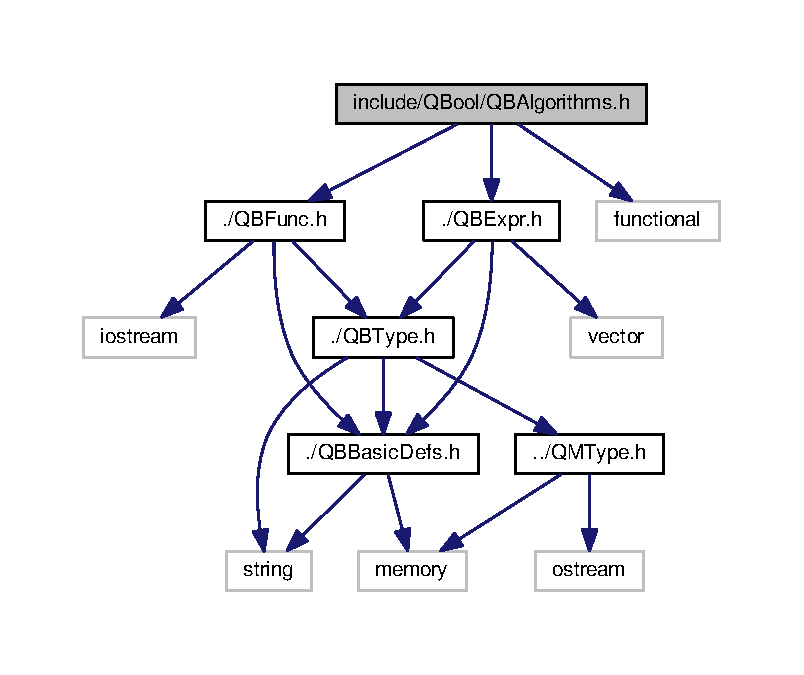
\includegraphics[width=350pt]{QBAlgorithms_8h__incl}
\end{center}
\end{figure}
This graph shows which files directly or indirectly include this file\+:
\nopagebreak
\begin{figure}[H]
\begin{center}
\leavevmode
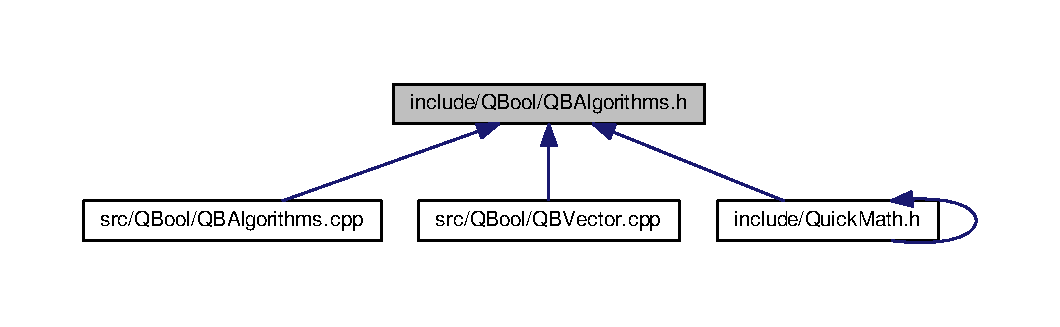
\includegraphics[width=350pt]{QBAlgorithms_8h__dep__incl}
\end{center}
\end{figure}
\subsection*{Namespaces}
\begin{DoxyCompactItemize}
\item 
 \hyperlink{namespaceQuickMath}{Quick\+Math}
\item 
 \hyperlink{namespaceQuickMath_1_1QBAlgo}{Quick\+Math\+::\+Q\+B\+Algo}
\end{DoxyCompactItemize}
\subsection*{Functions}
\begin{DoxyCompactItemize}
\item 
{\footnotesize template$<$typename B\+Func , typename Func $>$ }\\bool \hyperlink{namespaceQuickMath_1_1QBAlgo_ac6ae2b1697b8dd4baa5c903589d1c4e9}{Quick\+Math\+::\+Q\+B\+Algo\+::depth\+Recur} (B\+Func $\ast$expr, Func func)
\item 
{\footnotesize template$<$typename B\+Func , typename Func $>$ }\\void \hyperlink{namespaceQuickMath_1_1QBAlgo_a6ae30dac4638703751de7a5d042d9cb9}{Quick\+Math\+::\+Q\+B\+Algo\+::depth\+Traversal} (B\+Func \&expr, Func func)
\item 
{\footnotesize template$<$typename Func $>$ }\\void \hyperlink{namespaceQuickMath_1_1QBAlgo_a60bdbfc65190e2ac43e3abcf25ffa400}{Quick\+Math\+::\+Q\+B\+Algo\+::depth\+Traversal} (Q\+B\+Type \&expr, Func func)
\item 
Q\+B\+Func \hyperlink{namespaceQuickMath_1_1QBAlgo_a35cc2f24230d4675bebd97ba11aaf47e}{Quick\+Math\+::\+Q\+B\+Algo\+::generate\+C\+N\+F} (const Q\+B\+Func \&func, std\+::string prefix, Q\+B\+Manager \&b\+Man)
\item 
bool \hyperlink{namespaceQuickMath_1_1QBAlgo_af121334ad0919ef45bf1fb0b87f1d31b}{Quick\+Math\+::\+Q\+B\+Algo\+::is\+C\+N\+F} (const Q\+B\+Func \&func)
\item 
vector$<$ Q\+B\+Func $>$ \hyperlink{namespaceQuickMath_1_1QBAlgo_a3cffa5407d5ed739d8d3f1d0763a52a7}{Quick\+Math\+::\+Q\+B\+Algo\+::is\+Sat} (const Q\+B\+Func \&func)
\end{DoxyCompactItemize}

\hypertarget{QBAnd_8h}{}\section{include/\+Q\+Bool/\+Q\+B\+And.h File Reference}
\label{QBAnd_8h}\index{include/\+Q\+Bool/\+Q\+B\+And.\+h@{include/\+Q\+Bool/\+Q\+B\+And.\+h}}
{\ttfamily \#include \char`\"{}./\+Q\+B\+Nary\+Expr.\+h\char`\"{}}\\*
Include dependency graph for Q\+B\+And.\+h\+:
\nopagebreak
\begin{figure}[H]
\begin{center}
\leavevmode
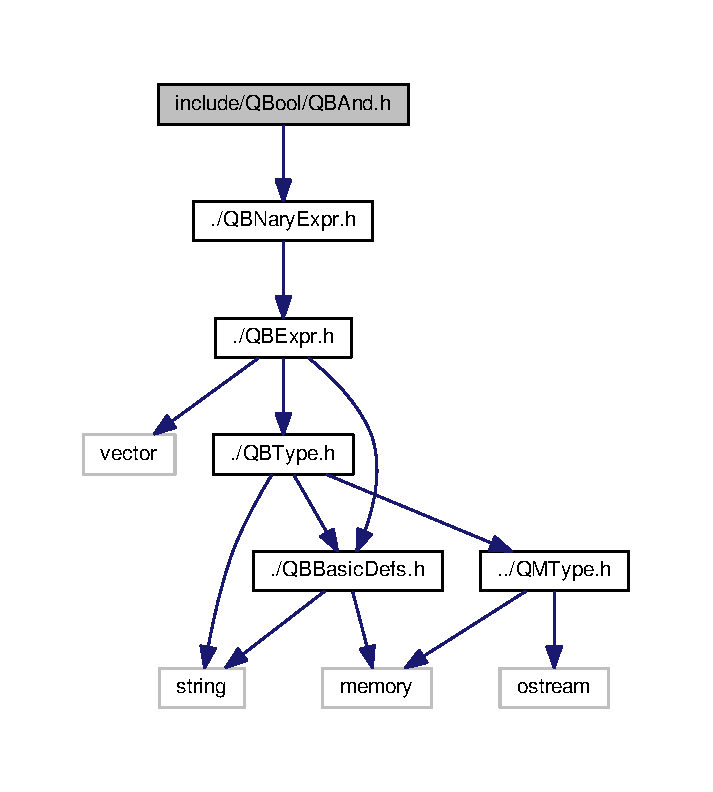
\includegraphics[width=342pt]{QBAnd_8h__incl}
\end{center}
\end{figure}
This graph shows which files directly or indirectly include this file\+:
\nopagebreak
\begin{figure}[H]
\begin{center}
\leavevmode
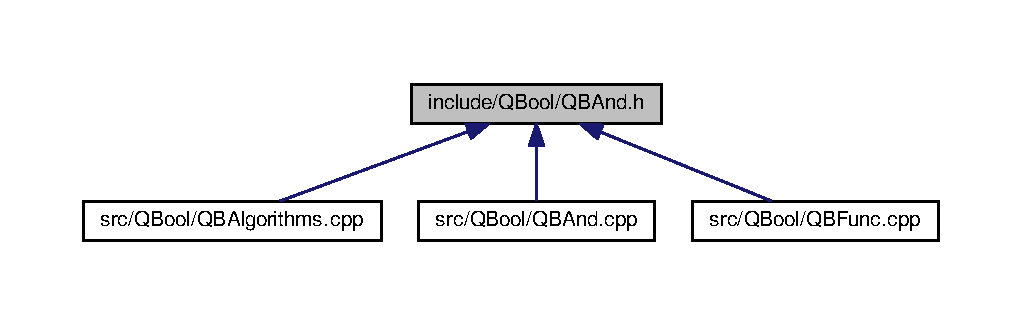
\includegraphics[width=350pt]{QBAnd_8h__dep__incl}
\end{center}
\end{figure}
\subsection*{Classes}
\begin{DoxyCompactItemize}
\item 
class \hyperlink{classQuickMath_1_1QBAnd}{Quick\+Math\+::\+Q\+B\+And}
\end{DoxyCompactItemize}
\subsection*{Namespaces}
\begin{DoxyCompactItemize}
\item 
 \hyperlink{namespaceQuickMath}{Quick\+Math}
\end{DoxyCompactItemize}

\hypertarget{QBBasicDefs_8h}{}\section{include/\+Q\+Bool/\+Q\+B\+Basic\+Defs.h File Reference}
\label{QBBasicDefs_8h}\index{include/\+Q\+Bool/\+Q\+B\+Basic\+Defs.\+h@{include/\+Q\+Bool/\+Q\+B\+Basic\+Defs.\+h}}
{\ttfamily \#include $<$string$>$}\\*
{\ttfamily \#include $<$memory$>$}\\*
Include dependency graph for Q\+B\+Basic\+Defs.\+h\+:
\nopagebreak
\begin{figure}[H]
\begin{center}
\leavevmode
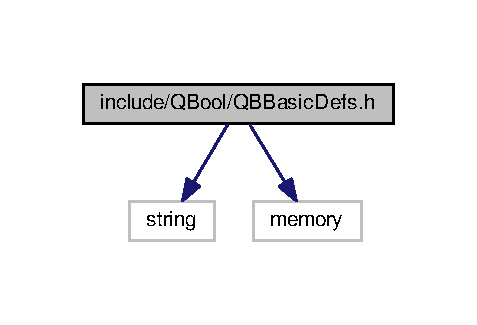
\includegraphics[width=229pt]{QBBasicDefs_8h__incl}
\end{center}
\end{figure}
This graph shows which files directly or indirectly include this file\+:
\nopagebreak
\begin{figure}[H]
\begin{center}
\leavevmode
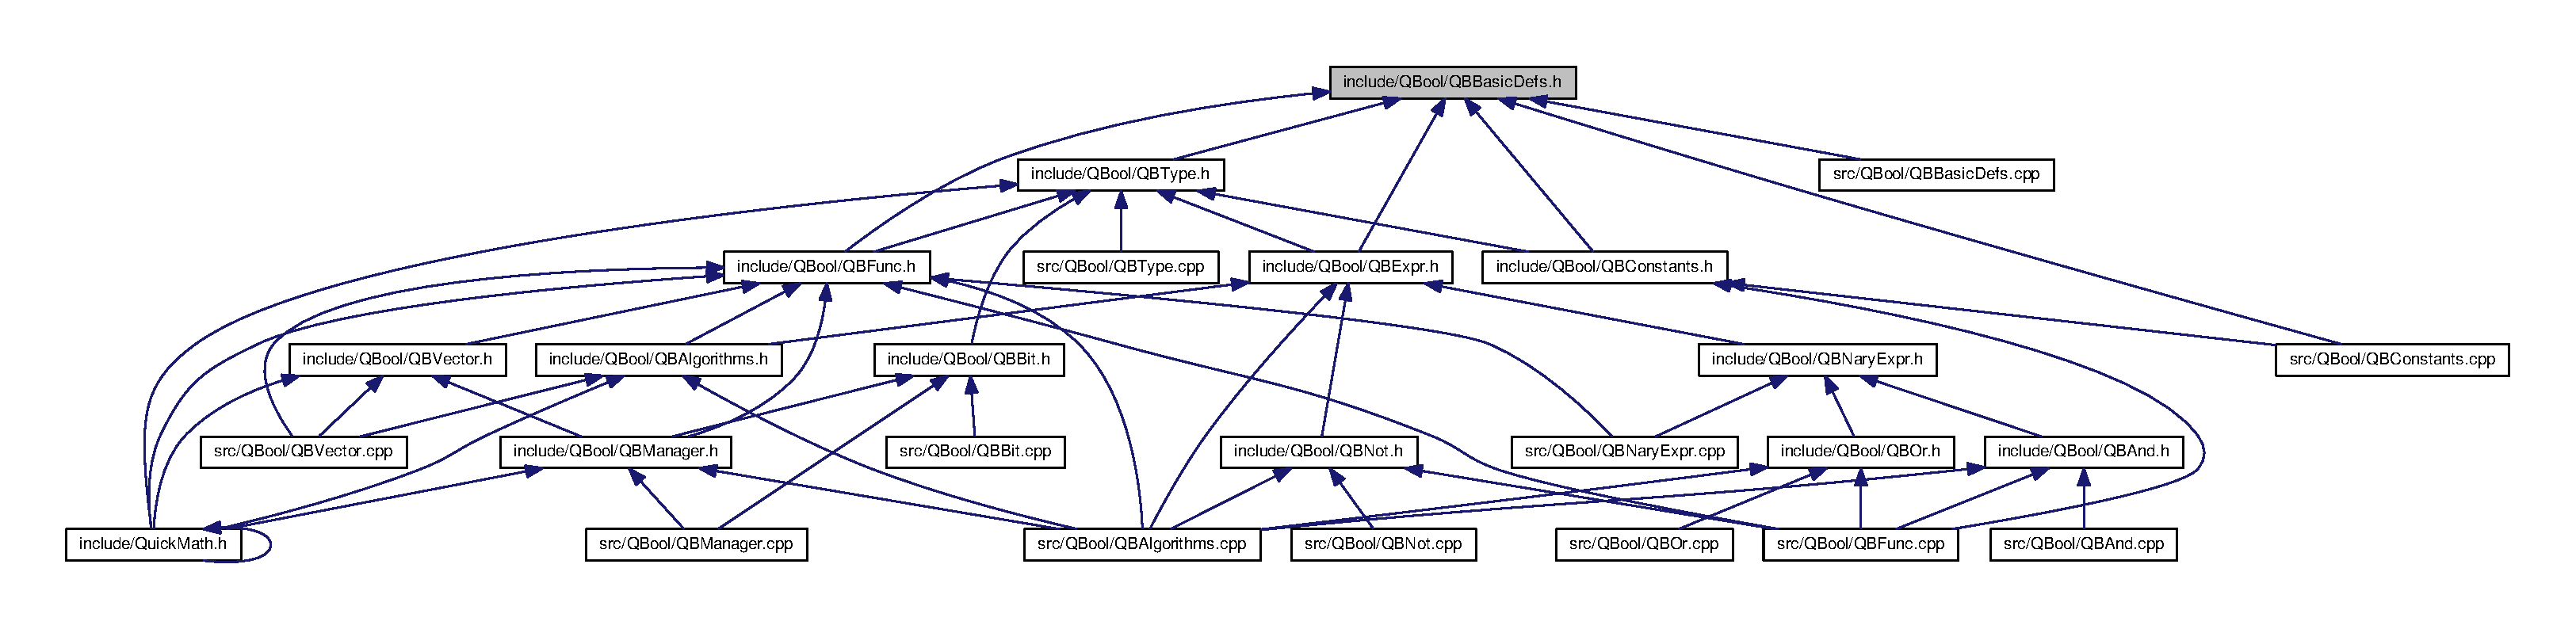
\includegraphics[width=350pt]{QBBasicDefs_8h__dep__incl}
\end{center}
\end{figure}
\subsection*{Namespaces}
\begin{DoxyCompactItemize}
\item 
 \hyperlink{namespaceQuickMath}{Quick\+Math}
\end{DoxyCompactItemize}
\subsection*{Typedefs}
\begin{DoxyCompactItemize}
\item 
typedef std\+::shared\+\_\+ptr$<$ Q\+B\+Type $>$ \hyperlink{namespaceQuickMath_ac7fba3fe1fa7904fe139bbe68de92923}{Quick\+Math\+::\+S\+Q\+B\+Type}
\item 
typedef std\+::unique\+\_\+ptr$<$ Q\+B\+Type $>$ \hyperlink{namespaceQuickMath_af54af2708effd817452548da857ba076}{Quick\+Math\+::\+U\+Q\+B\+Type}
\item 
typedef std\+::shared\+\_\+ptr$<$ Q\+B\+Bit $>$ \hyperlink{namespaceQuickMath_a9d86d757cbfdd10689287a8f6d3f3b99}{Quick\+Math\+::\+S\+Q\+B\+Bit}
\item 
typedef std\+::unique\+\_\+ptr$<$ Q\+B\+Bit $>$ \hyperlink{namespaceQuickMath_a8bf3ddd5067daacf7c170b07a2fe79a1}{Quick\+Math\+::\+U\+Q\+B\+Bit}
\end{DoxyCompactItemize}
\subsection*{Enumerations}
\begin{DoxyCompactItemize}
\item 
enum \hyperlink{namespaceQuickMath_aec13b08c42d9f8e688241623c8b379a0}{Quick\+Math\+::\+Q\+B\+Value} \{ \hyperlink{namespaceQuickMath_aec13b08c42d9f8e688241623c8b379a0a88183b946cc5f0e8c96b2e66e1c74a7e}{Quick\+Math\+::\+Q\+B\+Value\+::\+Unknown}, 
\hyperlink{namespaceQuickMath_aec13b08c42d9f8e688241623c8b379a0a06c2cea18679d64399783748fa367bdd}{Quick\+Math\+::\+Q\+B\+Value\+::\+One}, 
\hyperlink{namespaceQuickMath_aec13b08c42d9f8e688241623c8b379a0ad7ed4ee1df437474d005188535f74875}{Quick\+Math\+::\+Q\+B\+Value\+::\+Zero}, 
\hyperlink{namespaceQuickMath_aec13b08c42d9f8e688241623c8b379a0a60a3629ef6a8f991f45d7a85f2458544}{Quick\+Math\+::\+Q\+B\+Value\+::\+Dont\+Care}
 \}
\end{DoxyCompactItemize}
\subsection*{Functions}
\begin{DoxyCompactItemize}
\item 
std\+::string \hyperlink{namespaceQuickMath_adcde5647f1e74097d4cc15106b49c97f}{Quick\+Math\+::to\+\_\+string} (const Q\+B\+Value \&value)
\end{DoxyCompactItemize}

\hypertarget{QBBit_8h}{}\section{include/\+Q\+Bool/\+Q\+B\+Bit.h File Reference}
\label{QBBit_8h}\index{include/\+Q\+Bool/\+Q\+B\+Bit.\+h@{include/\+Q\+Bool/\+Q\+B\+Bit.\+h}}
{\ttfamily \#include $<$string$>$}\\*
{\ttfamily \#include \char`\"{}./\+Q\+B\+Type.\+h\char`\"{}}\\*
Include dependency graph for Q\+B\+Bit.\+h\+:
\nopagebreak
\begin{figure}[H]
\begin{center}
\leavevmode
\includegraphics[width=341pt]{QBBit_8h__incl}
\end{center}
\end{figure}
This graph shows which files directly or indirectly include this file\+:
\nopagebreak
\begin{figure}[H]
\begin{center}
\leavevmode
\includegraphics[width=350pt]{QBBit_8h__dep__incl}
\end{center}
\end{figure}
\subsection*{Classes}
\begin{DoxyCompactItemize}
\item 
class \hyperlink{classQuickMath_1_1QBBitShared}{Quick\+Math\+::\+Q\+B\+Bit\+Shared}
\item 
class \hyperlink{classQuickMath_1_1QBBit}{Quick\+Math\+::\+Q\+B\+Bit}
\end{DoxyCompactItemize}
\subsection*{Namespaces}
\begin{DoxyCompactItemize}
\item 
 \hyperlink{namespaceQuickMath}{Quick\+Math}
\end{DoxyCompactItemize}

\hypertarget{QBConstants_8h}{}\section{include/\+Q\+Bool/\+Q\+B\+Constants.h File Reference}
\label{QBConstants_8h}\index{include/\+Q\+Bool/\+Q\+B\+Constants.\+h@{include/\+Q\+Bool/\+Q\+B\+Constants.\+h}}
{\ttfamily \#include $<$string$>$}\\*
{\ttfamily \#include \char`\"{}./\+Q\+B\+Basic\+Defs.\+h\char`\"{}}\\*
{\ttfamily \#include \char`\"{}./\+Q\+B\+Type.\+h\char`\"{}}\\*
Include dependency graph for Q\+B\+Constants.\+h\+:
\nopagebreak
\begin{figure}[H]
\begin{center}
\leavevmode
\includegraphics[width=339pt]{QBConstants_8h__incl}
\end{center}
\end{figure}
This graph shows which files directly or indirectly include this file\+:
\nopagebreak
\begin{figure}[H]
\begin{center}
\leavevmode
\includegraphics[width=350pt]{QBConstants_8h__dep__incl}
\end{center}
\end{figure}
\subsection*{Classes}
\begin{DoxyCompactItemize}
\item 
class \hyperlink{classQuickMath_1_1QBConstant}{Quick\+Math\+::\+Q\+B\+Constant}
\item 
class \hyperlink{classQuickMath_1_1QBOne}{Quick\+Math\+::\+Q\+B\+One}
\item 
class \hyperlink{classQuickMath_1_1QBZero}{Quick\+Math\+::\+Q\+B\+Zero}
\item 
class \hyperlink{classQuickMath_1_1QBDontCare}{Quick\+Math\+::\+Q\+B\+Dont\+Care}
\end{DoxyCompactItemize}
\subsection*{Namespaces}
\begin{DoxyCompactItemize}
\item 
 \hyperlink{namespaceQuickMath}{Quick\+Math}
\end{DoxyCompactItemize}

\hypertarget{QBExpr_8h}{}\section{include/\+Q\+Bool/\+Q\+B\+Expr.h File Reference}
\label{QBExpr_8h}\index{include/\+Q\+Bool/\+Q\+B\+Expr.\+h@{include/\+Q\+Bool/\+Q\+B\+Expr.\+h}}
{\ttfamily \#include $<$vector$>$}\\*
{\ttfamily \#include \char`\"{}./\+Q\+B\+Basic\+Defs.\+h\char`\"{}}\\*
{\ttfamily \#include \char`\"{}./\+Q\+B\+Type.\+h\char`\"{}}\\*
Include dependency graph for Q\+B\+Expr.\+h\+:
\nopagebreak
\begin{figure}[H]
\begin{center}
\leavevmode
\includegraphics[width=342pt]{QBExpr_8h__incl}
\end{center}
\end{figure}
This graph shows which files directly or indirectly include this file\+:
\nopagebreak
\begin{figure}[H]
\begin{center}
\leavevmode
\includegraphics[width=350pt]{QBExpr_8h__dep__incl}
\end{center}
\end{figure}
\subsection*{Classes}
\begin{DoxyCompactItemize}
\item 
class \hyperlink{classQuickMath_1_1QBExpr}{Quick\+Math\+::\+Q\+B\+Expr}
\end{DoxyCompactItemize}
\subsection*{Namespaces}
\begin{DoxyCompactItemize}
\item 
 \hyperlink{namespaceQuickMath}{Quick\+Math}
\end{DoxyCompactItemize}

\hypertarget{QBFunc_8h}{}\section{include/\+Q\+Bool/\+Q\+B\+Func.h File Reference}
\label{QBFunc_8h}\index{include/\+Q\+Bool/\+Q\+B\+Func.\+h@{include/\+Q\+Bool/\+Q\+B\+Func.\+h}}
{\ttfamily \#include \char`\"{}./\+Q\+B\+Basic\+Defs.\+h\char`\"{}}\\*
{\ttfamily \#include \char`\"{}./\+Q\+B\+Type.\+h\char`\"{}}\\*
{\ttfamily \#include $<$iostream$>$}\\*
Include dependency graph for Q\+B\+Func.\+h\+:
\nopagebreak
\begin{figure}[H]
\begin{center}
\leavevmode
\includegraphics[width=305pt]{QBFunc_8h__incl}
\end{center}
\end{figure}
This graph shows which files directly or indirectly include this file\+:
\nopagebreak
\begin{figure}[H]
\begin{center}
\leavevmode
\includegraphics[width=350pt]{QBFunc_8h__dep__incl}
\end{center}
\end{figure}
\subsection*{Classes}
\begin{DoxyCompactItemize}
\item 
class \hyperlink{classQuickMath_1_1QBFunc}{Quick\+Math\+::\+Q\+B\+Func}
\end{DoxyCompactItemize}
\subsection*{Namespaces}
\begin{DoxyCompactItemize}
\item 
 \hyperlink{namespaceQuickMath}{Quick\+Math}
\end{DoxyCompactItemize}
\subsection*{Functions}
\begin{DoxyCompactItemize}
\item 
Q\+B\+Func \hyperlink{namespaceQuickMath_a562454d93f506c2c33956c06bce5cf6f}{Quick\+Math\+::bi\+Conditional} (const Q\+B\+Func \&antecedent, const Q\+B\+Func \&consequent)
\item 
Q\+B\+Func \hyperlink{namespaceQuickMath_a8ac0fc1b71f36ab95d586eec93254ba5}{Quick\+Math\+::implication} (const Q\+B\+Func \&antecedent, const Q\+B\+Func \&consequent)
\item 
std\+::ostream \& \hyperlink{namespaceQuickMath_ad40e44735b0edd64ad8308122141be65}{Quick\+Math\+::operator$<$$<$} (std\+::ostream \&stream, const Q\+B\+Func \&func)
\end{DoxyCompactItemize}

\hypertarget{QBManager_8h}{}\section{include/\+Q\+Bool/\+Q\+B\+Manager.h File Reference}
\label{QBManager_8h}\index{include/\+Q\+Bool/\+Q\+B\+Manager.\+h@{include/\+Q\+Bool/\+Q\+B\+Manager.\+h}}
{\ttfamily \#include $<$string$>$}\\*
{\ttfamily \#include $<$map$>$}\\*
{\ttfamily \#include $<$memory$>$}\\*
{\ttfamily \#include \char`\"{}./\+Q\+B\+Func.\+h\char`\"{}}\\*
{\ttfamily \#include \char`\"{}./\+Q\+B\+Vector.\+h\char`\"{}}\\*
{\ttfamily \#include \char`\"{}./\+Q\+B\+Bit.\+h\char`\"{}}\\*
Include dependency graph for Q\+B\+Manager.\+h\+:
\nopagebreak
\begin{figure}[H]
\begin{center}
\leavevmode
\includegraphics[width=350pt]{QBManager_8h__incl}
\end{center}
\end{figure}
This graph shows which files directly or indirectly include this file\+:
\nopagebreak
\begin{figure}[H]
\begin{center}
\leavevmode
\includegraphics[width=350pt]{QBManager_8h__dep__incl}
\end{center}
\end{figure}
\subsection*{Classes}
\begin{DoxyCompactItemize}
\item 
class \hyperlink{classQuickMath_1_1QBManager}{Quick\+Math\+::\+Q\+B\+Manager}
\item 
struct \hyperlink{structQuickMath_1_1QBManager_1_1KeyPair}{Quick\+Math\+::\+Q\+B\+Manager\+::\+Key\+Pair}
\end{DoxyCompactItemize}
\subsection*{Namespaces}
\begin{DoxyCompactItemize}
\item 
 \hyperlink{namespaceQuickMath}{Quick\+Math}
\end{DoxyCompactItemize}

\hypertarget{QBNaryExpr_8h}{}\section{include/\+Q\+Bool/\+Q\+B\+Nary\+Expr.h File Reference}
\label{QBNaryExpr_8h}\index{include/\+Q\+Bool/\+Q\+B\+Nary\+Expr.\+h@{include/\+Q\+Bool/\+Q\+B\+Nary\+Expr.\+h}}
{\ttfamily \#include \char`\"{}./\+Q\+B\+Expr.\+h\char`\"{}}\\*
Include dependency graph for Q\+B\+Nary\+Expr.\+h\+:
\nopagebreak
\begin{figure}[H]
\begin{center}
\leavevmode
\includegraphics[width=342pt]{QBNaryExpr_8h__incl}
\end{center}
\end{figure}
This graph shows which files directly or indirectly include this file\+:
\nopagebreak
\begin{figure}[H]
\begin{center}
\leavevmode
\includegraphics[width=350pt]{QBNaryExpr_8h__dep__incl}
\end{center}
\end{figure}
\subsection*{Classes}
\begin{DoxyCompactItemize}
\item 
class \hyperlink{classQuickMath_1_1QBNaryExpr}{Quick\+Math\+::\+Q\+B\+Nary\+Expr}
\end{DoxyCompactItemize}
\subsection*{Namespaces}
\begin{DoxyCompactItemize}
\item 
 \hyperlink{namespaceQuickMath}{Quick\+Math}
\end{DoxyCompactItemize}

\hypertarget{QBNot_8h}{}\section{include/\+Q\+Bool/\+Q\+B\+Not.h File Reference}
\label{QBNot_8h}\index{include/\+Q\+Bool/\+Q\+B\+Not.\+h@{include/\+Q\+Bool/\+Q\+B\+Not.\+h}}
{\ttfamily \#include \char`\"{}./\+Q\+B\+Expr.\+h\char`\"{}}\\*
Include dependency graph for Q\+B\+Not.\+h\+:
\nopagebreak
\begin{figure}[H]
\begin{center}
\leavevmode
\includegraphics[width=342pt]{QBNot_8h__incl}
\end{center}
\end{figure}
This graph shows which files directly or indirectly include this file\+:
\nopagebreak
\begin{figure}[H]
\begin{center}
\leavevmode
\includegraphics[width=350pt]{QBNot_8h__dep__incl}
\end{center}
\end{figure}
\subsection*{Classes}
\begin{DoxyCompactItemize}
\item 
class \hyperlink{classQuickMath_1_1QBNot}{Quick\+Math\+::\+Q\+B\+Not}
\end{DoxyCompactItemize}
\subsection*{Namespaces}
\begin{DoxyCompactItemize}
\item 
 \hyperlink{namespaceQuickMath}{Quick\+Math}
\end{DoxyCompactItemize}

\hypertarget{QBOr_8h}{}\section{include/\+Q\+Bool/\+Q\+B\+Or.h File Reference}
\label{QBOr_8h}\index{include/\+Q\+Bool/\+Q\+B\+Or.\+h@{include/\+Q\+Bool/\+Q\+B\+Or.\+h}}
{\ttfamily \#include \char`\"{}./\+Q\+B\+Nary\+Expr.\+h\char`\"{}}\\*
Include dependency graph for Q\+B\+Or.\+h\+:
\nopagebreak
\begin{figure}[H]
\begin{center}
\leavevmode
\includegraphics[width=342pt]{QBOr_8h__incl}
\end{center}
\end{figure}
This graph shows which files directly or indirectly include this file\+:
\nopagebreak
\begin{figure}[H]
\begin{center}
\leavevmode
\includegraphics[width=350pt]{QBOr_8h__dep__incl}
\end{center}
\end{figure}
\subsection*{Classes}
\begin{DoxyCompactItemize}
\item 
class \hyperlink{classQuickMath_1_1QBOr}{Quick\+Math\+::\+Q\+B\+Or}
\end{DoxyCompactItemize}
\subsection*{Namespaces}
\begin{DoxyCompactItemize}
\item 
 \hyperlink{namespaceQuickMath}{Quick\+Math}
\end{DoxyCompactItemize}

\hypertarget{QBType_8h}{}\section{include/\+Q\+Bool/\+Q\+B\+Type.h File Reference}
\label{QBType_8h}\index{include/\+Q\+Bool/\+Q\+B\+Type.\+h@{include/\+Q\+Bool/\+Q\+B\+Type.\+h}}
{\ttfamily \#include $<$string$>$}\\*
{\ttfamily \#include \char`\"{}./\+Q\+B\+Basic\+Defs.\+h\char`\"{}}\\*
{\ttfamily \#include \char`\"{}../\+Q\+M\+Type.\+h\char`\"{}}\\*
Include dependency graph for Q\+B\+Type.\+h\+:
\nopagebreak
\begin{figure}[H]
\begin{center}
\leavevmode
\includegraphics[width=305pt]{QBType_8h__incl}
\end{center}
\end{figure}
This graph shows which files directly or indirectly include this file\+:
\nopagebreak
\begin{figure}[H]
\begin{center}
\leavevmode
\includegraphics[width=350pt]{QBType_8h__dep__incl}
\end{center}
\end{figure}
\subsection*{Classes}
\begin{DoxyCompactItemize}
\item 
class \hyperlink{classQuickMath_1_1QBType}{Quick\+Math\+::\+Q\+B\+Type}
\end{DoxyCompactItemize}
\subsection*{Namespaces}
\begin{DoxyCompactItemize}
\item 
 \hyperlink{namespaceQuickMath}{Quick\+Math}
\end{DoxyCompactItemize}

\hypertarget{QBVector_8h}{}\section{include/\+Q\+Bool/\+Q\+B\+Vector.h File Reference}
\label{QBVector_8h}\index{include/\+Q\+Bool/\+Q\+B\+Vector.\+h@{include/\+Q\+Bool/\+Q\+B\+Vector.\+h}}
{\ttfamily \#include $<$vector$>$}\\*
{\ttfamily \#include \char`\"{}./\+Q\+B\+Func.\+h\char`\"{}}\\*
Include dependency graph for Q\+B\+Vector.\+h\+:
\nopagebreak
\begin{figure}[H]
\begin{center}
\leavevmode
\includegraphics[width=305pt]{QBVector_8h__incl}
\end{center}
\end{figure}
This graph shows which files directly or indirectly include this file\+:
\nopagebreak
\begin{figure}[H]
\begin{center}
\leavevmode
\includegraphics[width=350pt]{QBVector_8h__dep__incl}
\end{center}
\end{figure}
\subsection*{Classes}
\begin{DoxyCompactItemize}
\item 
class \hyperlink{classQuickMath_1_1QBVector}{Quick\+Math\+::\+Q\+B\+Vector}
\end{DoxyCompactItemize}
\subsection*{Namespaces}
\begin{DoxyCompactItemize}
\item 
 \hyperlink{namespaceQuickMath}{Quick\+Math}
\end{DoxyCompactItemize}

\hypertarget{QFBinaryExpr_8h}{}\section{include/\+Q\+Func/\+Q\+F\+Binary\+Expr.h File Reference}
\label{QFBinaryExpr_8h}\index{include/\+Q\+Func/\+Q\+F\+Binary\+Expr.\+h@{include/\+Q\+Func/\+Q\+F\+Binary\+Expr.\+h}}
{\ttfamily \#include \char`\"{}./\+Q\+F\+Expr.\+h\char`\"{}}\\*
{\ttfamily \#include $<$array$>$}\\*
{\ttfamily \#include $<$memory$>$}\\*
Include dependency graph for Q\+F\+Binary\+Expr.\+h\+:
\nopagebreak
\begin{figure}[H]
\begin{center}
\leavevmode
\includegraphics[width=350pt]{QFBinaryExpr_8h__incl}
\end{center}
\end{figure}
This graph shows which files directly or indirectly include this file\+:
\nopagebreak
\begin{figure}[H]
\begin{center}
\leavevmode
\includegraphics[width=350pt]{QFBinaryExpr_8h__dep__incl}
\end{center}
\end{figure}
\subsection*{Classes}
\begin{DoxyCompactItemize}
\item 
class \hyperlink{classQuickMath_1_1QFBinaryExpr}{Quick\+Math\+::\+Q\+F\+Binary\+Expr}
\end{DoxyCompactItemize}
\subsection*{Namespaces}
\begin{DoxyCompactItemize}
\item 
 \hyperlink{namespaceQuickMath}{Quick\+Math}
\end{DoxyCompactItemize}

\hypertarget{QFConstant_8h}{}\section{include/\+Q\+Func/\+Q\+F\+Constant.h File Reference}
\label{QFConstant_8h}\index{include/\+Q\+Func/\+Q\+F\+Constant.\+h@{include/\+Q\+Func/\+Q\+F\+Constant.\+h}}
{\ttfamily \#include \char`\"{}./\+Q\+F\+Type.\+h\char`\"{}}\\*
Include dependency graph for Q\+F\+Constant.\+h\+:
\nopagebreak
\begin{figure}[H]
\begin{center}
\leavevmode
\includegraphics[width=250pt]{QFConstant_8h__incl}
\end{center}
\end{figure}
This graph shows which files directly or indirectly include this file\+:
\nopagebreak
\begin{figure}[H]
\begin{center}
\leavevmode
\includegraphics[width=350pt]{QFConstant_8h__dep__incl}
\end{center}
\end{figure}
\subsection*{Classes}
\begin{DoxyCompactItemize}
\item 
class \hyperlink{classQuickMath_1_1QFConstant}{Quick\+Math\+::\+Q\+F\+Constant}
\end{DoxyCompactItemize}
\subsection*{Namespaces}
\begin{DoxyCompactItemize}
\item 
 \hyperlink{namespaceQuickMath}{Quick\+Math}
\end{DoxyCompactItemize}

\hypertarget{QFConstantD_8h}{}\section{include/\+Q\+Func/\+Q\+F\+Constant\+D.h File Reference}
\label{QFConstantD_8h}\index{include/\+Q\+Func/\+Q\+F\+Constant\+D.\+h@{include/\+Q\+Func/\+Q\+F\+Constant\+D.\+h}}
{\ttfamily \#include \char`\"{}./\+Q\+F\+Constant.\+h\char`\"{}}\\*
Include dependency graph for Q\+F\+Constant\+D.\+h\+:
\nopagebreak
\begin{figure}[H]
\begin{center}
\leavevmode
\includegraphics[width=254pt]{QFConstantD_8h__incl}
\end{center}
\end{figure}
This graph shows which files directly or indirectly include this file\+:
\nopagebreak
\begin{figure}[H]
\begin{center}
\leavevmode
\includegraphics[width=350pt]{QFConstantD_8h__dep__incl}
\end{center}
\end{figure}
\subsection*{Classes}
\begin{DoxyCompactItemize}
\item 
class \hyperlink{classQuickMath_1_1QFConstantD}{Quick\+Math\+::\+Q\+F\+Constant\+D}
\end{DoxyCompactItemize}
\subsection*{Namespaces}
\begin{DoxyCompactItemize}
\item 
 \hyperlink{namespaceQuickMath}{Quick\+Math}
\end{DoxyCompactItemize}

\hypertarget{QFExpr_8h}{}\section{include/\+Q\+Func/\+Q\+F\+Expr.h File Reference}
\label{QFExpr_8h}\index{include/\+Q\+Func/\+Q\+F\+Expr.\+h@{include/\+Q\+Func/\+Q\+F\+Expr.\+h}}
{\ttfamily \#include \char`\"{}./\+Q\+F\+Type.\+h\char`\"{}}\\*
{\ttfamily \#include \char`\"{}../\+Q\+M\+Defs.\+h\char`\"{}}\\*
Include dependency graph for Q\+F\+Expr.\+h\+:
\nopagebreak
\begin{figure}[H]
\begin{center}
\leavevmode
\includegraphics[width=277pt]{QFExpr_8h__incl}
\end{center}
\end{figure}
This graph shows which files directly or indirectly include this file\+:
\nopagebreak
\begin{figure}[H]
\begin{center}
\leavevmode
\includegraphics[width=350pt]{QFExpr_8h__dep__incl}
\end{center}
\end{figure}
\subsection*{Classes}
\begin{DoxyCompactItemize}
\item 
class \hyperlink{classQuickMath_1_1QFExpr}{Quick\+Math\+::\+Q\+F\+Expr}
\end{DoxyCompactItemize}
\subsection*{Namespaces}
\begin{DoxyCompactItemize}
\item 
 \hyperlink{namespaceQuickMath}{Quick\+Math}
\end{DoxyCompactItemize}

\hypertarget{QFType_8h}{}\section{include/\+Q\+Func/\+Q\+F\+Type.h File Reference}
\label{QFType_8h}\index{include/\+Q\+Func/\+Q\+F\+Type.\+h@{include/\+Q\+Func/\+Q\+F\+Type.\+h}}
{\ttfamily \#include $<$string$>$}\\*
{\ttfamily \#include \char`\"{}../\+Q\+M\+Type.\+h\char`\"{}}\\*
Include dependency graph for Q\+F\+Type.\+h\+:
\nopagebreak
\begin{figure}[H]
\begin{center}
\leavevmode
\includegraphics[width=241pt]{QFType_8h__incl}
\end{center}
\end{figure}
This graph shows which files directly or indirectly include this file\+:
\nopagebreak
\begin{figure}[H]
\begin{center}
\leavevmode
\includegraphics[width=350pt]{QFType_8h__dep__incl}
\end{center}
\end{figure}
\subsection*{Classes}
\begin{DoxyCompactItemize}
\item 
class \hyperlink{classQuickMath_1_1QFType}{Quick\+Math\+::\+Q\+F\+Type}
\end{DoxyCompactItemize}
\subsection*{Namespaces}
\begin{DoxyCompactItemize}
\item 
 \hyperlink{namespaceQuickMath}{Quick\+Math}
\end{DoxyCompactItemize}

\hypertarget{QFVar_8h}{}\section{include/\+Q\+Func/\+Q\+F\+Var.h File Reference}
\label{QFVar_8h}\index{include/\+Q\+Func/\+Q\+F\+Var.\+h@{include/\+Q\+Func/\+Q\+F\+Var.\+h}}
{\ttfamily \#include \char`\"{}./\+Q\+F\+Type.\+h\char`\"{}}\\*
Include dependency graph for Q\+F\+Var.\+h\+:
\nopagebreak
\begin{figure}[H]
\begin{center}
\leavevmode
\includegraphics[width=238pt]{QFVar_8h__incl}
\end{center}
\end{figure}
This graph shows which files directly or indirectly include this file\+:
\nopagebreak
\begin{figure}[H]
\begin{center}
\leavevmode
\includegraphics[width=336pt]{QFVar_8h__dep__incl}
\end{center}
\end{figure}
\subsection*{Classes}
\begin{DoxyCompactItemize}
\item 
class \hyperlink{classQuickMath_1_1QFVar}{Quick\+Math\+::\+Q\+F\+Var}
\end{DoxyCompactItemize}
\subsection*{Namespaces}
\begin{DoxyCompactItemize}
\item 
 \hyperlink{namespaceQuickMath}{Quick\+Math}
\end{DoxyCompactItemize}

\hypertarget{QMDefs_8h}{}\section{include/\+Q\+M\+Defs.h File Reference}
\label{QMDefs_8h}\index{include/\+Q\+M\+Defs.\+h@{include/\+Q\+M\+Defs.\+h}}
{\ttfamily \#include $<$memory$>$}\\*
Include dependency graph for Q\+M\+Defs.\+h\+:
\nopagebreak
\begin{figure}[H]
\begin{center}
\leavevmode
\includegraphics[width=175pt]{QMDefs_8h__incl}
\end{center}
\end{figure}
This graph shows which files directly or indirectly include this file\+:
\nopagebreak
\begin{figure}[H]
\begin{center}
\leavevmode
\includegraphics[width=350pt]{QMDefs_8h__dep__incl}
\end{center}
\end{figure}
\subsection*{Namespaces}
\begin{DoxyCompactItemize}
\item 
 \hyperlink{namespaceQuickMath}{Quick\+Math}
\end{DoxyCompactItemize}
\subsection*{Enumerations}
\begin{DoxyCompactItemize}
\item 
enum \hyperlink{namespaceQuickMath_a0a6c67b9dab0cfd5f3e711b0573545cb}{Quick\+Math\+::\+Q\+M\+Op\+Type} \{ \\*
\hyperlink{namespaceQuickMath_a0a6c67b9dab0cfd5f3e711b0573545cbac562607189d77eb9dfb707464c1e7b0b}{Quick\+Math\+::\+Q\+M\+Op\+Type\+::\+L\+T}, 
\hyperlink{namespaceQuickMath_a0a6c67b9dab0cfd5f3e711b0573545cbacc981ecc65ecf63ad1673cbec9c64198}{Quick\+Math\+::\+Q\+M\+Op\+Type\+::\+L\+T\+E}, 
\hyperlink{namespaceQuickMath_a0a6c67b9dab0cfd5f3e711b0573545cbacd6a9bd2a175104eed40f0d33a8b4020}{Quick\+Math\+::\+Q\+M\+Op\+Type\+::\+G\+T}, 
\hyperlink{namespaceQuickMath_a0a6c67b9dab0cfd5f3e711b0573545cba32d35312e8f24bc1669bd2b45c00d47c}{Quick\+Math\+::\+Q\+M\+Op\+Type\+::\+G\+T\+E}, 
\\*
\hyperlink{namespaceQuickMath_a0a6c67b9dab0cfd5f3e711b0573545cbadc33066c3993e0d50896e533fd692ce0}{Quick\+Math\+::\+Q\+M\+Op\+Type\+::\+N\+E}, 
\hyperlink{namespaceQuickMath_a0a6c67b9dab0cfd5f3e711b0573545cba2dcbad7477fd40561e8b8198f173bd47}{Quick\+Math\+::\+Q\+M\+Op\+Type\+::\+E\+Q}, 
\hyperlink{namespaceQuickMath_a0a6c67b9dab0cfd5f3e711b0573545cba417054607c4620cb1c90cf0219d82c98}{Quick\+Math\+::\+Q\+M\+Op\+Type\+::\+B\+I\+C\+O\+N\+D}, 
\hyperlink{namespaceQuickMath_a0a6c67b9dab0cfd5f3e711b0573545cba27a9f92549363f04ef46148fe9e87eee}{Quick\+Math\+::\+Q\+M\+Op\+Type\+::\+I\+M\+P\+L}, 
\\*
\hyperlink{namespaceQuickMath_a0a6c67b9dab0cfd5f3e711b0573545cba479a809c0b6eaaefd3b1df16f976df06}{Quick\+Math\+::\+Q\+M\+Op\+Type\+::\+L\+A\+N\+D}, 
\hyperlink{namespaceQuickMath_a0a6c67b9dab0cfd5f3e711b0573545cbad3335c358811cfc353257e21b1d38229}{Quick\+Math\+::\+Q\+M\+Op\+Type\+::\+L\+O\+R}, 
\hyperlink{namespaceQuickMath_a0a6c67b9dab0cfd5f3e711b0573545cba81145009eec44ad2c399c9459a01d8f0}{Quick\+Math\+::\+Q\+M\+Op\+Type\+::\+L\+N\+O\+T}, 
\hyperlink{namespaceQuickMath_a0a6c67b9dab0cfd5f3e711b0573545cbaa8a5bbeedca093b94b7f0d3f185b98f7}{Quick\+Math\+::\+Q\+M\+Op\+Type\+::\+B\+A\+N\+D}, 
\\*
\hyperlink{namespaceQuickMath_a0a6c67b9dab0cfd5f3e711b0573545cba0adf6aac232504c55ea4202e09498bfd}{Quick\+Math\+::\+Q\+M\+Op\+Type\+::\+B\+O\+R}, 
\hyperlink{namespaceQuickMath_a0a6c67b9dab0cfd5f3e711b0573545cba0fd78279a775c262180e0cfbad6fa9eb}{Quick\+Math\+::\+Q\+M\+Op\+Type\+::\+B\+N\+O\+T}, 
\hyperlink{namespaceQuickMath_a0a6c67b9dab0cfd5f3e711b0573545cba40adb8f562959dd6dcfabc212f72a607}{Quick\+Math\+::\+Q\+M\+Op\+Type\+::\+U\+K\+N\+W\+N}
 \}
\end{DoxyCompactItemize}
\subsection*{Functions}
\begin{DoxyCompactItemize}
\item 
{\footnotesize template$<$typename Derived , typename Base $>$ }\\std\+::unique\+\_\+ptr$<$ Derived $>$ \hyperlink{namespaceQuickMath_ae96dd5e8f317ec3047ca4daf0e95c53c}{Quick\+Math\+::static\+\_\+uptr\+\_\+cast} (std\+::unique\+\_\+ptr$<$ Base $>$ \&\&p)
\item 
{\footnotesize template$<$typename Derived , typename Base , typename Del $>$ }\\std\+::unique\+\_\+ptr$<$ Derived, Del $>$ \hyperlink{namespaceQuickMath_afd2de1a5f61fb3f1eba5a9e84117f72a}{Quick\+Math\+::dynamic\+\_\+uptr\+\_\+cast} (std\+::unique\+\_\+ptr$<$ Base, Del $>$ \&\&p)
\end{DoxyCompactItemize}

\hypertarget{QBinaryExpr_8h}{}\section{include/\+Q\+Mix/\+Q\+Binary\+Expr.h File Reference}
\label{QBinaryExpr_8h}\index{include/\+Q\+Mix/\+Q\+Binary\+Expr.\+h@{include/\+Q\+Mix/\+Q\+Binary\+Expr.\+h}}
{\ttfamily \#include $<$memory$>$}\\*
{\ttfamily \#include \char`\"{}./\+Q\+Expr.\+h\char`\"{}}\\*
{\ttfamily \#include \char`\"{}../\+Q\+M\+Defs.\+h\char`\"{}}\\*
Include dependency graph for Q\+Binary\+Expr.\+h\+:
\nopagebreak
\begin{figure}[H]
\begin{center}
\leavevmode
\includegraphics[width=273pt]{QBinaryExpr_8h__incl}
\end{center}
\end{figure}
This graph shows which files directly or indirectly include this file\+:
\nopagebreak
\begin{figure}[H]
\begin{center}
\leavevmode
\includegraphics[width=350pt]{QBinaryExpr_8h__dep__incl}
\end{center}
\end{figure}
\subsection*{Classes}
\begin{DoxyCompactItemize}
\item 
class \hyperlink{classQuickMath_1_1QBinaryExpr}{Quick\+Math\+::\+Q\+Binary\+Expr}
\end{DoxyCompactItemize}
\subsection*{Namespaces}
\begin{DoxyCompactItemize}
\item 
 \hyperlink{namespaceQuickMath}{Quick\+Math}
\end{DoxyCompactItemize}

\hypertarget{QExpr_8h}{}\section{include/\+Q\+Mix/\+Q\+Expr.h File Reference}
\label{QExpr_8h}\index{include/\+Q\+Mix/\+Q\+Expr.\+h@{include/\+Q\+Mix/\+Q\+Expr.\+h}}
{\ttfamily \#include \char`\"{}./\+Q\+Op.\+h\char`\"{}}\\*
{\ttfamily \#include \char`\"{}../\+Q\+M\+Defs.\+h\char`\"{}}\\*
Include dependency graph for Q\+Expr.\+h\+:
\nopagebreak
\begin{figure}[H]
\begin{center}
\leavevmode
\includegraphics[width=240pt]{QExpr_8h__incl}
\end{center}
\end{figure}
This graph shows which files directly or indirectly include this file\+:
\nopagebreak
\begin{figure}[H]
\begin{center}
\leavevmode
\includegraphics[width=350pt]{QExpr_8h__dep__incl}
\end{center}
\end{figure}
\subsection*{Classes}
\begin{DoxyCompactItemize}
\item 
class \hyperlink{classQuickMath_1_1QExpr}{Quick\+Math\+::\+Q\+Expr}
\end{DoxyCompactItemize}
\subsection*{Namespaces}
\begin{DoxyCompactItemize}
\item 
 \hyperlink{namespaceQuickMath}{Quick\+Math}
\end{DoxyCompactItemize}

\hypertarget{QOp_8h}{}\section{include/\+Q\+Mix/\+Q\+Op.h File Reference}
\label{QOp_8h}\index{include/\+Q\+Mix/\+Q\+Op.\+h@{include/\+Q\+Mix/\+Q\+Op.\+h}}
{\ttfamily \#include \char`\"{}../\+Q\+M\+Type.\+h\char`\"{}}\\*
Include dependency graph for Q\+Op.\+h\+:
\nopagebreak
\begin{figure}[H]
\begin{center}
\leavevmode
\includegraphics[width=202pt]{QOp_8h__incl}
\end{center}
\end{figure}
This graph shows which files directly or indirectly include this file\+:
\nopagebreak
\begin{figure}[H]
\begin{center}
\leavevmode
\includegraphics[width=350pt]{QOp_8h__dep__incl}
\end{center}
\end{figure}
\subsection*{Classes}
\begin{DoxyCompactItemize}
\item 
class \hyperlink{classQuickMath_1_1QOp}{Quick\+Math\+::\+Q\+Op}
\end{DoxyCompactItemize}
\subsection*{Namespaces}
\begin{DoxyCompactItemize}
\item 
 \hyperlink{namespaceQuickMath}{Quick\+Math}
\end{DoxyCompactItemize}

\hypertarget{QMType_8h}{}\section{include/\+Q\+M\+Type.h File Reference}
\label{QMType_8h}\index{include/\+Q\+M\+Type.\+h@{include/\+Q\+M\+Type.\+h}}
{\ttfamily \#include $<$ostream$>$}\\*
{\ttfamily \#include $<$memory$>$}\\*
Include dependency graph for Q\+M\+Type.\+h\+:
\nopagebreak
\begin{figure}[H]
\begin{center}
\leavevmode
\includegraphics[width=202pt]{QMType_8h__incl}
\end{center}
\end{figure}
This graph shows which files directly or indirectly include this file\+:
\nopagebreak
\begin{figure}[H]
\begin{center}
\leavevmode
\includegraphics[width=350pt]{QMType_8h__dep__incl}
\end{center}
\end{figure}
\subsection*{Classes}
\begin{DoxyCompactItemize}
\item 
class \hyperlink{classQuickMath_1_1QMType}{Quick\+Math\+::\+Q\+M\+Type}
\end{DoxyCompactItemize}
\subsection*{Namespaces}
\begin{DoxyCompactItemize}
\item 
 \hyperlink{namespaceQuickMath}{Quick\+Math}
\end{DoxyCompactItemize}

\hypertarget{QuickMath_8h}{}\section{include/\+Quick\+Math.h File Reference}
\label{QuickMath_8h}\index{include/\+Quick\+Math.\+h@{include/\+Quick\+Math.\+h}}
{\ttfamily \#include \char`\"{}Quick\+Math.\+h\char`\"{}}\\*
{\ttfamily \#include \char`\"{}Q\+M\+Type.\+h\char`\"{}}\\*
{\ttfamily \#include \char`\"{}Q\+M\+Defs.\+h\char`\"{}}\\*
{\ttfamily \#include \char`\"{}./\+Q\+Mix/\+Q\+Binary\+Expr.\+h\char`\"{}}\\*
{\ttfamily \#include \char`\"{}./\+Q\+Func/\+Q\+F\+Var.\+h\char`\"{}}\\*
{\ttfamily \#include \char`\"{}./\+Q\+Func/\+Q\+F\+Type.\+h\char`\"{}}\\*
{\ttfamily \#include \char`\"{}./\+Q\+Func/\+Q\+F\+Binary\+Expr.\+h\char`\"{}}\\*
{\ttfamily \#include \char`\"{}./\+Q\+Func/\+Q\+F\+Constant\+D.\+h\char`\"{}}\\*
{\ttfamily \#include \char`\"{}./\+Q\+Bool/\+Q\+B\+Func.\+h\char`\"{}}\\*
{\ttfamily \#include \char`\"{}./\+Q\+Bool/\+Q\+B\+Type.\+h\char`\"{}}\\*
{\ttfamily \#include \char`\"{}./\+Q\+Bool/\+Q\+B\+Vector.\+h\char`\"{}}\\*
{\ttfamily \#include \char`\"{}./\+Q\+Bool/\+Q\+B\+Manager.\+h\char`\"{}}\\*
{\ttfamily \#include \char`\"{}./\+Q\+Bool/\+Q\+B\+Algorithms.\+h\char`\"{}}\\*
Include dependency graph for Quick\+Math.\+h\+:
\nopagebreak
\begin{figure}[H]
\begin{center}
\leavevmode
\includegraphics[width=350pt]{QuickMath_8h__incl}
\end{center}
\end{figure}
This graph shows which files directly or indirectly include this file\+:
\nopagebreak
\begin{figure}[H]
\begin{center}
\leavevmode
\includegraphics[width=204pt]{QuickMath_8h__dep__incl}
\end{center}
\end{figure}

\hypertarget{QBAlgorithms_8cpp}{}\section{src/\+Q\+Bool/\+Q\+B\+Algorithms.cpp File Reference}
\label{QBAlgorithms_8cpp}\index{src/\+Q\+Bool/\+Q\+B\+Algorithms.\+cpp@{src/\+Q\+Bool/\+Q\+B\+Algorithms.\+cpp}}
{\ttfamily \#include \char`\"{}Q\+Bool/\+Q\+B\+Algorithms.\+h\char`\"{}}\\*
{\ttfamily \#include \char`\"{}Q\+Bool/\+Q\+B\+Expr.\+h\char`\"{}}\\*
{\ttfamily \#include \char`\"{}Q\+Bool/\+Q\+B\+Manager.\+h\char`\"{}}\\*
{\ttfamily \#include \char`\"{}Q\+Bool/\+Q\+B\+And.\+h\char`\"{}}\\*
{\ttfamily \#include \char`\"{}Q\+Bool/\+Q\+B\+Or.\+h\char`\"{}}\\*
{\ttfamily \#include \char`\"{}Q\+Bool/\+Q\+B\+Not.\+h\char`\"{}}\\*
{\ttfamily \#include \char`\"{}Q\+Bool/\+Q\+B\+Func.\+h\char`\"{}}\\*
{\ttfamily \#include $<$iostream$>$}\\*
{\ttfamily \#include $<$string$>$}\\*
{\ttfamily \#include $<$stack$>$}\\*
{\ttfamily \#include $<$tuple$>$}\\*
{\ttfamily \#include $<$map$>$}\\*
{\ttfamily \#include $<$sstream$>$}\\*
{\ttfamily \#include $<$cassert$>$}\\*
{\ttfamily \#include $<$unistd.\+h$>$}\\*
Include dependency graph for Q\+B\+Algorithms.\+cpp\+:
\nopagebreak
\begin{figure}[H]
\begin{center}
\leavevmode
\includegraphics[width=350pt]{QBAlgorithms_8cpp__incl}
\end{center}
\end{figure}
\subsection*{Classes}
\begin{DoxyCompactItemize}
\item 
struct \hyperlink{structQuickMath_1_1QBAlgo_1_1QBBitCmp}{Quick\+Math\+::\+Q\+B\+Algo\+::\+Q\+B\+Bit\+Cmp}
\end{DoxyCompactItemize}
\subsection*{Namespaces}
\begin{DoxyCompactItemize}
\item 
 \hyperlink{namespaceQuickMath}{Quick\+Math}
\item 
 \hyperlink{namespaceQuickMath_1_1QBAlgo}{Quick\+Math\+::\+Q\+B\+Algo}
\end{DoxyCompactItemize}
\subsection*{Functions}
\begin{DoxyCompactItemize}
\item 
Q\+B\+Func \hyperlink{namespaceQuickMath_1_1QBAlgo_a38967d834625639ad4040038c274f6c4}{Quick\+Math\+::\+Q\+B\+Algo\+::generate\+C\+N\+F} (const Q\+B\+Func \&func, string prefix, Q\+B\+Manager \&b\+Man)
\item 
bool \hyperlink{namespaceQuickMath_1_1QBAlgo_a58928a3d288af7c50e94a63f54b4fd3a}{Quick\+Math\+::\+Q\+B\+Algo\+::is\+C\+N\+F\+Not\+Term} (const Q\+B\+Not $\ast$expr)
\item 
bool \hyperlink{namespaceQuickMath_1_1QBAlgo_ae084c53f5dedaa733811c3563601379b}{Quick\+Math\+::\+Q\+B\+Algo\+::is\+C\+N\+F\+Or\+Term} (const Q\+B\+Or $\ast$expr)
\item 
bool \hyperlink{namespaceQuickMath_1_1QBAlgo_af121334ad0919ef45bf1fb0b87f1d31b}{Quick\+Math\+::\+Q\+B\+Algo\+::is\+C\+N\+F} (const Q\+B\+Func \&func)
\item 
vector$<$ int $>$ \hyperlink{namespaceQuickMath_1_1QBAlgo_aa04e30fe5d4d870de2adb8e01f7e918e}{Quick\+Math\+::\+Q\+B\+Algo\+::run\+Lingeling\+Sat} (std\+::string \&\&dimacs\+Str)
\item 
vector$<$ Q\+B\+Func $>$ \hyperlink{namespaceQuickMath_1_1QBAlgo_a3cffa5407d5ed739d8d3f1d0763a52a7}{Quick\+Math\+::\+Q\+B\+Algo\+::is\+Sat} (const Q\+B\+Func \&func)
\end{DoxyCompactItemize}

\hypertarget{QBAnd_8cpp}{}\section{src/\+Q\+Bool/\+Q\+B\+And.cpp File Reference}
\label{QBAnd_8cpp}\index{src/\+Q\+Bool/\+Q\+B\+And.\+cpp@{src/\+Q\+Bool/\+Q\+B\+And.\+cpp}}
{\ttfamily \#include \char`\"{}Q\+Bool/\+Q\+B\+And.\+h\char`\"{}}\\*
{\ttfamily \#include \char`\"{}Q\+M\+Defs.\+h\char`\"{}}\\*
{\ttfamily \#include $<$iostream$>$}\\*
Include dependency graph for Q\+B\+And.\+cpp\+:
\nopagebreak
\begin{figure}[H]
\begin{center}
\leavevmode
\includegraphics[width=350pt]{QBAnd_8cpp__incl}
\end{center}
\end{figure}
\subsection*{Namespaces}
\begin{DoxyCompactItemize}
\item 
 \hyperlink{namespaceQuickMath}{Quick\+Math}
\end{DoxyCompactItemize}

\hypertarget{QBBasicDefs_8cpp}{}\section{src/\+Q\+Bool/\+Q\+B\+Basic\+Defs.cpp File Reference}
\label{QBBasicDefs_8cpp}\index{src/\+Q\+Bool/\+Q\+B\+Basic\+Defs.\+cpp@{src/\+Q\+Bool/\+Q\+B\+Basic\+Defs.\+cpp}}
{\ttfamily \#include \char`\"{}Q\+Bool/\+Q\+B\+Basic\+Defs.\+h\char`\"{}}\\*
Include dependency graph for Q\+B\+Basic\+Defs.\+cpp\+:
\nopagebreak
\begin{figure}[H]
\begin{center}
\leavevmode
\includegraphics[width=222pt]{QBBasicDefs_8cpp__incl}
\end{center}
\end{figure}
\subsection*{Namespaces}
\begin{DoxyCompactItemize}
\item 
 \hyperlink{namespaceQuickMath}{Quick\+Math}
\end{DoxyCompactItemize}
\subsection*{Functions}
\begin{DoxyCompactItemize}
\item 
std\+::string \hyperlink{namespaceQuickMath_adcde5647f1e74097d4cc15106b49c97f}{Quick\+Math\+::to\+\_\+string} (const Q\+B\+Value \&value)
\end{DoxyCompactItemize}

\hypertarget{QBBit_8cpp}{}\section{src/\+Q\+Bool/\+Q\+B\+Bit.cpp File Reference}
\label{QBBit_8cpp}\index{src/\+Q\+Bool/\+Q\+B\+Bit.\+cpp@{src/\+Q\+Bool/\+Q\+B\+Bit.\+cpp}}
{\ttfamily \#include \char`\"{}Q\+Bool/\+Q\+B\+Bit.\+h\char`\"{}}\\*
Include dependency graph for Q\+B\+Bit.\+cpp\+:
\nopagebreak
\begin{figure}[H]
\begin{center}
\leavevmode
\includegraphics[width=338pt]{QBBit_8cpp__incl}
\end{center}
\end{figure}
\subsection*{Namespaces}
\begin{DoxyCompactItemize}
\item 
 \hyperlink{namespaceQuickMath}{Quick\+Math}
\end{DoxyCompactItemize}

\hypertarget{QBConstants_8cpp}{}\section{src/\+Q\+Bool/\+Q\+B\+Constants.cpp File Reference}
\label{QBConstants_8cpp}\index{src/\+Q\+Bool/\+Q\+B\+Constants.\+cpp@{src/\+Q\+Bool/\+Q\+B\+Constants.\+cpp}}
{\ttfamily \#include \char`\"{}Q\+Bool/\+Q\+B\+Constants.\+h\char`\"{}}\\*
{\ttfamily \#include \char`\"{}Q\+Bool/\+Q\+B\+Basic\+Defs.\+h\char`\"{}}\\*
Include dependency graph for Q\+B\+Constants.\+cpp\+:
\nopagebreak
\begin{figure}[H]
\begin{center}
\leavevmode
\includegraphics[width=350pt]{QBConstants_8cpp__incl}
\end{center}
\end{figure}
\subsection*{Namespaces}
\begin{DoxyCompactItemize}
\item 
 \hyperlink{namespaceQuickMath}{Quick\+Math}
\end{DoxyCompactItemize}

\hypertarget{QBFunc_8cpp}{}\section{src/\+Q\+Bool/\+Q\+B\+Func.cpp File Reference}
\label{QBFunc_8cpp}\index{src/\+Q\+Bool/\+Q\+B\+Func.\+cpp@{src/\+Q\+Bool/\+Q\+B\+Func.\+cpp}}
{\ttfamily \#include \char`\"{}Q\+Bool/\+Q\+B\+Func.\+h\char`\"{}}\\*
{\ttfamily \#include \char`\"{}Q\+Bool/\+Q\+B\+Constants.\+h\char`\"{}}\\*
{\ttfamily \#include \char`\"{}Q\+Bool/\+Q\+B\+And.\+h\char`\"{}}\\*
{\ttfamily \#include \char`\"{}Q\+Bool/\+Q\+B\+Or.\+h\char`\"{}}\\*
{\ttfamily \#include \char`\"{}Q\+Bool/\+Q\+B\+Not.\+h\char`\"{}}\\*
{\ttfamily \#include \char`\"{}Q\+M\+Defs.\+h\char`\"{}}\\*
{\ttfamily \#include $<$iostream$>$}\\*
Include dependency graph for Q\+B\+Func.\+cpp\+:
\nopagebreak
\begin{figure}[H]
\begin{center}
\leavevmode
\includegraphics[width=350pt]{QBFunc_8cpp__incl}
\end{center}
\end{figure}
\subsection*{Namespaces}
\begin{DoxyCompactItemize}
\item 
 \hyperlink{namespaceQuickMath}{Quick\+Math}
\end{DoxyCompactItemize}
\subsection*{Functions}
\begin{DoxyCompactItemize}
\item 
Q\+B\+Func \hyperlink{namespaceQuickMath_a51be6b3860bbe4b1c805802a75672d6b}{Quick\+Math\+::operator\&} (Q\+B\+Func \&\&a\+Func, Q\+B\+Func \&\&b\+Func)
\item 
Q\+B\+Func \hyperlink{namespaceQuickMath_a9d86ec2c8ce2e677a3772139b55c5eb2}{Quick\+Math\+::operator\&} (const Q\+B\+Func \&a\+Func, Q\+B\+Func \&\&b\+Func)
\item 
Q\+B\+Func \hyperlink{namespaceQuickMath_aad0ba758a291025de40b18759253502b}{Quick\+Math\+::operator\&} (Q\+B\+Func \&\&a\+Func, const Q\+B\+Func \&b\+Func)
\item 
Q\+B\+Func \hyperlink{namespaceQuickMath_a91a302f63284f69e0c8488e23ee15149}{Quick\+Math\+::operator\&} (const Q\+B\+Func \&a\+Func, const Q\+B\+Func \&b\+Func)
\item 
Q\+B\+Func \hyperlink{namespaceQuickMath_abc8953024e3f3991254a9515fa10613d}{Quick\+Math\+::operator$\vert$} (const Q\+B\+Func \&a, const Q\+B\+Func \&b)
\item 
Q\+B\+Func \hyperlink{namespaceQuickMath_aaea2b21bcf489eba1734f2fc3a1828c7}{Quick\+Math\+::operator$\vert$} (const Q\+B\+Func \&a, Q\+B\+Func \&\&b)
\item 
Q\+B\+Func \hyperlink{namespaceQuickMath_a97f0c0525486f9a75a9bf7b8e43a5611}{Quick\+Math\+::operator$\vert$} (Q\+B\+Func \&\&a, const Q\+B\+Func \&b)
\item 
Q\+B\+Func \hyperlink{namespaceQuickMath_aa413789d3b94a244c44f299ef5a78263}{Quick\+Math\+::operator$\vert$} (Q\+B\+Func \&\&a, Q\+B\+Func \&\&b)
\item 
Q\+B\+Func \hyperlink{namespaceQuickMath_ac36c6320d00beed93ef8c2ac6bd3aaef}{Quick\+Math\+::operator!} (Q\+B\+Func \&\&func)
\item 
Q\+B\+Func \hyperlink{namespaceQuickMath_a1ea351bc77b0bd960f46b60c840ad802}{Quick\+Math\+::operator!} (const Q\+B\+Func \&func)
\item 
Q\+B\+Func \hyperlink{namespaceQuickMath_a562454d93f506c2c33956c06bce5cf6f}{Quick\+Math\+::bi\+Conditional} (const Q\+B\+Func \&antecedent, const Q\+B\+Func \&consequent)
\item 
Q\+B\+Func \hyperlink{namespaceQuickMath_a8ac0fc1b71f36ab95d586eec93254ba5}{Quick\+Math\+::implication} (const Q\+B\+Func \&antecedent, const Q\+B\+Func \&consequent)
\item 
std\+::ostream \& \hyperlink{namespaceQuickMath_ad40e44735b0edd64ad8308122141be65}{Quick\+Math\+::operator$<$$<$} (std\+::ostream \&stream, const Q\+B\+Func \&func)
\end{DoxyCompactItemize}

\hypertarget{QBManager_8cpp}{}\section{src/\+Q\+Bool/\+Q\+B\+Manager.cpp File Reference}
\label{QBManager_8cpp}\index{src/\+Q\+Bool/\+Q\+B\+Manager.\+cpp@{src/\+Q\+Bool/\+Q\+B\+Manager.\+cpp}}
{\ttfamily \#include \char`\"{}Q\+Bool/\+Q\+B\+Manager.\+h\char`\"{}}\\*
{\ttfamily \#include \char`\"{}Q\+Bool/\+Q\+B\+Bit.\+h\char`\"{}}\\*
{\ttfamily \#include $<$vector$>$}\\*
{\ttfamily \#include $<$memory$>$}\\*
Include dependency graph for Q\+B\+Manager.\+cpp\+:
\nopagebreak
\begin{figure}[H]
\begin{center}
\leavevmode
\includegraphics[width=350pt]{QBManager_8cpp__incl}
\end{center}
\end{figure}
\subsection*{Namespaces}
\begin{DoxyCompactItemize}
\item 
 \hyperlink{namespaceQuickMath}{Quick\+Math}
\end{DoxyCompactItemize}

\hypertarget{QBNaryExpr_8cpp}{}\section{src/\+Q\+Bool/\+Q\+B\+Nary\+Expr.cpp File Reference}
\label{QBNaryExpr_8cpp}\index{src/\+Q\+Bool/\+Q\+B\+Nary\+Expr.\+cpp@{src/\+Q\+Bool/\+Q\+B\+Nary\+Expr.\+cpp}}
{\ttfamily \#include \char`\"{}Q\+Bool/\+Q\+B\+Nary\+Expr.\+h\char`\"{}}\\*
{\ttfamily \#include \char`\"{}Q\+Bool/\+Q\+B\+Func.\+h\char`\"{}}\\*
{\ttfamily \#include \char`\"{}Q\+M\+Defs.\+h\char`\"{}}\\*
Include dependency graph for Q\+B\+Nary\+Expr.\+cpp\+:
\nopagebreak
\begin{figure}[H]
\begin{center}
\leavevmode
\includegraphics[width=350pt]{QBNaryExpr_8cpp__incl}
\end{center}
\end{figure}
\subsection*{Namespaces}
\begin{DoxyCompactItemize}
\item 
 \hyperlink{namespaceQuickMath}{Quick\+Math}
\end{DoxyCompactItemize}

\hypertarget{QBNot_8cpp}{}\section{src/\+Q\+Bool/\+Q\+B\+Not.cpp File Reference}
\label{QBNot_8cpp}\index{src/\+Q\+Bool/\+Q\+B\+Not.\+cpp@{src/\+Q\+Bool/\+Q\+B\+Not.\+cpp}}
{\ttfamily \#include \char`\"{}Q\+Bool/\+Q\+B\+Not.\+h\char`\"{}}\\*
{\ttfamily \#include \char`\"{}Q\+M\+Defs.\+h\char`\"{}}\\*
{\ttfamily \#include $<$iostream$>$}\\*
Include dependency graph for Q\+B\+Not.\+cpp\+:
\nopagebreak
\begin{figure}[H]
\begin{center}
\leavevmode
\includegraphics[width=346pt]{QBNot_8cpp__incl}
\end{center}
\end{figure}
\subsection*{Namespaces}
\begin{DoxyCompactItemize}
\item 
 \hyperlink{namespaceQuickMath}{Quick\+Math}
\end{DoxyCompactItemize}

\hypertarget{QBOr_8cpp}{}\section{src/\+Q\+Bool/\+Q\+B\+Or.cpp File Reference}
\label{QBOr_8cpp}\index{src/\+Q\+Bool/\+Q\+B\+Or.\+cpp@{src/\+Q\+Bool/\+Q\+B\+Or.\+cpp}}
{\ttfamily \#include \char`\"{}Q\+Bool/\+Q\+B\+Or.\+h\char`\"{}}\\*
{\ttfamily \#include \char`\"{}Q\+M\+Defs.\+h\char`\"{}}\\*
Include dependency graph for Q\+B\+Or.\+cpp\+:
\nopagebreak
\begin{figure}[H]
\begin{center}
\leavevmode
\includegraphics[width=350pt]{QBOr_8cpp__incl}
\end{center}
\end{figure}
\subsection*{Namespaces}
\begin{DoxyCompactItemize}
\item 
 \hyperlink{namespaceQuickMath}{Quick\+Math}
\end{DoxyCompactItemize}

\hypertarget{QBType_8cpp}{}\section{src/\+Q\+Bool/\+Q\+B\+Type.cpp File Reference}
\label{QBType_8cpp}\index{src/\+Q\+Bool/\+Q\+B\+Type.\+cpp@{src/\+Q\+Bool/\+Q\+B\+Type.\+cpp}}
{\ttfamily \#include \char`\"{}Q\+Bool/\+Q\+B\+Type.\+h\char`\"{}}\\*
Include dependency graph for Q\+B\+Type.\+cpp\+:
\nopagebreak
\begin{figure}[H]
\begin{center}
\leavevmode
\includegraphics[width=305pt]{QBType_8cpp__incl}
\end{center}
\end{figure}
\subsection*{Namespaces}
\begin{DoxyCompactItemize}
\item 
 \hyperlink{namespaceQuickMath}{Quick\+Math}
\end{DoxyCompactItemize}
\subsection*{Functions}
\begin{DoxyCompactItemize}
\item 
std\+::ostream \& \hyperlink{namespaceQuickMath_acccbe8c3ec70f9e42b0da4125351f905}{Quick\+Math\+::operator$<$$<$} (std\+::ostream \&out\+Stream, const Q\+B\+Type \&val)
\end{DoxyCompactItemize}

\hypertarget{QBVector_8cpp}{}\section{src/\+Q\+Bool/\+Q\+B\+Vector.cpp File Reference}
\label{QBVector_8cpp}\index{src/\+Q\+Bool/\+Q\+B\+Vector.\+cpp@{src/\+Q\+Bool/\+Q\+B\+Vector.\+cpp}}
{\ttfamily \#include \char`\"{}Q\+Bool/\+Q\+B\+Vector.\+h\char`\"{}}\\*
{\ttfamily \#include \char`\"{}Q\+Bool/\+Q\+B\+Func.\+h\char`\"{}}\\*
{\ttfamily \#include \char`\"{}Q\+Bool/\+Q\+B\+Algorithms.\+h\char`\"{}}\\*
{\ttfamily \#include $<$iostream$>$}\\*
Include dependency graph for Q\+B\+Vector.\+cpp\+:
\nopagebreak
\begin{figure}[H]
\begin{center}
\leavevmode
\includegraphics[width=350pt]{QBVector_8cpp__incl}
\end{center}
\end{figure}
\subsection*{Namespaces}
\begin{DoxyCompactItemize}
\item 
 \hyperlink{namespaceQuickMath}{Quick\+Math}
\end{DoxyCompactItemize}
\subsection*{Functions}
\begin{DoxyCompactItemize}
\item 
void \hyperlink{namespaceQuickMath_ae4685b904b3bdbb20d382b6ed2bc51ac}{Quick\+Math\+::size\+Except} (const Q\+B\+Vector \&a, const Q\+B\+Vector \&b)
\end{DoxyCompactItemize}

\hypertarget{QFBinaryExpr_8cpp}{}\section{src/\+Q\+Func/\+Q\+F\+Binary\+Expr.cpp File Reference}
\label{QFBinaryExpr_8cpp}\index{src/\+Q\+Func/\+Q\+F\+Binary\+Expr.\+cpp@{src/\+Q\+Func/\+Q\+F\+Binary\+Expr.\+cpp}}
{\ttfamily \#include \char`\"{}Q\+Func/\+Q\+F\+Binary\+Expr.\+h\char`\"{}}\\*
{\ttfamily \#include $<$algorithm$>$}\\*
Include dependency graph for Q\+F\+Binary\+Expr.\+cpp\+:
\nopagebreak
\begin{figure}[H]
\begin{center}
\leavevmode
\includegraphics[width=350pt]{QFBinaryExpr_8cpp__incl}
\end{center}
\end{figure}
\subsection*{Namespaces}
\begin{DoxyCompactItemize}
\item 
 \hyperlink{namespaceQuickMath}{Quick\+Math}
\end{DoxyCompactItemize}

\hypertarget{QFConstant_8cpp}{}\section{src/\+Q\+Func/\+Q\+F\+Constant.cpp File Reference}
\label{QFConstant_8cpp}\index{src/\+Q\+Func/\+Q\+F\+Constant.\+cpp@{src/\+Q\+Func/\+Q\+F\+Constant.\+cpp}}
{\ttfamily \#include \char`\"{}Q\+Func/\+Q\+F\+Constant.\+h\char`\"{}}\\*
Include dependency graph for Q\+F\+Constant.\+cpp\+:
\nopagebreak
\begin{figure}[H]
\begin{center}
\leavevmode
\includegraphics[width=247pt]{QFConstant_8cpp__incl}
\end{center}
\end{figure}
\subsection*{Namespaces}
\begin{DoxyCompactItemize}
\item 
 \hyperlink{namespaceQuickMath}{Quick\+Math}
\end{DoxyCompactItemize}

\hypertarget{QFConstantD_8cpp}{}\section{src/\+Q\+Func/\+Q\+F\+Constant\+D.cpp File Reference}
\label{QFConstantD_8cpp}\index{src/\+Q\+Func/\+Q\+F\+Constant\+D.\+cpp@{src/\+Q\+Func/\+Q\+F\+Constant\+D.\+cpp}}
{\ttfamily \#include \char`\"{}Q\+Func/\+Q\+F\+Constant\+D.\+h\char`\"{}}\\*
Include dependency graph for Q\+F\+Constant\+D.\+cpp\+:
\nopagebreak
\begin{figure}[H]
\begin{center}
\leavevmode
\includegraphics[width=251pt]{QFConstantD_8cpp__incl}
\end{center}
\end{figure}
\subsection*{Namespaces}
\begin{DoxyCompactItemize}
\item 
 \hyperlink{namespaceQuickMath}{Quick\+Math}
\end{DoxyCompactItemize}

\hypertarget{QFExpr_8cpp}{}\section{src/\+Q\+Func/\+Q\+F\+Expr.cpp File Reference}
\label{QFExpr_8cpp}\index{src/\+Q\+Func/\+Q\+F\+Expr.\+cpp@{src/\+Q\+Func/\+Q\+F\+Expr.\+cpp}}
{\ttfamily \#include \char`\"{}Q\+Func/\+Q\+F\+Expr.\+h\char`\"{}}\\*
Include dependency graph for Q\+F\+Expr.\+cpp\+:
\nopagebreak
\begin{figure}[H]
\begin{center}
\leavevmode
\includegraphics[width=277pt]{QFExpr_8cpp__incl}
\end{center}
\end{figure}
\subsection*{Namespaces}
\begin{DoxyCompactItemize}
\item 
 \hyperlink{namespaceQuickMath}{Quick\+Math}
\end{DoxyCompactItemize}

\hypertarget{QFType_8cpp}{}\section{src/\+Q\+Func/\+Q\+F\+Type.cpp File Reference}
\label{QFType_8cpp}\index{src/\+Q\+Func/\+Q\+F\+Type.\+cpp@{src/\+Q\+Func/\+Q\+F\+Type.\+cpp}}

\hypertarget{QFVar_8cpp}{}\section{src/\+Q\+Func/\+Q\+F\+Var.cpp File Reference}
\label{QFVar_8cpp}\index{src/\+Q\+Func/\+Q\+F\+Var.\+cpp@{src/\+Q\+Func/\+Q\+F\+Var.\+cpp}}
{\ttfamily \#include \char`\"{}Q\+Func/\+Q\+F\+Var.\+h\char`\"{}}\\*
Include dependency graph for Q\+F\+Var.\+cpp\+:
\nopagebreak
\begin{figure}[H]
\begin{center}
\leavevmode
\includegraphics[width=236pt]{QFVar_8cpp__incl}
\end{center}
\end{figure}
\subsection*{Namespaces}
\begin{DoxyCompactItemize}
\item 
 \hyperlink{namespaceQuickMath}{Quick\+Math}
\end{DoxyCompactItemize}

\hypertarget{QBinaryExpr_8cpp}{}\section{src/\+Q\+Mix/\+Q\+Binary\+Expr.cpp File Reference}
\label{QBinaryExpr_8cpp}\index{src/\+Q\+Mix/\+Q\+Binary\+Expr.\+cpp@{src/\+Q\+Mix/\+Q\+Binary\+Expr.\+cpp}}
{\ttfamily \#include \char`\"{}Q\+Mix/\+Q\+Binary\+Expr.\+h\char`\"{}}\\*
Include dependency graph for Q\+Binary\+Expr.\+cpp\+:
\nopagebreak
\begin{figure}[H]
\begin{center}
\leavevmode
\includegraphics[width=270pt]{QBinaryExpr_8cpp__incl}
\end{center}
\end{figure}
\subsection*{Namespaces}
\begin{DoxyCompactItemize}
\item 
 \hyperlink{namespaceQuickMath}{Quick\+Math}
\end{DoxyCompactItemize}

\hypertarget{QExpr_8cpp}{}\section{src/\+Q\+Mix/\+Q\+Expr.cpp File Reference}
\label{QExpr_8cpp}\index{src/\+Q\+Mix/\+Q\+Expr.\+cpp@{src/\+Q\+Mix/\+Q\+Expr.\+cpp}}
{\ttfamily \#include \char`\"{}Q\+Mix/\+Q\+Expr.\+h\char`\"{}}\\*
Include dependency graph for Q\+Expr.\+cpp\+:
\nopagebreak
\begin{figure}[H]
\begin{center}
\leavevmode
\includegraphics[width=240pt]{QExpr_8cpp__incl}
\end{center}
\end{figure}
\subsection*{Namespaces}
\begin{DoxyCompactItemize}
\item 
 \hyperlink{namespaceQuickMath}{Quick\+Math}
\end{DoxyCompactItemize}

\hypertarget{QOp_8cpp}{}\section{src/\+Q\+Mix/\+Q\+Op.cpp File Reference}
\label{QOp_8cpp}\index{src/\+Q\+Mix/\+Q\+Op.\+cpp@{src/\+Q\+Mix/\+Q\+Op.\+cpp}}
{\ttfamily \#include \char`\"{}Q\+Mix/\+Q\+Op.\+h\char`\"{}}\\*
Include dependency graph for Q\+Op.\+cpp\+:
\nopagebreak
\begin{figure}[H]
\begin{center}
\leavevmode
\includegraphics[width=202pt]{QOp_8cpp__incl}
\end{center}
\end{figure}
\subsection*{Namespaces}
\begin{DoxyCompactItemize}
\item 
 \hyperlink{namespaceQuickMath}{Quick\+Math}
\end{DoxyCompactItemize}

\hypertarget{QMType_8cpp}{}\section{src/\+Q\+M\+Type.cpp File Reference}
\label{QMType_8cpp}\index{src/\+Q\+M\+Type.\+cpp@{src/\+Q\+M\+Type.\+cpp}}
{\ttfamily \#include \char`\"{}Q\+M\+Type.\+h\char`\"{}}\\*
Include dependency graph for Q\+M\+Type.\+cpp\+:
\nopagebreak
\begin{figure}[H]
\begin{center}
\leavevmode
\includegraphics[width=202pt]{QMType_8cpp__incl}
\end{center}
\end{figure}
\subsection*{Namespaces}
\begin{DoxyCompactItemize}
\item 
 \hyperlink{namespaceQuickMath}{Quick\+Math}
\end{DoxyCompactItemize}
\subsection*{Functions}
\begin{DoxyCompactItemize}
\item 
std\+::ostream \& \hyperlink{namespaceQuickMath_a6c2aa1092f6da9cc08f02d1456ee129a}{Quick\+Math\+::operator$<$$<$} (std\+::ostream \&out\+Stream, const Q\+M\+Type \&val)
\end{DoxyCompactItemize}

%--- End generated contents ---

% Index
\backmatter
\newpage
\phantomsection
\clearemptydoublepage
\addcontentsline{toc}{chapter}{Index}
\printindex

\end{document}
